\documentclass[twoside]{book}

% Packages required by doxygen
\usepackage{fixltx2e}
\usepackage{calc}
\usepackage{doxygen}
\usepackage[export]{adjustbox} % also loads graphicx
\usepackage{graphicx}
\usepackage[utf8]{inputenc}
\usepackage{makeidx}
\usepackage{multicol}
\usepackage{multirow}
\PassOptionsToPackage{warn}{textcomp}
\usepackage{textcomp}
\usepackage[nointegrals]{wasysym}
\usepackage[table]{xcolor}

% Font selection
\usepackage[T1]{fontenc}
\usepackage[scaled=.90]{helvet}
\usepackage{courier}
\usepackage{amssymb}
\usepackage{sectsty}
\renewcommand{\familydefault}{\sfdefault}
\allsectionsfont{%
  \fontseries{bc}\selectfont%
  \color{darkgray}%
}
\renewcommand{\DoxyLabelFont}{%
  \fontseries{bc}\selectfont%
  \color{darkgray}%
}
\newcommand{\+}{\discretionary{\mbox{\scriptsize$\hookleftarrow$}}{}{}}

% Page & text layout
\usepackage{geometry}
\geometry{%
  a4paper,%
  top=2.5cm,%
  bottom=2.5cm,%
  left=2.5cm,%
  right=2.5cm%
}
\tolerance=750
\hfuzz=15pt
\hbadness=750
\setlength{\emergencystretch}{15pt}
\setlength{\parindent}{0cm}
\setlength{\parskip}{0.2cm}
\makeatletter
\renewcommand{\paragraph}{%
  \@startsection{paragraph}{4}{0ex}{-1.0ex}{1.0ex}{%
    \normalfont\normalsize\bfseries\SS@parafont%
  }%
}
\renewcommand{\subparagraph}{%
  \@startsection{subparagraph}{5}{0ex}{-1.0ex}{1.0ex}{%
    \normalfont\normalsize\bfseries\SS@subparafont%
  }%
}
\makeatother

% Headers & footers
\usepackage{fancyhdr}
\pagestyle{fancyplain}
\fancyhead[LE]{\fancyplain{}{\bfseries\thepage}}
\fancyhead[CE]{\fancyplain{}{}}
\fancyhead[RE]{\fancyplain{}{\bfseries\leftmark}}
\fancyhead[LO]{\fancyplain{}{\bfseries\rightmark}}
\fancyhead[CO]{\fancyplain{}{}}
\fancyhead[RO]{\fancyplain{}{\bfseries\thepage}}
\fancyfoot[LE]{\fancyplain{}{}}
\fancyfoot[CE]{\fancyplain{}{}}
\fancyfoot[RE]{\fancyplain{}{\bfseries\scriptsize Generated on Thu Jan 18 2018 16\+:41\+:23 for Belief function theory library by Doxygen }}
\fancyfoot[LO]{\fancyplain{}{\bfseries\scriptsize Generated on Thu Jan 18 2018 16\+:41\+:23 for Belief function theory library by Doxygen }}
\fancyfoot[CO]{\fancyplain{}{}}
\fancyfoot[RO]{\fancyplain{}{}}
\renewcommand{\footrulewidth}{0.4pt}
\renewcommand{\chaptermark}[1]{%
  \markboth{#1}{}%
}
\renewcommand{\sectionmark}[1]{%
  \markright{\thesection\ #1}%
}

% Indices & bibliography
\usepackage{natbib}
\usepackage[titles]{tocloft}
\setcounter{tocdepth}{3}
\setcounter{secnumdepth}{5}
\makeindex

% Hyperlinks (required, but should be loaded last)
\usepackage{ifpdf}
\ifpdf
  \usepackage[pdftex,pagebackref=true]{hyperref}
\else
  \usepackage[ps2pdf,pagebackref=true]{hyperref}
\fi
\hypersetup{%
  colorlinks=true,%
  linkcolor=blue,%
  citecolor=blue,%
  unicode%
}

% Custom commands
\newcommand{\clearemptydoublepage}{%
  \newpage{\pagestyle{empty}\cleardoublepage}%
}


%===== C O N T E N T S =====

\begin{document}

% Titlepage & ToC
\hypersetup{pageanchor=false,
             bookmarks=true,
             bookmarksnumbered=true,
             pdfencoding=unicode
            }
\pagenumbering{roman}
\begin{titlepage}
\vspace*{7cm}
\begin{center}%
{\Large Belief function theory library }\\
\vspace*{1cm}
{\large Generated by Doxygen 1.8.9.1}\\
\vspace*{0.5cm}
{\small Thu Jan 18 2018 16:41:23}\\
\end{center}
\end{titlepage}
\clearemptydoublepage
\tableofcontents
\clearemptydoublepage
\pagenumbering{arabic}
\hypersetup{pageanchor=true}

%--- Begin generated contents ---
\chapter{Namespace Index}
\section{Namespace List}
Here is a list of all namespaces with brief descriptions\+:\begin{DoxyCompactList}
\item\contentsline{section}{\hyperlink{namespaceEigenFE}{Eigen\+F\+E} }{\pageref{namespaceEigenFE}}{}
\item\contentsline{section}{\hyperlink{namespaceGeometry}{Geometry} }{\pageref{namespaceGeometry}}{}
\item\contentsline{section}{\hyperlink{namespacestd}{std} }{\pageref{namespacestd}}{}
\end{DoxyCompactList}

\chapter{Hierarchical Index}
\section{Class Hierarchy}
This inheritance list is sorted roughly, but not completely, alphabetically\+:\begin{DoxyCompactList}
\item \contentsline{section}{Canonical\+Decomposition\+Dispatcher}{\pageref{classCanonicalDecompositionDispatcher}}{}
\item \contentsline{section}{Canonical\+Decomposition\+Strategy}{\pageref{classCanonicalDecompositionStrategy}}{}
\begin{DoxyCompactList}
\item \contentsline{section}{Unidimensional\+Canonical\+Decomposition}{\pageref{classUnidimensionalCanonicalDecomposition}}{}
\end{DoxyCompactList}
\item \contentsline{section}{Clipper\+Polygon\+Plotter}{\pageref{classClipperPolygonPlotter}}{}
\item \contentsline{section}{std\+:\+:equal\+\_\+to$<$ Hashable\+Focal\+Element $\ast$ $>$}{\pageref{classstd_1_1equal__to_3_01HashableFocalElement_01_5_01_4}}{}
\item \contentsline{section}{Evidence}{\pageref{classEvidence}}{}
\item \contentsline{section}{Focal\+Element}{\pageref{classFocalElement}}{}
\begin{DoxyCompactList}
\item \contentsline{section}{Box\+Set2\+D\+Focal\+Element}{\pageref{classBoxSet2DFocalElement}}{}
\item \contentsline{section}{Composite\+Focal\+Element}{\pageref{classCompositeFocalElement}}{}
\item \contentsline{section}{Eigen\+FE\+:\+:Eigen\+Mat2\+D\+Focal\+Element}{\pageref{classEigenFE_1_1EigenMat2DFocalElement}}{}
\item \contentsline{section}{Hashable\+Focal\+Element}{\pageref{classHashableFocalElement}}{}
\begin{DoxyCompactList}
\item \contentsline{section}{Clipper2\+D\+Focal\+Element}{\pageref{classClipper2DFocalElement}}{}
\item \contentsline{section}{Unidimensional\+Focal\+Element}{\pageref{classUnidimensionalFocalElement}}{}
\end{DoxyCompactList}
\end{DoxyCompactList}
\item \contentsline{section}{Focal\+Element\+Container}{\pageref{classFocalElementContainer}}{}
\begin{DoxyCompactList}
\item \contentsline{section}{Generic\+Focal\+Element\+Container}{\pageref{classGenericFocalElementContainer}}{}
\item \contentsline{section}{Hashable\+Focal\+Element\+Container}{\pageref{classHashableFocalElementContainer}}{}
\end{DoxyCompactList}
\item \contentsline{section}{Focal\+Element\+Container\+Dispatcher}{\pageref{classFocalElementContainerDispatcher}}{}
\begin{DoxyCompactList}
\item \contentsline{section}{Default\+Focal\+Element\+Container\+Dispatcher}{\pageref{classDefaultFocalElementContainerDispatcher}}{}
\end{DoxyCompactList}
\item \contentsline{section}{std\+:\+:hash$<$ Hashable\+Focal\+Element $\ast$ $>$}{\pageref{classstd_1_1hash_3_01HashableFocalElement_01_5_01_4}}{}
\item \contentsline{section}{Geometry\+:\+:Point2D}{\pageref{classGeometry_1_1Point2D}}{}
\item runtime\+\_\+error\begin{DoxyCompactList}
\item \contentsline{section}{Constructor\+Arguments\+Error}{\pageref{classConstructorArgumentsError}}{}
\item \contentsline{section}{Illegal\+Argument\+Error}{\pageref{classIllegalArgumentError}}{}
\item \contentsline{section}{Incompatible\+Type\+Error}{\pageref{classIncompatibleTypeError}}{}
\item \contentsline{section}{Invalid\+B\+B\+A\+Error}{\pageref{classInvalidBBAError}}{}
\end{DoxyCompactList}
\item \contentsline{section}{Geometry\+:\+:Shape}{\pageref{classGeometry_1_1Shape}}{}
\begin{DoxyCompactList}
\item \contentsline{section}{Geometry\+:\+:Clipper\+Polygon}{\pageref{classGeometry_1_1ClipperPolygon}}{}
\item \contentsline{section}{Geometry\+:\+:Rectangle}{\pageref{classGeometry_1_1Rectangle}}{}
\end{DoxyCompactList}
\end{DoxyCompactList}

\chapter{Class Index}
\section{Class List}
Here are the classes, structs, unions and interfaces with brief descriptions\+:\begin{DoxyCompactList}
\item\contentsline{section}{\hyperlink{classBoxSet2DFocalElement}{Box\+Set2\+D\+Focal\+Element} \\*2D \hyperlink{classFocalElement}{Focal\+Element} expressed as a set of rectangles }{\pageref{classBoxSet2DFocalElement}}{}
\item\contentsline{section}{\hyperlink{classCanonicalDecompositionDispatcher}{Canonical\+Decomposition\+Dispatcher} }{\pageref{classCanonicalDecompositionDispatcher}}{}
\item\contentsline{section}{\hyperlink{classCanonicalDecompositionStrategy}{Canonical\+Decomposition\+Strategy} }{\pageref{classCanonicalDecompositionStrategy}}{}
\item\contentsline{section}{\hyperlink{classClipper2DFocalElement}{Clipper2\+D\+Focal\+Element} \\*2D \hyperlink{classFocalElement}{Focal\+Element} using the \href{http://www.angusj.com/delphi/clipper.php}{\tt Clipper library} }{\pageref{classClipper2DFocalElement}}{}
\item\contentsline{section}{\hyperlink{classGeometry_1_1ClipperPolygon}{Geometry\+::\+Clipper\+Polygon} \\*Simple polygon representation using the \href{http://www.angusj.com/delphi/clipper.php}{\tt Clipper library} }{\pageref{classGeometry_1_1ClipperPolygon}}{}
\item\contentsline{section}{\hyperlink{classClipperPolygonPlotter}{Clipper\+Polygon\+Plotter} }{\pageref{classClipperPolygonPlotter}}{}
\item\contentsline{section}{\hyperlink{classCompositeFocalElement}{Composite\+Focal\+Element} \\*\hyperlink{classFocalElement}{Focal\+Element} in a cross product space }{\pageref{classCompositeFocalElement}}{}
\item\contentsline{section}{\hyperlink{classConstructorArgumentsError}{Constructor\+Arguments\+Error} }{\pageref{classConstructorArgumentsError}}{}
\item\contentsline{section}{\hyperlink{classDefaultFocalElementContainerDispatcher}{Default\+Focal\+Element\+Container\+Dispatcher} \\*The default dispatcher for \hyperlink{classFocalElementContainer}{Focal\+Element\+Container} }{\pageref{classDefaultFocalElementContainerDispatcher}}{}
\item\contentsline{section}{\hyperlink{classEigenFE_1_1EigenMat2DFocalElement}{Eigen\+F\+E\+::\+Eigen\+Mat2\+D\+Focal\+Element} \\*2D \hyperlink{classFocalElement}{Focal\+Element} using a matrix of booleans }{\pageref{classEigenFE_1_1EigenMat2DFocalElement}}{}
\item\contentsline{section}{\hyperlink{classstd_1_1equal__to_3_01HashableFocalElement_01_5_01_4}{std\+::equal\+\_\+to$<$ Hashable\+Focal\+Element $\ast$ $>$} }{\pageref{classstd_1_1equal__to_3_01HashableFocalElement_01_5_01_4}}{}
\item\contentsline{section}{\hyperlink{classEvidence}{Evidence} \\*Main class encapsulating the logic for the management of a belief assignment }{\pageref{classEvidence}}{}
\item\contentsline{section}{\hyperlink{classFocalElement}{Focal\+Element} \\*Interface for a focal element set }{\pageref{classFocalElement}}{}
\item\contentsline{section}{\hyperlink{classFocalElementContainer}{Focal\+Element\+Container} \\*Container of \hyperlink{classFocalElement}{Focal\+Element} objects }{\pageref{classFocalElementContainer}}{}
\item\contentsline{section}{\hyperlink{classFocalElementContainerDispatcher}{Focal\+Element\+Container\+Dispatcher} \\*Dispatcher of the correct \hyperlink{classFocalElementContainer}{Focal\+Element\+Container}, given the \hyperlink{classFocalElement}{Focal\+Element} type }{\pageref{classFocalElementContainerDispatcher}}{}
\item\contentsline{section}{\hyperlink{classGenericFocalElementContainer}{Generic\+Focal\+Element\+Container} \\*A container for any type of \hyperlink{classFocalElement}{Focal\+Element} object }{\pageref{classGenericFocalElementContainer}}{}
\item\contentsline{section}{\hyperlink{classstd_1_1hash_3_01HashableFocalElement_01_5_01_4}{std\+::hash$<$ Hashable\+Focal\+Element $\ast$ $>$} }{\pageref{classstd_1_1hash_3_01HashableFocalElement_01_5_01_4}}{}
\item\contentsline{section}{\hyperlink{classHashableFocalElement}{Hashable\+Focal\+Element} \\*\hyperlink{classFocalElement}{Focal\+Element} for which an hash function for fast retrieval can be defined }{\pageref{classHashableFocalElement}}{}
\item\contentsline{section}{\hyperlink{classHashableFocalElementContainer}{Hashable\+Focal\+Element\+Container} \\*A container for \hyperlink{classHashableFocalElement}{Hashable\+Focal\+Element} type objects }{\pageref{classHashableFocalElementContainer}}{}
\item\contentsline{section}{\hyperlink{classIllegalArgumentError}{Illegal\+Argument\+Error} \\*Error in the parameter of a method }{\pageref{classIllegalArgumentError}}{}
\item\contentsline{section}{\hyperlink{classIncompatibleTypeError}{Incompatible\+Type\+Error} \\*Error in the type of an object }{\pageref{classIncompatibleTypeError}}{}
\item\contentsline{section}{\hyperlink{classInvalidBBAError}{Invalid\+B\+B\+A\+Error} \\*Error in the validity of the B\+BA of the \hyperlink{classEvidence}{Evidence} object in use }{\pageref{classInvalidBBAError}}{}
\item\contentsline{section}{\hyperlink{classGeometry_1_1Point2D}{Geometry\+::\+Point2D} \\*2D point in integer coordinates }{\pageref{classGeometry_1_1Point2D}}{}
\item\contentsline{section}{\hyperlink{classGeometry_1_1Rectangle}{Geometry\+::\+Rectangle} \\*\hyperlink{classGeometry_1_1Rectangle}{Rectangle} parallel to the plane axis }{\pageref{classGeometry_1_1Rectangle}}{}
\item\contentsline{section}{\hyperlink{classGeometry_1_1Shape}{Geometry\+::\+Shape} \\*Generic shape }{\pageref{classGeometry_1_1Shape}}{}
\item\contentsline{section}{\hyperlink{classUnidimensionalCanonicalDecomposition}{Unidimensional\+Canonical\+Decomposition} }{\pageref{classUnidimensionalCanonicalDecomposition}}{}
\item\contentsline{section}{\hyperlink{classUnidimensionalFocalElement}{Unidimensional\+Focal\+Element} \\*1D \hyperlink{classFocalElement}{Focal\+Element} using an integer ID as source of information }{\pageref{classUnidimensionalFocalElement}}{}
\end{DoxyCompactList}

\chapter{File Index}
\section{File List}
Here is a list of all files with brief descriptions\+:\begin{DoxyCompactList}
\item\contentsline{section}{\hyperlink{Evidence_8cpp}{Evidence.\+cpp} }{\pageref{Evidence_8cpp}}{}
\item\contentsline{section}{\hyperlink{Evidence_8h}{Evidence.\+h} }{\pageref{Evidence_8h}}{}
\item\contentsline{section}{builders/\hyperlink{GraphBuilder_8cpp}{Graph\+Builder.\+cpp} }{\pageref{GraphBuilder_8cpp}}{}
\item\contentsline{section}{builders/\hyperlink{GraphBuilder_8h}{Graph\+Builder.\+h} }{\pageref{GraphBuilder_8h}}{}
\item\contentsline{section}{canonical\+\_\+decomposition/\hyperlink{CanonicalDecompositionDispatcher_8h}{Canonical\+Decomposition\+Dispatcher.\+h} }{\pageref{CanonicalDecompositionDispatcher_8h}}{}
\item\contentsline{section}{canonical\+\_\+decomposition/\hyperlink{CanonicalDecompositionStrategy_8h}{Canonical\+Decomposition\+Strategy.\+h} }{\pageref{CanonicalDecompositionStrategy_8h}}{}
\item\contentsline{section}{canonical\+\_\+decomposition/\hyperlink{UnidimensionalCanonicalDecomposition_8cpp}{Unidimensional\+Canonical\+Decomposition.\+cpp} }{\pageref{UnidimensionalCanonicalDecomposition_8cpp}}{}
\item\contentsline{section}{canonical\+\_\+decomposition/\hyperlink{UnidimensionalCanonicalDecomposition_8h}{Unidimensional\+Canonical\+Decomposition.\+h} }{\pageref{UnidimensionalCanonicalDecomposition_8h}}{}
\item\contentsline{section}{cmake-\/build-\/debug/\+C\+Make\+Files/\hyperlink{feature__tests_8c}{feature\+\_\+tests.\+c} }{\pageref{feature__tests_8c}}{}
\item\contentsline{section}{cmake-\/build-\/debug/\+C\+Make\+Files/\hyperlink{feature__tests_8cxx}{feature\+\_\+tests.\+cxx} }{\pageref{feature__tests_8cxx}}{}
\item\contentsline{section}{cmake-\/build-\/debug/\+C\+Make\+Files/3.\+9.\+6/\+Compiler\+Id\+C/\hyperlink{CMakeCCompilerId_8c}{C\+Make\+C\+Compiler\+Id.\+c} }{\pageref{CMakeCCompilerId_8c}}{}
\item\contentsline{section}{cmake-\/build-\/debug/\+C\+Make\+Files/3.\+9.\+6/\+Compiler\+Id\+C\+X\+X/\hyperlink{CMakeCXXCompilerId_8cpp}{C\+Make\+C\+X\+X\+Compiler\+Id.\+cpp} }{\pageref{CMakeCXXCompilerId_8cpp}}{}
\item\contentsline{section}{containers/\hyperlink{DefaultFocalElementContainerDispatcher_8cpp}{Default\+Focal\+Element\+Container\+Dispatcher.\+cpp} }{\pageref{DefaultFocalElementContainerDispatcher_8cpp}}{}
\item\contentsline{section}{containers/\hyperlink{DefaultFocalElementContainerDispatcher_8h}{Default\+Focal\+Element\+Container\+Dispatcher.\+h} }{\pageref{DefaultFocalElementContainerDispatcher_8h}}{}
\item\contentsline{section}{containers/\hyperlink{FocalElementContainer_8h}{Focal\+Element\+Container.\+h} }{\pageref{FocalElementContainer_8h}}{}
\item\contentsline{section}{containers/\hyperlink{FocalElementContainerDispatcher_8h}{Focal\+Element\+Container\+Dispatcher.\+h} }{\pageref{FocalElementContainerDispatcher_8h}}{}
\item\contentsline{section}{containers/\hyperlink{GenericFocalElementContainer_8cpp}{Generic\+Focal\+Element\+Container.\+cpp} }{\pageref{GenericFocalElementContainer_8cpp}}{}
\item\contentsline{section}{containers/\hyperlink{GenericFocalElementContainer_8h}{Generic\+Focal\+Element\+Container.\+h} }{\pageref{GenericFocalElementContainer_8h}}{}
\item\contentsline{section}{containers/\hyperlink{HashableFocalElementContainer_8cpp}{Hashable\+Focal\+Element\+Container.\+cpp} }{\pageref{HashableFocalElementContainer_8cpp}}{}
\item\contentsline{section}{containers/\hyperlink{HashableFocalElementContainer_8h}{Hashable\+Focal\+Element\+Container.\+h} }{\pageref{HashableFocalElementContainer_8h}}{}
\item\contentsline{section}{demos/\hyperlink{clipper__demo_8cpp}{clipper\+\_\+demo.\+cpp} }{\pageref{clipper__demo_8cpp}}{}
\item\contentsline{section}{demos/\hyperlink{unidimensional__demo_8cpp}{unidimensional\+\_\+demo.\+cpp} }{\pageref{unidimensional__demo_8cpp}}{}
\item\contentsline{section}{errors/\hyperlink{ConstructorArgumentsError_8h}{Constructor\+Arguments\+Error.\+h} }{\pageref{ConstructorArgumentsError_8h}}{}
\item\contentsline{section}{errors/\hyperlink{IllegalArgumentError_8h}{Illegal\+Argument\+Error.\+h} }{\pageref{IllegalArgumentError_8h}}{}
\item\contentsline{section}{errors/\hyperlink{IncompatibleTypeError_8h}{Incompatible\+Type\+Error.\+h} }{\pageref{IncompatibleTypeError_8h}}{}
\item\contentsline{section}{errors/\hyperlink{InvalidBBAError_8h}{Invalid\+B\+B\+A\+Error.\+h} }{\pageref{InvalidBBAError_8h}}{}
\item\contentsline{section}{focal\+\_\+elements/\hyperlink{BoxSet2DFocalElement_8cpp}{Box\+Set2\+D\+Focal\+Element.\+cpp} }{\pageref{BoxSet2DFocalElement_8cpp}}{}
\item\contentsline{section}{focal\+\_\+elements/\hyperlink{BoxSet2DFocalElement_8h}{Box\+Set2\+D\+Focal\+Element.\+h} }{\pageref{BoxSet2DFocalElement_8h}}{}
\item\contentsline{section}{focal\+\_\+elements/\hyperlink{Clipper2DFocalElement_8cpp}{Clipper2\+D\+Focal\+Element.\+cpp} }{\pageref{Clipper2DFocalElement_8cpp}}{}
\item\contentsline{section}{focal\+\_\+elements/\hyperlink{Clipper2DFocalElement_8h}{Clipper2\+D\+Focal\+Element.\+h} }{\pageref{Clipper2DFocalElement_8h}}{}
\item\contentsline{section}{focal\+\_\+elements/\hyperlink{CompositeFocalElement_8cpp}{Composite\+Focal\+Element.\+cpp} }{\pageref{CompositeFocalElement_8cpp}}{}
\item\contentsline{section}{focal\+\_\+elements/\hyperlink{CompositeFocalElement_8h}{Composite\+Focal\+Element.\+h} }{\pageref{CompositeFocalElement_8h}}{}
\item\contentsline{section}{focal\+\_\+elements/\hyperlink{EigenMat2DFocalElement_8cpp}{Eigen\+Mat2\+D\+Focal\+Element.\+cpp} }{\pageref{EigenMat2DFocalElement_8cpp}}{}
\item\contentsline{section}{focal\+\_\+elements/\hyperlink{EigenMat2DFocalElement_8h}{Eigen\+Mat2\+D\+Focal\+Element.\+h} }{\pageref{EigenMat2DFocalElement_8h}}{}
\item\contentsline{section}{focal\+\_\+elements/\hyperlink{FocalElement_8h}{Focal\+Element.\+h} }{\pageref{FocalElement_8h}}{}
\item\contentsline{section}{focal\+\_\+elements/\hyperlink{HashableFocalElement_8h}{Hashable\+Focal\+Element.\+h} }{\pageref{HashableFocalElement_8h}}{}
\item\contentsline{section}{focal\+\_\+elements/\hyperlink{UnidimensionalFocalElement_8cpp}{Unidimensional\+Focal\+Element.\+cpp} }{\pageref{UnidimensionalFocalElement_8cpp}}{}
\item\contentsline{section}{focal\+\_\+elements/\hyperlink{UnidimensionalFocalElement_8h}{Unidimensional\+Focal\+Element.\+h} }{\pageref{UnidimensionalFocalElement_8h}}{}
\item\contentsline{section}{geometry/\hyperlink{ClipperPolygon_8cpp}{Clipper\+Polygon.\+cpp} }{\pageref{ClipperPolygon_8cpp}}{}
\item\contentsline{section}{geometry/\hyperlink{ClipperPolygon_8h}{Clipper\+Polygon.\+h} }{\pageref{ClipperPolygon_8h}}{}
\item\contentsline{section}{geometry/\hyperlink{Point2D_8h}{Point2\+D.\+h} }{\pageref{Point2D_8h}}{}
\item\contentsline{section}{geometry/\hyperlink{Rectangle_8cpp}{Rectangle.\+cpp} }{\pageref{Rectangle_8cpp}}{}
\item\contentsline{section}{geometry/\hyperlink{Rectangle_8h}{Rectangle.\+h} }{\pageref{Rectangle_8h}}{}
\item\contentsline{section}{geometry/\hyperlink{Shape_8h}{Shape.\+h} }{\pageref{Shape_8h}}{}
\item\contentsline{section}{plotters/\hyperlink{ClipperPolygonPlotter_8cpp}{Clipper\+Polygon\+Plotter.\+cpp} }{\pageref{ClipperPolygonPlotter_8cpp}}{}
\item\contentsline{section}{plotters/\hyperlink{ClipperPolygonPlotter_8h}{Clipper\+Polygon\+Plotter.\+h} }{\pageref{ClipperPolygonPlotter_8h}}{}
\end{DoxyCompactList}

\chapter{Namespace Documentation}
\hypertarget{namespaceEigenFE}{}\section{Eigen\+F\+E Namespace Reference}
\label{namespaceEigenFE}\index{Eigen\+F\+E@{Eigen\+F\+E}}
\subsection*{Classes}
\begin{DoxyCompactItemize}
\item 
class \hyperlink{classEigenFE_1_1EigenMat2DFocalElement}{Eigen\+Mat2\+D\+Focal\+Element}
\end{DoxyCompactItemize}
\subsection*{Typedefs}
\begin{DoxyCompactItemize}
\item 
typedef Eigen\+::\+Matrix$<$ bool, Eigen\+::\+Dynamic, Eigen\+::\+Dynamic $>$ \hyperlink{namespaceEigenFE_a478c1c0c93aef88b798e7c38a9c65d59}{Matrix\+Xb}
\end{DoxyCompactItemize}


\subsection{Typedef Documentation}
\hypertarget{namespaceEigenFE_a478c1c0c93aef88b798e7c38a9c65d59}{}\index{Eigen\+F\+E@{Eigen\+F\+E}!Matrix\+Xb@{Matrix\+Xb}}
\index{Matrix\+Xb@{Matrix\+Xb}!Eigen\+F\+E@{Eigen\+F\+E}}
\subsubsection[{Matrix\+Xb}]{\setlength{\rightskip}{0pt plus 5cm}typedef Eigen\+::\+Matrix$<$bool, Eigen\+::\+Dynamic, Eigen\+::\+Dynamic$>$ {\bf Eigen\+F\+E\+::\+Matrix\+Xb}}\label{namespaceEigenFE_a478c1c0c93aef88b798e7c38a9c65d59}

\hypertarget{namespaceGeometry}{}\section{Geometry Namespace Reference}
\label{namespaceGeometry}\index{Geometry@{Geometry}}
\subsection*{Classes}
\begin{DoxyCompactItemize}
\item 
class \hyperlink{classGeometry_1_1ClipperPolygon}{Clipper\+Polygon}
\item 
class \hyperlink{classGeometry_1_1Point2D}{Point2\+D}
\item 
class \hyperlink{classGeometry_1_1Rectangle}{Rectangle}
\begin{DoxyCompactList}\small\item\em \hyperlink{classGeometry_1_1Rectangle}{Rectangle} parallel to the plane axis. \end{DoxyCompactList}\item 
class \hyperlink{classGeometry_1_1Shape}{Shape}
\end{DoxyCompactItemize}
\subsection*{Functions}
\begin{DoxyCompactItemize}
\item 
std\+::ostream \& \hyperlink{namespaceGeometry_a22a5a71e9b20685458a895f1ce751fab}{operator$<$$<$} (std\+::ostream \&os, const \hyperlink{classGeometry_1_1ClipperPolygon}{Clipper\+Polygon} \&polygon)
\item 
bool \hyperlink{namespaceGeometry_a8694892694aaa62c463ea4fb268f0e5e}{is\+Orthogonal} (const \hyperlink{classGeometry_1_1Point2D}{Point2\+D} \&a, const \hyperlink{classGeometry_1_1Point2D}{Point2\+D} \&b, const \hyperlink{classGeometry_1_1Point2D}{Point2\+D} \&c)
\item 
bool \hyperlink{namespaceGeometry_ad19234394b8890f16dd489a33c6d62ca}{is\+Rectangle} (std\+::vector$<$ \hyperlink{classGeometry_1_1Point2D}{Point2\+D} $>$ \&vertices)
\item 
std\+::ostream \& \hyperlink{namespaceGeometry_a41187ad6b2f42115fea347fc93f7992f}{operator$<$$<$} (std\+::ostream \&os, const \hyperlink{classGeometry_1_1Rectangle}{Rectangle} \&rectangle)
\end{DoxyCompactItemize}


\subsection{Function Documentation}
\hypertarget{namespaceGeometry_a8694892694aaa62c463ea4fb268f0e5e}{}\index{Geometry@{Geometry}!is\+Orthogonal@{is\+Orthogonal}}
\index{is\+Orthogonal@{is\+Orthogonal}!Geometry@{Geometry}}
\subsubsection[{is\+Orthogonal}]{\setlength{\rightskip}{0pt plus 5cm}bool Geometry\+::is\+Orthogonal (
\begin{DoxyParamCaption}
\item[{const {\bf Point2\+D} \&}]{a, }
\item[{const {\bf Point2\+D} \&}]{b, }
\item[{const {\bf Point2\+D} \&}]{c}
\end{DoxyParamCaption}
)}\label{namespaceGeometry_a8694892694aaa62c463ea4fb268f0e5e}
\hypertarget{namespaceGeometry_ad19234394b8890f16dd489a33c6d62ca}{}\index{Geometry@{Geometry}!is\+Rectangle@{is\+Rectangle}}
\index{is\+Rectangle@{is\+Rectangle}!Geometry@{Geometry}}
\subsubsection[{is\+Rectangle}]{\setlength{\rightskip}{0pt plus 5cm}bool Geometry\+::is\+Rectangle (
\begin{DoxyParamCaption}
\item[{std\+::vector$<$ {\bf Point2\+D} $>$ \&}]{vertices}
\end{DoxyParamCaption}
)}\label{namespaceGeometry_ad19234394b8890f16dd489a33c6d62ca}
\hypertarget{namespaceGeometry_a22a5a71e9b20685458a895f1ce751fab}{}\index{Geometry@{Geometry}!operator$<$$<$@{operator$<$$<$}}
\index{operator$<$$<$@{operator$<$$<$}!Geometry@{Geometry}}
\subsubsection[{operator$<$$<$}]{\setlength{\rightskip}{0pt plus 5cm}std\+::ostream\& Geometry\+::operator$<$$<$ (
\begin{DoxyParamCaption}
\item[{std\+::ostream \&}]{os, }
\item[{const {\bf Clipper\+Polygon} \&}]{polygon}
\end{DoxyParamCaption}
)}\label{namespaceGeometry_a22a5a71e9b20685458a895f1ce751fab}
\hypertarget{namespaceGeometry_a41187ad6b2f42115fea347fc93f7992f}{}\index{Geometry@{Geometry}!operator$<$$<$@{operator$<$$<$}}
\index{operator$<$$<$@{operator$<$$<$}!Geometry@{Geometry}}
\subsubsection[{operator$<$$<$}]{\setlength{\rightskip}{0pt plus 5cm}std\+::ostream\& Geometry\+::operator$<$$<$ (
\begin{DoxyParamCaption}
\item[{std\+::ostream \&}]{os, }
\item[{const {\bf Rectangle} \&}]{rectangle}
\end{DoxyParamCaption}
)}\label{namespaceGeometry_a41187ad6b2f42115fea347fc93f7992f}

\hypertarget{namespacestd}{}\section{std Namespace Reference}
\label{namespacestd}\index{std@{std}}
\subsection*{Classes}
\begin{DoxyCompactItemize}
\item 
class \hyperlink{classstd_1_1equal__to_3_01HashableFocalElement_01_5_01_4}{equal\+\_\+to$<$ Hashable\+Focal\+Element $\ast$ $>$}
\item 
class \hyperlink{classstd_1_1hash_3_01HashableFocalElement_01_5_01_4}{hash$<$ Hashable\+Focal\+Element $\ast$ $>$}
\end{DoxyCompactItemize}

\chapter{Class Documentation}
\hypertarget{classBoxSet2DFocalElement}{}\section{Box\+Set2\+D\+Focal\+Element Class Reference}
\label{classBoxSet2DFocalElement}\index{Box\+Set2\+D\+Focal\+Element@{Box\+Set2\+D\+Focal\+Element}}


2D \hyperlink{classFocalElement}{Focal\+Element} expressed as a set of rectangles.  




{\ttfamily \#include $<$Box\+Set2\+D\+Focal\+Element.\+h$>$}



Inheritance diagram for Box\+Set2\+D\+Focal\+Element\+:\nopagebreak
\begin{figure}[H]
\begin{center}
\leavevmode
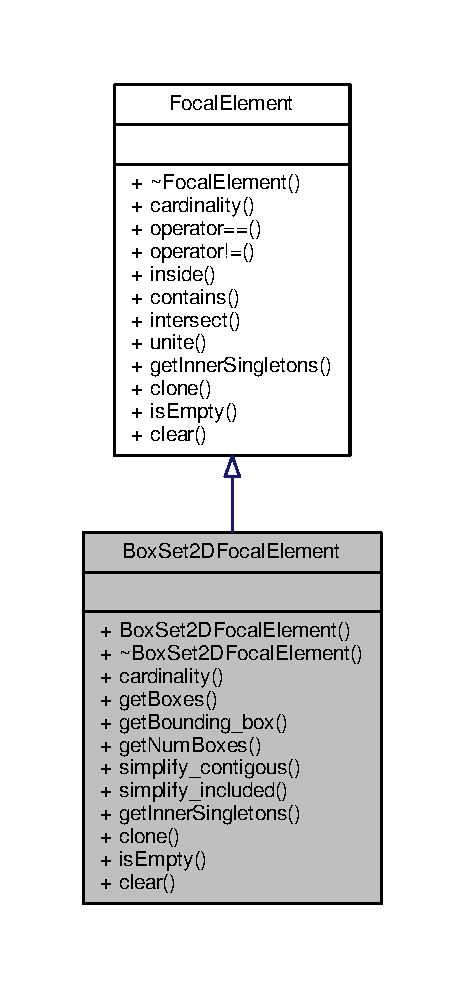
\includegraphics[width=223pt]{classBoxSet2DFocalElement__inherit__graph}
\end{center}
\end{figure}


Collaboration diagram for Box\+Set2\+D\+Focal\+Element\+:\nopagebreak
\begin{figure}[H]
\begin{center}
\leavevmode
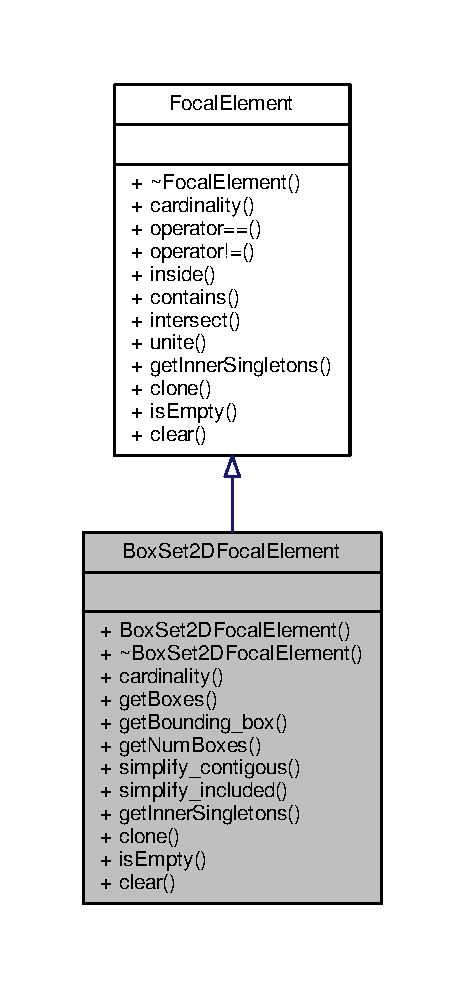
\includegraphics[width=223pt]{classBoxSet2DFocalElement__coll__graph}
\end{center}
\end{figure}
\subsection*{Public Member Functions}
\begin{DoxyCompactItemize}
\item 
\hyperlink{classBoxSet2DFocalElement_a8215ede5350376e541893ce73d8e5a05}{Box\+Set2\+D\+Focal\+Element} (const std\+::vector$<$ \hyperlink{classGeometry_1_1Rectangle}{Geometry\+::\+Rectangle} $>$ \&boxes)
\begin{DoxyCompactList}\small\item\em Constructor. \end{DoxyCompactList}\item 
\hyperlink{classBoxSet2DFocalElement_aca7b4a88ffdd6b3d1e8b688c4f2e13ba}{$\sim$\+Box\+Set2\+D\+Focal\+Element} () override=default
\item 
double \hyperlink{classBoxSet2DFocalElement_a65dd4942ec406f9048432654f81df964}{cardinality} () const override
\begin{DoxyCompactList}\small\item\em Evaluate the cardinality of the focal element. \end{DoxyCompactList}\item 
const std\+::vector$<$ \hyperlink{classGeometry_1_1Rectangle}{Geometry\+::\+Rectangle} $>$ \& \hyperlink{classBoxSet2DFocalElement_a21707f3b23e1d1b72db05ccfae023634}{get\+Boxes} () const 
\begin{DoxyCompactList}\small\item\em Get the boxes. \end{DoxyCompactList}\item 
const \hyperlink{classGeometry_1_1Rectangle}{Geometry\+::\+Rectangle} \& \hyperlink{classBoxSet2DFocalElement_a431361485288f14e2770aab9d12a1320}{get\+Bounding\+\_\+box} () const 
\begin{DoxyCompactList}\small\item\em Get the bounding box. \end{DoxyCompactList}\item 
size\+\_\+t \hyperlink{classBoxSet2DFocalElement_aea0ef3a8e8f6e64e1305400771590749}{get\+Num\+Boxes} ()
\begin{DoxyCompactList}\small\item\em Get the number of boxes. \end{DoxyCompactList}\item 
void \hyperlink{classBoxSet2DFocalElement_a48eaa6fae893da98034ea1359bb6a6da}{simplify\+\_\+contigous} ()
\begin{DoxyCompactList}\small\item\em Simplify representation fusing contigous rectangles. \end{DoxyCompactList}\item 
void \hyperlink{classBoxSet2DFocalElement_a8e80a0fb79597dfa97e7d2d4ef49623d}{simplify\+\_\+included} ()
\begin{DoxyCompactList}\small\item\em Simplify representation with inclusion test. \end{DoxyCompactList}\item 
std\+::vector$<$ std\+::unique\+\_\+ptr$<$ \hyperlink{classFocalElement}{Focal\+Element} $>$ $>$ \hyperlink{classBoxSet2DFocalElement_afdd0db628fc45a5865c72d9f1fb3fcce}{get\+Inner\+Singletons} (\hyperlink{CMakeCache_8txt_a79a3d8790b2588b09777910863574e09}{int} step\+\_\+size=1) const override
\begin{DoxyCompactList}\small\item\em Extract the singleton Focal\+Elements included in the current one. \end{DoxyCompactList}\item 
std\+::unique\+\_\+ptr$<$ \hyperlink{classFocalElement}{Focal\+Element} $>$ \hyperlink{classBoxSet2DFocalElement_a0e325a4cad33db05c423f46eb1f346c9}{clone} () const override
\begin{DoxyCompactList}\small\item\em Clone method. \end{DoxyCompactList}\item 
bool \hyperlink{classBoxSet2DFocalElement_a7512305b698f37aa77f3acacd0626f77}{is\+Empty} () const override
\begin{DoxyCompactList}\small\item\em Check whether the current \hyperlink{classFocalElement}{Focal\+Element} is the empty set. \end{DoxyCompactList}\item 
void \hyperlink{classBoxSet2DFocalElement_a9b09d64e1511def1a20898c7e3ac7390}{clear} () override
\begin{DoxyCompactList}\small\item\em Clear the \hyperlink{classFocalElement}{Focal\+Element}, resulting into the empty set. \end{DoxyCompactList}\end{DoxyCompactItemize}


\subsection{Detailed Description}
2D \hyperlink{classFocalElement}{Focal\+Element} expressed as a set of rectangles. 

\subsection{Constructor \& Destructor Documentation}
\index{Box\+Set2\+D\+Focal\+Element@{Box\+Set2\+D\+Focal\+Element}!Box\+Set2\+D\+Focal\+Element@{Box\+Set2\+D\+Focal\+Element}}
\index{Box\+Set2\+D\+Focal\+Element@{Box\+Set2\+D\+Focal\+Element}!Box\+Set2\+D\+Focal\+Element@{Box\+Set2\+D\+Focal\+Element}}
\subsubsection[{\texorpdfstring{Box\+Set2\+D\+Focal\+Element(const std\+::vector$<$ Geometry\+::\+Rectangle $>$ \&boxes)}{BoxSet2DFocalElement(const std::vector< Geometry::Rectangle > &boxes)}}]{\setlength{\rightskip}{0pt plus 5cm}Box\+Set2\+D\+Focal\+Element\+::\+Box\+Set2\+D\+Focal\+Element (
\begin{DoxyParamCaption}
\item[{const std\+::vector$<$ {\bf Geometry\+::\+Rectangle} $>$ \&}]{boxes}
\end{DoxyParamCaption}
)\hspace{0.3cm}{\ttfamily [explicit]}}\hypertarget{classBoxSet2DFocalElement_a8215ede5350376e541893ce73d8e5a05}{}\label{classBoxSet2DFocalElement_a8215ede5350376e541893ce73d8e5a05}


Constructor. 


\begin{DoxyParams}{Parameters}
{\em boxes} & Array of boxes. \\
\hline
\end{DoxyParams}
\index{Box\+Set2\+D\+Focal\+Element@{Box\+Set2\+D\+Focal\+Element}!````~Box\+Set2\+D\+Focal\+Element@{$\sim$\+Box\+Set2\+D\+Focal\+Element}}
\index{````~Box\+Set2\+D\+Focal\+Element@{$\sim$\+Box\+Set2\+D\+Focal\+Element}!Box\+Set2\+D\+Focal\+Element@{Box\+Set2\+D\+Focal\+Element}}
\subsubsection[{\texorpdfstring{$\sim$\+Box\+Set2\+D\+Focal\+Element() override=default}{~BoxSet2DFocalElement() override=default}}]{\setlength{\rightskip}{0pt plus 5cm}Box\+Set2\+D\+Focal\+Element\+::$\sim$\+Box\+Set2\+D\+Focal\+Element (
\begin{DoxyParamCaption}
{}
\end{DoxyParamCaption}
)\hspace{0.3cm}{\ttfamily [override]}, {\ttfamily [default]}}\hypertarget{classBoxSet2DFocalElement_aca7b4a88ffdd6b3d1e8b688c4f2e13ba}{}\label{classBoxSet2DFocalElement_aca7b4a88ffdd6b3d1e8b688c4f2e13ba}


\subsection{Member Function Documentation}
\index{Box\+Set2\+D\+Focal\+Element@{Box\+Set2\+D\+Focal\+Element}!cardinality@{cardinality}}
\index{cardinality@{cardinality}!Box\+Set2\+D\+Focal\+Element@{Box\+Set2\+D\+Focal\+Element}}
\subsubsection[{\texorpdfstring{cardinality() const override}{cardinality() const override}}]{\setlength{\rightskip}{0pt plus 5cm}double Box\+Set2\+D\+Focal\+Element\+::cardinality (
\begin{DoxyParamCaption}
{}
\end{DoxyParamCaption}
) const\hspace{0.3cm}{\ttfamily [override]}, {\ttfamily [virtual]}}\hypertarget{classBoxSet2DFocalElement_a65dd4942ec406f9048432654f81df964}{}\label{classBoxSet2DFocalElement_a65dd4942ec406f9048432654f81df964}


Evaluate the cardinality of the focal element. 

\begin{DoxyReturn}{Returns}
Cardinality of the set. 
\end{DoxyReturn}


Implements \hyperlink{classFocalElement_a4ab1bbd0875e6e7ce2d7fe152e6a1639}{Focal\+Element}.

\index{Box\+Set2\+D\+Focal\+Element@{Box\+Set2\+D\+Focal\+Element}!clear@{clear}}
\index{clear@{clear}!Box\+Set2\+D\+Focal\+Element@{Box\+Set2\+D\+Focal\+Element}}
\subsubsection[{\texorpdfstring{clear() override}{clear() override}}]{\setlength{\rightskip}{0pt plus 5cm}void Box\+Set2\+D\+Focal\+Element\+::clear (
\begin{DoxyParamCaption}
{}
\end{DoxyParamCaption}
)\hspace{0.3cm}{\ttfamily [override]}, {\ttfamily [virtual]}}\hypertarget{classBoxSet2DFocalElement_a9b09d64e1511def1a20898c7e3ac7390}{}\label{classBoxSet2DFocalElement_a9b09d64e1511def1a20898c7e3ac7390}


Clear the \hyperlink{classFocalElement}{Focal\+Element}, resulting into the empty set. 



Implements \hyperlink{classFocalElement_a635cb4afffa2dc69cf9fc9ff94a6d90f}{Focal\+Element}.

\index{Box\+Set2\+D\+Focal\+Element@{Box\+Set2\+D\+Focal\+Element}!clone@{clone}}
\index{clone@{clone}!Box\+Set2\+D\+Focal\+Element@{Box\+Set2\+D\+Focal\+Element}}
\subsubsection[{\texorpdfstring{clone() const override}{clone() const override}}]{\setlength{\rightskip}{0pt plus 5cm}std\+::unique\+\_\+ptr$<$ {\bf Focal\+Element} $>$ Box\+Set2\+D\+Focal\+Element\+::clone (
\begin{DoxyParamCaption}
{}
\end{DoxyParamCaption}
) const\hspace{0.3cm}{\ttfamily [override]}, {\ttfamily [virtual]}}\hypertarget{classBoxSet2DFocalElement_a0e325a4cad33db05c423f46eb1f346c9}{}\label{classBoxSet2DFocalElement_a0e325a4cad33db05c423f46eb1f346c9}


Clone method. 

\begin{DoxyReturn}{Returns}
A copy of the current \hyperlink{classFocalElement}{Focal\+Element}. 
\end{DoxyReturn}


Implements \hyperlink{classFocalElement_a21697fbbbcb144c18fa7b4ecae5e6145}{Focal\+Element}.

\index{Box\+Set2\+D\+Focal\+Element@{Box\+Set2\+D\+Focal\+Element}!get\+Bounding\+\_\+box@{get\+Bounding\+\_\+box}}
\index{get\+Bounding\+\_\+box@{get\+Bounding\+\_\+box}!Box\+Set2\+D\+Focal\+Element@{Box\+Set2\+D\+Focal\+Element}}
\subsubsection[{\texorpdfstring{get\+Bounding\+\_\+box() const }{getBounding_box() const }}]{\setlength{\rightskip}{0pt plus 5cm}const {\bf Geometry\+::\+Rectangle} \& Box\+Set2\+D\+Focal\+Element\+::get\+Bounding\+\_\+box (
\begin{DoxyParamCaption}
{}
\end{DoxyParamCaption}
) const}\hypertarget{classBoxSet2DFocalElement_a431361485288f14e2770aab9d12a1320}{}\label{classBoxSet2DFocalElement_a431361485288f14e2770aab9d12a1320}


Get the bounding box. 

The bounding box is the smallest rectangle containing all the boxes. \begin{DoxyReturn}{Returns}
The bounding box. 
\end{DoxyReturn}
\index{Box\+Set2\+D\+Focal\+Element@{Box\+Set2\+D\+Focal\+Element}!get\+Boxes@{get\+Boxes}}
\index{get\+Boxes@{get\+Boxes}!Box\+Set2\+D\+Focal\+Element@{Box\+Set2\+D\+Focal\+Element}}
\subsubsection[{\texorpdfstring{get\+Boxes() const }{getBoxes() const }}]{\setlength{\rightskip}{0pt plus 5cm}const std\+::vector$<$ {\bf Geometry\+::\+Rectangle} $>$ \& Box\+Set2\+D\+Focal\+Element\+::get\+Boxes (
\begin{DoxyParamCaption}
{}
\end{DoxyParamCaption}
) const}\hypertarget{classBoxSet2DFocalElement_a21707f3b23e1d1b72db05ccfae023634}{}\label{classBoxSet2DFocalElement_a21707f3b23e1d1b72db05ccfae023634}


Get the boxes. 

\begin{DoxyReturn}{Returns}
Array of rectangles. 
\end{DoxyReturn}
\index{Box\+Set2\+D\+Focal\+Element@{Box\+Set2\+D\+Focal\+Element}!get\+Inner\+Singletons@{get\+Inner\+Singletons}}
\index{get\+Inner\+Singletons@{get\+Inner\+Singletons}!Box\+Set2\+D\+Focal\+Element@{Box\+Set2\+D\+Focal\+Element}}
\subsubsection[{\texorpdfstring{get\+Inner\+Singletons(int step\+\_\+size=1) const override}{getInnerSingletons(int step_size=1) const override}}]{\setlength{\rightskip}{0pt plus 5cm}std\+::vector$<$ std\+::unique\+\_\+ptr$<$ {\bf Focal\+Element} $>$ $>$ Box\+Set2\+D\+Focal\+Element\+::get\+Inner\+Singletons (
\begin{DoxyParamCaption}
\item[{{\bf int}}]{step\+\_\+size = {\ttfamily 1}}
\end{DoxyParamCaption}
) const\hspace{0.3cm}{\ttfamily [override]}, {\ttfamily [virtual]}}\hypertarget{classBoxSet2DFocalElement_afdd0db628fc45a5865c72d9f1fb3fcce}{}\label{classBoxSet2DFocalElement_afdd0db628fc45a5865c72d9f1fb3fcce}


Extract the singleton Focal\+Elements included in the current one. 


\begin{DoxyParams}{Parameters}
{\em step\+\_\+size} & The sampling resulution. Step\+\_\+size=1 means that all the singletons are retrieved. Step\+\_\+size $>$ 1 means that singletons are sampled for performance reason. \\
\hline
\end{DoxyParams}
\begin{DoxyReturn}{Returns}
Array of singleton Focal\+Elements. 
\end{DoxyReturn}


Implements \hyperlink{classFocalElement_ac615e960ea64a4bdc0f442135f6069e2}{Focal\+Element}.

\index{Box\+Set2\+D\+Focal\+Element@{Box\+Set2\+D\+Focal\+Element}!get\+Num\+Boxes@{get\+Num\+Boxes}}
\index{get\+Num\+Boxes@{get\+Num\+Boxes}!Box\+Set2\+D\+Focal\+Element@{Box\+Set2\+D\+Focal\+Element}}
\subsubsection[{\texorpdfstring{get\+Num\+Boxes()}{getNumBoxes()}}]{\setlength{\rightskip}{0pt plus 5cm}size\+\_\+t Box\+Set2\+D\+Focal\+Element\+::get\+Num\+Boxes (
\begin{DoxyParamCaption}
{}
\end{DoxyParamCaption}
)}\hypertarget{classBoxSet2DFocalElement_aea0ef3a8e8f6e64e1305400771590749}{}\label{classBoxSet2DFocalElement_aea0ef3a8e8f6e64e1305400771590749}


Get the number of boxes. 

\begin{DoxyReturn}{Returns}
Size of the boxes array. 
\end{DoxyReturn}
\index{Box\+Set2\+D\+Focal\+Element@{Box\+Set2\+D\+Focal\+Element}!is\+Empty@{is\+Empty}}
\index{is\+Empty@{is\+Empty}!Box\+Set2\+D\+Focal\+Element@{Box\+Set2\+D\+Focal\+Element}}
\subsubsection[{\texorpdfstring{is\+Empty() const override}{isEmpty() const override}}]{\setlength{\rightskip}{0pt plus 5cm}bool Box\+Set2\+D\+Focal\+Element\+::is\+Empty (
\begin{DoxyParamCaption}
{}
\end{DoxyParamCaption}
) const\hspace{0.3cm}{\ttfamily [override]}, {\ttfamily [virtual]}}\hypertarget{classBoxSet2DFocalElement_a7512305b698f37aa77f3acacd0626f77}{}\label{classBoxSet2DFocalElement_a7512305b698f37aa77f3acacd0626f77}


Check whether the current \hyperlink{classFocalElement}{Focal\+Element} is the empty set. 

\begin{DoxyReturn}{Returns}
True if the object is the empty set. 
\end{DoxyReturn}


Implements \hyperlink{classFocalElement_aed131a65fdfc885019f9bf8f1d454508}{Focal\+Element}.

\index{Box\+Set2\+D\+Focal\+Element@{Box\+Set2\+D\+Focal\+Element}!simplify\+\_\+contigous@{simplify\+\_\+contigous}}
\index{simplify\+\_\+contigous@{simplify\+\_\+contigous}!Box\+Set2\+D\+Focal\+Element@{Box\+Set2\+D\+Focal\+Element}}
\subsubsection[{\texorpdfstring{simplify\+\_\+contigous()}{simplify_contigous()}}]{\setlength{\rightskip}{0pt plus 5cm}void Box\+Set2\+D\+Focal\+Element\+::simplify\+\_\+contigous (
\begin{DoxyParamCaption}
{}
\end{DoxyParamCaption}
)}\hypertarget{classBoxSet2DFocalElement_a48eaa6fae893da98034ea1359bb6a6da}{}\label{classBoxSet2DFocalElement_a48eaa6fae893da98034ea1359bb6a6da}


Simplify representation fusing contigous rectangles. 

\index{Box\+Set2\+D\+Focal\+Element@{Box\+Set2\+D\+Focal\+Element}!simplify\+\_\+included@{simplify\+\_\+included}}
\index{simplify\+\_\+included@{simplify\+\_\+included}!Box\+Set2\+D\+Focal\+Element@{Box\+Set2\+D\+Focal\+Element}}
\subsubsection[{\texorpdfstring{simplify\+\_\+included()}{simplify_included()}}]{\setlength{\rightskip}{0pt plus 5cm}void Box\+Set2\+D\+Focal\+Element\+::simplify\+\_\+included (
\begin{DoxyParamCaption}
{}
\end{DoxyParamCaption}
)}\hypertarget{classBoxSet2DFocalElement_a8e80a0fb79597dfa97e7d2d4ef49623d}{}\label{classBoxSet2DFocalElement_a8e80a0fb79597dfa97e7d2d4ef49623d}


Simplify representation with inclusion test. 



The documentation for this class was generated from the following files\+:\begin{DoxyCompactItemize}
\item 
focal\+\_\+elements/\hyperlink{BoxSet2DFocalElement_8h}{Box\+Set2\+D\+Focal\+Element.\+h}\item 
focal\+\_\+elements/\hyperlink{BoxSet2DFocalElement_8cpp}{Box\+Set2\+D\+Focal\+Element.\+cpp}\end{DoxyCompactItemize}

\hypertarget{classClipper2DFocalElement}{}\section{Clipper2\+D\+Focal\+Element Class Reference}
\label{classClipper2DFocalElement}\index{Clipper2\+D\+Focal\+Element@{Clipper2\+D\+Focal\+Element}}


2D \hyperlink{classFocalElement}{Focal\+Element} using the \href{http://www.angusj.com/delphi/clipper.php}{\tt Clipper library}  




{\ttfamily \#include $<$Clipper2\+D\+Focal\+Element.\+h$>$}



Inheritance diagram for Clipper2\+D\+Focal\+Element\+:\nopagebreak
\begin{figure}[H]
\begin{center}
\leavevmode
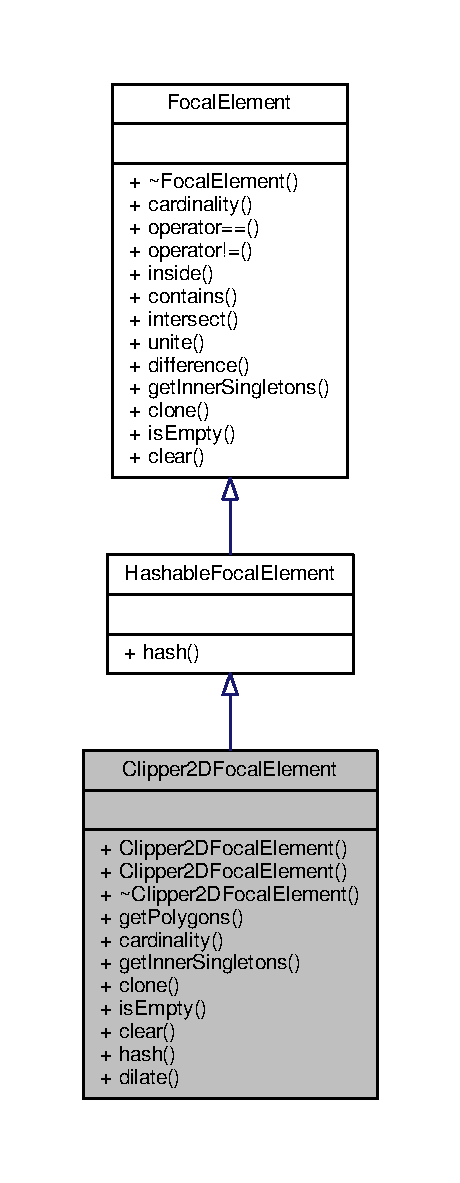
\includegraphics[height=550pt]{classClipper2DFocalElement__inherit__graph}
\end{center}
\end{figure}


Collaboration diagram for Clipper2\+D\+Focal\+Element\+:\nopagebreak
\begin{figure}[H]
\begin{center}
\leavevmode
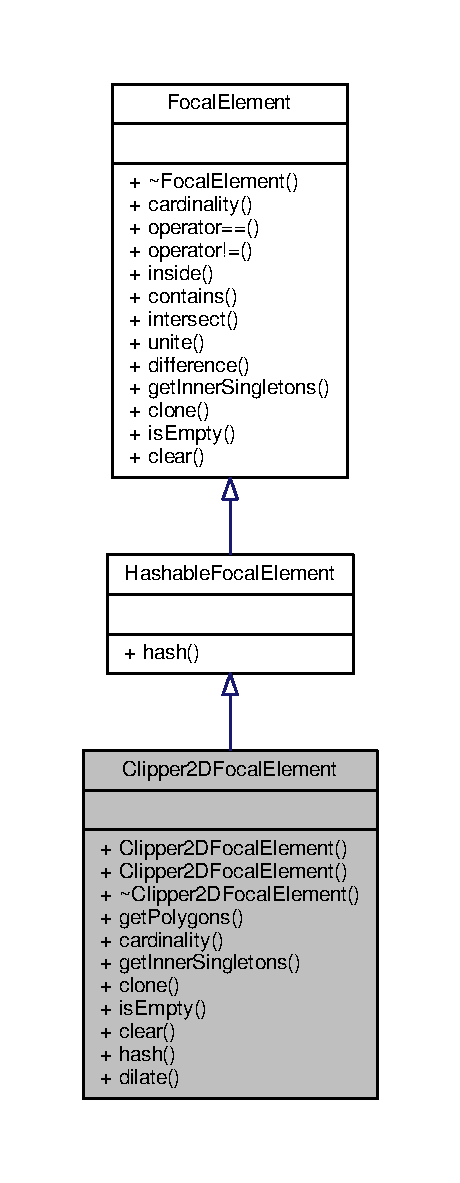
\includegraphics[height=550pt]{classClipper2DFocalElement__coll__graph}
\end{center}
\end{figure}
\subsection*{Public Member Functions}
\begin{DoxyCompactItemize}
\item 
\hyperlink{classClipper2DFocalElement_ae8687e5aa208657a22429ac63182f183}{Clipper2\+D\+Focal\+Element} (std\+::vector$<$ \hyperlink{classGeometry_1_1ClipperPolygon}{Geometry\+::\+Clipper\+Polygon} $>$ polygons)
\begin{DoxyCompactList}\small\item\em Constructor. \end{DoxyCompactList}\item 
\hyperlink{classClipper2DFocalElement_a908a30532e268e886458fbd3793874b3}{Clipper2\+D\+Focal\+Element} (\hyperlink{classGeometry_1_1ClipperPolygon}{Geometry\+::\+Clipper\+Polygon} polygon)
\begin{DoxyCompactList}\small\item\em Constructor. \end{DoxyCompactList}\item 
\hyperlink{classClipper2DFocalElement_a69afddff55e6195330e864f33e78559a}{$\sim$\+Clipper2\+D\+Focal\+Element} () override=default
\item 
const std\+::vector$<$ \hyperlink{classGeometry_1_1ClipperPolygon}{Geometry\+::\+Clipper\+Polygon} $>$ \& \hyperlink{classClipper2DFocalElement_a933998b031a0063252d7aa63cd0cd145}{get\+Polygons} () const 
\begin{DoxyCompactList}\small\item\em Get the array of polygons. \end{DoxyCompactList}\item 
double \hyperlink{classClipper2DFocalElement_a8eabcd9808b5b6bb7ec2f26eb89b5cd9}{cardinality} () const override
\begin{DoxyCompactList}\small\item\em Evaluate the cardinality of the focal element. \end{DoxyCompactList}\item 
std\+::vector$<$ std\+::unique\+\_\+ptr$<$ \hyperlink{classFocalElement}{Focal\+Element} $>$ $>$ \hyperlink{classClipper2DFocalElement_a2455cb3cc5940ecee3e012bcdcc25f44}{get\+Inner\+Singletons} (\hyperlink{CMakeCache_8txt_a79a3d8790b2588b09777910863574e09}{int} step\+\_\+size=1) const override
\begin{DoxyCompactList}\small\item\em Extract the singleton Focal\+Elements included in the current one. \end{DoxyCompactList}\item 
std\+::unique\+\_\+ptr$<$ \hyperlink{classFocalElement}{Focal\+Element} $>$ \hyperlink{classClipper2DFocalElement_a43aa82869ed3bf22682907ec9c475930}{clone} () const override
\begin{DoxyCompactList}\small\item\em Clone method. \end{DoxyCompactList}\item 
bool \hyperlink{classClipper2DFocalElement_ae79aa59bb6a1109d729a32240631d573}{is\+Empty} () const override
\begin{DoxyCompactList}\small\item\em Check whether the current \hyperlink{classFocalElement}{Focal\+Element} is the empty set. \end{DoxyCompactList}\item 
void \hyperlink{classClipper2DFocalElement_aa1110dabb3e01c681826374d1a485670}{clear} () override
\begin{DoxyCompactList}\small\item\em Clear the \hyperlink{classFocalElement}{Focal\+Element}, resulting into the empty set. \end{DoxyCompactList}\item 
size\+\_\+t \hyperlink{classClipper2DFocalElement_a005167e2e6d599b1f9f1bb77352add90}{hash} () const override
\begin{DoxyCompactList}\small\item\em Compute the hash function. \end{DoxyCompactList}\item 
std\+::unique\+\_\+ptr$<$ \hyperlink{classFocalElement}{Focal\+Element} $>$ \hyperlink{classClipper2DFocalElement_a23fd6a49f14917ec9a539562c129d945}{dilate} (long delta)
\begin{DoxyCompactList}\small\item\em Perform polygon offsetting of the current focal element. \end{DoxyCompactList}\end{DoxyCompactItemize}


\subsection{Detailed Description}
2D \hyperlink{classFocalElement}{Focal\+Element} using the \href{http://www.angusj.com/delphi/clipper.php}{\tt Clipper library} 

\subsection{Constructor \& Destructor Documentation}
\index{Clipper2\+D\+Focal\+Element@{Clipper2\+D\+Focal\+Element}!Clipper2\+D\+Focal\+Element@{Clipper2\+D\+Focal\+Element}}
\index{Clipper2\+D\+Focal\+Element@{Clipper2\+D\+Focal\+Element}!Clipper2\+D\+Focal\+Element@{Clipper2\+D\+Focal\+Element}}
\subsubsection[{\texorpdfstring{Clipper2\+D\+Focal\+Element(std\+::vector$<$ Geometry\+::\+Clipper\+Polygon $>$ polygons)}{Clipper2DFocalElement(std::vector< Geometry::ClipperPolygon > polygons)}}]{\setlength{\rightskip}{0pt plus 5cm}Clipper2\+D\+Focal\+Element\+::\+Clipper2\+D\+Focal\+Element (
\begin{DoxyParamCaption}
\item[{std\+::vector$<$ {\bf Geometry\+::\+Clipper\+Polygon} $>$}]{polygons}
\end{DoxyParamCaption}
)\hspace{0.3cm}{\ttfamily [explicit]}}\hypertarget{classClipper2DFocalElement_ae8687e5aa208657a22429ac63182f183}{}\label{classClipper2DFocalElement_ae8687e5aa208657a22429ac63182f183}


Constructor. 


\begin{DoxyParams}{Parameters}
{\em polygons} & Array of polygons. \\
\hline
\end{DoxyParams}
\index{Clipper2\+D\+Focal\+Element@{Clipper2\+D\+Focal\+Element}!Clipper2\+D\+Focal\+Element@{Clipper2\+D\+Focal\+Element}}
\index{Clipper2\+D\+Focal\+Element@{Clipper2\+D\+Focal\+Element}!Clipper2\+D\+Focal\+Element@{Clipper2\+D\+Focal\+Element}}
\subsubsection[{\texorpdfstring{Clipper2\+D\+Focal\+Element(\+Geometry\+::\+Clipper\+Polygon polygon)}{Clipper2DFocalElement(Geometry::ClipperPolygon polygon)}}]{\setlength{\rightskip}{0pt plus 5cm}Clipper2\+D\+Focal\+Element\+::\+Clipper2\+D\+Focal\+Element (
\begin{DoxyParamCaption}
\item[{{\bf Geometry\+::\+Clipper\+Polygon}}]{polygon}
\end{DoxyParamCaption}
)\hspace{0.3cm}{\ttfamily [explicit]}}\hypertarget{classClipper2DFocalElement_a908a30532e268e886458fbd3793874b3}{}\label{classClipper2DFocalElement_a908a30532e268e886458fbd3793874b3}


Constructor. 


\begin{DoxyParams}{Parameters}
{\em polygons} & Single polygon. \\
\hline
\end{DoxyParams}
\index{Clipper2\+D\+Focal\+Element@{Clipper2\+D\+Focal\+Element}!````~Clipper2\+D\+Focal\+Element@{$\sim$\+Clipper2\+D\+Focal\+Element}}
\index{````~Clipper2\+D\+Focal\+Element@{$\sim$\+Clipper2\+D\+Focal\+Element}!Clipper2\+D\+Focal\+Element@{Clipper2\+D\+Focal\+Element}}
\subsubsection[{\texorpdfstring{$\sim$\+Clipper2\+D\+Focal\+Element() override=default}{~Clipper2DFocalElement() override=default}}]{\setlength{\rightskip}{0pt plus 5cm}Clipper2\+D\+Focal\+Element\+::$\sim$\+Clipper2\+D\+Focal\+Element (
\begin{DoxyParamCaption}
{}
\end{DoxyParamCaption}
)\hspace{0.3cm}{\ttfamily [override]}, {\ttfamily [default]}}\hypertarget{classClipper2DFocalElement_a69afddff55e6195330e864f33e78559a}{}\label{classClipper2DFocalElement_a69afddff55e6195330e864f33e78559a}


\subsection{Member Function Documentation}
\index{Clipper2\+D\+Focal\+Element@{Clipper2\+D\+Focal\+Element}!cardinality@{cardinality}}
\index{cardinality@{cardinality}!Clipper2\+D\+Focal\+Element@{Clipper2\+D\+Focal\+Element}}
\subsubsection[{\texorpdfstring{cardinality() const override}{cardinality() const override}}]{\setlength{\rightskip}{0pt plus 5cm}double Clipper2\+D\+Focal\+Element\+::cardinality (
\begin{DoxyParamCaption}
{}
\end{DoxyParamCaption}
) const\hspace{0.3cm}{\ttfamily [override]}, {\ttfamily [virtual]}}\hypertarget{classClipper2DFocalElement_a8eabcd9808b5b6bb7ec2f26eb89b5cd9}{}\label{classClipper2DFocalElement_a8eabcd9808b5b6bb7ec2f26eb89b5cd9}


Evaluate the cardinality of the focal element. 

\begin{DoxyReturn}{Returns}
Cardinality of the set. 
\end{DoxyReturn}


Implements \hyperlink{classFocalElement_a4ab1bbd0875e6e7ce2d7fe152e6a1639}{Focal\+Element}.

\index{Clipper2\+D\+Focal\+Element@{Clipper2\+D\+Focal\+Element}!clear@{clear}}
\index{clear@{clear}!Clipper2\+D\+Focal\+Element@{Clipper2\+D\+Focal\+Element}}
\subsubsection[{\texorpdfstring{clear() override}{clear() override}}]{\setlength{\rightskip}{0pt plus 5cm}void Clipper2\+D\+Focal\+Element\+::clear (
\begin{DoxyParamCaption}
{}
\end{DoxyParamCaption}
)\hspace{0.3cm}{\ttfamily [override]}, {\ttfamily [virtual]}}\hypertarget{classClipper2DFocalElement_aa1110dabb3e01c681826374d1a485670}{}\label{classClipper2DFocalElement_aa1110dabb3e01c681826374d1a485670}


Clear the \hyperlink{classFocalElement}{Focal\+Element}, resulting into the empty set. 



Implements \hyperlink{classFocalElement_a635cb4afffa2dc69cf9fc9ff94a6d90f}{Focal\+Element}.

\index{Clipper2\+D\+Focal\+Element@{Clipper2\+D\+Focal\+Element}!clone@{clone}}
\index{clone@{clone}!Clipper2\+D\+Focal\+Element@{Clipper2\+D\+Focal\+Element}}
\subsubsection[{\texorpdfstring{clone() const override}{clone() const override}}]{\setlength{\rightskip}{0pt plus 5cm}std\+::unique\+\_\+ptr$<$ {\bf Focal\+Element} $>$ Clipper2\+D\+Focal\+Element\+::clone (
\begin{DoxyParamCaption}
{}
\end{DoxyParamCaption}
) const\hspace{0.3cm}{\ttfamily [override]}, {\ttfamily [virtual]}}\hypertarget{classClipper2DFocalElement_a43aa82869ed3bf22682907ec9c475930}{}\label{classClipper2DFocalElement_a43aa82869ed3bf22682907ec9c475930}


Clone method. 

\begin{DoxyReturn}{Returns}
A copy of the current \hyperlink{classFocalElement}{Focal\+Element}. 
\end{DoxyReturn}


Implements \hyperlink{classFocalElement_a21697fbbbcb144c18fa7b4ecae5e6145}{Focal\+Element}.

\index{Clipper2\+D\+Focal\+Element@{Clipper2\+D\+Focal\+Element}!dilate@{dilate}}
\index{dilate@{dilate}!Clipper2\+D\+Focal\+Element@{Clipper2\+D\+Focal\+Element}}
\subsubsection[{\texorpdfstring{dilate(long delta)}{dilate(long delta)}}]{\setlength{\rightskip}{0pt plus 5cm}std\+::unique\+\_\+ptr$<$ {\bf Focal\+Element} $>$ Clipper2\+D\+Focal\+Element\+::dilate (
\begin{DoxyParamCaption}
\item[{long}]{delta}
\end{DoxyParamCaption}
)}\hypertarget{classClipper2DFocalElement_a23fd6a49f14917ec9a539562c129d945}{}\label{classClipper2DFocalElement_a23fd6a49f14917ec9a539562c129d945}


Perform polygon offsetting of the current focal element. 


\begin{DoxyParams}{Parameters}
{\em delta} & Offsetting radius. \\
\hline
\end{DoxyParams}
\begin{DoxyReturn}{Returns}
The dilated focal element. 
\end{DoxyReturn}
\index{Clipper2\+D\+Focal\+Element@{Clipper2\+D\+Focal\+Element}!get\+Inner\+Singletons@{get\+Inner\+Singletons}}
\index{get\+Inner\+Singletons@{get\+Inner\+Singletons}!Clipper2\+D\+Focal\+Element@{Clipper2\+D\+Focal\+Element}}
\subsubsection[{\texorpdfstring{get\+Inner\+Singletons(int step\+\_\+size=1) const override}{getInnerSingletons(int step_size=1) const override}}]{\setlength{\rightskip}{0pt plus 5cm}std\+::vector$<$ std\+::unique\+\_\+ptr$<$ {\bf Focal\+Element} $>$ $>$ Clipper2\+D\+Focal\+Element\+::get\+Inner\+Singletons (
\begin{DoxyParamCaption}
\item[{{\bf int}}]{step\+\_\+size = {\ttfamily 1}}
\end{DoxyParamCaption}
) const\hspace{0.3cm}{\ttfamily [override]}, {\ttfamily [virtual]}}\hypertarget{classClipper2DFocalElement_a2455cb3cc5940ecee3e012bcdcc25f44}{}\label{classClipper2DFocalElement_a2455cb3cc5940ecee3e012bcdcc25f44}


Extract the singleton Focal\+Elements included in the current one. 


\begin{DoxyParams}{Parameters}
{\em step\+\_\+size} & The sampling resulution. Step\+\_\+size=1 means that all the singletons are retrieved. Step\+\_\+size $>$ 1 means that singletons are sampled for performance reason. \\
\hline
\end{DoxyParams}
\begin{DoxyReturn}{Returns}
Array of singleton Focal\+Elements. 
\end{DoxyReturn}


Implements \hyperlink{classFocalElement_ac615e960ea64a4bdc0f442135f6069e2}{Focal\+Element}.

\index{Clipper2\+D\+Focal\+Element@{Clipper2\+D\+Focal\+Element}!get\+Polygons@{get\+Polygons}}
\index{get\+Polygons@{get\+Polygons}!Clipper2\+D\+Focal\+Element@{Clipper2\+D\+Focal\+Element}}
\subsubsection[{\texorpdfstring{get\+Polygons() const }{getPolygons() const }}]{\setlength{\rightskip}{0pt plus 5cm}const std\+::vector$<$ {\bf Geometry\+::\+Clipper\+Polygon} $>$ \& Clipper2\+D\+Focal\+Element\+::get\+Polygons (
\begin{DoxyParamCaption}
{}
\end{DoxyParamCaption}
) const}\hypertarget{classClipper2DFocalElement_a933998b031a0063252d7aa63cd0cd145}{}\label{classClipper2DFocalElement_a933998b031a0063252d7aa63cd0cd145}


Get the array of polygons. 

\begin{DoxyReturn}{Returns}
Array of Clipper\+Polygon objects. 
\end{DoxyReturn}
\index{Clipper2\+D\+Focal\+Element@{Clipper2\+D\+Focal\+Element}!hash@{hash}}
\index{hash@{hash}!Clipper2\+D\+Focal\+Element@{Clipper2\+D\+Focal\+Element}}
\subsubsection[{\texorpdfstring{hash() const override}{hash() const override}}]{\setlength{\rightskip}{0pt plus 5cm}size\+\_\+t Clipper2\+D\+Focal\+Element\+::hash (
\begin{DoxyParamCaption}
{}
\end{DoxyParamCaption}
) const\hspace{0.3cm}{\ttfamily [override]}, {\ttfamily [virtual]}}\hypertarget{classClipper2DFocalElement_a005167e2e6d599b1f9f1bb77352add90}{}\label{classClipper2DFocalElement_a005167e2e6d599b1f9f1bb77352add90}


Compute the hash function. 

\begin{DoxyReturn}{Returns}
The value of the hash. 
\end{DoxyReturn}


Implements \hyperlink{classHashableFocalElement_a8b7bfbf1e107fa5a6cfc5033db196c63}{Hashable\+Focal\+Element}.

\index{Clipper2\+D\+Focal\+Element@{Clipper2\+D\+Focal\+Element}!is\+Empty@{is\+Empty}}
\index{is\+Empty@{is\+Empty}!Clipper2\+D\+Focal\+Element@{Clipper2\+D\+Focal\+Element}}
\subsubsection[{\texorpdfstring{is\+Empty() const override}{isEmpty() const override}}]{\setlength{\rightskip}{0pt plus 5cm}bool Clipper2\+D\+Focal\+Element\+::is\+Empty (
\begin{DoxyParamCaption}
{}
\end{DoxyParamCaption}
) const\hspace{0.3cm}{\ttfamily [override]}, {\ttfamily [virtual]}}\hypertarget{classClipper2DFocalElement_ae79aa59bb6a1109d729a32240631d573}{}\label{classClipper2DFocalElement_ae79aa59bb6a1109d729a32240631d573}


Check whether the current \hyperlink{classFocalElement}{Focal\+Element} is the empty set. 

\begin{DoxyReturn}{Returns}
True if the object is the empty set. 
\end{DoxyReturn}


Implements \hyperlink{classFocalElement_aed131a65fdfc885019f9bf8f1d454508}{Focal\+Element}.



The documentation for this class was generated from the following files\+:\begin{DoxyCompactItemize}
\item 
focal\+\_\+elements/\hyperlink{Clipper2DFocalElement_8h}{Clipper2\+D\+Focal\+Element.\+h}\item 
focal\+\_\+elements/\hyperlink{Clipper2DFocalElement_8cpp}{Clipper2\+D\+Focal\+Element.\+cpp}\end{DoxyCompactItemize}

\hypertarget{classGeometry_1_1ClipperPolygon}{}\section{Geometry\+:\+:Clipper\+Polygon Class Reference}
\label{classGeometry_1_1ClipperPolygon}\index{Geometry\+::\+Clipper\+Polygon@{Geometry\+::\+Clipper\+Polygon}}


{\ttfamily \#include $<$Clipper\+Polygon.\+h$>$}



Inheritance diagram for Geometry\+:\+:Clipper\+Polygon\+:\nopagebreak
\begin{figure}[H]
\begin{center}
\leavevmode
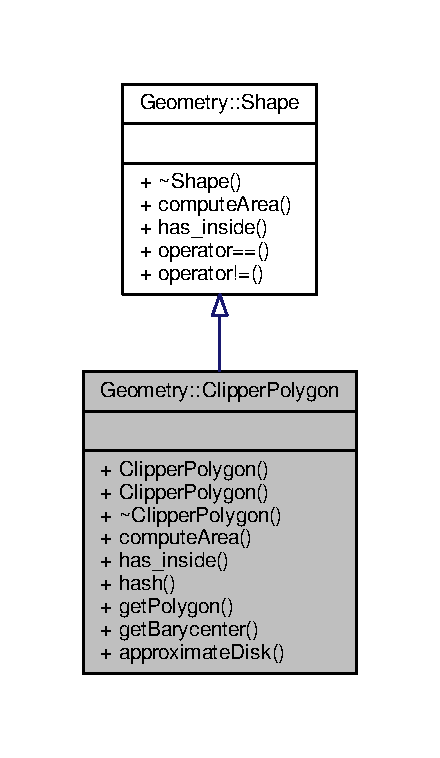
\includegraphics[width=211pt]{classGeometry_1_1ClipperPolygon__inherit__graph}
\end{center}
\end{figure}


Collaboration diagram for Geometry\+:\+:Clipper\+Polygon\+:\nopagebreak
\begin{figure}[H]
\begin{center}
\leavevmode
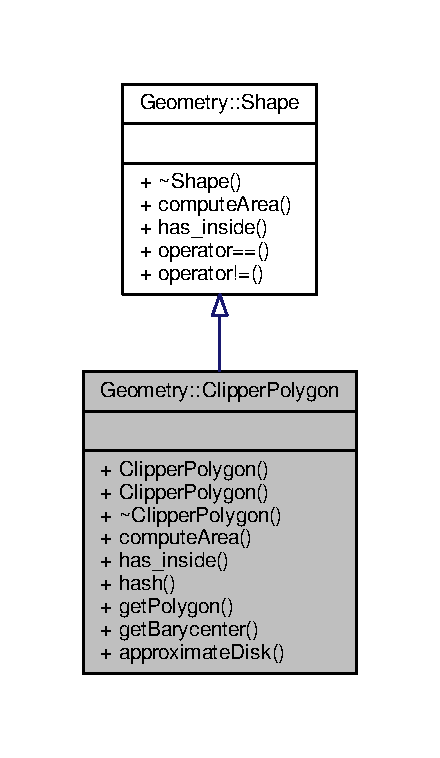
\includegraphics[width=211pt]{classGeometry_1_1ClipperPolygon__coll__graph}
\end{center}
\end{figure}
\subsection*{Public Member Functions}
\begin{DoxyCompactItemize}
\item 
\hyperlink{classGeometry_1_1ClipperPolygon_a8bb6fe04895b246e3acd28aa41158f09}{Clipper\+Polygon} (std\+::vector$<$ \hyperlink{classGeometry_1_1Point2D}{Point2\+D} $>$ \&vertices)
\item 
\hyperlink{classGeometry_1_1ClipperPolygon_a80bebeb5652e9ddd9e6582c1c023b1d6}{Clipper\+Polygon} (Clipper\+Lib\+::\+Path polygon)
\item 
\hyperlink{classGeometry_1_1ClipperPolygon_a5d266f89ec4621b9e3a4b0ea498da328}{$\sim$\+Clipper\+Polygon} () override=default
\item 
double \hyperlink{classGeometry_1_1ClipperPolygon_a452292446e85bf39afc64350180a289a}{compute\+Area} () const override
\item 
bool \hyperlink{classGeometry_1_1ClipperPolygon_a8e863b1d54c4ccc8c9d84bcccbbb137f}{has\+\_\+inside} (\hyperlink{classGeometry_1_1Point2D}{Point2\+D} p) const override
\item 
const Clipper\+Lib\+::\+Path \& \hyperlink{classGeometry_1_1ClipperPolygon_ac1528fc32d76cb7a970e3649a53ec5ef}{get\+Polygon} () const 
\end{DoxyCompactItemize}
\subsection*{Friends}
\begin{DoxyCompactItemize}
\item 
std\+::ostream \& \hyperlink{classGeometry_1_1ClipperPolygon_a005884b33ba9eeb4cf5d3fd3d02ac4bb}{operator$<$$<$} (std\+::ostream \&os, const \hyperlink{classGeometry_1_1ClipperPolygon}{Clipper\+Polygon} \&polygon)
\end{DoxyCompactItemize}


\subsection{Constructor \& Destructor Documentation}
\hypertarget{classGeometry_1_1ClipperPolygon_a8bb6fe04895b246e3acd28aa41158f09}{}\index{Geometry\+::\+Clipper\+Polygon@{Geometry\+::\+Clipper\+Polygon}!Clipper\+Polygon@{Clipper\+Polygon}}
\index{Clipper\+Polygon@{Clipper\+Polygon}!Geometry\+::\+Clipper\+Polygon@{Geometry\+::\+Clipper\+Polygon}}
\subsubsection[{Clipper\+Polygon}]{\setlength{\rightskip}{0pt plus 5cm}Geometry\+::\+Clipper\+Polygon\+::\+Clipper\+Polygon (
\begin{DoxyParamCaption}
\item[{std\+::vector$<$ {\bf Point2\+D} $>$ \&}]{vertices}
\end{DoxyParamCaption}
)\hspace{0.3cm}{\ttfamily [explicit]}}\label{classGeometry_1_1ClipperPolygon_a8bb6fe04895b246e3acd28aa41158f09}
\hypertarget{classGeometry_1_1ClipperPolygon_a80bebeb5652e9ddd9e6582c1c023b1d6}{}\index{Geometry\+::\+Clipper\+Polygon@{Geometry\+::\+Clipper\+Polygon}!Clipper\+Polygon@{Clipper\+Polygon}}
\index{Clipper\+Polygon@{Clipper\+Polygon}!Geometry\+::\+Clipper\+Polygon@{Geometry\+::\+Clipper\+Polygon}}
\subsubsection[{Clipper\+Polygon}]{\setlength{\rightskip}{0pt plus 5cm}Geometry\+::\+Clipper\+Polygon\+::\+Clipper\+Polygon (
\begin{DoxyParamCaption}
\item[{Clipper\+Lib\+::\+Path}]{polygon}
\end{DoxyParamCaption}
)\hspace{0.3cm}{\ttfamily [explicit]}}\label{classGeometry_1_1ClipperPolygon_a80bebeb5652e9ddd9e6582c1c023b1d6}
\hypertarget{classGeometry_1_1ClipperPolygon_a5d266f89ec4621b9e3a4b0ea498da328}{}\index{Geometry\+::\+Clipper\+Polygon@{Geometry\+::\+Clipper\+Polygon}!````~Clipper\+Polygon@{$\sim$\+Clipper\+Polygon}}
\index{````~Clipper\+Polygon@{$\sim$\+Clipper\+Polygon}!Geometry\+::\+Clipper\+Polygon@{Geometry\+::\+Clipper\+Polygon}}
\subsubsection[{$\sim$\+Clipper\+Polygon}]{\setlength{\rightskip}{0pt plus 5cm}Geometry\+::\+Clipper\+Polygon\+::$\sim$\+Clipper\+Polygon (
\begin{DoxyParamCaption}
{}
\end{DoxyParamCaption}
)\hspace{0.3cm}{\ttfamily [override]}, {\ttfamily [default]}}\label{classGeometry_1_1ClipperPolygon_a5d266f89ec4621b9e3a4b0ea498da328}


\subsection{Member Function Documentation}
\hypertarget{classGeometry_1_1ClipperPolygon_a452292446e85bf39afc64350180a289a}{}\index{Geometry\+::\+Clipper\+Polygon@{Geometry\+::\+Clipper\+Polygon}!compute\+Area@{compute\+Area}}
\index{compute\+Area@{compute\+Area}!Geometry\+::\+Clipper\+Polygon@{Geometry\+::\+Clipper\+Polygon}}
\subsubsection[{compute\+Area}]{\setlength{\rightskip}{0pt plus 5cm}double Geometry\+::\+Clipper\+Polygon\+::compute\+Area (
\begin{DoxyParamCaption}
{}
\end{DoxyParamCaption}
) const\hspace{0.3cm}{\ttfamily [override]}, {\ttfamily [virtual]}}\label{classGeometry_1_1ClipperPolygon_a452292446e85bf39afc64350180a289a}


Implements \hyperlink{classGeometry_1_1Shape_ad0fb97e79dc8c171482bc14726ad8ce7}{Geometry\+::\+Shape}.

\hypertarget{classGeometry_1_1ClipperPolygon_ac1528fc32d76cb7a970e3649a53ec5ef}{}\index{Geometry\+::\+Clipper\+Polygon@{Geometry\+::\+Clipper\+Polygon}!get\+Polygon@{get\+Polygon}}
\index{get\+Polygon@{get\+Polygon}!Geometry\+::\+Clipper\+Polygon@{Geometry\+::\+Clipper\+Polygon}}
\subsubsection[{get\+Polygon}]{\setlength{\rightskip}{0pt plus 5cm}const Clipper\+Lib\+::\+Path \& Geometry\+::\+Clipper\+Polygon\+::get\+Polygon (
\begin{DoxyParamCaption}
{}
\end{DoxyParamCaption}
) const}\label{classGeometry_1_1ClipperPolygon_ac1528fc32d76cb7a970e3649a53ec5ef}
\hypertarget{classGeometry_1_1ClipperPolygon_a8e863b1d54c4ccc8c9d84bcccbbb137f}{}\index{Geometry\+::\+Clipper\+Polygon@{Geometry\+::\+Clipper\+Polygon}!has\+\_\+inside@{has\+\_\+inside}}
\index{has\+\_\+inside@{has\+\_\+inside}!Geometry\+::\+Clipper\+Polygon@{Geometry\+::\+Clipper\+Polygon}}
\subsubsection[{has\+\_\+inside}]{\setlength{\rightskip}{0pt plus 5cm}bool Geometry\+::\+Clipper\+Polygon\+::has\+\_\+inside (
\begin{DoxyParamCaption}
\item[{{\bf Point2\+D}}]{p}
\end{DoxyParamCaption}
) const\hspace{0.3cm}{\ttfamily [override]}, {\ttfamily [virtual]}}\label{classGeometry_1_1ClipperPolygon_a8e863b1d54c4ccc8c9d84bcccbbb137f}


Implements \hyperlink{classGeometry_1_1Shape_a2e1341ab60671a72a96bca2238cd38f0}{Geometry\+::\+Shape}.



\subsection{Friends And Related Function Documentation}
\hypertarget{classGeometry_1_1ClipperPolygon_a005884b33ba9eeb4cf5d3fd3d02ac4bb}{}\index{Geometry\+::\+Clipper\+Polygon@{Geometry\+::\+Clipper\+Polygon}!operator$<$$<$@{operator$<$$<$}}
\index{operator$<$$<$@{operator$<$$<$}!Geometry\+::\+Clipper\+Polygon@{Geometry\+::\+Clipper\+Polygon}}
\subsubsection[{operator$<$$<$}]{\setlength{\rightskip}{0pt plus 5cm}std\+::ostream\& operator$<$$<$ (
\begin{DoxyParamCaption}
\item[{std\+::ostream \&}]{os, }
\item[{const {\bf Clipper\+Polygon} \&}]{polygon}
\end{DoxyParamCaption}
)\hspace{0.3cm}{\ttfamily [friend]}}\label{classGeometry_1_1ClipperPolygon_a005884b33ba9eeb4cf5d3fd3d02ac4bb}


The documentation for this class was generated from the following files\+:\begin{DoxyCompactItemize}
\item 
geometry/\hyperlink{ClipperPolygon_8h}{Clipper\+Polygon.\+h}\item 
geometry/\hyperlink{ClipperPolygon_8cpp}{Clipper\+Polygon.\+cpp}\end{DoxyCompactItemize}

\hypertarget{classCompositeFocalElement}{}\section{Composite\+Focal\+Element Class Reference}
\label{classCompositeFocalElement}\index{Composite\+Focal\+Element@{Composite\+Focal\+Element}}


{\ttfamily \#include $<$Composite\+Focal\+Element.\+h$>$}



Inheritance diagram for Composite\+Focal\+Element\+:\nopagebreak
\begin{figure}[H]
\begin{center}
\leavevmode
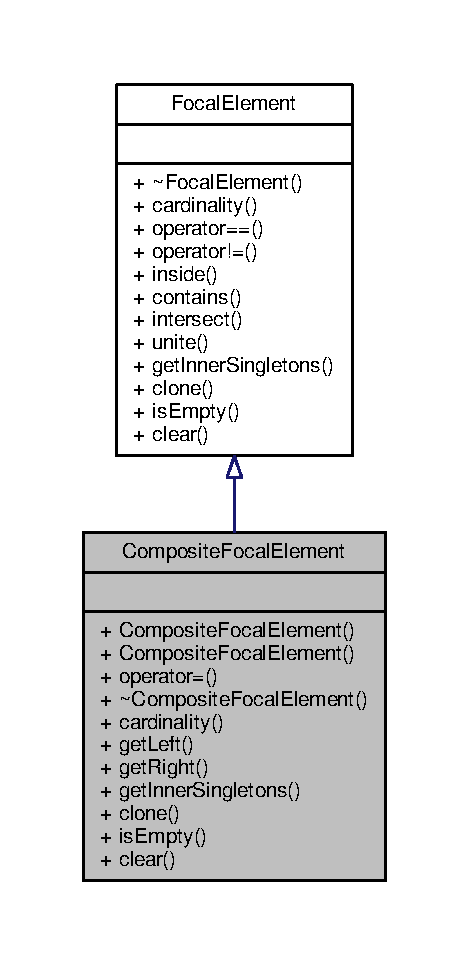
\includegraphics[width=225pt]{classCompositeFocalElement__inherit__graph}
\end{center}
\end{figure}


Collaboration diagram for Composite\+Focal\+Element\+:\nopagebreak
\begin{figure}[H]
\begin{center}
\leavevmode
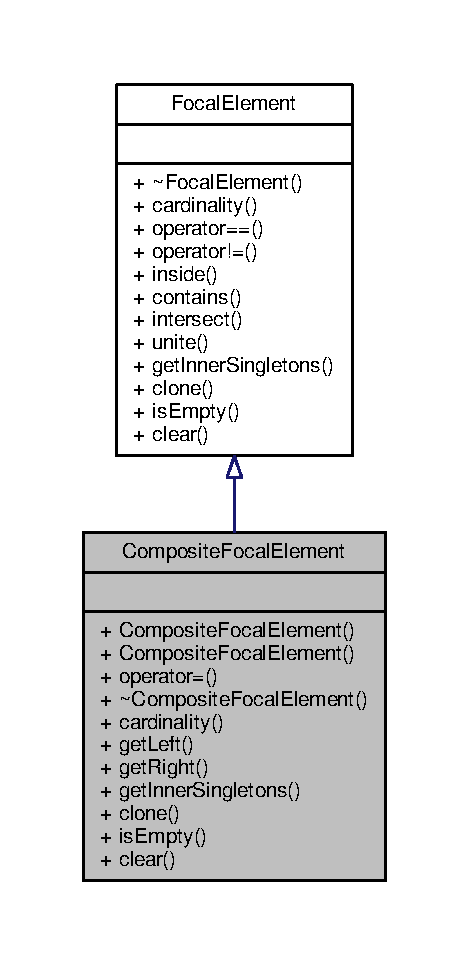
\includegraphics[width=225pt]{classCompositeFocalElement__coll__graph}
\end{center}
\end{figure}
\subsection*{Public Member Functions}
\begin{DoxyCompactItemize}
\item 
\hyperlink{classCompositeFocalElement_a5edb45a7eb4e963f8a3fe9f5e86dbcc2}{Composite\+Focal\+Element} (std\+::unique\+\_\+ptr$<$ \hyperlink{classFocalElement}{Focal\+Element} $>$ \+\_\+left, std\+::unique\+\_\+ptr$<$ \hyperlink{classFocalElement}{Focal\+Element} $>$ \+\_\+right)
\item 
\hyperlink{classCompositeFocalElement_ad7bf43cd99f64e40b1db1d02dbb69713}{Composite\+Focal\+Element} (const \hyperlink{classCompositeFocalElement}{Composite\+Focal\+Element} \&other)
\item 
\hyperlink{classCompositeFocalElement}{Composite\+Focal\+Element} \& \hyperlink{classCompositeFocalElement_a08412d0e70bab10c523baa83b6eb1937}{operator=} (const \hyperlink{classCompositeFocalElement}{Composite\+Focal\+Element} \&other)
\item 
\hyperlink{classCompositeFocalElement_a29f321b81347d8d687aca284e0507aec}{$\sim$\+Composite\+Focal\+Element} () override=default
\item 
double \hyperlink{classCompositeFocalElement_a18a671ee1759b5df42770384ace275fd}{cardinality} () const override
\item 
const std\+::unique\+\_\+ptr$<$ \hyperlink{classFocalElement}{Focal\+Element} $>$ \& \hyperlink{classCompositeFocalElement_af4e6a58bc9db40cde3446b76d91f5e57}{get\+Left} () const 
\item 
const std\+::unique\+\_\+ptr$<$ \hyperlink{classFocalElement}{Focal\+Element} $>$ \& \hyperlink{classCompositeFocalElement_aef97b94d2375742722833674a3f38a54}{get\+Right} () const 
\item 
std\+::vector$<$ std\+::unique\+\_\+ptr$<$ \hyperlink{classFocalElement}{Focal\+Element} $>$ $>$ \hyperlink{classCompositeFocalElement_aae945111cdffaaa5dc3216e439ac6ad2}{get\+Inner\+Singletons} (int step\+\_\+size=1) const override
\item 
std\+::unique\+\_\+ptr$<$ \hyperlink{classFocalElement}{Focal\+Element} $>$ \hyperlink{classCompositeFocalElement_a3ae99f9c094419664e443d650560baf4}{clone} () const override
\item 
bool \hyperlink{classCompositeFocalElement_a015e5fa735f796d4ac38aec2e332b49a}{is\+Empty} () const override
\item 
void \hyperlink{classCompositeFocalElement_a010c40507f9c45da7327f0418ea32b53}{clear} () override
\end{DoxyCompactItemize}


\subsection{Constructor \& Destructor Documentation}
\hypertarget{classCompositeFocalElement_a5edb45a7eb4e963f8a3fe9f5e86dbcc2}{}\index{Composite\+Focal\+Element@{Composite\+Focal\+Element}!Composite\+Focal\+Element@{Composite\+Focal\+Element}}
\index{Composite\+Focal\+Element@{Composite\+Focal\+Element}!Composite\+Focal\+Element@{Composite\+Focal\+Element}}
\subsubsection[{Composite\+Focal\+Element}]{\setlength{\rightskip}{0pt plus 5cm}Composite\+Focal\+Element\+::\+Composite\+Focal\+Element (
\begin{DoxyParamCaption}
\item[{std\+::unique\+\_\+ptr$<$ {\bf Focal\+Element} $>$}]{\+\_\+left, }
\item[{std\+::unique\+\_\+ptr$<$ {\bf Focal\+Element} $>$}]{\+\_\+right}
\end{DoxyParamCaption}
)\hspace{0.3cm}{\ttfamily [inline]}, {\ttfamily [explicit]}}\label{classCompositeFocalElement_a5edb45a7eb4e963f8a3fe9f5e86dbcc2}
\hypertarget{classCompositeFocalElement_ad7bf43cd99f64e40b1db1d02dbb69713}{}\index{Composite\+Focal\+Element@{Composite\+Focal\+Element}!Composite\+Focal\+Element@{Composite\+Focal\+Element}}
\index{Composite\+Focal\+Element@{Composite\+Focal\+Element}!Composite\+Focal\+Element@{Composite\+Focal\+Element}}
\subsubsection[{Composite\+Focal\+Element}]{\setlength{\rightskip}{0pt plus 5cm}Composite\+Focal\+Element\+::\+Composite\+Focal\+Element (
\begin{DoxyParamCaption}
\item[{const {\bf Composite\+Focal\+Element} \&}]{other}
\end{DoxyParamCaption}
)}\label{classCompositeFocalElement_ad7bf43cd99f64e40b1db1d02dbb69713}
\hypertarget{classCompositeFocalElement_a29f321b81347d8d687aca284e0507aec}{}\index{Composite\+Focal\+Element@{Composite\+Focal\+Element}!````~Composite\+Focal\+Element@{$\sim$\+Composite\+Focal\+Element}}
\index{````~Composite\+Focal\+Element@{$\sim$\+Composite\+Focal\+Element}!Composite\+Focal\+Element@{Composite\+Focal\+Element}}
\subsubsection[{$\sim$\+Composite\+Focal\+Element}]{\setlength{\rightskip}{0pt plus 5cm}Composite\+Focal\+Element\+::$\sim$\+Composite\+Focal\+Element (
\begin{DoxyParamCaption}
{}
\end{DoxyParamCaption}
)\hspace{0.3cm}{\ttfamily [override]}, {\ttfamily [default]}}\label{classCompositeFocalElement_a29f321b81347d8d687aca284e0507aec}


\subsection{Member Function Documentation}
\hypertarget{classCompositeFocalElement_a18a671ee1759b5df42770384ace275fd}{}\index{Composite\+Focal\+Element@{Composite\+Focal\+Element}!cardinality@{cardinality}}
\index{cardinality@{cardinality}!Composite\+Focal\+Element@{Composite\+Focal\+Element}}
\subsubsection[{cardinality}]{\setlength{\rightskip}{0pt plus 5cm}double Composite\+Focal\+Element\+::cardinality (
\begin{DoxyParamCaption}
{}
\end{DoxyParamCaption}
) const\hspace{0.3cm}{\ttfamily [override]}, {\ttfamily [virtual]}}\label{classCompositeFocalElement_a18a671ee1759b5df42770384ace275fd}


Implements \hyperlink{classFocalElement_a4ab1bbd0875e6e7ce2d7fe152e6a1639}{Focal\+Element}.

\hypertarget{classCompositeFocalElement_a010c40507f9c45da7327f0418ea32b53}{}\index{Composite\+Focal\+Element@{Composite\+Focal\+Element}!clear@{clear}}
\index{clear@{clear}!Composite\+Focal\+Element@{Composite\+Focal\+Element}}
\subsubsection[{clear}]{\setlength{\rightskip}{0pt plus 5cm}void Composite\+Focal\+Element\+::clear (
\begin{DoxyParamCaption}
{}
\end{DoxyParamCaption}
)\hspace{0.3cm}{\ttfamily [override]}, {\ttfamily [virtual]}}\label{classCompositeFocalElement_a010c40507f9c45da7327f0418ea32b53}


Implements \hyperlink{classFocalElement_a635cb4afffa2dc69cf9fc9ff94a6d90f}{Focal\+Element}.

\hypertarget{classCompositeFocalElement_a3ae99f9c094419664e443d650560baf4}{}\index{Composite\+Focal\+Element@{Composite\+Focal\+Element}!clone@{clone}}
\index{clone@{clone}!Composite\+Focal\+Element@{Composite\+Focal\+Element}}
\subsubsection[{clone}]{\setlength{\rightskip}{0pt plus 5cm}std\+::unique\+\_\+ptr$<$ {\bf Focal\+Element} $>$ Composite\+Focal\+Element\+::clone (
\begin{DoxyParamCaption}
{}
\end{DoxyParamCaption}
) const\hspace{0.3cm}{\ttfamily [override]}, {\ttfamily [virtual]}}\label{classCompositeFocalElement_a3ae99f9c094419664e443d650560baf4}


Implements \hyperlink{classFocalElement_a21697fbbbcb144c18fa7b4ecae5e6145}{Focal\+Element}.

\hypertarget{classCompositeFocalElement_aae945111cdffaaa5dc3216e439ac6ad2}{}\index{Composite\+Focal\+Element@{Composite\+Focal\+Element}!get\+Inner\+Singletons@{get\+Inner\+Singletons}}
\index{get\+Inner\+Singletons@{get\+Inner\+Singletons}!Composite\+Focal\+Element@{Composite\+Focal\+Element}}
\subsubsection[{get\+Inner\+Singletons}]{\setlength{\rightskip}{0pt plus 5cm}std\+::vector$<$ std\+::unique\+\_\+ptr$<$ {\bf Focal\+Element} $>$ $>$ Composite\+Focal\+Element\+::get\+Inner\+Singletons (
\begin{DoxyParamCaption}
\item[{int}]{step\+\_\+size = {\ttfamily 1}}
\end{DoxyParamCaption}
) const\hspace{0.3cm}{\ttfamily [override]}, {\ttfamily [virtual]}}\label{classCompositeFocalElement_aae945111cdffaaa5dc3216e439ac6ad2}


Implements \hyperlink{classFocalElement_ac615e960ea64a4bdc0f442135f6069e2}{Focal\+Element}.

\hypertarget{classCompositeFocalElement_af4e6a58bc9db40cde3446b76d91f5e57}{}\index{Composite\+Focal\+Element@{Composite\+Focal\+Element}!get\+Left@{get\+Left}}
\index{get\+Left@{get\+Left}!Composite\+Focal\+Element@{Composite\+Focal\+Element}}
\subsubsection[{get\+Left}]{\setlength{\rightskip}{0pt plus 5cm}const std\+::unique\+\_\+ptr$<$ {\bf Focal\+Element} $>$ \& Composite\+Focal\+Element\+::get\+Left (
\begin{DoxyParamCaption}
{}
\end{DoxyParamCaption}
) const}\label{classCompositeFocalElement_af4e6a58bc9db40cde3446b76d91f5e57}
\hypertarget{classCompositeFocalElement_aef97b94d2375742722833674a3f38a54}{}\index{Composite\+Focal\+Element@{Composite\+Focal\+Element}!get\+Right@{get\+Right}}
\index{get\+Right@{get\+Right}!Composite\+Focal\+Element@{Composite\+Focal\+Element}}
\subsubsection[{get\+Right}]{\setlength{\rightskip}{0pt plus 5cm}const std\+::unique\+\_\+ptr$<$ {\bf Focal\+Element} $>$ \& Composite\+Focal\+Element\+::get\+Right (
\begin{DoxyParamCaption}
{}
\end{DoxyParamCaption}
) const}\label{classCompositeFocalElement_aef97b94d2375742722833674a3f38a54}
\hypertarget{classCompositeFocalElement_a015e5fa735f796d4ac38aec2e332b49a}{}\index{Composite\+Focal\+Element@{Composite\+Focal\+Element}!is\+Empty@{is\+Empty}}
\index{is\+Empty@{is\+Empty}!Composite\+Focal\+Element@{Composite\+Focal\+Element}}
\subsubsection[{is\+Empty}]{\setlength{\rightskip}{0pt plus 5cm}bool Composite\+Focal\+Element\+::is\+Empty (
\begin{DoxyParamCaption}
{}
\end{DoxyParamCaption}
) const\hspace{0.3cm}{\ttfamily [override]}, {\ttfamily [virtual]}}\label{classCompositeFocalElement_a015e5fa735f796d4ac38aec2e332b49a}


Implements \hyperlink{classFocalElement_aed131a65fdfc885019f9bf8f1d454508}{Focal\+Element}.

\hypertarget{classCompositeFocalElement_a08412d0e70bab10c523baa83b6eb1937}{}\index{Composite\+Focal\+Element@{Composite\+Focal\+Element}!operator=@{operator=}}
\index{operator=@{operator=}!Composite\+Focal\+Element@{Composite\+Focal\+Element}}
\subsubsection[{operator=}]{\setlength{\rightskip}{0pt plus 5cm}{\bf Composite\+Focal\+Element} \& Composite\+Focal\+Element\+::operator= (
\begin{DoxyParamCaption}
\item[{const {\bf Composite\+Focal\+Element} \&}]{other}
\end{DoxyParamCaption}
)}\label{classCompositeFocalElement_a08412d0e70bab10c523baa83b6eb1937}


The documentation for this class was generated from the following files\+:\begin{DoxyCompactItemize}
\item 
focal\+\_\+elements/\hyperlink{CompositeFocalElement_8h}{Composite\+Focal\+Element.\+h}\item 
focal\+\_\+elements/\hyperlink{CompositeFocalElement_8cpp}{Composite\+Focal\+Element.\+cpp}\end{DoxyCompactItemize}

\hypertarget{classConstructorArgumentsError}{}\section{Constructor\+Arguments\+Error Class Reference}
\label{classConstructorArgumentsError}\index{Constructor\+Arguments\+Error@{Constructor\+Arguments\+Error}}


{\ttfamily \#include $<$Constructor\+Arguments\+Error.\+h$>$}



Inheritance diagram for Constructor\+Arguments\+Error\+:\nopagebreak
\begin{figure}[H]
\begin{center}
\leavevmode
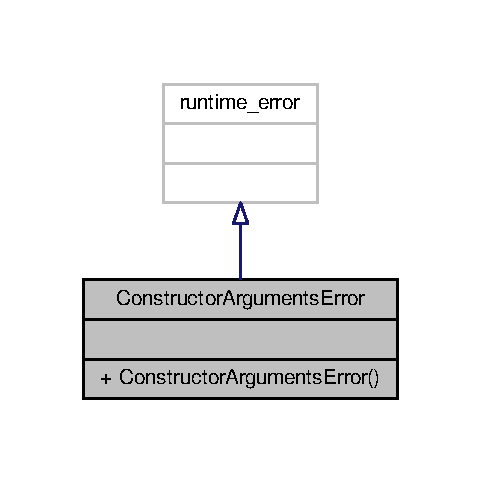
\includegraphics[width=231pt]{classConstructorArgumentsError__inherit__graph}
\end{center}
\end{figure}


Collaboration diagram for Constructor\+Arguments\+Error\+:\nopagebreak
\begin{figure}[H]
\begin{center}
\leavevmode
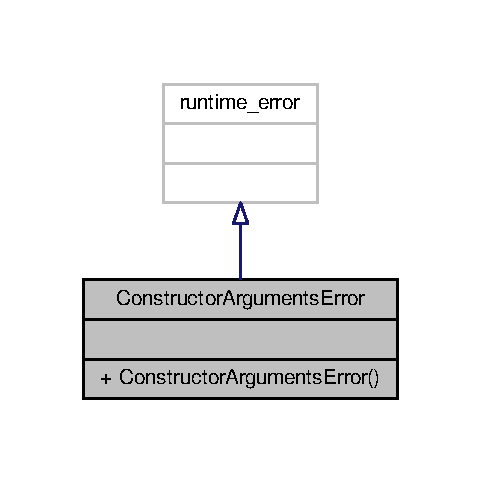
\includegraphics[width=231pt]{classConstructorArgumentsError__coll__graph}
\end{center}
\end{figure}
\subsection*{Public Member Functions}
\begin{DoxyCompactItemize}
\item 
\hyperlink{classConstructorArgumentsError_a6150c7b431f6c58babc9c280e26497a3}{Constructor\+Arguments\+Error} (const char $\ast$msg)
\end{DoxyCompactItemize}


\subsection{Constructor \& Destructor Documentation}
\hypertarget{classConstructorArgumentsError_a6150c7b431f6c58babc9c280e26497a3}{}\index{Constructor\+Arguments\+Error@{Constructor\+Arguments\+Error}!Constructor\+Arguments\+Error@{Constructor\+Arguments\+Error}}
\index{Constructor\+Arguments\+Error@{Constructor\+Arguments\+Error}!Constructor\+Arguments\+Error@{Constructor\+Arguments\+Error}}
\subsubsection[{Constructor\+Arguments\+Error}]{\setlength{\rightskip}{0pt plus 5cm}Constructor\+Arguments\+Error\+::\+Constructor\+Arguments\+Error (
\begin{DoxyParamCaption}
\item[{const char $\ast$}]{msg}
\end{DoxyParamCaption}
)\hspace{0.3cm}{\ttfamily [inline]}, {\ttfamily [explicit]}}\label{classConstructorArgumentsError_a6150c7b431f6c58babc9c280e26497a3}


The documentation for this class was generated from the following file\+:\begin{DoxyCompactItemize}
\item 
errors/\hyperlink{ConstructorArgumentsError_8h}{Constructor\+Arguments\+Error.\+h}\end{DoxyCompactItemize}

\hypertarget{classDefaultFocalElementContainerDispatcher}{}\section{Default\+Focal\+Element\+Container\+Dispatcher Class Reference}
\label{classDefaultFocalElementContainerDispatcher}\index{Default\+Focal\+Element\+Container\+Dispatcher@{Default\+Focal\+Element\+Container\+Dispatcher}}


The default dispatcher for \hyperlink{classFocalElementContainer}{Focal\+Element\+Container}.  




{\ttfamily \#include $<$Default\+Focal\+Element\+Container\+Dispatcher.\+h$>$}



Inheritance diagram for Default\+Focal\+Element\+Container\+Dispatcher\+:\nopagebreak
\begin{figure}[H]
\begin{center}
\leavevmode
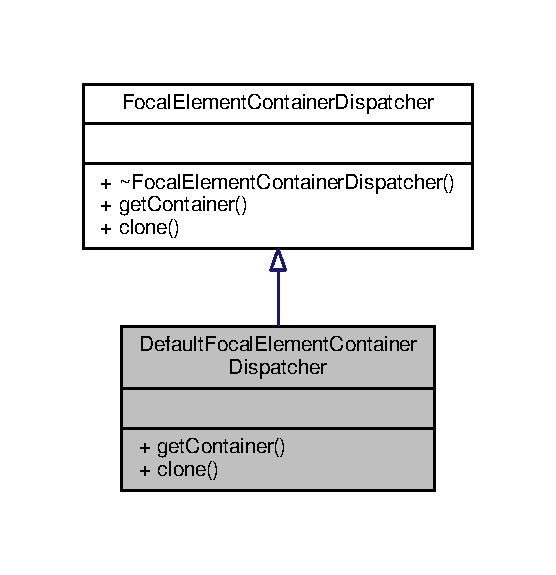
\includegraphics[width=267pt]{classDefaultFocalElementContainerDispatcher__inherit__graph}
\end{center}
\end{figure}


Collaboration diagram for Default\+Focal\+Element\+Container\+Dispatcher\+:\nopagebreak
\begin{figure}[H]
\begin{center}
\leavevmode
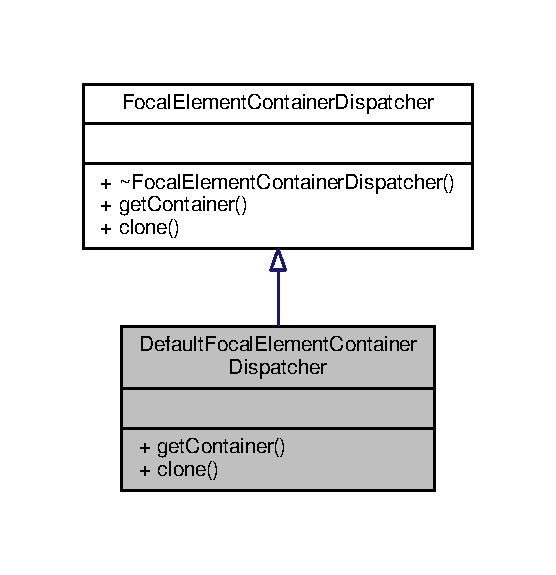
\includegraphics[width=267pt]{classDefaultFocalElementContainerDispatcher__coll__graph}
\end{center}
\end{figure}
\subsection*{Public Member Functions}
\begin{DoxyCompactItemize}
\item 
std\+::unique\+\_\+ptr$<$ \hyperlink{classFocalElementContainer}{Focal\+Element\+Container} $>$ \hyperlink{classDefaultFocalElementContainerDispatcher_a3e2952b8397e02d4ca917e257471781e}{get\+Container} (const \hyperlink{classFocalElement}{Focal\+Element} \&el) override
\begin{DoxyCompactList}\small\item\em Get the container given the \hyperlink{classFocalElement}{Focal\+Element} type. \end{DoxyCompactList}\item 
std\+::unique\+\_\+ptr$<$ \hyperlink{classFocalElementContainerDispatcher}{Focal\+Element\+Container\+Dispatcher} $>$ \hyperlink{classDefaultFocalElementContainerDispatcher_ac3908e561d7116fdf5b9c6ec9c2b6fdb}{clone} () override
\begin{DoxyCompactList}\small\item\em Clone method. \end{DoxyCompactList}\end{DoxyCompactItemize}


\subsection{Detailed Description}
The default dispatcher for \hyperlink{classFocalElementContainer}{Focal\+Element\+Container}. 

Error in the arguments of a constructor method.

It distinguishes between generic and hashable \hyperlink{classFocalElement}{Focal\+Element}. 

\subsection{Member Function Documentation}
\hypertarget{classDefaultFocalElementContainerDispatcher_ac3908e561d7116fdf5b9c6ec9c2b6fdb}{}\index{Default\+Focal\+Element\+Container\+Dispatcher@{Default\+Focal\+Element\+Container\+Dispatcher}!clone@{clone}}
\index{clone@{clone}!Default\+Focal\+Element\+Container\+Dispatcher@{Default\+Focal\+Element\+Container\+Dispatcher}}
\subsubsection[{clone}]{\setlength{\rightskip}{0pt plus 5cm}std\+::unique\+\_\+ptr$<$ {\bf Focal\+Element\+Container\+Dispatcher} $>$ Default\+Focal\+Element\+Container\+Dispatcher\+::clone (
\begin{DoxyParamCaption}
{}
\end{DoxyParamCaption}
)\hspace{0.3cm}{\ttfamily [override]}, {\ttfamily [virtual]}}\label{classDefaultFocalElementContainerDispatcher_ac3908e561d7116fdf5b9c6ec9c2b6fdb}


Clone method. 

\begin{DoxyReturn}{Returns}
A copy of the \hyperlink{classFocalElementContainerDispatcher}{Focal\+Element\+Container\+Dispatcher} object. 
\end{DoxyReturn}


Implements \hyperlink{classFocalElementContainerDispatcher_a710d8bb32947cde2ad5c5e914f33b767}{Focal\+Element\+Container\+Dispatcher}.

\hypertarget{classDefaultFocalElementContainerDispatcher_a3e2952b8397e02d4ca917e257471781e}{}\index{Default\+Focal\+Element\+Container\+Dispatcher@{Default\+Focal\+Element\+Container\+Dispatcher}!get\+Container@{get\+Container}}
\index{get\+Container@{get\+Container}!Default\+Focal\+Element\+Container\+Dispatcher@{Default\+Focal\+Element\+Container\+Dispatcher}}
\subsubsection[{get\+Container}]{\setlength{\rightskip}{0pt plus 5cm}std\+::unique\+\_\+ptr$<$ {\bf Focal\+Element\+Container} $>$ Default\+Focal\+Element\+Container\+Dispatcher\+::get\+Container (
\begin{DoxyParamCaption}
\item[{const {\bf Focal\+Element} \&}]{el}
\end{DoxyParamCaption}
)\hspace{0.3cm}{\ttfamily [override]}, {\ttfamily [virtual]}}\label{classDefaultFocalElementContainerDispatcher_a3e2952b8397e02d4ca917e257471781e}


Get the container given the \hyperlink{classFocalElement}{Focal\+Element} type. 


\begin{DoxyParams}{Parameters}
{\em el} & Target \hyperlink{classFocalElement}{Focal\+Element} \\
\hline
\end{DoxyParams}
\begin{DoxyReturn}{Returns}
The related \hyperlink{classFocalElementContainer}{Focal\+Element\+Container} 
\end{DoxyReturn}


Implements \hyperlink{classFocalElementContainerDispatcher_af429ae69c47220d55b30cf7e41ee6928}{Focal\+Element\+Container\+Dispatcher}.



The documentation for this class was generated from the following files\+:\begin{DoxyCompactItemize}
\item 
builders/\hyperlink{DefaultFocalElementContainerDispatcher_8h}{Default\+Focal\+Element\+Container\+Dispatcher.\+h}\item 
builders/\hyperlink{DefaultFocalElementContainerDispatcher_8cpp}{Default\+Focal\+Element\+Container\+Dispatcher.\+cpp}\end{DoxyCompactItemize}

\hypertarget{classEigenFE_1_1EigenMat2DFocalElement}{}\section{Eigen\+F\+E\+:\+:Eigen\+Mat2\+D\+Focal\+Element Class Reference}
\label{classEigenFE_1_1EigenMat2DFocalElement}\index{Eigen\+F\+E\+::\+Eigen\+Mat2\+D\+Focal\+Element@{Eigen\+F\+E\+::\+Eigen\+Mat2\+D\+Focal\+Element}}


{\ttfamily \#include $<$Eigen\+Mat2\+D\+Focal\+Element.\+h$>$}



Inheritance diagram for Eigen\+F\+E\+:\+:Eigen\+Mat2\+D\+Focal\+Element\+:\nopagebreak
\begin{figure}[H]
\begin{center}
\leavevmode
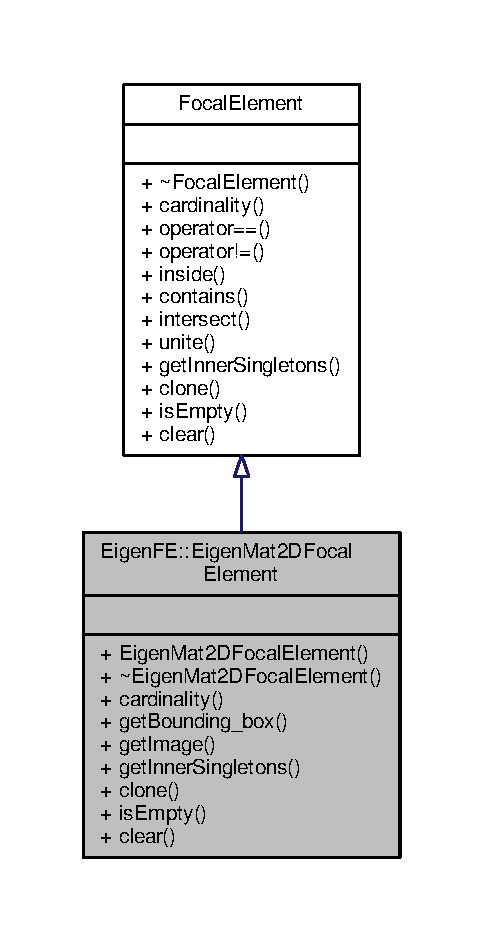
\includegraphics[width=232pt]{classEigenFE_1_1EigenMat2DFocalElement__inherit__graph}
\end{center}
\end{figure}


Collaboration diagram for Eigen\+F\+E\+:\+:Eigen\+Mat2\+D\+Focal\+Element\+:\nopagebreak
\begin{figure}[H]
\begin{center}
\leavevmode
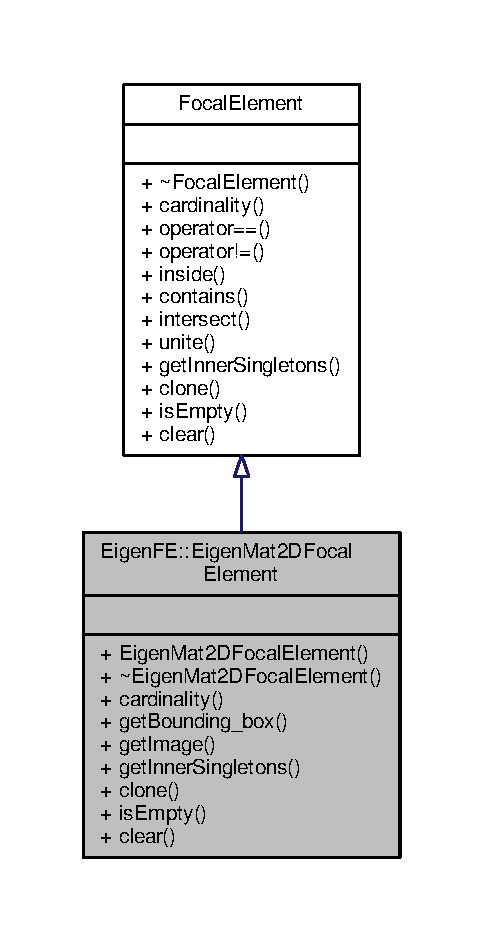
\includegraphics[width=232pt]{classEigenFE_1_1EigenMat2DFocalElement__coll__graph}
\end{center}
\end{figure}
\subsection*{Public Member Functions}
\begin{DoxyCompactItemize}
\item 
\hyperlink{classEigenFE_1_1EigenMat2DFocalElement_ab1e04c916b081d4ac8f65c071619f2ae}{Eigen\+Mat2\+D\+Focal\+Element} (const \hyperlink{classGeometry_1_1Rectangle}{Geometry\+::\+Rectangle} \&bounding\+\_\+box, const \hyperlink{namespaceEigenFE_a478c1c0c93aef88b798e7c38a9c65d59}{Matrix\+Xb} \&image)
\item 
\hyperlink{classEigenFE_1_1EigenMat2DFocalElement_a8d16fd73bfb48a9cce07e6e8ea5cb83d}{$\sim$\+Eigen\+Mat2\+D\+Focal\+Element} () override=default
\item 
double \hyperlink{classEigenFE_1_1EigenMat2DFocalElement_ac19a1317772f2946bd8956cb084a3a1b}{cardinality} () const override
\item 
const \hyperlink{classGeometry_1_1Rectangle}{Geometry\+::\+Rectangle} \& \hyperlink{classEigenFE_1_1EigenMat2DFocalElement_a87b3b927b9b669c4120efb6c271a14d6}{get\+Bounding\+\_\+box} () const 
\item 
const \hyperlink{namespaceEigenFE_a478c1c0c93aef88b798e7c38a9c65d59}{Matrix\+Xb} \& \hyperlink{classEigenFE_1_1EigenMat2DFocalElement_a50caa5018108e7c376c313c8c301165d}{get\+Image} () const 
\item 
std\+::vector$<$ std\+::unique\+\_\+ptr$<$ \hyperlink{classFocalElement}{Focal\+Element} $>$ $>$ \hyperlink{classEigenFE_1_1EigenMat2DFocalElement_a02348604649107935c95106b1fb18a06}{get\+Inner\+Singletons} (int step\+\_\+size=1) const override
\item 
std\+::unique\+\_\+ptr$<$ \hyperlink{classFocalElement}{Focal\+Element} $>$ \hyperlink{classEigenFE_1_1EigenMat2DFocalElement_a7b11a9c1a340338ddc0502c04c3ebb50}{clone} () const override
\item 
bool \hyperlink{classEigenFE_1_1EigenMat2DFocalElement_af0b7bcf11590355059f49c59c51aea3f}{is\+Empty} () const override
\item 
void \hyperlink{classEigenFE_1_1EigenMat2DFocalElement_a32f67417ea35cb7d330d8ca27472c863}{clear} () override
\end{DoxyCompactItemize}


\subsection{Constructor \& Destructor Documentation}
\hypertarget{classEigenFE_1_1EigenMat2DFocalElement_ab1e04c916b081d4ac8f65c071619f2ae}{}\index{Eigen\+F\+E\+::\+Eigen\+Mat2\+D\+Focal\+Element@{Eigen\+F\+E\+::\+Eigen\+Mat2\+D\+Focal\+Element}!Eigen\+Mat2\+D\+Focal\+Element@{Eigen\+Mat2\+D\+Focal\+Element}}
\index{Eigen\+Mat2\+D\+Focal\+Element@{Eigen\+Mat2\+D\+Focal\+Element}!Eigen\+F\+E\+::\+Eigen\+Mat2\+D\+Focal\+Element@{Eigen\+F\+E\+::\+Eigen\+Mat2\+D\+Focal\+Element}}
\subsubsection[{Eigen\+Mat2\+D\+Focal\+Element}]{\setlength{\rightskip}{0pt plus 5cm}Eigen\+F\+E\+::\+Eigen\+Mat2\+D\+Focal\+Element\+::\+Eigen\+Mat2\+D\+Focal\+Element (
\begin{DoxyParamCaption}
\item[{const {\bf Geometry\+::\+Rectangle} \&}]{bounding\+\_\+box, }
\item[{const {\bf Matrix\+Xb} \&}]{image}
\end{DoxyParamCaption}
)}\label{classEigenFE_1_1EigenMat2DFocalElement_ab1e04c916b081d4ac8f65c071619f2ae}
\hypertarget{classEigenFE_1_1EigenMat2DFocalElement_a8d16fd73bfb48a9cce07e6e8ea5cb83d}{}\index{Eigen\+F\+E\+::\+Eigen\+Mat2\+D\+Focal\+Element@{Eigen\+F\+E\+::\+Eigen\+Mat2\+D\+Focal\+Element}!````~Eigen\+Mat2\+D\+Focal\+Element@{$\sim$\+Eigen\+Mat2\+D\+Focal\+Element}}
\index{````~Eigen\+Mat2\+D\+Focal\+Element@{$\sim$\+Eigen\+Mat2\+D\+Focal\+Element}!Eigen\+F\+E\+::\+Eigen\+Mat2\+D\+Focal\+Element@{Eigen\+F\+E\+::\+Eigen\+Mat2\+D\+Focal\+Element}}
\subsubsection[{$\sim$\+Eigen\+Mat2\+D\+Focal\+Element}]{\setlength{\rightskip}{0pt plus 5cm}Eigen\+F\+E\+::\+Eigen\+Mat2\+D\+Focal\+Element\+::$\sim$\+Eigen\+Mat2\+D\+Focal\+Element (
\begin{DoxyParamCaption}
{}
\end{DoxyParamCaption}
)\hspace{0.3cm}{\ttfamily [override]}, {\ttfamily [default]}}\label{classEigenFE_1_1EigenMat2DFocalElement_a8d16fd73bfb48a9cce07e6e8ea5cb83d}


\subsection{Member Function Documentation}
\hypertarget{classEigenFE_1_1EigenMat2DFocalElement_ac19a1317772f2946bd8956cb084a3a1b}{}\index{Eigen\+F\+E\+::\+Eigen\+Mat2\+D\+Focal\+Element@{Eigen\+F\+E\+::\+Eigen\+Mat2\+D\+Focal\+Element}!cardinality@{cardinality}}
\index{cardinality@{cardinality}!Eigen\+F\+E\+::\+Eigen\+Mat2\+D\+Focal\+Element@{Eigen\+F\+E\+::\+Eigen\+Mat2\+D\+Focal\+Element}}
\subsubsection[{cardinality}]{\setlength{\rightskip}{0pt plus 5cm}double Eigen\+F\+E\+::\+Eigen\+Mat2\+D\+Focal\+Element\+::cardinality (
\begin{DoxyParamCaption}
{}
\end{DoxyParamCaption}
) const\hspace{0.3cm}{\ttfamily [override]}, {\ttfamily [virtual]}}\label{classEigenFE_1_1EigenMat2DFocalElement_ac19a1317772f2946bd8956cb084a3a1b}


Implements \hyperlink{classFocalElement_a4ab1bbd0875e6e7ce2d7fe152e6a1639}{Focal\+Element}.

\hypertarget{classEigenFE_1_1EigenMat2DFocalElement_a32f67417ea35cb7d330d8ca27472c863}{}\index{Eigen\+F\+E\+::\+Eigen\+Mat2\+D\+Focal\+Element@{Eigen\+F\+E\+::\+Eigen\+Mat2\+D\+Focal\+Element}!clear@{clear}}
\index{clear@{clear}!Eigen\+F\+E\+::\+Eigen\+Mat2\+D\+Focal\+Element@{Eigen\+F\+E\+::\+Eigen\+Mat2\+D\+Focal\+Element}}
\subsubsection[{clear}]{\setlength{\rightskip}{0pt plus 5cm}void Eigen\+F\+E\+::\+Eigen\+Mat2\+D\+Focal\+Element\+::clear (
\begin{DoxyParamCaption}
{}
\end{DoxyParamCaption}
)\hspace{0.3cm}{\ttfamily [override]}, {\ttfamily [virtual]}}\label{classEigenFE_1_1EigenMat2DFocalElement_a32f67417ea35cb7d330d8ca27472c863}


Implements \hyperlink{classFocalElement_a635cb4afffa2dc69cf9fc9ff94a6d90f}{Focal\+Element}.

\hypertarget{classEigenFE_1_1EigenMat2DFocalElement_a7b11a9c1a340338ddc0502c04c3ebb50}{}\index{Eigen\+F\+E\+::\+Eigen\+Mat2\+D\+Focal\+Element@{Eigen\+F\+E\+::\+Eigen\+Mat2\+D\+Focal\+Element}!clone@{clone}}
\index{clone@{clone}!Eigen\+F\+E\+::\+Eigen\+Mat2\+D\+Focal\+Element@{Eigen\+F\+E\+::\+Eigen\+Mat2\+D\+Focal\+Element}}
\subsubsection[{clone}]{\setlength{\rightskip}{0pt plus 5cm}std\+::unique\+\_\+ptr$<$ {\bf Focal\+Element} $>$ Eigen\+F\+E\+::\+Eigen\+Mat2\+D\+Focal\+Element\+::clone (
\begin{DoxyParamCaption}
{}
\end{DoxyParamCaption}
) const\hspace{0.3cm}{\ttfamily [override]}, {\ttfamily [virtual]}}\label{classEigenFE_1_1EigenMat2DFocalElement_a7b11a9c1a340338ddc0502c04c3ebb50}


Implements \hyperlink{classFocalElement_a21697fbbbcb144c18fa7b4ecae5e6145}{Focal\+Element}.

\hypertarget{classEigenFE_1_1EigenMat2DFocalElement_a87b3b927b9b669c4120efb6c271a14d6}{}\index{Eigen\+F\+E\+::\+Eigen\+Mat2\+D\+Focal\+Element@{Eigen\+F\+E\+::\+Eigen\+Mat2\+D\+Focal\+Element}!get\+Bounding\+\_\+box@{get\+Bounding\+\_\+box}}
\index{get\+Bounding\+\_\+box@{get\+Bounding\+\_\+box}!Eigen\+F\+E\+::\+Eigen\+Mat2\+D\+Focal\+Element@{Eigen\+F\+E\+::\+Eigen\+Mat2\+D\+Focal\+Element}}
\subsubsection[{get\+Bounding\+\_\+box}]{\setlength{\rightskip}{0pt plus 5cm}const {\bf Geometry\+::\+Rectangle} \& Eigen\+F\+E\+::\+Eigen\+Mat2\+D\+Focal\+Element\+::get\+Bounding\+\_\+box (
\begin{DoxyParamCaption}
{}
\end{DoxyParamCaption}
) const}\label{classEigenFE_1_1EigenMat2DFocalElement_a87b3b927b9b669c4120efb6c271a14d6}
\hypertarget{classEigenFE_1_1EigenMat2DFocalElement_a50caa5018108e7c376c313c8c301165d}{}\index{Eigen\+F\+E\+::\+Eigen\+Mat2\+D\+Focal\+Element@{Eigen\+F\+E\+::\+Eigen\+Mat2\+D\+Focal\+Element}!get\+Image@{get\+Image}}
\index{get\+Image@{get\+Image}!Eigen\+F\+E\+::\+Eigen\+Mat2\+D\+Focal\+Element@{Eigen\+F\+E\+::\+Eigen\+Mat2\+D\+Focal\+Element}}
\subsubsection[{get\+Image}]{\setlength{\rightskip}{0pt plus 5cm}const {\bf Matrix\+Xb} \& Eigen\+F\+E\+::\+Eigen\+Mat2\+D\+Focal\+Element\+::get\+Image (
\begin{DoxyParamCaption}
{}
\end{DoxyParamCaption}
) const}\label{classEigenFE_1_1EigenMat2DFocalElement_a50caa5018108e7c376c313c8c301165d}
\hypertarget{classEigenFE_1_1EigenMat2DFocalElement_a02348604649107935c95106b1fb18a06}{}\index{Eigen\+F\+E\+::\+Eigen\+Mat2\+D\+Focal\+Element@{Eigen\+F\+E\+::\+Eigen\+Mat2\+D\+Focal\+Element}!get\+Inner\+Singletons@{get\+Inner\+Singletons}}
\index{get\+Inner\+Singletons@{get\+Inner\+Singletons}!Eigen\+F\+E\+::\+Eigen\+Mat2\+D\+Focal\+Element@{Eigen\+F\+E\+::\+Eigen\+Mat2\+D\+Focal\+Element}}
\subsubsection[{get\+Inner\+Singletons}]{\setlength{\rightskip}{0pt plus 5cm}std\+::vector$<$ std\+::unique\+\_\+ptr$<$ {\bf Focal\+Element} $>$ $>$ Eigen\+F\+E\+::\+Eigen\+Mat2\+D\+Focal\+Element\+::get\+Inner\+Singletons (
\begin{DoxyParamCaption}
\item[{int}]{step\+\_\+size = {\ttfamily 1}}
\end{DoxyParamCaption}
) const\hspace{0.3cm}{\ttfamily [override]}, {\ttfamily [virtual]}}\label{classEigenFE_1_1EigenMat2DFocalElement_a02348604649107935c95106b1fb18a06}


Implements \hyperlink{classFocalElement_ac615e960ea64a4bdc0f442135f6069e2}{Focal\+Element}.

\hypertarget{classEigenFE_1_1EigenMat2DFocalElement_af0b7bcf11590355059f49c59c51aea3f}{}\index{Eigen\+F\+E\+::\+Eigen\+Mat2\+D\+Focal\+Element@{Eigen\+F\+E\+::\+Eigen\+Mat2\+D\+Focal\+Element}!is\+Empty@{is\+Empty}}
\index{is\+Empty@{is\+Empty}!Eigen\+F\+E\+::\+Eigen\+Mat2\+D\+Focal\+Element@{Eigen\+F\+E\+::\+Eigen\+Mat2\+D\+Focal\+Element}}
\subsubsection[{is\+Empty}]{\setlength{\rightskip}{0pt plus 5cm}bool Eigen\+F\+E\+::\+Eigen\+Mat2\+D\+Focal\+Element\+::is\+Empty (
\begin{DoxyParamCaption}
{}
\end{DoxyParamCaption}
) const\hspace{0.3cm}{\ttfamily [override]}, {\ttfamily [virtual]}}\label{classEigenFE_1_1EigenMat2DFocalElement_af0b7bcf11590355059f49c59c51aea3f}


Implements \hyperlink{classFocalElement_aed131a65fdfc885019f9bf8f1d454508}{Focal\+Element}.



The documentation for this class was generated from the following files\+:\begin{DoxyCompactItemize}
\item 
focal\+\_\+elements/\hyperlink{EigenMat2DFocalElement_8h}{Eigen\+Mat2\+D\+Focal\+Element.\+h}\item 
focal\+\_\+elements/\hyperlink{EigenMat2DFocalElement_8cpp}{Eigen\+Mat2\+D\+Focal\+Element.\+cpp}\end{DoxyCompactItemize}

\hypertarget{classstd_1_1equal__to_3_01std_1_1unique__ptr_3_01HashableFocalElement_01_4_01_4}{}\section{std\+:\+:equal\+\_\+to$<$ std\+:\+:unique\+\_\+ptr$<$ Hashable\+Focal\+Element $>$ $>$ Class Template Reference}
\label{classstd_1_1equal__to_3_01std_1_1unique__ptr_3_01HashableFocalElement_01_4_01_4}\index{std\+::equal\+\_\+to$<$ std\+::unique\+\_\+ptr$<$ Hashable\+Focal\+Element $>$ $>$@{std\+::equal\+\_\+to$<$ std\+::unique\+\_\+ptr$<$ Hashable\+Focal\+Element $>$ $>$}}


{\ttfamily \#include $<$Hashable\+Focal\+Element.\+h$>$}



Collaboration diagram for std\+:\+:equal\+\_\+to$<$ std\+:\+:unique\+\_\+ptr$<$ Hashable\+Focal\+Element $>$ $>$\+:\nopagebreak
\begin{figure}[H]
\begin{center}
\leavevmode
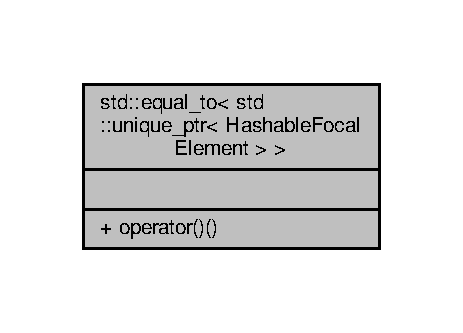
\includegraphics[width=222pt]{classstd_1_1equal__to_3_01std_1_1unique__ptr_3_01HashableFocalElement_01_4_01_4__coll__graph}
\end{center}
\end{figure}
\subsection*{Public Member Functions}
\begin{DoxyCompactItemize}
\item 
bool \hyperlink{classstd_1_1equal__to_3_01std_1_1unique__ptr_3_01HashableFocalElement_01_4_01_4_af20c9282247edd90edb92e620fadc5f4}{operator()} (const std\+::unique\+\_\+ptr$<$ \hyperlink{classHashableFocalElement}{Hashable\+Focal\+Element} $>$ \&h1, const std\+::unique\+\_\+ptr$<$ \hyperlink{classHashableFocalElement}{Hashable\+Focal\+Element} $>$ \&h2) const 
\end{DoxyCompactItemize}


\subsection{Member Function Documentation}
\hypertarget{classstd_1_1equal__to_3_01std_1_1unique__ptr_3_01HashableFocalElement_01_4_01_4_af20c9282247edd90edb92e620fadc5f4}{}\index{std\+::equal\+\_\+to$<$ std\+::unique\+\_\+ptr$<$ Hashable\+Focal\+Element $>$ $>$@{std\+::equal\+\_\+to$<$ std\+::unique\+\_\+ptr$<$ Hashable\+Focal\+Element $>$ $>$}!operator()@{operator()}}
\index{operator()@{operator()}!std\+::equal\+\_\+to$<$ std\+::unique\+\_\+ptr$<$ Hashable\+Focal\+Element $>$ $>$@{std\+::equal\+\_\+to$<$ std\+::unique\+\_\+ptr$<$ Hashable\+Focal\+Element $>$ $>$}}
\subsubsection[{operator()}]{\setlength{\rightskip}{0pt plus 5cm}bool std\+::equal\+\_\+to$<$ std\+::unique\+\_\+ptr$<$ {\bf Hashable\+Focal\+Element} $>$ $>$\+::operator() (
\begin{DoxyParamCaption}
\item[{const std\+::unique\+\_\+ptr$<$ {\bf Hashable\+Focal\+Element} $>$ \&}]{h1, }
\item[{const std\+::unique\+\_\+ptr$<$ {\bf Hashable\+Focal\+Element} $>$ \&}]{h2}
\end{DoxyParamCaption}
) const\hspace{0.3cm}{\ttfamily [inline]}}\label{classstd_1_1equal__to_3_01std_1_1unique__ptr_3_01HashableFocalElement_01_4_01_4_af20c9282247edd90edb92e620fadc5f4}


The documentation for this class was generated from the following file\+:\begin{DoxyCompactItemize}
\item 
focal\+\_\+elements/\hyperlink{HashableFocalElement_8h}{Hashable\+Focal\+Element.\+h}\end{DoxyCompactItemize}

\hypertarget{classEvidence}{}\section{Evidence Class Reference}
\label{classEvidence}\index{Evidence@{Evidence}}


Main class encapsulating the logic for the management of a belief assignment.  




{\ttfamily \#include $<$Evidence.\+h$>$}



Collaboration diagram for Evidence\+:\nopagebreak
\begin{figure}[H]
\begin{center}
\leavevmode
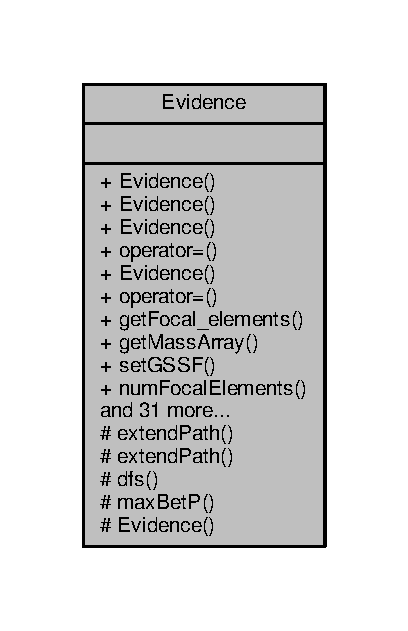
\includegraphics[width=196pt]{classEvidence__coll__graph}
\end{center}
\end{figure}
\subsection*{Public Member Functions}
\begin{DoxyCompactItemize}
\item 
\hyperlink{classEvidence_a85bcdfc070d0885b2c49c6930fe5a30f}{Evidence} (std\+::unique\+\_\+ptr$<$ \hyperlink{classFocalElement}{Focal\+Element} $>$ discernment\+\_\+frame, double \+\_\+ignorance=0)
\begin{DoxyCompactList}\small\item\em Constructor. \end{DoxyCompactList}\item 
\hyperlink{classEvidence_a0e7f11da2d686f8a33e3e59937b543d5}{Evidence} (std\+::unique\+\_\+ptr$<$ \hyperlink{classFocalElementContainerDispatcher}{Focal\+Element\+Container\+Dispatcher} $>$ dispatcher, std\+::unique\+\_\+ptr$<$ \hyperlink{classFocalElement}{Focal\+Element} $>$ discernment\+\_\+frame, double \+\_\+ignorance=0)
\begin{DoxyCompactList}\small\item\em Constructor. \end{DoxyCompactList}\item 
\hyperlink{classEvidence_a5e0b5cb75efbbcff102602ab07ed0ce5}{Evidence} (const \hyperlink{classEvidence}{Evidence} \&other)
\item 
\hyperlink{classEvidence}{Evidence} \& \hyperlink{classEvidence_a2e6f8b584bba250e859e4b8f16f286e2}{operator=} (const \hyperlink{classEvidence}{Evidence} \&other)
\item 
\hyperlink{classEvidence_a749172343fd62d98eb6c42636b5b61a4}{Evidence} (\hyperlink{classEvidence}{Evidence} \&\&other)=default
\item 
\hyperlink{classEvidence}{Evidence} \& \hyperlink{classEvidence_a02106bb9e91afce2555be1cd830862de}{operator=} (\hyperlink{classEvidence}{Evidence} \&\&other)=default
\item 
const std\+::vector$<$ std\+::unique\+\_\+ptr$<$ \hyperlink{classFocalElement}{Focal\+Element} $>$ $>$ \& \hyperlink{classEvidence_ab2d805af2fafd03c9d148040eeb181b0}{get\+Focal\+\_\+elements} () const 
\begin{DoxyCompactList}\small\item\em Get the focal elements. \end{DoxyCompactList}\item 
const std\+::vector$<$ double $>$ \& \hyperlink{classEvidence_a5cbcf217bf5159feccedba5edbd250c1}{get\+Mass\+Array} () const 
\begin{DoxyCompactList}\small\item\em Get the mass values. \end{DoxyCompactList}\item 
void \hyperlink{classEvidence_a9ebbf23d054f6202a8de321c4845341c}{set\+G\+S\+SF} ()
\begin{DoxyCompactList}\small\item\em Set it to be a Generic Simple Support Function. \end{DoxyCompactList}\item 
size\+\_\+t \hyperlink{classEvidence_af58901dda7c77519e3638b95304c4878}{num\+Focal\+Elements} () const 
\begin{DoxyCompactList}\small\item\em Get the number of focal elements. \end{DoxyCompactList}\item 
double \hyperlink{classEvidence_a095c85333b9be60da5e1f359357c23b5}{get\+Mass} (size\+\_\+t i) const 
\begin{DoxyCompactList}\small\item\em Get the mass at the given position. \end{DoxyCompactList}\item 
void \hyperlink{classEvidence_ac12ebfac60dd08a07c3e852e66903520}{set\+Mass} (double mass, \hyperlink{CMakeCache_8txt_a79a3d8790b2588b09777910863574e09}{int} index)
\begin{DoxyCompactList}\small\item\em Set the mass value at the given position. \end{DoxyCompactList}\item 
void \hyperlink{classEvidence_a854a8035ac5f008e9173edcfcf40f071}{set\+Mass} (double mass, const \hyperlink{classFocalElement}{Focal\+Element} \&fe)
\begin{DoxyCompactList}\small\item\em Set the mass value of the given \hyperlink{classFocalElement}{Focal\+Element}. \end{DoxyCompactList}\item 
double \hyperlink{classEvidence_af0aa3b6588833e3d707ce2f413daf46f}{get\+Mass} (const \hyperlink{classFocalElement}{Focal\+Element} \&fe) const 
\begin{DoxyCompactList}\small\item\em Get the mass value of the given \hyperlink{classFocalElement}{Focal\+Element}. \end{DoxyCompactList}\item 
void \hyperlink{classEvidence_a852aee625445547abfb4bb9a2031c10e}{delete\+Focal\+Element} (\hyperlink{CMakeCache_8txt_a79a3d8790b2588b09777910863574e09}{int} index)
\begin{DoxyCompactList}\small\item\em Delete the \hyperlink{classFocalElement}{Focal\+Element} at the given position. \end{DoxyCompactList}\item 
void \hyperlink{classEvidence_a1ebefa9999ec36cfd2fb782e6895e54c}{delete\+Focal\+Element} (const \hyperlink{classFocalElement}{Focal\+Element} \&fe)
\begin{DoxyCompactList}\small\item\em Delete the given \hyperlink{classFocalElement}{Focal\+Element}. \end{DoxyCompactList}\item 
void \hyperlink{classEvidence_a074be49ba8c3477d6d740a34ae2118b7}{add\+Focal\+Element} (std\+::unique\+\_\+ptr$<$ \hyperlink{classFocalElement}{Focal\+Element} $>$ elem, double mass)
\begin{DoxyCompactList}\small\item\em Add a new \hyperlink{classFocalElement}{Focal\+Element}. \end{DoxyCompactList}\item 
double \hyperlink{classEvidence_a65c3dd84b46113f721968869ee289edc}{conflict} () const 
\begin{DoxyCompactList}\small\item\em Calculate the conflict (mass of the empty set). \end{DoxyCompactList}\item 
bool \hyperlink{classEvidence_a4962e5c32a38d9c489ecb6afb6191c27}{is\+Consonant} () const 
\begin{DoxyCompactList}\small\item\em Checks if the B\+BA is consonant. \end{DoxyCompactList}\item 
double \hyperlink{classEvidence_ae50432e738f7aea56fe5802f1ec43cb7}{plausibility} (const \hyperlink{classFocalElement}{Focal\+Element} \&elem) const 
\begin{DoxyCompactList}\small\item\em Calculate the $Pl(A)$ of the \hyperlink{classFocalElement}{Focal\+Element} A. \end{DoxyCompactList}\item 
double \hyperlink{classEvidence_ac0b30688e56b6414e1a7733f58bec0dc}{belief} (const \hyperlink{classFocalElement}{Focal\+Element} \&elem) const 
\begin{DoxyCompactList}\small\item\em Calculate the $Bel(A)$ of the \hyperlink{classFocalElement}{Focal\+Element} A. \end{DoxyCompactList}\item 
double \hyperlink{classEvidence_a0374141346cfc31e86c9dd19659fbb0c}{q\+\_\+} (const \hyperlink{classFocalElement}{Focal\+Element} \&elem) const 
\begin{DoxyCompactList}\small\item\em Calculate the $q(A)$ of the \hyperlink{classFocalElement}{Focal\+Element} A. \end{DoxyCompactList}\item 
double \hyperlink{classEvidence_ae5e4bfa5009105ed1f61349eaad4cf9a}{BetP} (const \hyperlink{classFocalElement}{Focal\+Element} \&w) const 
\begin{DoxyCompactList}\small\item\em Calculate the $BetP(A)$ of the \hyperlink{classFocalElement}{Focal\+Element} A. \end{DoxyCompactList}\item 
double \hyperlink{classEvidence_ae417c974c680ef23eade3016e89b45b1}{BetP} (size\+\_\+t i) const 
\begin{DoxyCompactList}\small\item\em Calculate the $BetP(A)$ of the ith \hyperlink{classFocalElement}{Focal\+Element} A. \end{DoxyCompactList}\item 
std\+::unique\+\_\+ptr$<$ \hyperlink{classFocalElement}{Focal\+Element} $>$ \hyperlink{classEvidence_a2f311e3b5f265b2f138d3b48e4a3eefc}{max\+Bet\+P\+\_\+with\+Singletons} (\hyperlink{CMakeCache_8txt_a79a3d8790b2588b09777910863574e09}{int} approx\+\_\+step\+\_\+size=1) const 
\begin{DoxyCompactList}\small\item\em Find the \hyperlink{classFocalElement}{Focal\+Element} with maximum BetP by inspecting all the singleton Focal\+Elements included in the set. \end{DoxyCompactList}\item 
std\+::unique\+\_\+ptr$<$ \hyperlink{classFocalElement}{Focal\+Element} $>$ \hyperlink{classEvidence_a811a53979eb5a0b366fb47257ee6b920}{max\+Bet\+P\+\_\+with\+Maximal\+Intersections} () const 
\begin{DoxyCompactList}\small\item\em Find the \hyperlink{classFocalElement}{Focal\+Element} with maximum BetP by inspecting all the maximal intersections of the current set. \end{DoxyCompactList}\item 
bool \hyperlink{classEvidence_aab94dd76c710a6d4be701117a4c52039}{is\+Valid\+B\+BA} () const 
\begin{DoxyCompactList}\small\item\em Check if the B\+BA is valid. \end{DoxyCompactList}\item 
\hyperlink{classEvidence}{Evidence} \hyperlink{classEvidence_a798d5730a20db8baa86ae18a4bd9e23b}{conjunctive\+\_\+rule} (const \hyperlink{classEvidence}{Evidence} \&other, bool normalize\+Dempster=true) const 
\begin{DoxyCompactList}\small\item\em Conjunctive combination rule on two sources. \end{DoxyCompactList}\item 
\hyperlink{classEvidence}{Evidence} \hyperlink{classEvidence_af3739ab4923660f2a4ab00d118595781}{disjunctive\+\_\+rule} (const \hyperlink{classEvidence}{Evidence} \&other) const 
\begin{DoxyCompactList}\small\item\em Disjunctive combination rule on two sources. \end{DoxyCompactList}\item 
\hyperlink{classEvidence}{Evidence} \hyperlink{classEvidence_a20466c8101a61f8a8a716eda3e6b2c4c}{vacuous\+\_\+extension} (std\+::unique\+\_\+ptr$<$ \hyperlink{classFocalElement}{Focal\+Element} $>$ discernment\+\_\+frame\+\_\+2, bool extend\+\_\+right=true) const 
\begin{DoxyCompactList}\small\item\em Perform vacuous extension of the current B\+BA from discernment frame $\Omega_{1}$ to $\Omega_{1} \times \Omega_{2}$. \end{DoxyCompactList}\item 
\hyperlink{classEvidence}{Evidence} \hyperlink{classEvidence_a042d324e0ed4d3e07c87f16b4a1095ca}{marginalization} (bool marginalize\+\_\+right=true) const 
\begin{DoxyCompactList}\small\item\em Perform marginalization of the current B\+BA from $\Omega_{1} \times \Omega_{2}$ to $\Omega_{1}$. \end{DoxyCompactList}\item 
\hyperlink{classEvidence}{Evidence} \hyperlink{classEvidence_a209cebbffe359e12ccdd7743350b3ec3}{vacuous\+\_\+extension\+\_\+and\+\_\+conjuction} (const \hyperlink{classEvidence}{Evidence} \&other) const 
\begin{DoxyCompactList}\small\item\em Perform jointly vacuous extension and conjunction of two sources defined on two independent discernment frames. \end{DoxyCompactList}\item 
\hyperlink{classEvidence}{Evidence} \hyperlink{classEvidence_a1ad5b5d0d7df6fee326ba30aa4b015c6}{conditioning} (const \hyperlink{classFocalElement}{Focal\+Element} \&C) const 
\begin{DoxyCompactList}\small\item\em Perform conditioning operation on the current B\+BA. \end{DoxyCompactList}\item 
void \hyperlink{classEvidence_afaa46e0ce034a05c4749c7021430d60a}{discount} (double alpha)
\begin{DoxyCompactList}\small\item\em Perform discounting operator on the masses values. \end{DoxyCompactList}\item 
void \hyperlink{classEvidence_aa6a44be2f65aa439e2bdcf9333659abb}{normalize} ()
\begin{DoxyCompactList}\small\item\em Normalize the current B\+BA so that the conflict is zero. \end{DoxyCompactList}\item 
double \hyperlink{classEvidence_a2d6b2109c1347c004d00c2ef6bd515d8}{get\+Ignorance} () const 
\begin{DoxyCompactList}\small\item\em Get the ignorance (mass of the discernment frame). \end{DoxyCompactList}\item 
void \hyperlink{classEvidence_a11377c6946b7727015936b35dcf86cc8}{set\+Ignorance} (double ignorance)
\begin{DoxyCompactList}\small\item\em Set the ignorance (mass of discernment frame). \end{DoxyCompactList}\item 
const std\+::unique\+\_\+ptr$<$ \hyperlink{classFocalElement}{Focal\+Element} $>$ \& \hyperlink{classEvidence_a875150a8830c15d0cf3391d73889214e}{get\+Discernment\+\_\+frame} () const 
\begin{DoxyCompactList}\small\item\em Get the discernment frame. \end{DoxyCompactList}\end{DoxyCompactItemize}
\subsection*{Protected Member Functions}
\begin{DoxyCompactItemize}
\item 
void \hyperlink{classEvidence_a3d0206e5bbb6e8e61ad766c43d6e9113}{extend\+Path} (unsigned long long \&path, size\+\_\+t pos) const 
\item 
void \hyperlink{classEvidence_ae732467027722ccd1a3bd690110e21a3}{extend\+Path} (boost\+::dynamic\+\_\+bitset$<$$>$ \&path, size\+\_\+t pos) const 
\item 
{\footnotesize template$<$typename T $>$ }\\void \hyperlink{classEvidence_aaf90200d5b72268052a4c3df429b1932}{dfs} (std\+::unordered\+\_\+map$<$ size\+\_\+t, std\+::vector$<$ size\+\_\+t $>$$>$ \&adj\+\_\+list, size\+\_\+t current\+\_\+pos, T path, std\+::unique\+\_\+ptr$<$ \hyperlink{classFocalElement}{Focal\+Element} $>$ current\+\_\+intersection, std\+::vector$<$ std\+::unique\+\_\+ptr$<$ \hyperlink{classFocalElement}{Focal\+Element} $>$$>$ \&output\+\_\+vec, std\+::vector$<$ T $>$ \&check, std\+::vector$<$ size\+\_\+t $>$ \&indices, std\+::vector$<$ \hyperlink{CMakeCache_8txt_a79a3d8790b2588b09777910863574e09}{int} $>$ \&parents, size\+\_\+t cur\+\_\+root) const 
\item 
std\+::unique\+\_\+ptr$<$ \hyperlink{classFocalElement}{Focal\+Element} $>$ \hyperlink{classEvidence_aa2580207b322e297cdd0c3af07ddcd21}{max\+BetP} (std\+::vector$<$ std\+::unique\+\_\+ptr$<$ \hyperlink{classFocalElement}{Focal\+Element} $>$$>$ \&elems, bool compute\+Inters) const 
\item 
\hyperlink{classEvidence_a8136cd1d58c59e4b6a5088e9ac581797}{Evidence} (std\+::unique\+\_\+ptr$<$ \hyperlink{classFocalElementContainerDispatcher}{Focal\+Element\+Container\+Dispatcher} $>$ dispatcher, std\+::unique\+\_\+ptr$<$ \hyperlink{classFocalElementContainer}{Focal\+Element\+Container} $>$ \&\&fecontainer, std\+::unique\+\_\+ptr$<$ \hyperlink{classFocalElement}{Focal\+Element} $>$ discernment\+\_\+frame, double \+\_\+ignorance=0)
\end{DoxyCompactItemize}


\subsection{Detailed Description}
Main class encapsulating the logic for the management of a belief assignment. 

\subsection{Constructor \& Destructor Documentation}
\index{Evidence@{Evidence}!Evidence@{Evidence}}
\index{Evidence@{Evidence}!Evidence@{Evidence}}
\subsubsection[{\texorpdfstring{Evidence(std\+::unique\+\_\+ptr$<$ Focal\+Element\+Container\+Dispatcher $>$ dispatcher, std\+::unique\+\_\+ptr$<$ Focal\+Element\+Container $>$ \&\&fecontainer, std\+::unique\+\_\+ptr$<$ Focal\+Element $>$ discernment\+\_\+frame, double \+\_\+ignorance=0)}{Evidence(std::unique_ptr< FocalElementContainerDispatcher > dispatcher, std::unique_ptr< FocalElementContainer > &&fecontainer, std::unique_ptr< FocalElement > discernment_frame, double _ignorance=0)}}]{\setlength{\rightskip}{0pt plus 5cm}Evidence\+::\+Evidence (
\begin{DoxyParamCaption}
\item[{std\+::unique\+\_\+ptr$<$ {\bf Focal\+Element\+Container\+Dispatcher} $>$}]{dispatcher, }
\item[{std\+::unique\+\_\+ptr$<$ {\bf Focal\+Element\+Container} $>$ \&\&}]{fecontainer, }
\item[{std\+::unique\+\_\+ptr$<$ {\bf Focal\+Element} $>$}]{discernment\+\_\+frame, }
\item[{double}]{\+\_\+ignorance = {\ttfamily 0}}
\end{DoxyParamCaption}
)\hspace{0.3cm}{\ttfamily [explicit]}, {\ttfamily [protected]}}\hypertarget{classEvidence_a8136cd1d58c59e4b6a5088e9ac581797}{}\label{classEvidence_a8136cd1d58c59e4b6a5088e9ac581797}
\index{Evidence@{Evidence}!Evidence@{Evidence}}
\index{Evidence@{Evidence}!Evidence@{Evidence}}
\subsubsection[{\texorpdfstring{Evidence(std\+::unique\+\_\+ptr$<$ Focal\+Element $>$ discernment\+\_\+frame, double \+\_\+ignorance=0)}{Evidence(std::unique_ptr< FocalElement > discernment_frame, double _ignorance=0)}}]{\setlength{\rightskip}{0pt plus 5cm}Evidence\+::\+Evidence (
\begin{DoxyParamCaption}
\item[{std\+::unique\+\_\+ptr$<$ {\bf Focal\+Element} $>$}]{discernment\+\_\+frame, }
\item[{double}]{\+\_\+ignorance = {\ttfamily 0}}
\end{DoxyParamCaption}
)\hspace{0.3cm}{\ttfamily [explicit]}}\hypertarget{classEvidence_a85bcdfc070d0885b2c49c6930fe5a30f}{}\label{classEvidence_a85bcdfc070d0885b2c49c6930fe5a30f}


Constructor. 


\begin{DoxyParams}{Parameters}
{\em discernment\+\_\+frame} & The discernment frame. \\
\hline
{\em \+\_\+ignorance} & The ignorance value. \\
\hline
\end{DoxyParams}
\index{Evidence@{Evidence}!Evidence@{Evidence}}
\index{Evidence@{Evidence}!Evidence@{Evidence}}
\subsubsection[{\texorpdfstring{Evidence(std\+::unique\+\_\+ptr$<$ Focal\+Element\+Container\+Dispatcher $>$ dispatcher, std\+::unique\+\_\+ptr$<$ Focal\+Element $>$ discernment\+\_\+frame, double \+\_\+ignorance=0)}{Evidence(std::unique_ptr< FocalElementContainerDispatcher > dispatcher, std::unique_ptr< FocalElement > discernment_frame, double _ignorance=0)}}]{\setlength{\rightskip}{0pt plus 5cm}Evidence\+::\+Evidence (
\begin{DoxyParamCaption}
\item[{std\+::unique\+\_\+ptr$<$ {\bf Focal\+Element\+Container\+Dispatcher} $>$}]{dispatcher, }
\item[{std\+::unique\+\_\+ptr$<$ {\bf Focal\+Element} $>$}]{discernment\+\_\+frame, }
\item[{double}]{\+\_\+ignorance = {\ttfamily 0}}
\end{DoxyParamCaption}
)\hspace{0.3cm}{\ttfamily [explicit]}}\hypertarget{classEvidence_a0e7f11da2d686f8a33e3e59937b543d5}{}\label{classEvidence_a0e7f11da2d686f8a33e3e59937b543d5}


Constructor. 


\begin{DoxyParams}{Parameters}
{\em dispatcher} & The container dispatcher. \\
\hline
{\em discernment\+\_\+frame} & The discernment frame. \\
\hline
{\em \+\_\+ignorance} & The ignorance value. \\
\hline
\end{DoxyParams}
\index{Evidence@{Evidence}!Evidence@{Evidence}}
\index{Evidence@{Evidence}!Evidence@{Evidence}}
\subsubsection[{\texorpdfstring{Evidence(const Evidence \&other)}{Evidence(const Evidence &other)}}]{\setlength{\rightskip}{0pt plus 5cm}Evidence\+::\+Evidence (
\begin{DoxyParamCaption}
\item[{const {\bf Evidence} \&}]{other}
\end{DoxyParamCaption}
)}\hypertarget{classEvidence_a5e0b5cb75efbbcff102602ab07ed0ce5}{}\label{classEvidence_a5e0b5cb75efbbcff102602ab07ed0ce5}
\index{Evidence@{Evidence}!Evidence@{Evidence}}
\index{Evidence@{Evidence}!Evidence@{Evidence}}
\subsubsection[{\texorpdfstring{Evidence(\+Evidence \&\&other)=default}{Evidence(Evidence &&other)=default}}]{\setlength{\rightskip}{0pt plus 5cm}Evidence\+::\+Evidence (
\begin{DoxyParamCaption}
\item[{{\bf Evidence} \&\&}]{other}
\end{DoxyParamCaption}
)\hspace{0.3cm}{\ttfamily [default]}}\hypertarget{classEvidence_a749172343fd62d98eb6c42636b5b61a4}{}\label{classEvidence_a749172343fd62d98eb6c42636b5b61a4}


\subsection{Member Function Documentation}
\index{Evidence@{Evidence}!add\+Focal\+Element@{add\+Focal\+Element}}
\index{add\+Focal\+Element@{add\+Focal\+Element}!Evidence@{Evidence}}
\subsubsection[{\texorpdfstring{add\+Focal\+Element(std\+::unique\+\_\+ptr$<$ Focal\+Element $>$ elem, double mass)}{addFocalElement(std::unique_ptr< FocalElement > elem, double mass)}}]{\setlength{\rightskip}{0pt plus 5cm}void Evidence\+::add\+Focal\+Element (
\begin{DoxyParamCaption}
\item[{std\+::unique\+\_\+ptr$<$ {\bf Focal\+Element} $>$}]{elem, }
\item[{double}]{mass}
\end{DoxyParamCaption}
)}\hypertarget{classEvidence_a074be49ba8c3477d6d740a34ae2118b7}{}\label{classEvidence_a074be49ba8c3477d6d740a34ae2118b7}


Add a new \hyperlink{classFocalElement}{Focal\+Element}. 


\begin{DoxyParams}{Parameters}
{\em elem} & The \hyperlink{classFocalElement}{Focal\+Element}. \\
\hline
{\em mass} & The related mass value. \\
\hline
\end{DoxyParams}
\index{Evidence@{Evidence}!belief@{belief}}
\index{belief@{belief}!Evidence@{Evidence}}
\subsubsection[{\texorpdfstring{belief(const Focal\+Element \&elem) const }{belief(const FocalElement &elem) const }}]{\setlength{\rightskip}{0pt plus 5cm}double Evidence\+::belief (
\begin{DoxyParamCaption}
\item[{const {\bf Focal\+Element} \&}]{elem}
\end{DoxyParamCaption}
) const}\hypertarget{classEvidence_ac0b30688e56b6414e1a7733f58bec0dc}{}\label{classEvidence_ac0b30688e56b6414e1a7733f58bec0dc}


Calculate the $Bel(A)$ of the \hyperlink{classFocalElement}{Focal\+Element} A. 


\begin{DoxyParams}{Parameters}
{\em elem} & The \hyperlink{classFocalElement}{Focal\+Element}. \\
\hline
\end{DoxyParams}
\begin{DoxyReturn}{Returns}
Belief of elem. 
\end{DoxyReturn}
\index{Evidence@{Evidence}!BetP@{BetP}}
\index{BetP@{BetP}!Evidence@{Evidence}}
\subsubsection[{\texorpdfstring{Bet\+P(const Focal\+Element \&w) const }{BetP(const FocalElement &w) const }}]{\setlength{\rightskip}{0pt plus 5cm}double Evidence\+::\+BetP (
\begin{DoxyParamCaption}
\item[{const {\bf Focal\+Element} \&}]{w}
\end{DoxyParamCaption}
) const}\hypertarget{classEvidence_ae5e4bfa5009105ed1f61349eaad4cf9a}{}\label{classEvidence_ae5e4bfa5009105ed1f61349eaad4cf9a}


Calculate the $BetP(A)$ of the \hyperlink{classFocalElement}{Focal\+Element} A. 


\begin{DoxyParams}{Parameters}
{\em elem} & The \hyperlink{classFocalElement}{Focal\+Element}. \\
\hline
\end{DoxyParams}
\begin{DoxyReturn}{Returns}
BetP of elem. 
\end{DoxyReturn}
\index{Evidence@{Evidence}!BetP@{BetP}}
\index{BetP@{BetP}!Evidence@{Evidence}}
\subsubsection[{\texorpdfstring{Bet\+P(size\+\_\+t i) const }{BetP(size_t i) const }}]{\setlength{\rightskip}{0pt plus 5cm}double Evidence\+::\+BetP (
\begin{DoxyParamCaption}
\item[{size\+\_\+t}]{i}
\end{DoxyParamCaption}
) const}\hypertarget{classEvidence_ae417c974c680ef23eade3016e89b45b1}{}\label{classEvidence_ae417c974c680ef23eade3016e89b45b1}


Calculate the $BetP(A)$ of the ith \hyperlink{classFocalElement}{Focal\+Element} A. 


\begin{DoxyParams}{Parameters}
{\em i} & Position of A. \\
\hline
\end{DoxyParams}
\begin{DoxyReturn}{Returns}
BetP of A. 
\end{DoxyReturn}
\index{Evidence@{Evidence}!conditioning@{conditioning}}
\index{conditioning@{conditioning}!Evidence@{Evidence}}
\subsubsection[{\texorpdfstring{conditioning(const Focal\+Element \&\+C) const }{conditioning(const FocalElement &C) const }}]{\setlength{\rightskip}{0pt plus 5cm}{\bf Evidence} Evidence\+::conditioning (
\begin{DoxyParamCaption}
\item[{const {\bf Focal\+Element} \&}]{C}
\end{DoxyParamCaption}
) const}\hypertarget{classEvidence_a1ad5b5d0d7df6fee326ba30aa4b015c6}{}\label{classEvidence_a1ad5b5d0d7df6fee326ba30aa4b015c6}


Perform conditioning operation on the current B\+BA. 


\begin{DoxyParams}{Parameters}
{\em C} & The condition \hyperlink{classFocalElement}{Focal\+Element}. \\
\hline
\end{DoxyParams}
\begin{DoxyReturn}{Returns}
The B\+BA result of conditioning. 
\end{DoxyReturn}
\index{Evidence@{Evidence}!conflict@{conflict}}
\index{conflict@{conflict}!Evidence@{Evidence}}
\subsubsection[{\texorpdfstring{conflict() const }{conflict() const }}]{\setlength{\rightskip}{0pt plus 5cm}double Evidence\+::conflict (
\begin{DoxyParamCaption}
{}
\end{DoxyParamCaption}
) const}\hypertarget{classEvidence_a65c3dd84b46113f721968869ee289edc}{}\label{classEvidence_a65c3dd84b46113f721968869ee289edc}


Calculate the conflict (mass of the empty set). 

\begin{DoxyReturn}{Returns}
Conflict value. 
\end{DoxyReturn}
\index{Evidence@{Evidence}!conjunctive\+\_\+rule@{conjunctive\+\_\+rule}}
\index{conjunctive\+\_\+rule@{conjunctive\+\_\+rule}!Evidence@{Evidence}}
\subsubsection[{\texorpdfstring{conjunctive\+\_\+rule(const Evidence \&other, bool normalize\+Dempster=true) const }{conjunctive_rule(const Evidence &other, bool normalizeDempster=true) const }}]{\setlength{\rightskip}{0pt plus 5cm}{\bf Evidence} Evidence\+::conjunctive\+\_\+rule (
\begin{DoxyParamCaption}
\item[{const {\bf Evidence} \&}]{other, }
\item[{bool}]{normalize\+Dempster = {\ttfamily true}}
\end{DoxyParamCaption}
) const}\hypertarget{classEvidence_a798d5730a20db8baa86ae18a4bd9e23b}{}\label{classEvidence_a798d5730a20db8baa86ae18a4bd9e23b}


Conjunctive combination rule on two sources. 


\begin{DoxyParams}{Parameters}
{\em other} & The other B\+BA to combine with. \\
\hline
{\em normalize\+Dempster} & True if the Dempster Rule has to be applied for normalization. \\
\hline
\end{DoxyParams}
\begin{DoxyReturn}{Returns}
The B\+BA result of the conjuctive combination. 
\end{DoxyReturn}
\index{Evidence@{Evidence}!delete\+Focal\+Element@{delete\+Focal\+Element}}
\index{delete\+Focal\+Element@{delete\+Focal\+Element}!Evidence@{Evidence}}
\subsubsection[{\texorpdfstring{delete\+Focal\+Element(int index)}{deleteFocalElement(int index)}}]{\setlength{\rightskip}{0pt plus 5cm}void Evidence\+::delete\+Focal\+Element (
\begin{DoxyParamCaption}
\item[{{\bf int}}]{index}
\end{DoxyParamCaption}
)}\hypertarget{classEvidence_a852aee625445547abfb4bb9a2031c10e}{}\label{classEvidence_a852aee625445547abfb4bb9a2031c10e}


Delete the \hyperlink{classFocalElement}{Focal\+Element} at the given position. 


\begin{DoxyParams}{Parameters}
{\em index} & The target position \\
\hline
\end{DoxyParams}
\index{Evidence@{Evidence}!delete\+Focal\+Element@{delete\+Focal\+Element}}
\index{delete\+Focal\+Element@{delete\+Focal\+Element}!Evidence@{Evidence}}
\subsubsection[{\texorpdfstring{delete\+Focal\+Element(const Focal\+Element \&fe)}{deleteFocalElement(const FocalElement &fe)}}]{\setlength{\rightskip}{0pt plus 5cm}void Evidence\+::delete\+Focal\+Element (
\begin{DoxyParamCaption}
\item[{const {\bf Focal\+Element} \&}]{fe}
\end{DoxyParamCaption}
)}\hypertarget{classEvidence_a1ebefa9999ec36cfd2fb782e6895e54c}{}\label{classEvidence_a1ebefa9999ec36cfd2fb782e6895e54c}


Delete the given \hyperlink{classFocalElement}{Focal\+Element}. 


\begin{DoxyParams}{Parameters}
{\em fe} & The target \hyperlink{classFocalElement}{Focal\+Element} \\
\hline
\end{DoxyParams}
\index{Evidence@{Evidence}!dfs@{dfs}}
\index{dfs@{dfs}!Evidence@{Evidence}}
\subsubsection[{\texorpdfstring{dfs(std\+::unordered\+\_\+map$<$ size\+\_\+t, std\+::vector$<$ size\+\_\+t $>$$>$ \&adj\+\_\+list, size\+\_\+t current\+\_\+pos, T path, std\+::unique\+\_\+ptr$<$ Focal\+Element $>$ current\+\_\+intersection, std\+::vector$<$ std\+::unique\+\_\+ptr$<$ Focal\+Element $>$$>$ \&output\+\_\+vec, std\+::vector$<$ T $>$ \&check, std\+::vector$<$ size\+\_\+t $>$ \&indices, std\+::vector$<$ int $>$ \&parents, size\+\_\+t cur\+\_\+root) const }{dfs(std::unordered_map< size_t, std::vector< size_t >> &adj_list, size_t current_pos, T path, std::unique_ptr< FocalElement > current_intersection, std::vector< std::unique_ptr< FocalElement >> &output_vec, std::vector< T > &check, std::vector< size_t > &indices, std::vector< int > &parents, size_t cur_root) const }}]{\setlength{\rightskip}{0pt plus 5cm}template$<$typename T $>$ void Evidence\+::dfs (
\begin{DoxyParamCaption}
\item[{std\+::unordered\+\_\+map$<$ size\+\_\+t, std\+::vector$<$ size\+\_\+t $>$$>$ \&}]{adj\+\_\+list, }
\item[{size\+\_\+t}]{current\+\_\+pos, }
\item[{T}]{path, }
\item[{std\+::unique\+\_\+ptr$<$ {\bf Focal\+Element} $>$}]{current\+\_\+intersection, }
\item[{std\+::vector$<$ std\+::unique\+\_\+ptr$<$ {\bf Focal\+Element} $>$$>$ \&}]{output\+\_\+vec, }
\item[{std\+::vector$<$ T $>$ \&}]{check, }
\item[{std\+::vector$<$ size\+\_\+t $>$ \&}]{indices, }
\item[{std\+::vector$<$ {\bf int} $>$ \&}]{parents, }
\item[{size\+\_\+t}]{cur\+\_\+root}
\end{DoxyParamCaption}
) const\hspace{0.3cm}{\ttfamily [protected]}}\hypertarget{classEvidence_aaf90200d5b72268052a4c3df429b1932}{}\label{classEvidence_aaf90200d5b72268052a4c3df429b1932}
\index{Evidence@{Evidence}!discount@{discount}}
\index{discount@{discount}!Evidence@{Evidence}}
\subsubsection[{\texorpdfstring{discount(double alpha)}{discount(double alpha)}}]{\setlength{\rightskip}{0pt plus 5cm}void Evidence\+::discount (
\begin{DoxyParamCaption}
\item[{double}]{alpha}
\end{DoxyParamCaption}
)}\hypertarget{classEvidence_afaa46e0ce034a05c4749c7021430d60a}{}\label{classEvidence_afaa46e0ce034a05c4749c7021430d60a}


Perform discounting operator on the masses values. 


\begin{DoxyParams}{Parameters}
{\em alpha} & The discounting factor. \\
\hline
\end{DoxyParams}
\index{Evidence@{Evidence}!disjunctive\+\_\+rule@{disjunctive\+\_\+rule}}
\index{disjunctive\+\_\+rule@{disjunctive\+\_\+rule}!Evidence@{Evidence}}
\subsubsection[{\texorpdfstring{disjunctive\+\_\+rule(const Evidence \&other) const }{disjunctive_rule(const Evidence &other) const }}]{\setlength{\rightskip}{0pt plus 5cm}{\bf Evidence} Evidence\+::disjunctive\+\_\+rule (
\begin{DoxyParamCaption}
\item[{const {\bf Evidence} \&}]{other}
\end{DoxyParamCaption}
) const}\hypertarget{classEvidence_af3739ab4923660f2a4ab00d118595781}{}\label{classEvidence_af3739ab4923660f2a4ab00d118595781}


Disjunctive combination rule on two sources. 


\begin{DoxyParams}{Parameters}
{\em other} & The other B\+BA to combine with. \\
\hline
\end{DoxyParams}
\begin{DoxyReturn}{Returns}
The B\+BA result of the disjunctive combination. 
\end{DoxyReturn}
\index{Evidence@{Evidence}!extend\+Path@{extend\+Path}}
\index{extend\+Path@{extend\+Path}!Evidence@{Evidence}}
\subsubsection[{\texorpdfstring{extend\+Path(unsigned long long \&path, size\+\_\+t pos) const }{extendPath(unsigned long long &path, size_t pos) const }}]{\setlength{\rightskip}{0pt plus 5cm}void Evidence\+::extend\+Path (
\begin{DoxyParamCaption}
\item[{unsigned long long \&}]{path, }
\item[{size\+\_\+t}]{pos}
\end{DoxyParamCaption}
) const\hspace{0.3cm}{\ttfamily [protected]}}\hypertarget{classEvidence_a3d0206e5bbb6e8e61ad766c43d6e9113}{}\label{classEvidence_a3d0206e5bbb6e8e61ad766c43d6e9113}
\index{Evidence@{Evidence}!extend\+Path@{extend\+Path}}
\index{extend\+Path@{extend\+Path}!Evidence@{Evidence}}
\subsubsection[{\texorpdfstring{extend\+Path(boost\+::dynamic\+\_\+bitset$<$$>$ \&path, size\+\_\+t pos) const }{extendPath(boost::dynamic_bitset<> &path, size_t pos) const }}]{\setlength{\rightskip}{0pt plus 5cm}void Evidence\+::extend\+Path (
\begin{DoxyParamCaption}
\item[{boost\+::dynamic\+\_\+bitset$<$$>$ \&}]{path, }
\item[{size\+\_\+t}]{pos}
\end{DoxyParamCaption}
) const\hspace{0.3cm}{\ttfamily [protected]}}\hypertarget{classEvidence_ae732467027722ccd1a3bd690110e21a3}{}\label{classEvidence_ae732467027722ccd1a3bd690110e21a3}
\index{Evidence@{Evidence}!get\+Discernment\+\_\+frame@{get\+Discernment\+\_\+frame}}
\index{get\+Discernment\+\_\+frame@{get\+Discernment\+\_\+frame}!Evidence@{Evidence}}
\subsubsection[{\texorpdfstring{get\+Discernment\+\_\+frame() const }{getDiscernment_frame() const }}]{\setlength{\rightskip}{0pt plus 5cm}const std\+::unique\+\_\+ptr$<$ {\bf Focal\+Element} $>$ \& Evidence\+::get\+Discernment\+\_\+frame (
\begin{DoxyParamCaption}
{}
\end{DoxyParamCaption}
) const}\hypertarget{classEvidence_a875150a8830c15d0cf3391d73889214e}{}\label{classEvidence_a875150a8830c15d0cf3391d73889214e}


Get the discernment frame. 

\begin{DoxyReturn}{Returns}
Discernment frame. 
\end{DoxyReturn}
\index{Evidence@{Evidence}!get\+Focal\+\_\+elements@{get\+Focal\+\_\+elements}}
\index{get\+Focal\+\_\+elements@{get\+Focal\+\_\+elements}!Evidence@{Evidence}}
\subsubsection[{\texorpdfstring{get\+Focal\+\_\+elements() const }{getFocal_elements() const }}]{\setlength{\rightskip}{0pt plus 5cm}const std\+::vector$<$ std\+::unique\+\_\+ptr$<$ {\bf Focal\+Element} $>$ $>$ \& Evidence\+::get\+Focal\+\_\+elements (
\begin{DoxyParamCaption}
{}
\end{DoxyParamCaption}
) const}\hypertarget{classEvidence_ab2d805af2fafd03c9d148040eeb181b0}{}\label{classEvidence_ab2d805af2fafd03c9d148040eeb181b0}


Get the focal elements. 

\begin{DoxyReturn}{Returns}
Array of \hyperlink{classFocalElement}{Focal\+Element} objects. 
\end{DoxyReturn}
\index{Evidence@{Evidence}!get\+Ignorance@{get\+Ignorance}}
\index{get\+Ignorance@{get\+Ignorance}!Evidence@{Evidence}}
\subsubsection[{\texorpdfstring{get\+Ignorance() const }{getIgnorance() const }}]{\setlength{\rightskip}{0pt plus 5cm}double Evidence\+::get\+Ignorance (
\begin{DoxyParamCaption}
{}
\end{DoxyParamCaption}
) const}\hypertarget{classEvidence_a2d6b2109c1347c004d00c2ef6bd515d8}{}\label{classEvidence_a2d6b2109c1347c004d00c2ef6bd515d8}


Get the ignorance (mass of the discernment frame). 

\begin{DoxyReturn}{Returns}
Ignorance value. 
\end{DoxyReturn}
\index{Evidence@{Evidence}!get\+Mass@{get\+Mass}}
\index{get\+Mass@{get\+Mass}!Evidence@{Evidence}}
\subsubsection[{\texorpdfstring{get\+Mass(size\+\_\+t i) const }{getMass(size_t i) const }}]{\setlength{\rightskip}{0pt plus 5cm}double Evidence\+::get\+Mass (
\begin{DoxyParamCaption}
\item[{size\+\_\+t}]{i}
\end{DoxyParamCaption}
) const}\hypertarget{classEvidence_a095c85333b9be60da5e1f359357c23b5}{}\label{classEvidence_a095c85333b9be60da5e1f359357c23b5}


Get the mass at the given position. 


\begin{DoxyParams}{Parameters}
{\em i} & position \\
\hline
\end{DoxyParams}
\begin{DoxyReturn}{Returns}
The related mass 
\end{DoxyReturn}
\index{Evidence@{Evidence}!get\+Mass@{get\+Mass}}
\index{get\+Mass@{get\+Mass}!Evidence@{Evidence}}
\subsubsection[{\texorpdfstring{get\+Mass(const Focal\+Element \&fe) const }{getMass(const FocalElement &fe) const }}]{\setlength{\rightskip}{0pt plus 5cm}double Evidence\+::get\+Mass (
\begin{DoxyParamCaption}
\item[{const {\bf Focal\+Element} \&}]{fe}
\end{DoxyParamCaption}
) const}\hypertarget{classEvidence_af0aa3b6588833e3d707ce2f413daf46f}{}\label{classEvidence_af0aa3b6588833e3d707ce2f413daf46f}


Get the mass value of the given \hyperlink{classFocalElement}{Focal\+Element}. 


\begin{DoxyParams}{Parameters}
{\em fe} & The target \hyperlink{classFocalElement}{Focal\+Element} \\
\hline
\end{DoxyParams}
\begin{DoxyReturn}{Returns}
The related mass value. 
\end{DoxyReturn}
\index{Evidence@{Evidence}!get\+Mass\+Array@{get\+Mass\+Array}}
\index{get\+Mass\+Array@{get\+Mass\+Array}!Evidence@{Evidence}}
\subsubsection[{\texorpdfstring{get\+Mass\+Array() const }{getMassArray() const }}]{\setlength{\rightskip}{0pt plus 5cm}const std\+::vector$<$ double $>$ \& Evidence\+::get\+Mass\+Array (
\begin{DoxyParamCaption}
{}
\end{DoxyParamCaption}
) const}\hypertarget{classEvidence_a5cbcf217bf5159feccedba5edbd250c1}{}\label{classEvidence_a5cbcf217bf5159feccedba5edbd250c1}


Get the mass values. 

\begin{DoxyReturn}{Returns}
Array of masses. 
\end{DoxyReturn}
\index{Evidence@{Evidence}!is\+Consonant@{is\+Consonant}}
\index{is\+Consonant@{is\+Consonant}!Evidence@{Evidence}}
\subsubsection[{\texorpdfstring{is\+Consonant() const }{isConsonant() const }}]{\setlength{\rightskip}{0pt plus 5cm}bool Evidence\+::is\+Consonant (
\begin{DoxyParamCaption}
{}
\end{DoxyParamCaption}
) const}\hypertarget{classEvidence_a4962e5c32a38d9c489ecb6afb6191c27}{}\label{classEvidence_a4962e5c32a38d9c489ecb6afb6191c27}


Checks if the B\+BA is consonant. 

\begin{DoxyReturn}{Returns}
true if the B\+BA is consonant. 
\end{DoxyReturn}
\index{Evidence@{Evidence}!is\+Valid\+B\+BA@{is\+Valid\+B\+BA}}
\index{is\+Valid\+B\+BA@{is\+Valid\+B\+BA}!Evidence@{Evidence}}
\subsubsection[{\texorpdfstring{is\+Valid\+B\+B\+A() const }{isValidBBA() const }}]{\setlength{\rightskip}{0pt plus 5cm}bool Evidence\+::is\+Valid\+B\+BA (
\begin{DoxyParamCaption}
{}
\end{DoxyParamCaption}
) const}\hypertarget{classEvidence_aab94dd76c710a6d4be701117a4c52039}{}\label{classEvidence_aab94dd76c710a6d4be701117a4c52039}


Check if the B\+BA is valid. 

All the masses must be $>$0 and the conflict must be $>$=0. \begin{DoxyReturn}{Returns}
True if the current B\+BA is valid. 
\end{DoxyReturn}
\index{Evidence@{Evidence}!marginalization@{marginalization}}
\index{marginalization@{marginalization}!Evidence@{Evidence}}
\subsubsection[{\texorpdfstring{marginalization(bool marginalize\+\_\+right=true) const }{marginalization(bool marginalize_right=true) const }}]{\setlength{\rightskip}{0pt plus 5cm}{\bf Evidence} Evidence\+::marginalization (
\begin{DoxyParamCaption}
\item[{bool}]{marginalize\+\_\+right = {\ttfamily true}}
\end{DoxyParamCaption}
) const}\hypertarget{classEvidence_a042d324e0ed4d3e07c87f16b4a1095ca}{}\label{classEvidence_a042d324e0ed4d3e07c87f16b4a1095ca}


Perform marginalization of the current B\+BA from $\Omega_{1} \times \Omega_{2}$ to $\Omega_{1}$. 


\begin{DoxyParams}{Parameters}
{\em marginalize\+\_\+right} & If true marginalize to $\Omega_{1}$, otherwise to $\Omega_{2}$ \\
\hline
\end{DoxyParams}
\begin{DoxyReturn}{Returns}
The B\+BA result of marginalization 
\end{DoxyReturn}
\index{Evidence@{Evidence}!max\+BetP@{max\+BetP}}
\index{max\+BetP@{max\+BetP}!Evidence@{Evidence}}
\subsubsection[{\texorpdfstring{max\+Bet\+P(std\+::vector$<$ std\+::unique\+\_\+ptr$<$ Focal\+Element $>$$>$ \&elems, bool compute\+Inters) const }{maxBetP(std::vector< std::unique_ptr< FocalElement >> &elems, bool computeInters) const }}]{\setlength{\rightskip}{0pt plus 5cm}std\+::unique\+\_\+ptr$<$ {\bf Focal\+Element} $>$ Evidence\+::max\+BetP (
\begin{DoxyParamCaption}
\item[{std\+::vector$<$ std\+::unique\+\_\+ptr$<$ {\bf Focal\+Element} $>$$>$ \&}]{elems, }
\item[{bool}]{compute\+Inters}
\end{DoxyParamCaption}
) const\hspace{0.3cm}{\ttfamily [protected]}}\hypertarget{classEvidence_aa2580207b322e297cdd0c3af07ddcd21}{}\label{classEvidence_aa2580207b322e297cdd0c3af07ddcd21}
\index{Evidence@{Evidence}!max\+Bet\+P\+\_\+with\+Maximal\+Intersections@{max\+Bet\+P\+\_\+with\+Maximal\+Intersections}}
\index{max\+Bet\+P\+\_\+with\+Maximal\+Intersections@{max\+Bet\+P\+\_\+with\+Maximal\+Intersections}!Evidence@{Evidence}}
\subsubsection[{\texorpdfstring{max\+Bet\+P\+\_\+with\+Maximal\+Intersections() const }{maxBetP_withMaximalIntersections() const }}]{\setlength{\rightskip}{0pt plus 5cm}std\+::unique\+\_\+ptr$<$ {\bf Focal\+Element} $>$ Evidence\+::max\+Bet\+P\+\_\+with\+Maximal\+Intersections (
\begin{DoxyParamCaption}
{}
\end{DoxyParamCaption}
) const}\hypertarget{classEvidence_a811a53979eb5a0b366fb47257ee6b920}{}\label{classEvidence_a811a53979eb5a0b366fb47257ee6b920}


Find the \hyperlink{classFocalElement}{Focal\+Element} with maximum BetP by inspecting all the maximal intersections of the current set. 

Maximal intersections are all the \hyperlink{classFocalElement}{Focal\+Element} intersections which are not contained into others (implying a lower BetP). \begin{DoxyReturn}{Returns}
The Focal\+E\+Lemt with maximum BetP 
\end{DoxyReturn}
\index{Evidence@{Evidence}!max\+Bet\+P\+\_\+with\+Singletons@{max\+Bet\+P\+\_\+with\+Singletons}}
\index{max\+Bet\+P\+\_\+with\+Singletons@{max\+Bet\+P\+\_\+with\+Singletons}!Evidence@{Evidence}}
\subsubsection[{\texorpdfstring{max\+Bet\+P\+\_\+with\+Singletons(int approx\+\_\+step\+\_\+size=1) const }{maxBetP_withSingletons(int approx_step_size=1) const }}]{\setlength{\rightskip}{0pt plus 5cm}std\+::unique\+\_\+ptr$<$ {\bf Focal\+Element} $>$ Evidence\+::max\+Bet\+P\+\_\+with\+Singletons (
\begin{DoxyParamCaption}
\item[{{\bf int}}]{approx\+\_\+step\+\_\+size = {\ttfamily 1}}
\end{DoxyParamCaption}
) const}\hypertarget{classEvidence_a2f311e3b5f265b2f138d3b48e4a3eefc}{}\label{classEvidence_a2f311e3b5f265b2f138d3b48e4a3eefc}


Find the \hyperlink{classFocalElement}{Focal\+Element} with maximum BetP by inspecting all the singleton Focal\+Elements included in the set. 

If the approx\+\_\+step\+\_\+size is greater than 1, the singletons are uniformly sampled, and an approximate solution is computed (useful for performance). 
\begin{DoxyParams}{Parameters}
{\em approx\+\_\+step\+\_\+size} & Sampling step of the singleton set \\
\hline
\end{DoxyParams}
\begin{DoxyReturn}{Returns}
The Focal\+E\+Lemt with maximum BetP 
\end{DoxyReturn}
\index{Evidence@{Evidence}!normalize@{normalize}}
\index{normalize@{normalize}!Evidence@{Evidence}}
\subsubsection[{\texorpdfstring{normalize()}{normalize()}}]{\setlength{\rightskip}{0pt plus 5cm}void Evidence\+::normalize (
\begin{DoxyParamCaption}
{}
\end{DoxyParamCaption}
)}\hypertarget{classEvidence_aa6a44be2f65aa439e2bdcf9333659abb}{}\label{classEvidence_aa6a44be2f65aa439e2bdcf9333659abb}


Normalize the current B\+BA so that the conflict is zero. 

\index{Evidence@{Evidence}!num\+Focal\+Elements@{num\+Focal\+Elements}}
\index{num\+Focal\+Elements@{num\+Focal\+Elements}!Evidence@{Evidence}}
\subsubsection[{\texorpdfstring{num\+Focal\+Elements() const }{numFocalElements() const }}]{\setlength{\rightskip}{0pt plus 5cm}size\+\_\+t Evidence\+::num\+Focal\+Elements (
\begin{DoxyParamCaption}
{}
\end{DoxyParamCaption}
) const}\hypertarget{classEvidence_af58901dda7c77519e3638b95304c4878}{}\label{classEvidence_af58901dda7c77519e3638b95304c4878}


Get the number of focal elements. 

\begin{DoxyReturn}{Returns}
Size of the \hyperlink{classFocalElement}{Focal\+Element} array. 
\end{DoxyReturn}
\index{Evidence@{Evidence}!operator=@{operator=}}
\index{operator=@{operator=}!Evidence@{Evidence}}
\subsubsection[{\texorpdfstring{operator=(const Evidence \&other)}{operator=(const Evidence &other)}}]{\setlength{\rightskip}{0pt plus 5cm}{\bf Evidence} \& Evidence\+::operator= (
\begin{DoxyParamCaption}
\item[{const {\bf Evidence} \&}]{other}
\end{DoxyParamCaption}
)}\hypertarget{classEvidence_a2e6f8b584bba250e859e4b8f16f286e2}{}\label{classEvidence_a2e6f8b584bba250e859e4b8f16f286e2}
\index{Evidence@{Evidence}!operator=@{operator=}}
\index{operator=@{operator=}!Evidence@{Evidence}}
\subsubsection[{\texorpdfstring{operator=(\+Evidence \&\&other)=default}{operator=(Evidence &&other)=default}}]{\setlength{\rightskip}{0pt plus 5cm}{\bf Evidence}\& Evidence\+::operator= (
\begin{DoxyParamCaption}
\item[{{\bf Evidence} \&\&}]{other}
\end{DoxyParamCaption}
)\hspace{0.3cm}{\ttfamily [default]}}\hypertarget{classEvidence_a02106bb9e91afce2555be1cd830862de}{}\label{classEvidence_a02106bb9e91afce2555be1cd830862de}
\index{Evidence@{Evidence}!plausibility@{plausibility}}
\index{plausibility@{plausibility}!Evidence@{Evidence}}
\subsubsection[{\texorpdfstring{plausibility(const Focal\+Element \&elem) const }{plausibility(const FocalElement &elem) const }}]{\setlength{\rightskip}{0pt plus 5cm}double Evidence\+::plausibility (
\begin{DoxyParamCaption}
\item[{const {\bf Focal\+Element} \&}]{elem}
\end{DoxyParamCaption}
) const}\hypertarget{classEvidence_ae50432e738f7aea56fe5802f1ec43cb7}{}\label{classEvidence_ae50432e738f7aea56fe5802f1ec43cb7}


Calculate the $Pl(A)$ of the \hyperlink{classFocalElement}{Focal\+Element} A. 


\begin{DoxyParams}{Parameters}
{\em elem} & The \hyperlink{classFocalElement}{Focal\+Element}. \\
\hline
\end{DoxyParams}
\begin{DoxyReturn}{Returns}
Plausibility of elem. 
\end{DoxyReturn}
\index{Evidence@{Evidence}!q\+\_\+@{q\+\_\+}}
\index{q\+\_\+@{q\+\_\+}!Evidence@{Evidence}}
\subsubsection[{\texorpdfstring{q\+\_\+(const Focal\+Element \&elem) const }{q_(const FocalElement &elem) const }}]{\setlength{\rightskip}{0pt plus 5cm}double Evidence\+::q\+\_\+ (
\begin{DoxyParamCaption}
\item[{const {\bf Focal\+Element} \&}]{elem}
\end{DoxyParamCaption}
) const}\hypertarget{classEvidence_a0374141346cfc31e86c9dd19659fbb0c}{}\label{classEvidence_a0374141346cfc31e86c9dd19659fbb0c}


Calculate the $q(A)$ of the \hyperlink{classFocalElement}{Focal\+Element} A. 


\begin{DoxyParams}{Parameters}
{\em elem} & The \hyperlink{classFocalElement}{Focal\+Element}. \\
\hline
\end{DoxyParams}
\begin{DoxyReturn}{Returns}
q of elem. 
\end{DoxyReturn}
\index{Evidence@{Evidence}!set\+G\+S\+SF@{set\+G\+S\+SF}}
\index{set\+G\+S\+SF@{set\+G\+S\+SF}!Evidence@{Evidence}}
\subsubsection[{\texorpdfstring{set\+G\+S\+S\+F()}{setGSSF()}}]{\setlength{\rightskip}{0pt plus 5cm}void Evidence\+::set\+G\+S\+SF (
\begin{DoxyParamCaption}
{}
\end{DoxyParamCaption}
)}\hypertarget{classEvidence_a9ebbf23d054f6202a8de321c4845341c}{}\label{classEvidence_a9ebbf23d054f6202a8de321c4845341c}


Set it to be a Generic Simple Support Function. 

Negative mass values will be allowed. \index{Evidence@{Evidence}!set\+Ignorance@{set\+Ignorance}}
\index{set\+Ignorance@{set\+Ignorance}!Evidence@{Evidence}}
\subsubsection[{\texorpdfstring{set\+Ignorance(double ignorance)}{setIgnorance(double ignorance)}}]{\setlength{\rightskip}{0pt plus 5cm}void Evidence\+::set\+Ignorance (
\begin{DoxyParamCaption}
\item[{double}]{ignorance}
\end{DoxyParamCaption}
)}\hypertarget{classEvidence_a11377c6946b7727015936b35dcf86cc8}{}\label{classEvidence_a11377c6946b7727015936b35dcf86cc8}


Set the ignorance (mass of discernment frame). 


\begin{DoxyParams}{Parameters}
{\em ignorance} & The new ignorance value. \\
\hline
\end{DoxyParams}
\index{Evidence@{Evidence}!set\+Mass@{set\+Mass}}
\index{set\+Mass@{set\+Mass}!Evidence@{Evidence}}
\subsubsection[{\texorpdfstring{set\+Mass(double mass, int index)}{setMass(double mass, int index)}}]{\setlength{\rightskip}{0pt plus 5cm}void Evidence\+::set\+Mass (
\begin{DoxyParamCaption}
\item[{double}]{mass, }
\item[{{\bf int}}]{index}
\end{DoxyParamCaption}
)}\hypertarget{classEvidence_ac12ebfac60dd08a07c3e852e66903520}{}\label{classEvidence_ac12ebfac60dd08a07c3e852e66903520}


Set the mass value at the given position. 


\begin{DoxyParams}{Parameters}
{\em mass} & The new mass value \\
\hline
{\em index} & Position \\
\hline
\end{DoxyParams}
\index{Evidence@{Evidence}!set\+Mass@{set\+Mass}}
\index{set\+Mass@{set\+Mass}!Evidence@{Evidence}}
\subsubsection[{\texorpdfstring{set\+Mass(double mass, const Focal\+Element \&fe)}{setMass(double mass, const FocalElement &fe)}}]{\setlength{\rightskip}{0pt plus 5cm}void Evidence\+::set\+Mass (
\begin{DoxyParamCaption}
\item[{double}]{mass, }
\item[{const {\bf Focal\+Element} \&}]{fe}
\end{DoxyParamCaption}
)}\hypertarget{classEvidence_a854a8035ac5f008e9173edcfcf40f071}{}\label{classEvidence_a854a8035ac5f008e9173edcfcf40f071}


Set the mass value of the given \hyperlink{classFocalElement}{Focal\+Element}. 


\begin{DoxyParams}{Parameters}
{\em mass} & The new mass value \\
\hline
{\em fe} & The target \hyperlink{classFocalElement}{Focal\+Element} \\
\hline
\end{DoxyParams}
\index{Evidence@{Evidence}!vacuous\+\_\+extension@{vacuous\+\_\+extension}}
\index{vacuous\+\_\+extension@{vacuous\+\_\+extension}!Evidence@{Evidence}}
\subsubsection[{\texorpdfstring{vacuous\+\_\+extension(std\+::unique\+\_\+ptr$<$ Focal\+Element $>$ discernment\+\_\+frame\+\_\+2, bool extend\+\_\+right=true) const }{vacuous_extension(std::unique_ptr< FocalElement > discernment_frame_2, bool extend_right=true) const }}]{\setlength{\rightskip}{0pt plus 5cm}{\bf Evidence} Evidence\+::vacuous\+\_\+extension (
\begin{DoxyParamCaption}
\item[{std\+::unique\+\_\+ptr$<$ {\bf Focal\+Element} $>$}]{discernment\+\_\+frame\+\_\+2, }
\item[{bool}]{extend\+\_\+right = {\ttfamily true}}
\end{DoxyParamCaption}
) const}\hypertarget{classEvidence_a20466c8101a61f8a8a716eda3e6b2c4c}{}\label{classEvidence_a20466c8101a61f8a8a716eda3e6b2c4c}


Perform vacuous extension of the current B\+BA from discernment frame $\Omega_{1}$ to $\Omega_{1} \times \Omega_{2}$. 


\begin{DoxyParams}{Parameters}
{\em discernment\+\_\+frame\+\_\+2} & $\Omega_{2}$ \\
\hline
{\em extend\+\_\+right} & If true, extend to $\Omega_{1} \times \Omega_{2}$, otherwise to $\Omega_{2} \times \Omega_{1}$ \\
\hline
\end{DoxyParams}
\begin{DoxyReturn}{Returns}
The B\+BA result of vacuous extension. 
\end{DoxyReturn}
\index{Evidence@{Evidence}!vacuous\+\_\+extension\+\_\+and\+\_\+conjuction@{vacuous\+\_\+extension\+\_\+and\+\_\+conjuction}}
\index{vacuous\+\_\+extension\+\_\+and\+\_\+conjuction@{vacuous\+\_\+extension\+\_\+and\+\_\+conjuction}!Evidence@{Evidence}}
\subsubsection[{\texorpdfstring{vacuous\+\_\+extension\+\_\+and\+\_\+conjuction(const Evidence \&other) const }{vacuous_extension_and_conjuction(const Evidence &other) const }}]{\setlength{\rightskip}{0pt plus 5cm}{\bf Evidence} Evidence\+::vacuous\+\_\+extension\+\_\+and\+\_\+conjuction (
\begin{DoxyParamCaption}
\item[{const {\bf Evidence} \&}]{other}
\end{DoxyParamCaption}
) const}\hypertarget{classEvidence_a209cebbffe359e12ccdd7743350b3ec3}{}\label{classEvidence_a209cebbffe359e12ccdd7743350b3ec3}


Perform jointly vacuous extension and conjunction of two sources defined on two independent discernment frames. 


\begin{DoxyParams}{Parameters}
{\em other} & The other B\+BA \\
\hline
\end{DoxyParams}
\begin{DoxyReturn}{Returns}
The B\+BA result of vacuous extension and conjunction. 
\end{DoxyReturn}


The documentation for this class was generated from the following files\+:\begin{DoxyCompactItemize}
\item 
\hyperlink{Evidence_8h}{Evidence.\+h}\item 
\hyperlink{Evidence_8cpp}{Evidence.\+cpp}\end{DoxyCompactItemize}

\hypertarget{classFocalElement}{}\section{Focal\+Element Class Reference}
\label{classFocalElement}\index{Focal\+Element@{Focal\+Element}}


{\ttfamily \#include $<$Focal\+Element.\+h$>$}



Inheritance diagram for Focal\+Element\+:
\nopagebreak
\begin{figure}[H]
\begin{center}
\leavevmode
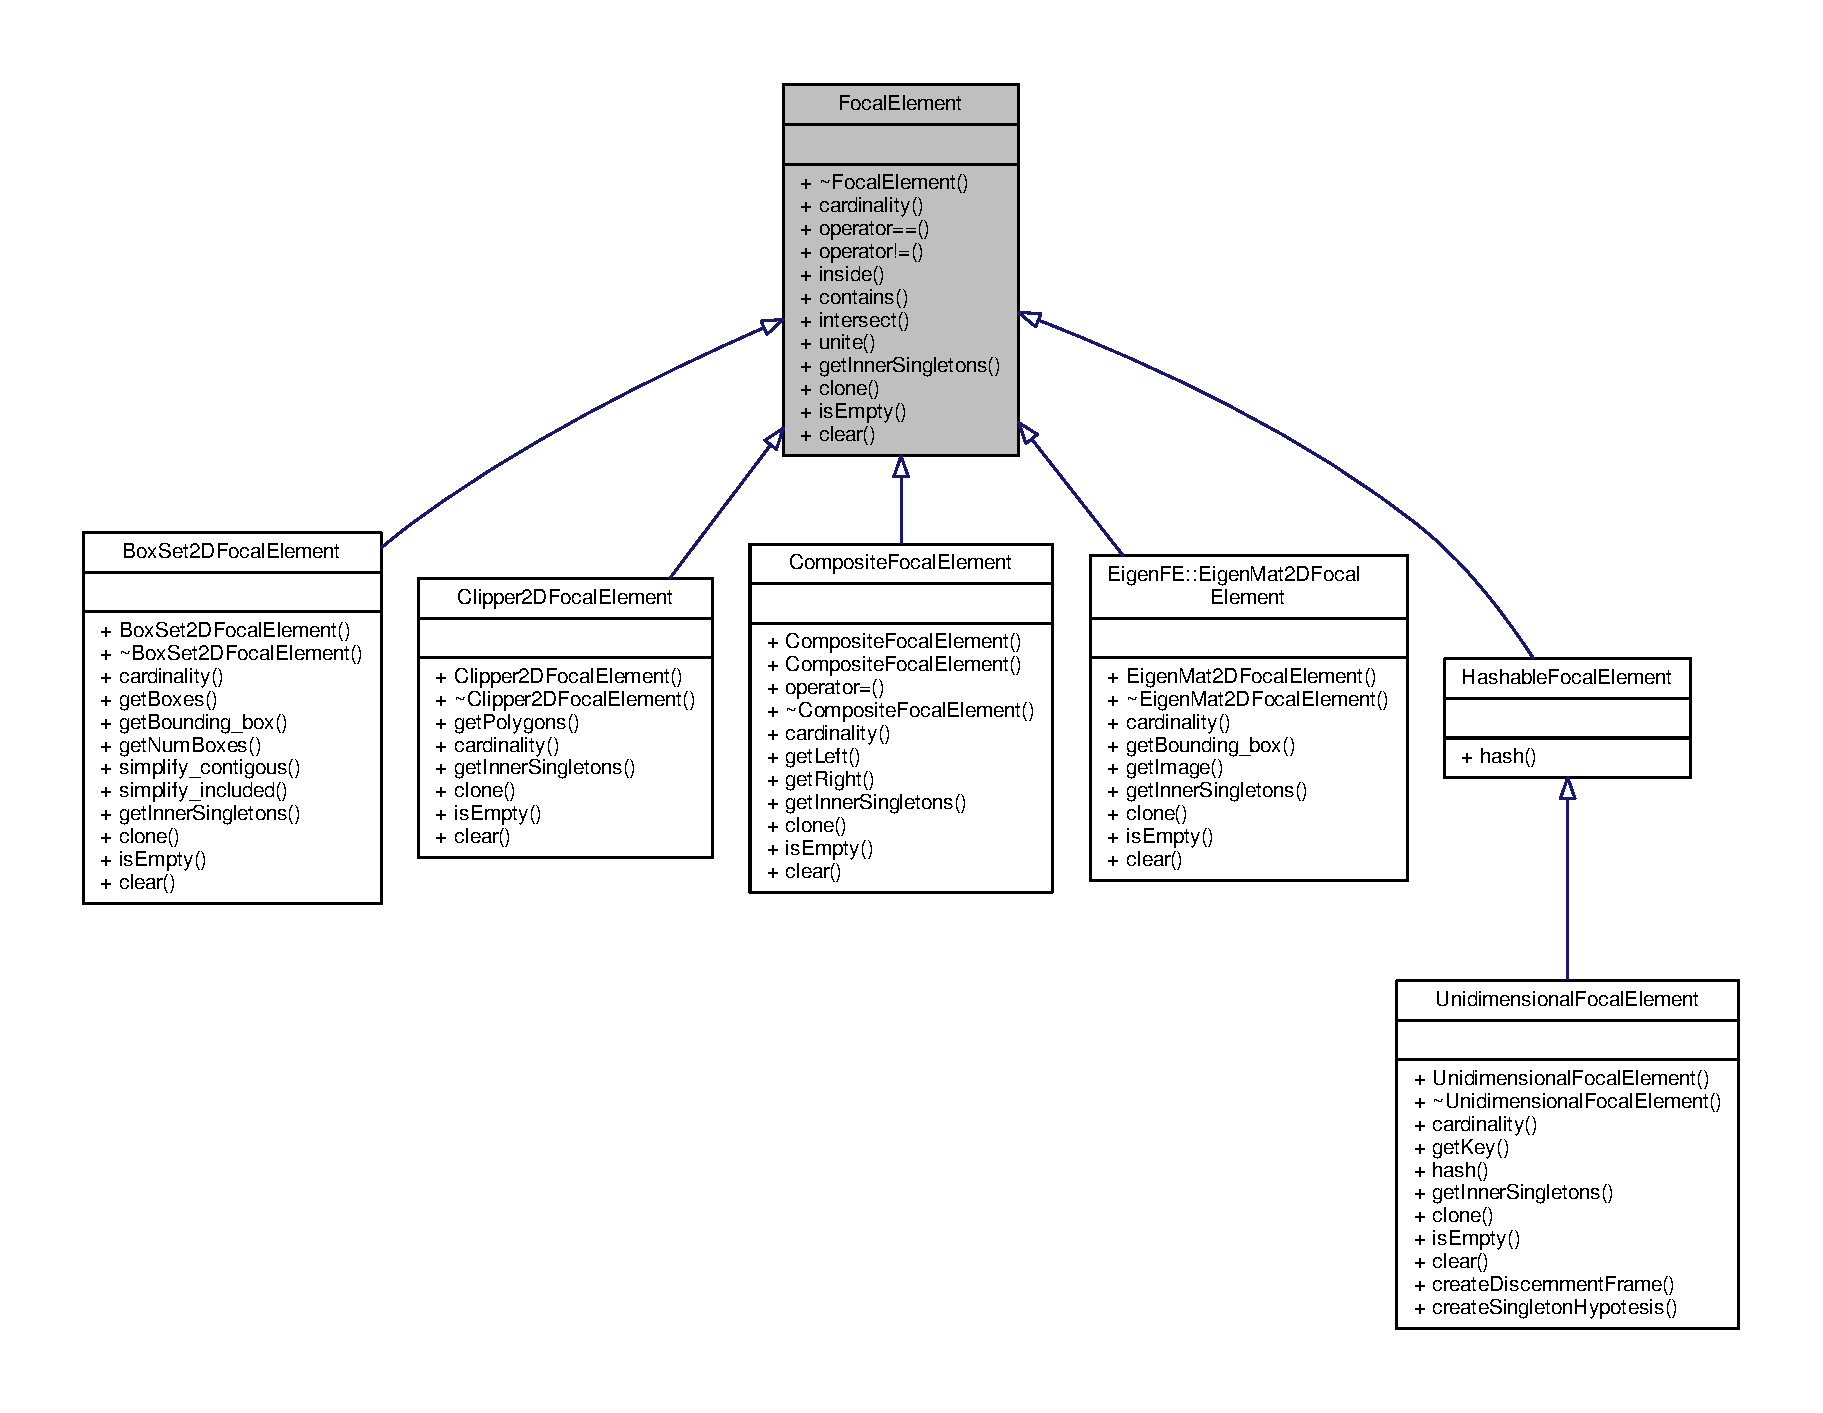
\includegraphics[width=350pt]{classFocalElement__inherit__graph}
\end{center}
\end{figure}


Collaboration diagram for Focal\+Element\+:\nopagebreak
\begin{figure}[H]
\begin{center}
\leavevmode
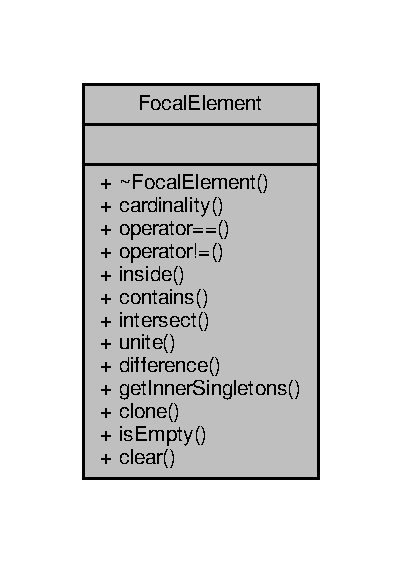
\includegraphics[width=193pt]{classFocalElement__coll__graph}
\end{center}
\end{figure}
\subsection*{Public Member Functions}
\begin{DoxyCompactItemize}
\item 
virtual \hyperlink{classFocalElement_a782f3f830a5cfa7242d519b8be3b4346}{$\sim$\+Focal\+Element} ()=default
\item 
virtual double \hyperlink{classFocalElement_a4ab1bbd0875e6e7ce2d7fe152e6a1639}{cardinality} () const =0
\item 
bool \hyperlink{classFocalElement_a431d66c098737bd6a64286a492b5ac65}{operator==} (const \hyperlink{classFocalElement}{Focal\+Element} \&rhs)
\item 
bool \hyperlink{classFocalElement_afde90486f09003215b51211c6546a9d3}{operator!=} (const \hyperlink{classFocalElement}{Focal\+Element} \&rhs)
\item 
bool \hyperlink{classFocalElement_aa1487ed49e7d203636edc8237322ed8b}{inside} (const \hyperlink{classFocalElement}{Focal\+Element} \&other) const 
\item 
bool \hyperlink{classFocalElement_acd424124e2ecff4b8c959d4874b89739}{contains} (const \hyperlink{classFocalElement}{Focal\+Element} \&other) const 
\item 
std\+::unique\+\_\+ptr$<$ \hyperlink{classFocalElement}{Focal\+Element} $>$ \hyperlink{classFocalElement_a2bb276626cceeca8f8ca46eafc923a04}{intersect} (const \hyperlink{classFocalElement}{Focal\+Element} \&other) const 
\item 
std\+::unique\+\_\+ptr$<$ \hyperlink{classFocalElement}{Focal\+Element} $>$ \hyperlink{classFocalElement_a533f16fbd5ae2b3d353d7c9a00bfb2c5}{unite} (const \hyperlink{classFocalElement}{Focal\+Element} \&other) const 
\item 
virtual std\+::vector$<$ std\+::unique\+\_\+ptr$<$ \hyperlink{classFocalElement}{Focal\+Element} $>$ $>$ \hyperlink{classFocalElement_ac615e960ea64a4bdc0f442135f6069e2}{get\+Inner\+Singletons} (int step\+\_\+size) const =0
\item 
virtual std\+::unique\+\_\+ptr$<$ \hyperlink{classFocalElement}{Focal\+Element} $>$ \hyperlink{classFocalElement_a21697fbbbcb144c18fa7b4ecae5e6145}{clone} () const =0
\item 
virtual bool \hyperlink{classFocalElement_aed131a65fdfc885019f9bf8f1d454508}{is\+Empty} () const =0
\item 
virtual void \hyperlink{classFocalElement_a635cb4afffa2dc69cf9fc9ff94a6d90f}{clear} ()=0
\end{DoxyCompactItemize}
\subsection*{Friends}
\begin{DoxyCompactItemize}
\item 
std\+::ostream \& \hyperlink{classFocalElement_a437885090fd5a00881653a501a4c70f1}{operator$<$$<$} (std\+::ostream \&os, const \hyperlink{classFocalElement}{Focal\+Element} \&element)
\end{DoxyCompactItemize}


\subsection{Constructor \& Destructor Documentation}
\hypertarget{classFocalElement_a782f3f830a5cfa7242d519b8be3b4346}{}\index{Focal\+Element@{Focal\+Element}!````~Focal\+Element@{$\sim$\+Focal\+Element}}
\index{````~Focal\+Element@{$\sim$\+Focal\+Element}!Focal\+Element@{Focal\+Element}}
\subsubsection[{$\sim$\+Focal\+Element}]{\setlength{\rightskip}{0pt plus 5cm}virtual Focal\+Element\+::$\sim$\+Focal\+Element (
\begin{DoxyParamCaption}
{}
\end{DoxyParamCaption}
)\hspace{0.3cm}{\ttfamily [virtual]}, {\ttfamily [default]}}\label{classFocalElement_a782f3f830a5cfa7242d519b8be3b4346}


\subsection{Member Function Documentation}
\hypertarget{classFocalElement_a4ab1bbd0875e6e7ce2d7fe152e6a1639}{}\index{Focal\+Element@{Focal\+Element}!cardinality@{cardinality}}
\index{cardinality@{cardinality}!Focal\+Element@{Focal\+Element}}
\subsubsection[{cardinality}]{\setlength{\rightskip}{0pt plus 5cm}virtual double Focal\+Element\+::cardinality (
\begin{DoxyParamCaption}
{}
\end{DoxyParamCaption}
) const\hspace{0.3cm}{\ttfamily [pure virtual]}}\label{classFocalElement_a4ab1bbd0875e6e7ce2d7fe152e6a1639}


Implemented in \hyperlink{classCompositeFocalElement_a18a671ee1759b5df42770384ace275fd}{Composite\+Focal\+Element}, \hyperlink{classBoxSet2DFocalElement_a65dd4942ec406f9048432654f81df964}{Box\+Set2\+D\+Focal\+Element}, \hyperlink{classEigenFE_1_1EigenMat2DFocalElement_ac19a1317772f2946bd8956cb084a3a1b}{Eigen\+F\+E\+::\+Eigen\+Mat2\+D\+Focal\+Element}, \hyperlink{classClipper2DFocalElement_a8eabcd9808b5b6bb7ec2f26eb89b5cd9}{Clipper2\+D\+Focal\+Element}, and \hyperlink{classUnidimensionalFocalElement_a22e013e2875cf07f23b3fe8ab2e2431f}{Unidimensional\+Focal\+Element}.

\hypertarget{classFocalElement_a635cb4afffa2dc69cf9fc9ff94a6d90f}{}\index{Focal\+Element@{Focal\+Element}!clear@{clear}}
\index{clear@{clear}!Focal\+Element@{Focal\+Element}}
\subsubsection[{clear}]{\setlength{\rightskip}{0pt plus 5cm}virtual void Focal\+Element\+::clear (
\begin{DoxyParamCaption}
{}
\end{DoxyParamCaption}
)\hspace{0.3cm}{\ttfamily [pure virtual]}}\label{classFocalElement_a635cb4afffa2dc69cf9fc9ff94a6d90f}


Implemented in \hyperlink{classBoxSet2DFocalElement_a9b09d64e1511def1a20898c7e3ac7390}{Box\+Set2\+D\+Focal\+Element}, \hyperlink{classCompositeFocalElement_a010c40507f9c45da7327f0418ea32b53}{Composite\+Focal\+Element}, \hyperlink{classUnidimensionalFocalElement_a1bd0c21e3e7e5a3ef78f4b47b98b6202}{Unidimensional\+Focal\+Element}, \hyperlink{classEigenFE_1_1EigenMat2DFocalElement_a32f67417ea35cb7d330d8ca27472c863}{Eigen\+F\+E\+::\+Eigen\+Mat2\+D\+Focal\+Element}, and \hyperlink{classClipper2DFocalElement_aa1110dabb3e01c681826374d1a485670}{Clipper2\+D\+Focal\+Element}.

\hypertarget{classFocalElement_a21697fbbbcb144c18fa7b4ecae5e6145}{}\index{Focal\+Element@{Focal\+Element}!clone@{clone}}
\index{clone@{clone}!Focal\+Element@{Focal\+Element}}
\subsubsection[{clone}]{\setlength{\rightskip}{0pt plus 5cm}virtual std\+::unique\+\_\+ptr$<${\bf Focal\+Element}$>$ Focal\+Element\+::clone (
\begin{DoxyParamCaption}
{}
\end{DoxyParamCaption}
) const\hspace{0.3cm}{\ttfamily [pure virtual]}}\label{classFocalElement_a21697fbbbcb144c18fa7b4ecae5e6145}


Implemented in \hyperlink{classBoxSet2DFocalElement_a0e325a4cad33db05c423f46eb1f346c9}{Box\+Set2\+D\+Focal\+Element}, \hyperlink{classCompositeFocalElement_a3ae99f9c094419664e443d650560baf4}{Composite\+Focal\+Element}, \hyperlink{classEigenFE_1_1EigenMat2DFocalElement_a7b11a9c1a340338ddc0502c04c3ebb50}{Eigen\+F\+E\+::\+Eigen\+Mat2\+D\+Focal\+Element}, \hyperlink{classUnidimensionalFocalElement_aa06e27bc6c262783704883477d630d60}{Unidimensional\+Focal\+Element}, and \hyperlink{classClipper2DFocalElement_a43aa82869ed3bf22682907ec9c475930}{Clipper2\+D\+Focal\+Element}.

\hypertarget{classFocalElement_acd424124e2ecff4b8c959d4874b89739}{}\index{Focal\+Element@{Focal\+Element}!contains@{contains}}
\index{contains@{contains}!Focal\+Element@{Focal\+Element}}
\subsubsection[{contains}]{\setlength{\rightskip}{0pt plus 5cm}bool Focal\+Element\+::contains (
\begin{DoxyParamCaption}
\item[{const {\bf Focal\+Element} \&}]{other}
\end{DoxyParamCaption}
) const\hspace{0.3cm}{\ttfamily [inline]}}\label{classFocalElement_acd424124e2ecff4b8c959d4874b89739}
\hypertarget{classFocalElement_ac615e960ea64a4bdc0f442135f6069e2}{}\index{Focal\+Element@{Focal\+Element}!get\+Inner\+Singletons@{get\+Inner\+Singletons}}
\index{get\+Inner\+Singletons@{get\+Inner\+Singletons}!Focal\+Element@{Focal\+Element}}
\subsubsection[{get\+Inner\+Singletons}]{\setlength{\rightskip}{0pt plus 5cm}virtual std\+::vector$<$std\+::unique\+\_\+ptr$<${\bf Focal\+Element}$>$ $>$ Focal\+Element\+::get\+Inner\+Singletons (
\begin{DoxyParamCaption}
\item[{int}]{step\+\_\+size}
\end{DoxyParamCaption}
) const\hspace{0.3cm}{\ttfamily [pure virtual]}}\label{classFocalElement_ac615e960ea64a4bdc0f442135f6069e2}


Implemented in \hyperlink{classBoxSet2DFocalElement_afdd0db628fc45a5865c72d9f1fb3fcce}{Box\+Set2\+D\+Focal\+Element}, \hyperlink{classCompositeFocalElement_aae945111cdffaaa5dc3216e439ac6ad2}{Composite\+Focal\+Element}, \hyperlink{classEigenFE_1_1EigenMat2DFocalElement_a02348604649107935c95106b1fb18a06}{Eigen\+F\+E\+::\+Eigen\+Mat2\+D\+Focal\+Element}, \hyperlink{classUnidimensionalFocalElement_ad37dc12733140cfd631d451ebfefcaf7}{Unidimensional\+Focal\+Element}, and \hyperlink{classClipper2DFocalElement_a2455cb3cc5940ecee3e012bcdcc25f44}{Clipper2\+D\+Focal\+Element}.

\hypertarget{classFocalElement_aa1487ed49e7d203636edc8237322ed8b}{}\index{Focal\+Element@{Focal\+Element}!inside@{inside}}
\index{inside@{inside}!Focal\+Element@{Focal\+Element}}
\subsubsection[{inside}]{\setlength{\rightskip}{0pt plus 5cm}bool Focal\+Element\+::inside (
\begin{DoxyParamCaption}
\item[{const {\bf Focal\+Element} \&}]{other}
\end{DoxyParamCaption}
) const\hspace{0.3cm}{\ttfamily [inline]}}\label{classFocalElement_aa1487ed49e7d203636edc8237322ed8b}
\hypertarget{classFocalElement_a2bb276626cceeca8f8ca46eafc923a04}{}\index{Focal\+Element@{Focal\+Element}!intersect@{intersect}}
\index{intersect@{intersect}!Focal\+Element@{Focal\+Element}}
\subsubsection[{intersect}]{\setlength{\rightskip}{0pt plus 5cm}std\+::unique\+\_\+ptr$<${\bf Focal\+Element}$>$ Focal\+Element\+::intersect (
\begin{DoxyParamCaption}
\item[{const {\bf Focal\+Element} \&}]{other}
\end{DoxyParamCaption}
) const\hspace{0.3cm}{\ttfamily [inline]}}\label{classFocalElement_a2bb276626cceeca8f8ca46eafc923a04}
\hypertarget{classFocalElement_aed131a65fdfc885019f9bf8f1d454508}{}\index{Focal\+Element@{Focal\+Element}!is\+Empty@{is\+Empty}}
\index{is\+Empty@{is\+Empty}!Focal\+Element@{Focal\+Element}}
\subsubsection[{is\+Empty}]{\setlength{\rightskip}{0pt plus 5cm}virtual bool Focal\+Element\+::is\+Empty (
\begin{DoxyParamCaption}
{}
\end{DoxyParamCaption}
) const\hspace{0.3cm}{\ttfamily [pure virtual]}}\label{classFocalElement_aed131a65fdfc885019f9bf8f1d454508}


Implemented in \hyperlink{classBoxSet2DFocalElement_a7512305b698f37aa77f3acacd0626f77}{Box\+Set2\+D\+Focal\+Element}, \hyperlink{classCompositeFocalElement_a015e5fa735f796d4ac38aec2e332b49a}{Composite\+Focal\+Element}, \hyperlink{classUnidimensionalFocalElement_a836c8a041ffba3e3e2ff7e584469a650}{Unidimensional\+Focal\+Element}, \hyperlink{classEigenFE_1_1EigenMat2DFocalElement_af0b7bcf11590355059f49c59c51aea3f}{Eigen\+F\+E\+::\+Eigen\+Mat2\+D\+Focal\+Element}, and \hyperlink{classClipper2DFocalElement_ae79aa59bb6a1109d729a32240631d573}{Clipper2\+D\+Focal\+Element}.

\hypertarget{classFocalElement_afde90486f09003215b51211c6546a9d3}{}\index{Focal\+Element@{Focal\+Element}!operator"!=@{operator"!=}}
\index{operator"!=@{operator"!=}!Focal\+Element@{Focal\+Element}}
\subsubsection[{operator"!=}]{\setlength{\rightskip}{0pt plus 5cm}bool Focal\+Element\+::operator!= (
\begin{DoxyParamCaption}
\item[{const {\bf Focal\+Element} \&}]{rhs}
\end{DoxyParamCaption}
)\hspace{0.3cm}{\ttfamily [inline]}}\label{classFocalElement_afde90486f09003215b51211c6546a9d3}
\hypertarget{classFocalElement_a431d66c098737bd6a64286a492b5ac65}{}\index{Focal\+Element@{Focal\+Element}!operator==@{operator==}}
\index{operator==@{operator==}!Focal\+Element@{Focal\+Element}}
\subsubsection[{operator==}]{\setlength{\rightskip}{0pt plus 5cm}bool Focal\+Element\+::operator== (
\begin{DoxyParamCaption}
\item[{const {\bf Focal\+Element} \&}]{rhs}
\end{DoxyParamCaption}
)\hspace{0.3cm}{\ttfamily [inline]}}\label{classFocalElement_a431d66c098737bd6a64286a492b5ac65}
\hypertarget{classFocalElement_a533f16fbd5ae2b3d353d7c9a00bfb2c5}{}\index{Focal\+Element@{Focal\+Element}!unite@{unite}}
\index{unite@{unite}!Focal\+Element@{Focal\+Element}}
\subsubsection[{unite}]{\setlength{\rightskip}{0pt plus 5cm}std\+::unique\+\_\+ptr$<${\bf Focal\+Element}$>$ Focal\+Element\+::unite (
\begin{DoxyParamCaption}
\item[{const {\bf Focal\+Element} \&}]{other}
\end{DoxyParamCaption}
) const\hspace{0.3cm}{\ttfamily [inline]}}\label{classFocalElement_a533f16fbd5ae2b3d353d7c9a00bfb2c5}


\subsection{Friends And Related Function Documentation}
\hypertarget{classFocalElement_a437885090fd5a00881653a501a4c70f1}{}\index{Focal\+Element@{Focal\+Element}!operator$<$$<$@{operator$<$$<$}}
\index{operator$<$$<$@{operator$<$$<$}!Focal\+Element@{Focal\+Element}}
\subsubsection[{operator$<$$<$}]{\setlength{\rightskip}{0pt plus 5cm}std\+::ostream\& operator$<$$<$ (
\begin{DoxyParamCaption}
\item[{std\+::ostream \&}]{os, }
\item[{const {\bf Focal\+Element} \&}]{element}
\end{DoxyParamCaption}
)\hspace{0.3cm}{\ttfamily [friend]}}\label{classFocalElement_a437885090fd5a00881653a501a4c70f1}


The documentation for this class was generated from the following file\+:\begin{DoxyCompactItemize}
\item 
focal\+\_\+elements/\hyperlink{FocalElement_8h}{Focal\+Element.\+h}\end{DoxyCompactItemize}

\hypertarget{classFocalElementContainer}{}\section{Focal\+Element\+Container Class Reference}
\label{classFocalElementContainer}\index{Focal\+Element\+Container@{Focal\+Element\+Container}}


Container of \hyperlink{classFocalElement}{Focal\+Element} objects.  




{\ttfamily \#include $<$Focal\+Element\+Container.\+h$>$}



Inheritance diagram for Focal\+Element\+Container\+:
\nopagebreak
\begin{figure}[H]
\begin{center}
\leavevmode
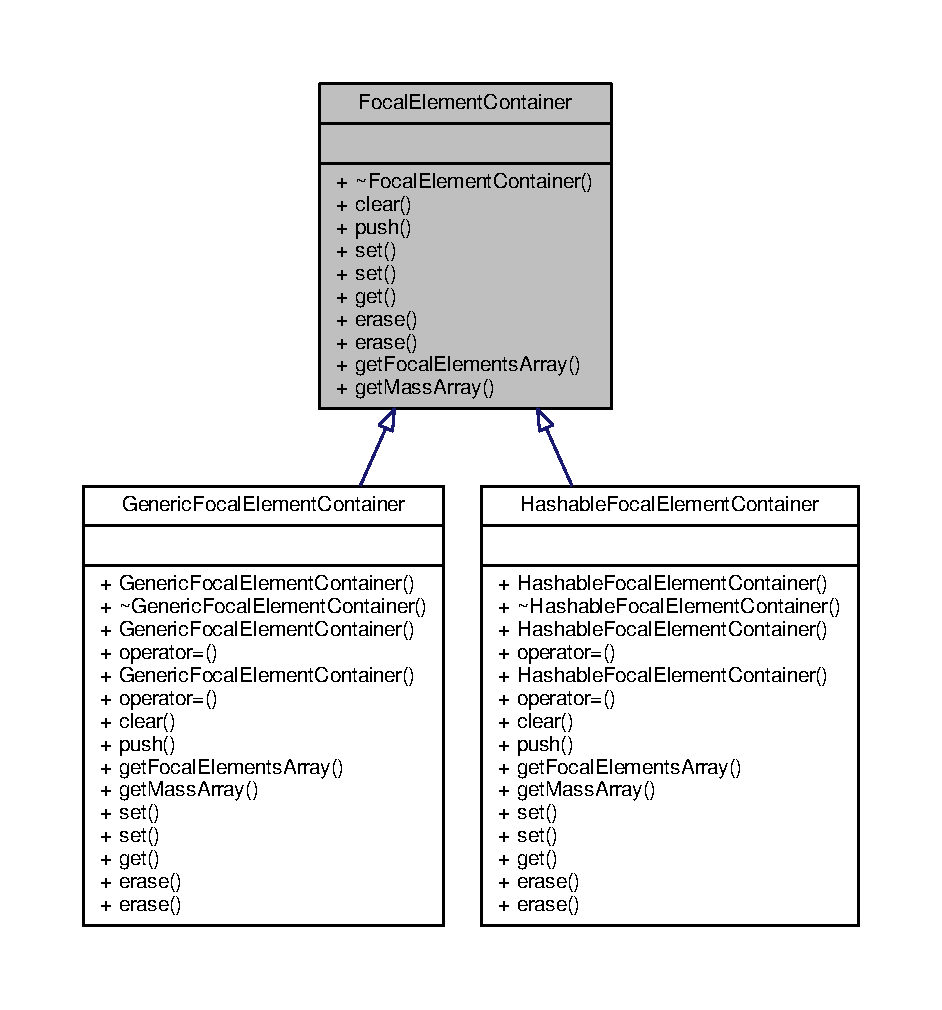
\includegraphics[width=350pt]{classFocalElementContainer__inherit__graph}
\end{center}
\end{figure}


Collaboration diagram for Focal\+Element\+Container\+:\nopagebreak
\begin{figure}[H]
\begin{center}
\leavevmode
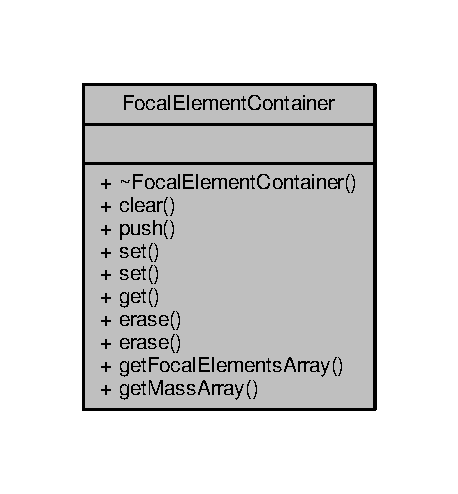
\includegraphics[width=220pt]{classFocalElementContainer__coll__graph}
\end{center}
\end{figure}
\subsection*{Public Member Functions}
\begin{DoxyCompactItemize}
\item 
virtual \hyperlink{classFocalElementContainer_a939ab96df66f872bf1600e9536c15aaf}{$\sim$\+Focal\+Element\+Container} ()=default
\item 
virtual void \hyperlink{classFocalElementContainer_a79977845eba147c3d29d8c500dbe593c}{clear} ()=0
\begin{DoxyCompactList}\small\item\em Clear the container. \end{DoxyCompactList}\item 
virtual void \hyperlink{classFocalElementContainer_a951895e83f8ef4ba79fa1c45d2d3c1ac}{push} (std\+::unique\+\_\+ptr$<$ \hyperlink{classFocalElement}{Focal\+Element} $>$ elem, double mass)=0
\begin{DoxyCompactList}\small\item\em Add a new \hyperlink{classFocalElement}{Focal\+Element} to the container. \end{DoxyCompactList}\item 
virtual void \hyperlink{classFocalElementContainer_a37edfcf750dfc72a7f3a92a2ab6bd62e}{set} (int index, double mass)=0
\begin{DoxyCompactList}\small\item\em Set the mass value at a given position. \end{DoxyCompactList}\item 
virtual void \hyperlink{classFocalElementContainer_a444a088fc937650226f2ecdd1db59510}{set} (const \hyperlink{classFocalElement}{Focal\+Element} \&fe, double mass)=0
\begin{DoxyCompactList}\small\item\em Set the mass value of the given \hyperlink{classFocalElement}{Focal\+Element}. \end{DoxyCompactList}\item 
virtual double \hyperlink{classFocalElementContainer_a5ffaa25475069d4868cec5a73ccf314f}{get} (const \hyperlink{classFocalElement}{Focal\+Element} \&fe)=0
\begin{DoxyCompactList}\small\item\em Get the mass value of the given \hyperlink{classFocalElement}{Focal\+Element}. \end{DoxyCompactList}\item 
virtual void \hyperlink{classFocalElementContainer_aaf91ad85eeb5b218171a142d7c3e1116}{erase} (int index)=0
\begin{DoxyCompactList}\small\item\em Erase the \hyperlink{classFocalElement}{Focal\+Element} at the given position. \end{DoxyCompactList}\item 
virtual void \hyperlink{classFocalElementContainer_af20780adab46a8d4e5b42c8b1934ea86}{erase} (const \hyperlink{classFocalElement}{Focal\+Element} \&fe)=0
\begin{DoxyCompactList}\small\item\em Erase the given \hyperlink{classFocalElement}{Focal\+Element}. \end{DoxyCompactList}\item 
virtual const std\+::vector$<$ std\+::unique\+\_\+ptr$<$ \hyperlink{classFocalElement}{Focal\+Element} $>$ $>$ \& \hyperlink{classFocalElementContainer_aa06ed4c0c21777cdc5256b576dc5e718}{get\+Focal\+Elements\+Array} ()=0
\begin{DoxyCompactList}\small\item\em Get the array of \hyperlink{classFocalElement}{Focal\+Element} object. \end{DoxyCompactList}\item 
virtual const std\+::vector$<$ double $>$ \& \hyperlink{classFocalElementContainer_a9197229964bfdf8765f81bf7b85c669d}{get\+Mass\+Array} ()=0
\begin{DoxyCompactList}\small\item\em Ge the array of masses. \end{DoxyCompactList}\end{DoxyCompactItemize}


\subsection{Detailed Description}
Container of \hyperlink{classFocalElement}{Focal\+Element} objects. 

\subsection{Constructor \& Destructor Documentation}
\hypertarget{classFocalElementContainer_a939ab96df66f872bf1600e9536c15aaf}{}\index{Focal\+Element\+Container@{Focal\+Element\+Container}!````~Focal\+Element\+Container@{$\sim$\+Focal\+Element\+Container}}
\index{````~Focal\+Element\+Container@{$\sim$\+Focal\+Element\+Container}!Focal\+Element\+Container@{Focal\+Element\+Container}}
\subsubsection[{$\sim$\+Focal\+Element\+Container}]{\setlength{\rightskip}{0pt plus 5cm}virtual Focal\+Element\+Container\+::$\sim$\+Focal\+Element\+Container (
\begin{DoxyParamCaption}
{}
\end{DoxyParamCaption}
)\hspace{0.3cm}{\ttfamily [virtual]}, {\ttfamily [default]}}\label{classFocalElementContainer_a939ab96df66f872bf1600e9536c15aaf}


\subsection{Member Function Documentation}
\hypertarget{classFocalElementContainer_a79977845eba147c3d29d8c500dbe593c}{}\index{Focal\+Element\+Container@{Focal\+Element\+Container}!clear@{clear}}
\index{clear@{clear}!Focal\+Element\+Container@{Focal\+Element\+Container}}
\subsubsection[{clear}]{\setlength{\rightskip}{0pt plus 5cm}virtual void Focal\+Element\+Container\+::clear (
\begin{DoxyParamCaption}
{}
\end{DoxyParamCaption}
)\hspace{0.3cm}{\ttfamily [pure virtual]}}\label{classFocalElementContainer_a79977845eba147c3d29d8c500dbe593c}


Clear the container. 



Implemented in \hyperlink{classHashableFocalElementContainer_a352c7bc7f6b705bd1a5d5e5b9ec225fe}{Hashable\+Focal\+Element\+Container}, and \hyperlink{classGenericFocalElementContainer_aa20631dceaa742116e6ad6ddf7a38555}{Generic\+Focal\+Element\+Container}.

\hypertarget{classFocalElementContainer_aaf91ad85eeb5b218171a142d7c3e1116}{}\index{Focal\+Element\+Container@{Focal\+Element\+Container}!erase@{erase}}
\index{erase@{erase}!Focal\+Element\+Container@{Focal\+Element\+Container}}
\subsubsection[{erase}]{\setlength{\rightskip}{0pt plus 5cm}virtual void Focal\+Element\+Container\+::erase (
\begin{DoxyParamCaption}
\item[{int}]{index}
\end{DoxyParamCaption}
)\hspace{0.3cm}{\ttfamily [pure virtual]}}\label{classFocalElementContainer_aaf91ad85eeb5b218171a142d7c3e1116}


Erase the \hyperlink{classFocalElement}{Focal\+Element} at the given position. 


\begin{DoxyParams}{Parameters}
{\em index} & The target position. \\
\hline
\end{DoxyParams}


Implemented in \hyperlink{classHashableFocalElementContainer_a06450d7d5174bdeecd2238570143e2b3}{Hashable\+Focal\+Element\+Container}, and \hyperlink{classGenericFocalElementContainer_a123f043d029c636824e4ca8153cd6aea}{Generic\+Focal\+Element\+Container}.

\hypertarget{classFocalElementContainer_af20780adab46a8d4e5b42c8b1934ea86}{}\index{Focal\+Element\+Container@{Focal\+Element\+Container}!erase@{erase}}
\index{erase@{erase}!Focal\+Element\+Container@{Focal\+Element\+Container}}
\subsubsection[{erase}]{\setlength{\rightskip}{0pt plus 5cm}virtual void Focal\+Element\+Container\+::erase (
\begin{DoxyParamCaption}
\item[{const {\bf Focal\+Element} \&}]{fe}
\end{DoxyParamCaption}
)\hspace{0.3cm}{\ttfamily [pure virtual]}}\label{classFocalElementContainer_af20780adab46a8d4e5b42c8b1934ea86}


Erase the given \hyperlink{classFocalElement}{Focal\+Element}. 


\begin{DoxyParams}{Parameters}
{\em fe} & The target \hyperlink{classFocalElement}{Focal\+Element}. \\
\hline
\end{DoxyParams}


Implemented in \hyperlink{classHashableFocalElementContainer_a8d072157c5715b764e3158427157a242}{Hashable\+Focal\+Element\+Container}, and \hyperlink{classGenericFocalElementContainer_a5bef7f21bc02455dd0cde6dbef69541a}{Generic\+Focal\+Element\+Container}.

\hypertarget{classFocalElementContainer_a5ffaa25475069d4868cec5a73ccf314f}{}\index{Focal\+Element\+Container@{Focal\+Element\+Container}!get@{get}}
\index{get@{get}!Focal\+Element\+Container@{Focal\+Element\+Container}}
\subsubsection[{get}]{\setlength{\rightskip}{0pt plus 5cm}virtual double Focal\+Element\+Container\+::get (
\begin{DoxyParamCaption}
\item[{const {\bf Focal\+Element} \&}]{fe}
\end{DoxyParamCaption}
)\hspace{0.3cm}{\ttfamily [pure virtual]}}\label{classFocalElementContainer_a5ffaa25475069d4868cec5a73ccf314f}


Get the mass value of the given \hyperlink{classFocalElement}{Focal\+Element}. 


\begin{DoxyParams}{Parameters}
{\em fe} & The target \hyperlink{classFocalElement}{Focal\+Element} \\
\hline
\end{DoxyParams}
\begin{DoxyReturn}{Returns}
The associated mass value 
\end{DoxyReturn}


Implemented in \hyperlink{classHashableFocalElementContainer_a0b384b37bee91526a932756a65727be0}{Hashable\+Focal\+Element\+Container}, and \hyperlink{classGenericFocalElementContainer_a3a9fd25120f480a33770e52d198ecc33}{Generic\+Focal\+Element\+Container}.

\hypertarget{classFocalElementContainer_aa06ed4c0c21777cdc5256b576dc5e718}{}\index{Focal\+Element\+Container@{Focal\+Element\+Container}!get\+Focal\+Elements\+Array@{get\+Focal\+Elements\+Array}}
\index{get\+Focal\+Elements\+Array@{get\+Focal\+Elements\+Array}!Focal\+Element\+Container@{Focal\+Element\+Container}}
\subsubsection[{get\+Focal\+Elements\+Array}]{\setlength{\rightskip}{0pt plus 5cm}virtual const std\+::vector$<$std\+::unique\+\_\+ptr$<${\bf Focal\+Element}$>$ $>$\& Focal\+Element\+Container\+::get\+Focal\+Elements\+Array (
\begin{DoxyParamCaption}
{}
\end{DoxyParamCaption}
)\hspace{0.3cm}{\ttfamily [pure virtual]}}\label{classFocalElementContainer_aa06ed4c0c21777cdc5256b576dc5e718}


Get the array of \hyperlink{classFocalElement}{Focal\+Element} object. 

\begin{DoxyReturn}{Returns}
Array of \hyperlink{classFocalElement}{Focal\+Element}. 
\end{DoxyReturn}


Implemented in \hyperlink{classHashableFocalElementContainer_a11ab286119f448d1a480dd4336875b9f}{Hashable\+Focal\+Element\+Container}, and \hyperlink{classGenericFocalElementContainer_a2db442b704235b974d96cd5670ab1630}{Generic\+Focal\+Element\+Container}.

\hypertarget{classFocalElementContainer_a9197229964bfdf8765f81bf7b85c669d}{}\index{Focal\+Element\+Container@{Focal\+Element\+Container}!get\+Mass\+Array@{get\+Mass\+Array}}
\index{get\+Mass\+Array@{get\+Mass\+Array}!Focal\+Element\+Container@{Focal\+Element\+Container}}
\subsubsection[{get\+Mass\+Array}]{\setlength{\rightskip}{0pt plus 5cm}virtual const std\+::vector$<$double$>$\& Focal\+Element\+Container\+::get\+Mass\+Array (
\begin{DoxyParamCaption}
{}
\end{DoxyParamCaption}
)\hspace{0.3cm}{\ttfamily [pure virtual]}}\label{classFocalElementContainer_a9197229964bfdf8765f81bf7b85c669d}


Ge the array of masses. 

\begin{DoxyReturn}{Returns}
Array of masses. 
\end{DoxyReturn}


Implemented in \hyperlink{classHashableFocalElementContainer_a8be85b980960704d31563d0ad64b8aad}{Hashable\+Focal\+Element\+Container}, and \hyperlink{classGenericFocalElementContainer_a0ae8e8ad18f3d8c09db25688f2da684b}{Generic\+Focal\+Element\+Container}.

\hypertarget{classFocalElementContainer_a951895e83f8ef4ba79fa1c45d2d3c1ac}{}\index{Focal\+Element\+Container@{Focal\+Element\+Container}!push@{push}}
\index{push@{push}!Focal\+Element\+Container@{Focal\+Element\+Container}}
\subsubsection[{push}]{\setlength{\rightskip}{0pt plus 5cm}virtual void Focal\+Element\+Container\+::push (
\begin{DoxyParamCaption}
\item[{std\+::unique\+\_\+ptr$<$ {\bf Focal\+Element} $>$}]{elem, }
\item[{double}]{mass}
\end{DoxyParamCaption}
)\hspace{0.3cm}{\ttfamily [pure virtual]}}\label{classFocalElementContainer_a951895e83f8ef4ba79fa1c45d2d3c1ac}


Add a new \hyperlink{classFocalElement}{Focal\+Element} to the container. 


\begin{DoxyParams}{Parameters}
{\em elem} & The \hyperlink{classFocalElement}{Focal\+Element} to be added. \\
\hline
{\em mass} & The mass value. \\
\hline
\end{DoxyParams}


Implemented in \hyperlink{classHashableFocalElementContainer_a896a7b5c2719e63b1ad8a53a6d33c6c7}{Hashable\+Focal\+Element\+Container}, and \hyperlink{classGenericFocalElementContainer_aefcc139561645f96f3ec877992005d2b}{Generic\+Focal\+Element\+Container}.

\hypertarget{classFocalElementContainer_a37edfcf750dfc72a7f3a92a2ab6bd62e}{}\index{Focal\+Element\+Container@{Focal\+Element\+Container}!set@{set}}
\index{set@{set}!Focal\+Element\+Container@{Focal\+Element\+Container}}
\subsubsection[{set}]{\setlength{\rightskip}{0pt plus 5cm}virtual void Focal\+Element\+Container\+::set (
\begin{DoxyParamCaption}
\item[{int}]{index, }
\item[{double}]{mass}
\end{DoxyParamCaption}
)\hspace{0.3cm}{\ttfamily [pure virtual]}}\label{classFocalElementContainer_a37edfcf750dfc72a7f3a92a2ab6bd62e}


Set the mass value at a given position. 


\begin{DoxyParams}{Parameters}
{\em index} & The target position. \\
\hline
{\em mass} & The new mass value. \\
\hline
\end{DoxyParams}


Implemented in \hyperlink{classHashableFocalElementContainer_a95613540899807e8094f39f75f92e088}{Hashable\+Focal\+Element\+Container}, and \hyperlink{classGenericFocalElementContainer_ae764ae489ed94b366de805a3a45278b9}{Generic\+Focal\+Element\+Container}.

\hypertarget{classFocalElementContainer_a444a088fc937650226f2ecdd1db59510}{}\index{Focal\+Element\+Container@{Focal\+Element\+Container}!set@{set}}
\index{set@{set}!Focal\+Element\+Container@{Focal\+Element\+Container}}
\subsubsection[{set}]{\setlength{\rightskip}{0pt plus 5cm}virtual void Focal\+Element\+Container\+::set (
\begin{DoxyParamCaption}
\item[{const {\bf Focal\+Element} \&}]{fe, }
\item[{double}]{mass}
\end{DoxyParamCaption}
)\hspace{0.3cm}{\ttfamily [pure virtual]}}\label{classFocalElementContainer_a444a088fc937650226f2ecdd1db59510}


Set the mass value of the given \hyperlink{classFocalElement}{Focal\+Element}. 


\begin{DoxyParams}{Parameters}
{\em fe} & The target \hyperlink{classFocalElement}{Focal\+Element}. \\
\hline
{\em mass} & The new mass value. \\
\hline
\end{DoxyParams}


Implemented in \hyperlink{classHashableFocalElementContainer_a16ac0c831312f31641aa716b19a3efed}{Hashable\+Focal\+Element\+Container}, and \hyperlink{classGenericFocalElementContainer_a33d167fa35d3e19ec214560c281681ea}{Generic\+Focal\+Element\+Container}.



The documentation for this class was generated from the following file\+:\begin{DoxyCompactItemize}
\item 
builders/\hyperlink{FocalElementContainer_8h}{Focal\+Element\+Container.\+h}\end{DoxyCompactItemize}

\hypertarget{classFocalElementContainerDispatcher}{}\section{Focal\+Element\+Container\+Dispatcher Class Reference}
\label{classFocalElementContainerDispatcher}\index{Focal\+Element\+Container\+Dispatcher@{Focal\+Element\+Container\+Dispatcher}}


Dispatcher of the correct \hyperlink{classFocalElementContainer}{Focal\+Element\+Container}, given the \hyperlink{classFocalElement}{Focal\+Element} type.  




{\ttfamily \#include $<$Focal\+Element\+Container\+Dispatcher.\+h$>$}



Inheritance diagram for Focal\+Element\+Container\+Dispatcher\+:\nopagebreak
\begin{figure}[H]
\begin{center}
\leavevmode
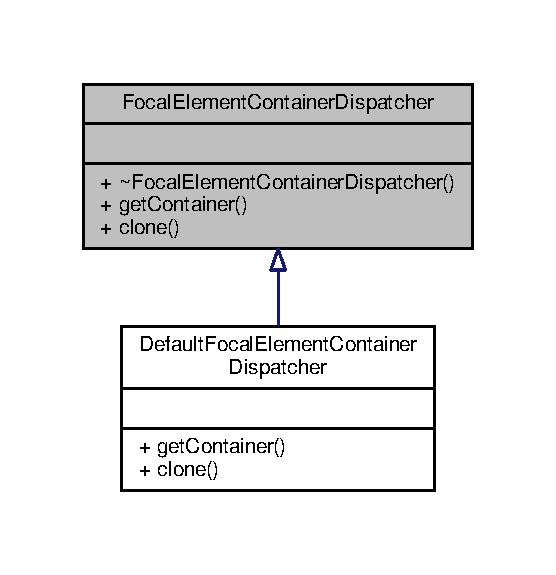
\includegraphics[width=267pt]{classFocalElementContainerDispatcher__inherit__graph}
\end{center}
\end{figure}


Collaboration diagram for Focal\+Element\+Container\+Dispatcher\+:\nopagebreak
\begin{figure}[H]
\begin{center}
\leavevmode
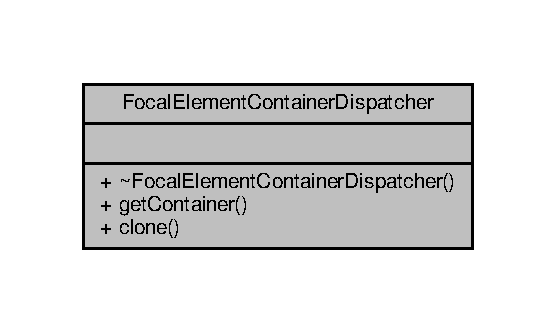
\includegraphics[width=267pt]{classFocalElementContainerDispatcher__coll__graph}
\end{center}
\end{figure}
\subsection*{Public Member Functions}
\begin{DoxyCompactItemize}
\item 
virtual \hyperlink{classFocalElementContainerDispatcher_adc837f38d6ef66d919fc55c9a7933d1b}{$\sim$\+Focal\+Element\+Container\+Dispatcher} ()=default
\item 
virtual std\+::unique\+\_\+ptr$<$ \hyperlink{classFocalElementContainer}{Focal\+Element\+Container} $>$ \hyperlink{classFocalElementContainerDispatcher_af429ae69c47220d55b30cf7e41ee6928}{get\+Container} (const \hyperlink{classFocalElement}{Focal\+Element} \&el)=0
\begin{DoxyCompactList}\small\item\em Get the container given the \hyperlink{classFocalElement}{Focal\+Element} type. \end{DoxyCompactList}\item 
virtual std\+::unique\+\_\+ptr$<$ \hyperlink{classFocalElementContainerDispatcher}{Focal\+Element\+Container\+Dispatcher} $>$ \hyperlink{classFocalElementContainerDispatcher_a710d8bb32947cde2ad5c5e914f33b767}{clone} ()=0
\begin{DoxyCompactList}\small\item\em Clone method. \end{DoxyCompactList}\end{DoxyCompactItemize}


\subsection{Detailed Description}
Dispatcher of the correct \hyperlink{classFocalElementContainer}{Focal\+Element\+Container}, given the \hyperlink{classFocalElement}{Focal\+Element} type. 

\subsection{Constructor \& Destructor Documentation}
\hypertarget{classFocalElementContainerDispatcher_adc837f38d6ef66d919fc55c9a7933d1b}{}\index{Focal\+Element\+Container\+Dispatcher@{Focal\+Element\+Container\+Dispatcher}!````~Focal\+Element\+Container\+Dispatcher@{$\sim$\+Focal\+Element\+Container\+Dispatcher}}
\index{````~Focal\+Element\+Container\+Dispatcher@{$\sim$\+Focal\+Element\+Container\+Dispatcher}!Focal\+Element\+Container\+Dispatcher@{Focal\+Element\+Container\+Dispatcher}}
\subsubsection[{$\sim$\+Focal\+Element\+Container\+Dispatcher}]{\setlength{\rightskip}{0pt plus 5cm}virtual Focal\+Element\+Container\+Dispatcher\+::$\sim$\+Focal\+Element\+Container\+Dispatcher (
\begin{DoxyParamCaption}
{}
\end{DoxyParamCaption}
)\hspace{0.3cm}{\ttfamily [virtual]}, {\ttfamily [default]}}\label{classFocalElementContainerDispatcher_adc837f38d6ef66d919fc55c9a7933d1b}


\subsection{Member Function Documentation}
\hypertarget{classFocalElementContainerDispatcher_a710d8bb32947cde2ad5c5e914f33b767}{}\index{Focal\+Element\+Container\+Dispatcher@{Focal\+Element\+Container\+Dispatcher}!clone@{clone}}
\index{clone@{clone}!Focal\+Element\+Container\+Dispatcher@{Focal\+Element\+Container\+Dispatcher}}
\subsubsection[{clone}]{\setlength{\rightskip}{0pt plus 5cm}virtual std\+::unique\+\_\+ptr$<${\bf Focal\+Element\+Container\+Dispatcher}$>$ Focal\+Element\+Container\+Dispatcher\+::clone (
\begin{DoxyParamCaption}
{}
\end{DoxyParamCaption}
)\hspace{0.3cm}{\ttfamily [pure virtual]}}\label{classFocalElementContainerDispatcher_a710d8bb32947cde2ad5c5e914f33b767}


Clone method. 

\begin{DoxyReturn}{Returns}
A copy of the \hyperlink{classFocalElementContainerDispatcher}{Focal\+Element\+Container\+Dispatcher} object. 
\end{DoxyReturn}


Implemented in \hyperlink{classDefaultFocalElementContainerDispatcher_ac3908e561d7116fdf5b9c6ec9c2b6fdb}{Default\+Focal\+Element\+Container\+Dispatcher}.

\hypertarget{classFocalElementContainerDispatcher_af429ae69c47220d55b30cf7e41ee6928}{}\index{Focal\+Element\+Container\+Dispatcher@{Focal\+Element\+Container\+Dispatcher}!get\+Container@{get\+Container}}
\index{get\+Container@{get\+Container}!Focal\+Element\+Container\+Dispatcher@{Focal\+Element\+Container\+Dispatcher}}
\subsubsection[{get\+Container}]{\setlength{\rightskip}{0pt plus 5cm}virtual std\+::unique\+\_\+ptr$<${\bf Focal\+Element\+Container}$>$ Focal\+Element\+Container\+Dispatcher\+::get\+Container (
\begin{DoxyParamCaption}
\item[{const {\bf Focal\+Element} \&}]{el}
\end{DoxyParamCaption}
)\hspace{0.3cm}{\ttfamily [pure virtual]}}\label{classFocalElementContainerDispatcher_af429ae69c47220d55b30cf7e41ee6928}


Get the container given the \hyperlink{classFocalElement}{Focal\+Element} type. 


\begin{DoxyParams}{Parameters}
{\em el} & Target \hyperlink{classFocalElement}{Focal\+Element} \\
\hline
\end{DoxyParams}
\begin{DoxyReturn}{Returns}
The related \hyperlink{classFocalElementContainer}{Focal\+Element\+Container} 
\end{DoxyReturn}


Implemented in \hyperlink{classDefaultFocalElementContainerDispatcher_a3e2952b8397e02d4ca917e257471781e}{Default\+Focal\+Element\+Container\+Dispatcher}.



The documentation for this class was generated from the following file\+:\begin{DoxyCompactItemize}
\item 
builders/\hyperlink{FocalElementContainerDispatcher_8h}{Focal\+Element\+Container\+Dispatcher.\+h}\end{DoxyCompactItemize}

\hypertarget{classGenericFocalElementContainer}{}\section{Generic\+Focal\+Element\+Container Class Reference}
\label{classGenericFocalElementContainer}\index{Generic\+Focal\+Element\+Container@{Generic\+Focal\+Element\+Container}}


A container for any type of \hyperlink{classFocalElement}{Focal\+Element} object.  




{\ttfamily \#include $<$Generic\+Focal\+Element\+Container.\+h$>$}



Inheritance diagram for Generic\+Focal\+Element\+Container\+:\nopagebreak
\begin{figure}[H]
\begin{center}
\leavevmode
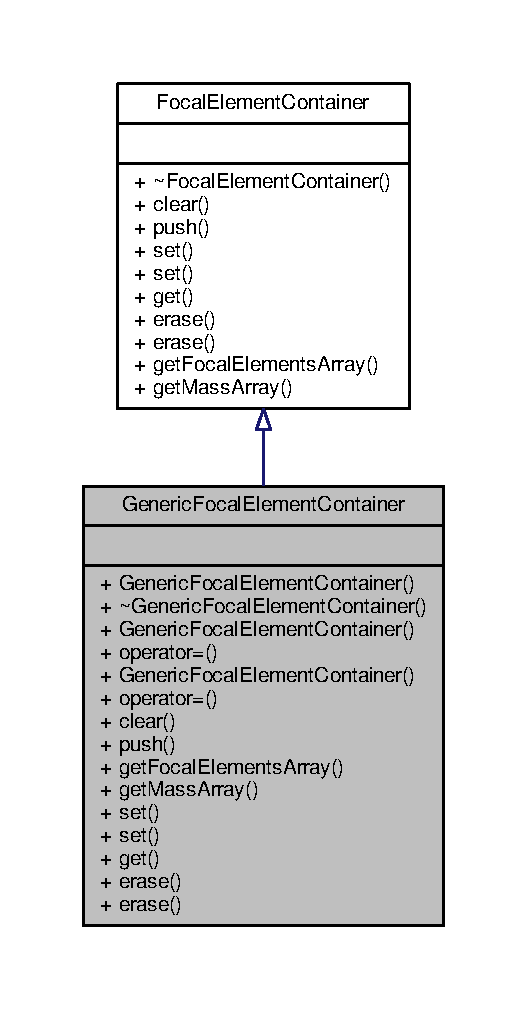
\includegraphics[width=253pt]{classGenericFocalElementContainer__inherit__graph}
\end{center}
\end{figure}


Collaboration diagram for Generic\+Focal\+Element\+Container\+:\nopagebreak
\begin{figure}[H]
\begin{center}
\leavevmode
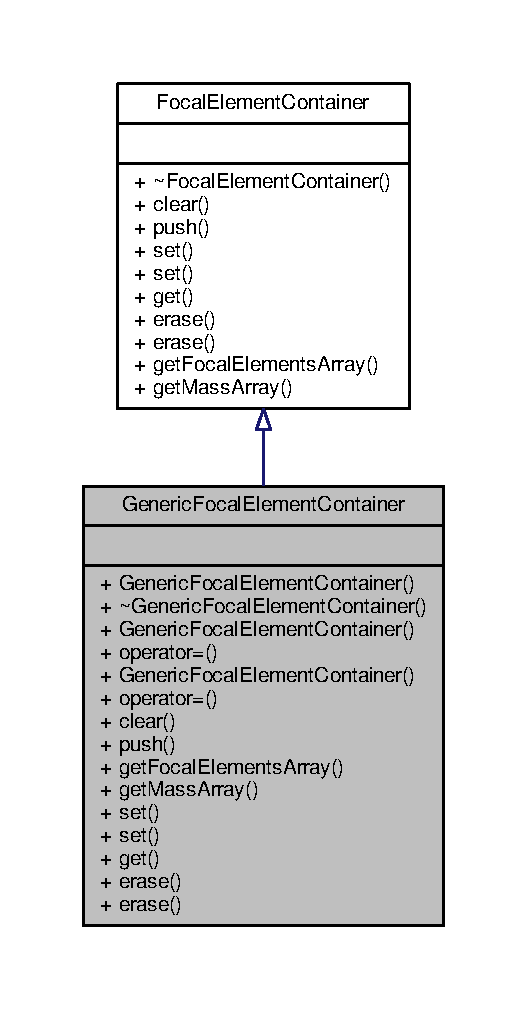
\includegraphics[width=253pt]{classGenericFocalElementContainer__coll__graph}
\end{center}
\end{figure}
\subsection*{Public Member Functions}
\begin{DoxyCompactItemize}
\item 
\hyperlink{classGenericFocalElementContainer_aa8e8154ce9932e6214d865ffc4fa7b60}{Generic\+Focal\+Element\+Container} ()=default
\item 
\hyperlink{classGenericFocalElementContainer_ac93b03b7224ba2163c68201e671e5a1b}{$\sim$\+Generic\+Focal\+Element\+Container} () override=default
\item 
\hyperlink{classGenericFocalElementContainer_ae06b7cfd2004b2c85fe5e92d0d0c0849}{Generic\+Focal\+Element\+Container} (const \hyperlink{classGenericFocalElementContainer}{Generic\+Focal\+Element\+Container} \&other)=delete
\item 
\hyperlink{classGenericFocalElementContainer}{Generic\+Focal\+Element\+Container} \& \hyperlink{classGenericFocalElementContainer_a454c37aa1696dfdbfb9f774edb2c727a}{operator=} (const \hyperlink{classGenericFocalElementContainer}{Generic\+Focal\+Element\+Container} \&other)=delete
\item 
\hyperlink{classGenericFocalElementContainer_a66bf2df46b7897834b4c67b3b8283342}{Generic\+Focal\+Element\+Container} (\hyperlink{classGenericFocalElementContainer}{Generic\+Focal\+Element\+Container} \&\&other)=default
\item 
\hyperlink{classGenericFocalElementContainer}{Generic\+Focal\+Element\+Container} \& \hyperlink{classGenericFocalElementContainer_a206a3e5a1ab891899997e7a9f07987ba}{operator=} (\hyperlink{classGenericFocalElementContainer}{Generic\+Focal\+Element\+Container} \&\&other)=default
\item 
void \hyperlink{classGenericFocalElementContainer_aa20631dceaa742116e6ad6ddf7a38555}{clear} () override
\begin{DoxyCompactList}\small\item\em Clear the container. \end{DoxyCompactList}\item 
void \hyperlink{classGenericFocalElementContainer_aefcc139561645f96f3ec877992005d2b}{push} (std\+::unique\+\_\+ptr$<$ \hyperlink{classFocalElement}{Focal\+Element} $>$ elem, double mass) override
\begin{DoxyCompactList}\small\item\em Add a new \hyperlink{classFocalElement}{Focal\+Element} to the container. \end{DoxyCompactList}\item 
const std\+::vector$<$ std\+::unique\+\_\+ptr$<$ \hyperlink{classFocalElement}{Focal\+Element} $>$ $>$ \& \hyperlink{classGenericFocalElementContainer_a2db442b704235b974d96cd5670ab1630}{get\+Focal\+Elements\+Array} () override
\begin{DoxyCompactList}\small\item\em Get the array of \hyperlink{classFocalElement}{Focal\+Element} object. \end{DoxyCompactList}\item 
const std\+::vector$<$ double $>$ \& \hyperlink{classGenericFocalElementContainer_a0ae8e8ad18f3d8c09db25688f2da684b}{get\+Mass\+Array} () override
\begin{DoxyCompactList}\small\item\em Ge the array of masses. \end{DoxyCompactList}\item 
void \hyperlink{classGenericFocalElementContainer_ae764ae489ed94b366de805a3a45278b9}{set} (int index, double mass) override
\begin{DoxyCompactList}\small\item\em Set the mass value at a given position. \end{DoxyCompactList}\item 
void \hyperlink{classGenericFocalElementContainer_a33d167fa35d3e19ec214560c281681ea}{set} (const \hyperlink{classFocalElement}{Focal\+Element} \&fe, double mass) override
\begin{DoxyCompactList}\small\item\em Set the mass value of the given \hyperlink{classFocalElement}{Focal\+Element}. \end{DoxyCompactList}\item 
double \hyperlink{classGenericFocalElementContainer_a3a9fd25120f480a33770e52d198ecc33}{get} (const \hyperlink{classFocalElement}{Focal\+Element} \&fe) override
\begin{DoxyCompactList}\small\item\em Get the mass value of the given \hyperlink{classFocalElement}{Focal\+Element}. \end{DoxyCompactList}\item 
void \hyperlink{classGenericFocalElementContainer_a123f043d029c636824e4ca8153cd6aea}{erase} (int index) override
\begin{DoxyCompactList}\small\item\em Erase the \hyperlink{classFocalElement}{Focal\+Element} at the given position. \end{DoxyCompactList}\item 
void \hyperlink{classGenericFocalElementContainer_a5bef7f21bc02455dd0cde6dbef69541a}{erase} (const \hyperlink{classFocalElement}{Focal\+Element} \&fe) override
\begin{DoxyCompactList}\small\item\em Erase the given \hyperlink{classFocalElement}{Focal\+Element}. \end{DoxyCompactList}\end{DoxyCompactItemize}


\subsection{Detailed Description}
A container for any type of \hyperlink{classFocalElement}{Focal\+Element} object. 

\subsection{Constructor \& Destructor Documentation}
\hypertarget{classGenericFocalElementContainer_aa8e8154ce9932e6214d865ffc4fa7b60}{}\index{Generic\+Focal\+Element\+Container@{Generic\+Focal\+Element\+Container}!Generic\+Focal\+Element\+Container@{Generic\+Focal\+Element\+Container}}
\index{Generic\+Focal\+Element\+Container@{Generic\+Focal\+Element\+Container}!Generic\+Focal\+Element\+Container@{Generic\+Focal\+Element\+Container}}
\subsubsection[{Generic\+Focal\+Element\+Container}]{\setlength{\rightskip}{0pt plus 5cm}Generic\+Focal\+Element\+Container\+::\+Generic\+Focal\+Element\+Container (
\begin{DoxyParamCaption}
{}
\end{DoxyParamCaption}
)\hspace{0.3cm}{\ttfamily [default]}}\label{classGenericFocalElementContainer_aa8e8154ce9932e6214d865ffc4fa7b60}
\hypertarget{classGenericFocalElementContainer_ac93b03b7224ba2163c68201e671e5a1b}{}\index{Generic\+Focal\+Element\+Container@{Generic\+Focal\+Element\+Container}!````~Generic\+Focal\+Element\+Container@{$\sim$\+Generic\+Focal\+Element\+Container}}
\index{````~Generic\+Focal\+Element\+Container@{$\sim$\+Generic\+Focal\+Element\+Container}!Generic\+Focal\+Element\+Container@{Generic\+Focal\+Element\+Container}}
\subsubsection[{$\sim$\+Generic\+Focal\+Element\+Container}]{\setlength{\rightskip}{0pt plus 5cm}Generic\+Focal\+Element\+Container\+::$\sim$\+Generic\+Focal\+Element\+Container (
\begin{DoxyParamCaption}
{}
\end{DoxyParamCaption}
)\hspace{0.3cm}{\ttfamily [override]}, {\ttfamily [default]}}\label{classGenericFocalElementContainer_ac93b03b7224ba2163c68201e671e5a1b}
\hypertarget{classGenericFocalElementContainer_ae06b7cfd2004b2c85fe5e92d0d0c0849}{}\index{Generic\+Focal\+Element\+Container@{Generic\+Focal\+Element\+Container}!Generic\+Focal\+Element\+Container@{Generic\+Focal\+Element\+Container}}
\index{Generic\+Focal\+Element\+Container@{Generic\+Focal\+Element\+Container}!Generic\+Focal\+Element\+Container@{Generic\+Focal\+Element\+Container}}
\subsubsection[{Generic\+Focal\+Element\+Container}]{\setlength{\rightskip}{0pt plus 5cm}Generic\+Focal\+Element\+Container\+::\+Generic\+Focal\+Element\+Container (
\begin{DoxyParamCaption}
\item[{const {\bf Generic\+Focal\+Element\+Container} \&}]{other}
\end{DoxyParamCaption}
)\hspace{0.3cm}{\ttfamily [delete]}}\label{classGenericFocalElementContainer_ae06b7cfd2004b2c85fe5e92d0d0c0849}
\hypertarget{classGenericFocalElementContainer_a66bf2df46b7897834b4c67b3b8283342}{}\index{Generic\+Focal\+Element\+Container@{Generic\+Focal\+Element\+Container}!Generic\+Focal\+Element\+Container@{Generic\+Focal\+Element\+Container}}
\index{Generic\+Focal\+Element\+Container@{Generic\+Focal\+Element\+Container}!Generic\+Focal\+Element\+Container@{Generic\+Focal\+Element\+Container}}
\subsubsection[{Generic\+Focal\+Element\+Container}]{\setlength{\rightskip}{0pt plus 5cm}Generic\+Focal\+Element\+Container\+::\+Generic\+Focal\+Element\+Container (
\begin{DoxyParamCaption}
\item[{{\bf Generic\+Focal\+Element\+Container} \&\&}]{other}
\end{DoxyParamCaption}
)\hspace{0.3cm}{\ttfamily [default]}}\label{classGenericFocalElementContainer_a66bf2df46b7897834b4c67b3b8283342}


\subsection{Member Function Documentation}
\hypertarget{classGenericFocalElementContainer_aa20631dceaa742116e6ad6ddf7a38555}{}\index{Generic\+Focal\+Element\+Container@{Generic\+Focal\+Element\+Container}!clear@{clear}}
\index{clear@{clear}!Generic\+Focal\+Element\+Container@{Generic\+Focal\+Element\+Container}}
\subsubsection[{clear}]{\setlength{\rightskip}{0pt plus 5cm}void Generic\+Focal\+Element\+Container\+::clear (
\begin{DoxyParamCaption}
{}
\end{DoxyParamCaption}
)\hspace{0.3cm}{\ttfamily [override]}, {\ttfamily [virtual]}}\label{classGenericFocalElementContainer_aa20631dceaa742116e6ad6ddf7a38555}


Clear the container. 



Implements \hyperlink{classFocalElementContainer_a79977845eba147c3d29d8c500dbe593c}{Focal\+Element\+Container}.

\hypertarget{classGenericFocalElementContainer_a123f043d029c636824e4ca8153cd6aea}{}\index{Generic\+Focal\+Element\+Container@{Generic\+Focal\+Element\+Container}!erase@{erase}}
\index{erase@{erase}!Generic\+Focal\+Element\+Container@{Generic\+Focal\+Element\+Container}}
\subsubsection[{erase}]{\setlength{\rightskip}{0pt plus 5cm}void Generic\+Focal\+Element\+Container\+::erase (
\begin{DoxyParamCaption}
\item[{int}]{index}
\end{DoxyParamCaption}
)\hspace{0.3cm}{\ttfamily [override]}, {\ttfamily [virtual]}}\label{classGenericFocalElementContainer_a123f043d029c636824e4ca8153cd6aea}


Erase the \hyperlink{classFocalElement}{Focal\+Element} at the given position. 


\begin{DoxyParams}{Parameters}
{\em index} & The target position. \\
\hline
\end{DoxyParams}


Implements \hyperlink{classFocalElementContainer_aaf91ad85eeb5b218171a142d7c3e1116}{Focal\+Element\+Container}.

\hypertarget{classGenericFocalElementContainer_a5bef7f21bc02455dd0cde6dbef69541a}{}\index{Generic\+Focal\+Element\+Container@{Generic\+Focal\+Element\+Container}!erase@{erase}}
\index{erase@{erase}!Generic\+Focal\+Element\+Container@{Generic\+Focal\+Element\+Container}}
\subsubsection[{erase}]{\setlength{\rightskip}{0pt plus 5cm}void Generic\+Focal\+Element\+Container\+::erase (
\begin{DoxyParamCaption}
\item[{const {\bf Focal\+Element} \&}]{fe}
\end{DoxyParamCaption}
)\hspace{0.3cm}{\ttfamily [override]}, {\ttfamily [virtual]}}\label{classGenericFocalElementContainer_a5bef7f21bc02455dd0cde6dbef69541a}


Erase the given \hyperlink{classFocalElement}{Focal\+Element}. 


\begin{DoxyParams}{Parameters}
{\em fe} & The target \hyperlink{classFocalElement}{Focal\+Element}. \\
\hline
\end{DoxyParams}


Implements \hyperlink{classFocalElementContainer_af20780adab46a8d4e5b42c8b1934ea86}{Focal\+Element\+Container}.

\hypertarget{classGenericFocalElementContainer_a3a9fd25120f480a33770e52d198ecc33}{}\index{Generic\+Focal\+Element\+Container@{Generic\+Focal\+Element\+Container}!get@{get}}
\index{get@{get}!Generic\+Focal\+Element\+Container@{Generic\+Focal\+Element\+Container}}
\subsubsection[{get}]{\setlength{\rightskip}{0pt plus 5cm}double Generic\+Focal\+Element\+Container\+::get (
\begin{DoxyParamCaption}
\item[{const {\bf Focal\+Element} \&}]{fe}
\end{DoxyParamCaption}
)\hspace{0.3cm}{\ttfamily [override]}, {\ttfamily [virtual]}}\label{classGenericFocalElementContainer_a3a9fd25120f480a33770e52d198ecc33}


Get the mass value of the given \hyperlink{classFocalElement}{Focal\+Element}. 


\begin{DoxyParams}{Parameters}
{\em fe} & The target \hyperlink{classFocalElement}{Focal\+Element} \\
\hline
\end{DoxyParams}
\begin{DoxyReturn}{Returns}
The associated mass value 
\end{DoxyReturn}


Implements \hyperlink{classFocalElementContainer_a5ffaa25475069d4868cec5a73ccf314f}{Focal\+Element\+Container}.

\hypertarget{classGenericFocalElementContainer_a2db442b704235b974d96cd5670ab1630}{}\index{Generic\+Focal\+Element\+Container@{Generic\+Focal\+Element\+Container}!get\+Focal\+Elements\+Array@{get\+Focal\+Elements\+Array}}
\index{get\+Focal\+Elements\+Array@{get\+Focal\+Elements\+Array}!Generic\+Focal\+Element\+Container@{Generic\+Focal\+Element\+Container}}
\subsubsection[{get\+Focal\+Elements\+Array}]{\setlength{\rightskip}{0pt plus 5cm}const std\+::vector$<$ std\+::unique\+\_\+ptr$<$ {\bf Focal\+Element} $>$ $>$ \& Generic\+Focal\+Element\+Container\+::get\+Focal\+Elements\+Array (
\begin{DoxyParamCaption}
{}
\end{DoxyParamCaption}
)\hspace{0.3cm}{\ttfamily [override]}, {\ttfamily [virtual]}}\label{classGenericFocalElementContainer_a2db442b704235b974d96cd5670ab1630}


Get the array of \hyperlink{classFocalElement}{Focal\+Element} object. 

\begin{DoxyReturn}{Returns}
Array of \hyperlink{classFocalElement}{Focal\+Element}. 
\end{DoxyReturn}


Implements \hyperlink{classFocalElementContainer_aa06ed4c0c21777cdc5256b576dc5e718}{Focal\+Element\+Container}.

\hypertarget{classGenericFocalElementContainer_a0ae8e8ad18f3d8c09db25688f2da684b}{}\index{Generic\+Focal\+Element\+Container@{Generic\+Focal\+Element\+Container}!get\+Mass\+Array@{get\+Mass\+Array}}
\index{get\+Mass\+Array@{get\+Mass\+Array}!Generic\+Focal\+Element\+Container@{Generic\+Focal\+Element\+Container}}
\subsubsection[{get\+Mass\+Array}]{\setlength{\rightskip}{0pt plus 5cm}const std\+::vector$<$ double $>$ \& Generic\+Focal\+Element\+Container\+::get\+Mass\+Array (
\begin{DoxyParamCaption}
{}
\end{DoxyParamCaption}
)\hspace{0.3cm}{\ttfamily [override]}, {\ttfamily [virtual]}}\label{classGenericFocalElementContainer_a0ae8e8ad18f3d8c09db25688f2da684b}


Ge the array of masses. 

\begin{DoxyReturn}{Returns}
Array of masses. 
\end{DoxyReturn}


Implements \hyperlink{classFocalElementContainer_a9197229964bfdf8765f81bf7b85c669d}{Focal\+Element\+Container}.

\hypertarget{classGenericFocalElementContainer_a454c37aa1696dfdbfb9f774edb2c727a}{}\index{Generic\+Focal\+Element\+Container@{Generic\+Focal\+Element\+Container}!operator=@{operator=}}
\index{operator=@{operator=}!Generic\+Focal\+Element\+Container@{Generic\+Focal\+Element\+Container}}
\subsubsection[{operator=}]{\setlength{\rightskip}{0pt plus 5cm}{\bf Generic\+Focal\+Element\+Container}\& Generic\+Focal\+Element\+Container\+::operator= (
\begin{DoxyParamCaption}
\item[{const {\bf Generic\+Focal\+Element\+Container} \&}]{other}
\end{DoxyParamCaption}
)\hspace{0.3cm}{\ttfamily [delete]}}\label{classGenericFocalElementContainer_a454c37aa1696dfdbfb9f774edb2c727a}
\hypertarget{classGenericFocalElementContainer_a206a3e5a1ab891899997e7a9f07987ba}{}\index{Generic\+Focal\+Element\+Container@{Generic\+Focal\+Element\+Container}!operator=@{operator=}}
\index{operator=@{operator=}!Generic\+Focal\+Element\+Container@{Generic\+Focal\+Element\+Container}}
\subsubsection[{operator=}]{\setlength{\rightskip}{0pt plus 5cm}{\bf Generic\+Focal\+Element\+Container}\& Generic\+Focal\+Element\+Container\+::operator= (
\begin{DoxyParamCaption}
\item[{{\bf Generic\+Focal\+Element\+Container} \&\&}]{other}
\end{DoxyParamCaption}
)\hspace{0.3cm}{\ttfamily [default]}}\label{classGenericFocalElementContainer_a206a3e5a1ab891899997e7a9f07987ba}
\hypertarget{classGenericFocalElementContainer_aefcc139561645f96f3ec877992005d2b}{}\index{Generic\+Focal\+Element\+Container@{Generic\+Focal\+Element\+Container}!push@{push}}
\index{push@{push}!Generic\+Focal\+Element\+Container@{Generic\+Focal\+Element\+Container}}
\subsubsection[{push}]{\setlength{\rightskip}{0pt plus 5cm}void Generic\+Focal\+Element\+Container\+::push (
\begin{DoxyParamCaption}
\item[{std\+::unique\+\_\+ptr$<$ {\bf Focal\+Element} $>$}]{elem, }
\item[{double}]{mass}
\end{DoxyParamCaption}
)\hspace{0.3cm}{\ttfamily [override]}, {\ttfamily [virtual]}}\label{classGenericFocalElementContainer_aefcc139561645f96f3ec877992005d2b}


Add a new \hyperlink{classFocalElement}{Focal\+Element} to the container. 


\begin{DoxyParams}{Parameters}
{\em elem} & The \hyperlink{classFocalElement}{Focal\+Element} to be added. \\
\hline
{\em mass} & The mass value. \\
\hline
\end{DoxyParams}


Implements \hyperlink{classFocalElementContainer_a951895e83f8ef4ba79fa1c45d2d3c1ac}{Focal\+Element\+Container}.

\hypertarget{classGenericFocalElementContainer_ae764ae489ed94b366de805a3a45278b9}{}\index{Generic\+Focal\+Element\+Container@{Generic\+Focal\+Element\+Container}!set@{set}}
\index{set@{set}!Generic\+Focal\+Element\+Container@{Generic\+Focal\+Element\+Container}}
\subsubsection[{set}]{\setlength{\rightskip}{0pt plus 5cm}void Generic\+Focal\+Element\+Container\+::set (
\begin{DoxyParamCaption}
\item[{int}]{index, }
\item[{double}]{mass}
\end{DoxyParamCaption}
)\hspace{0.3cm}{\ttfamily [override]}, {\ttfamily [virtual]}}\label{classGenericFocalElementContainer_ae764ae489ed94b366de805a3a45278b9}


Set the mass value at a given position. 


\begin{DoxyParams}{Parameters}
{\em index} & The target position. \\
\hline
{\em mass} & The new mass value. \\
\hline
\end{DoxyParams}


Implements \hyperlink{classFocalElementContainer_a37edfcf750dfc72a7f3a92a2ab6bd62e}{Focal\+Element\+Container}.

\hypertarget{classGenericFocalElementContainer_a33d167fa35d3e19ec214560c281681ea}{}\index{Generic\+Focal\+Element\+Container@{Generic\+Focal\+Element\+Container}!set@{set}}
\index{set@{set}!Generic\+Focal\+Element\+Container@{Generic\+Focal\+Element\+Container}}
\subsubsection[{set}]{\setlength{\rightskip}{0pt plus 5cm}void Generic\+Focal\+Element\+Container\+::set (
\begin{DoxyParamCaption}
\item[{const {\bf Focal\+Element} \&}]{fe, }
\item[{double}]{mass}
\end{DoxyParamCaption}
)\hspace{0.3cm}{\ttfamily [override]}, {\ttfamily [virtual]}}\label{classGenericFocalElementContainer_a33d167fa35d3e19ec214560c281681ea}


Set the mass value of the given \hyperlink{classFocalElement}{Focal\+Element}. 


\begin{DoxyParams}{Parameters}
{\em fe} & The target \hyperlink{classFocalElement}{Focal\+Element}. \\
\hline
{\em mass} & The new mass value. \\
\hline
\end{DoxyParams}


Implements \hyperlink{classFocalElementContainer_a444a088fc937650226f2ecdd1db59510}{Focal\+Element\+Container}.



The documentation for this class was generated from the following files\+:\begin{DoxyCompactItemize}
\item 
builders/\hyperlink{GenericFocalElementContainer_8h}{Generic\+Focal\+Element\+Container.\+h}\item 
builders/\hyperlink{GenericFocalElementContainer_8cpp}{Generic\+Focal\+Element\+Container.\+cpp}\end{DoxyCompactItemize}

\hypertarget{classstd_1_1hash_3_01std_1_1unique__ptr_3_01HashableFocalElement_01_4_01_4}{}\section{std\+:\+:hash$<$ std\+:\+:unique\+\_\+ptr$<$ Hashable\+Focal\+Element $>$ $>$ Class Template Reference}
\label{classstd_1_1hash_3_01std_1_1unique__ptr_3_01HashableFocalElement_01_4_01_4}\index{std\+::hash$<$ std\+::unique\+\_\+ptr$<$ Hashable\+Focal\+Element $>$ $>$@{std\+::hash$<$ std\+::unique\+\_\+ptr$<$ Hashable\+Focal\+Element $>$ $>$}}


{\ttfamily \#include $<$Hashable\+Focal\+Element.\+h$>$}



Collaboration diagram for std\+:\+:hash$<$ std\+:\+:unique\+\_\+ptr$<$ Hashable\+Focal\+Element $>$ $>$\+:\nopagebreak
\begin{figure}[H]
\begin{center}
\leavevmode
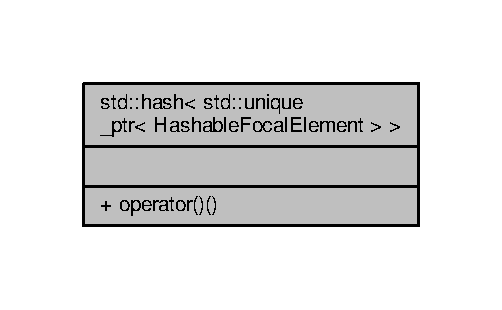
\includegraphics[width=241pt]{classstd_1_1hash_3_01std_1_1unique__ptr_3_01HashableFocalElement_01_4_01_4__coll__graph}
\end{center}
\end{figure}
\subsection*{Public Member Functions}
\begin{DoxyCompactItemize}
\item 
size\+\_\+t \hyperlink{classstd_1_1hash_3_01std_1_1unique__ptr_3_01HashableFocalElement_01_4_01_4_a7625821524070a3c3be03dc6701d30c4}{operator()} (const std\+::unique\+\_\+ptr$<$ \hyperlink{classHashableFocalElement}{Hashable\+Focal\+Element} $>$ \&fe) const 
\end{DoxyCompactItemize}


\subsection{Member Function Documentation}
\hypertarget{classstd_1_1hash_3_01std_1_1unique__ptr_3_01HashableFocalElement_01_4_01_4_a7625821524070a3c3be03dc6701d30c4}{}\index{std\+::hash$<$ std\+::unique\+\_\+ptr$<$ Hashable\+Focal\+Element $>$ $>$@{std\+::hash$<$ std\+::unique\+\_\+ptr$<$ Hashable\+Focal\+Element $>$ $>$}!operator()@{operator()}}
\index{operator()@{operator()}!std\+::hash$<$ std\+::unique\+\_\+ptr$<$ Hashable\+Focal\+Element $>$ $>$@{std\+::hash$<$ std\+::unique\+\_\+ptr$<$ Hashable\+Focal\+Element $>$ $>$}}
\subsubsection[{operator()}]{\setlength{\rightskip}{0pt plus 5cm}size\+\_\+t std\+::hash$<$ std\+::unique\+\_\+ptr$<$ {\bf Hashable\+Focal\+Element} $>$ $>$\+::operator() (
\begin{DoxyParamCaption}
\item[{const std\+::unique\+\_\+ptr$<$ {\bf Hashable\+Focal\+Element} $>$ \&}]{fe}
\end{DoxyParamCaption}
) const\hspace{0.3cm}{\ttfamily [inline]}}\label{classstd_1_1hash_3_01std_1_1unique__ptr_3_01HashableFocalElement_01_4_01_4_a7625821524070a3c3be03dc6701d30c4}


The documentation for this class was generated from the following file\+:\begin{DoxyCompactItemize}
\item 
focal\+\_\+elements/\hyperlink{HashableFocalElement_8h}{Hashable\+Focal\+Element.\+h}\end{DoxyCompactItemize}

\hypertarget{classHashableFocalElement}{}\section{Hashable\+Focal\+Element Class Reference}
\label{classHashableFocalElement}\index{Hashable\+Focal\+Element@{Hashable\+Focal\+Element}}


{\ttfamily \#include $<$Hashable\+Focal\+Element.\+h$>$}



Inheritance diagram for Hashable\+Focal\+Element\+:\nopagebreak
\begin{figure}[H]
\begin{center}
\leavevmode
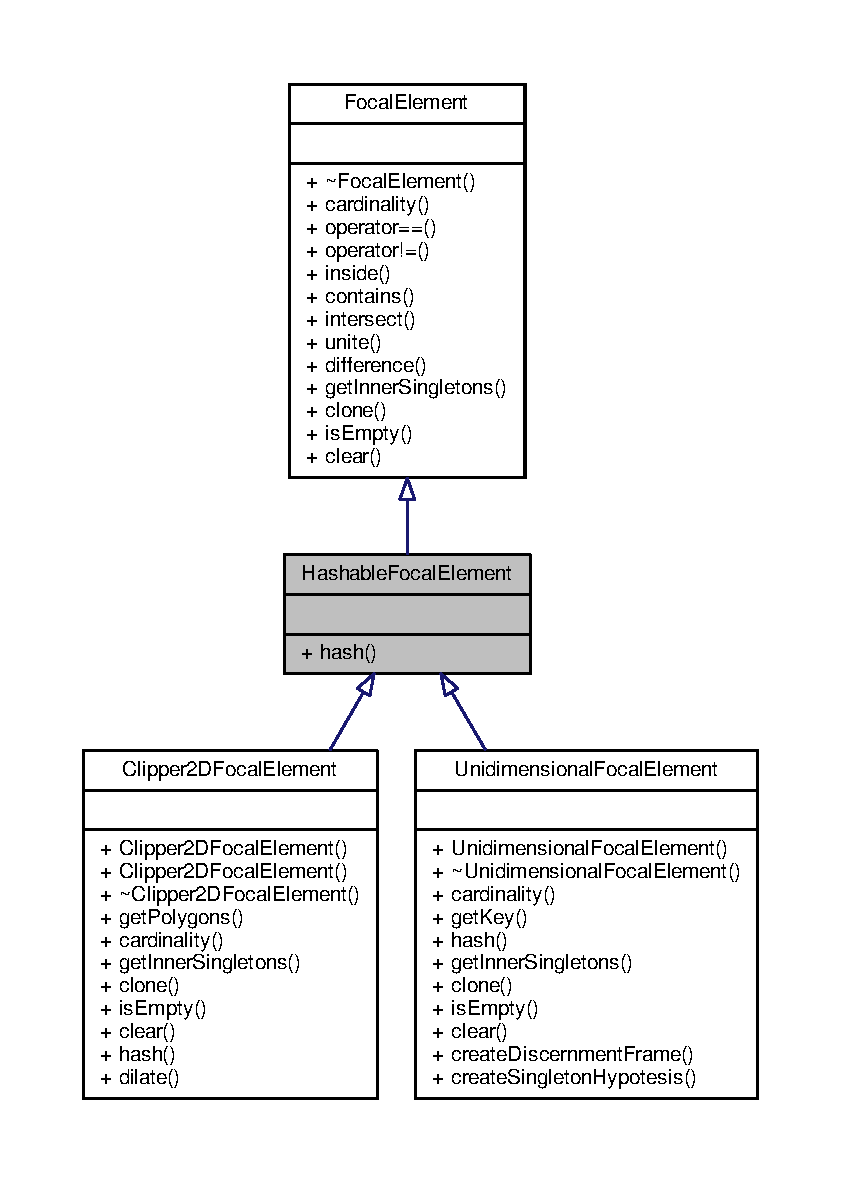
\includegraphics[height=550pt]{classHashableFocalElement__inherit__graph}
\end{center}
\end{figure}


Collaboration diagram for Hashable\+Focal\+Element\+:\nopagebreak
\begin{figure}[H]
\begin{center}
\leavevmode
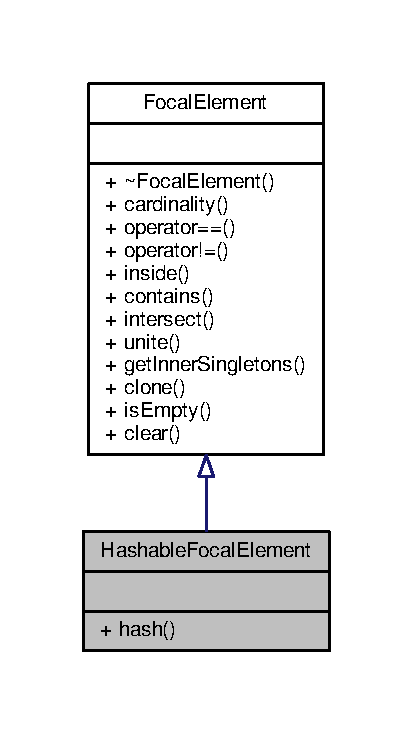
\includegraphics[width=198pt]{classHashableFocalElement__coll__graph}
\end{center}
\end{figure}
\subsection*{Public Member Functions}
\begin{DoxyCompactItemize}
\item 
virtual size\+\_\+t \hyperlink{classHashableFocalElement_a8b7bfbf1e107fa5a6cfc5033db196c63}{hash} () const =0
\end{DoxyCompactItemize}


\subsection{Member Function Documentation}
\hypertarget{classHashableFocalElement_a8b7bfbf1e107fa5a6cfc5033db196c63}{}\index{Hashable\+Focal\+Element@{Hashable\+Focal\+Element}!hash@{hash}}
\index{hash@{hash}!Hashable\+Focal\+Element@{Hashable\+Focal\+Element}}
\subsubsection[{hash}]{\setlength{\rightskip}{0pt plus 5cm}virtual size\+\_\+t Hashable\+Focal\+Element\+::hash (
\begin{DoxyParamCaption}
{}
\end{DoxyParamCaption}
) const\hspace{0.3cm}{\ttfamily [pure virtual]}}\label{classHashableFocalElement_a8b7bfbf1e107fa5a6cfc5033db196c63}


Implemented in \hyperlink{classUnidimensionalFocalElement_a073ce6e51cb7fff32b53e5f7b1d729c7}{Unidimensional\+Focal\+Element}.



The documentation for this class was generated from the following file\+:\begin{DoxyCompactItemize}
\item 
focal\+\_\+elements/\hyperlink{HashableFocalElement_8h}{Hashable\+Focal\+Element.\+h}\end{DoxyCompactItemize}

\hypertarget{classHashableFocalElementContainer}{}\section{Hashable\+Focal\+Element\+Container Class Reference}
\label{classHashableFocalElementContainer}\index{Hashable\+Focal\+Element\+Container@{Hashable\+Focal\+Element\+Container}}


A container for \hyperlink{classHashableFocalElement}{Hashable\+Focal\+Element} type objects.  




{\ttfamily \#include $<$Hashable\+Focal\+Element\+Container.\+h$>$}



Inheritance diagram for Hashable\+Focal\+Element\+Container\+:\nopagebreak
\begin{figure}[H]
\begin{center}
\leavevmode
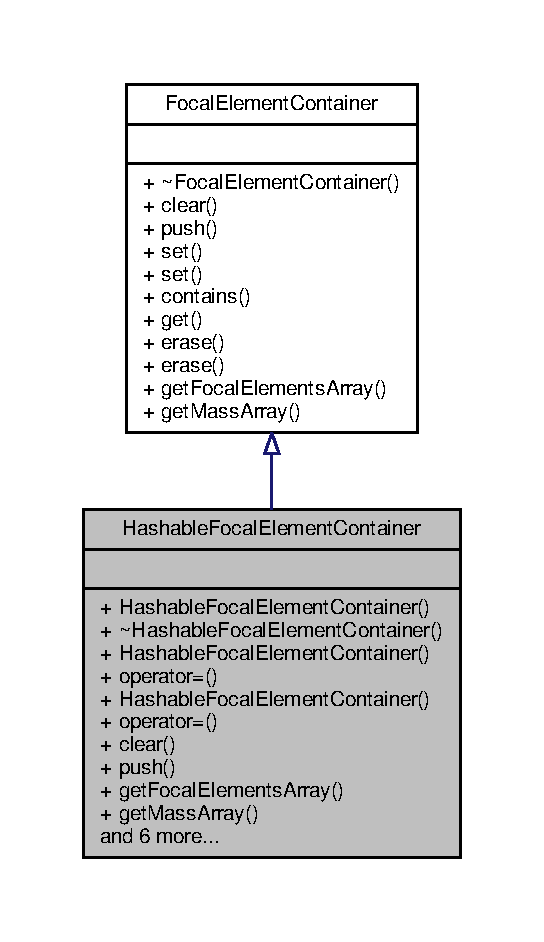
\includegraphics[width=261pt]{classHashableFocalElementContainer__inherit__graph}
\end{center}
\end{figure}


Collaboration diagram for Hashable\+Focal\+Element\+Container\+:\nopagebreak
\begin{figure}[H]
\begin{center}
\leavevmode
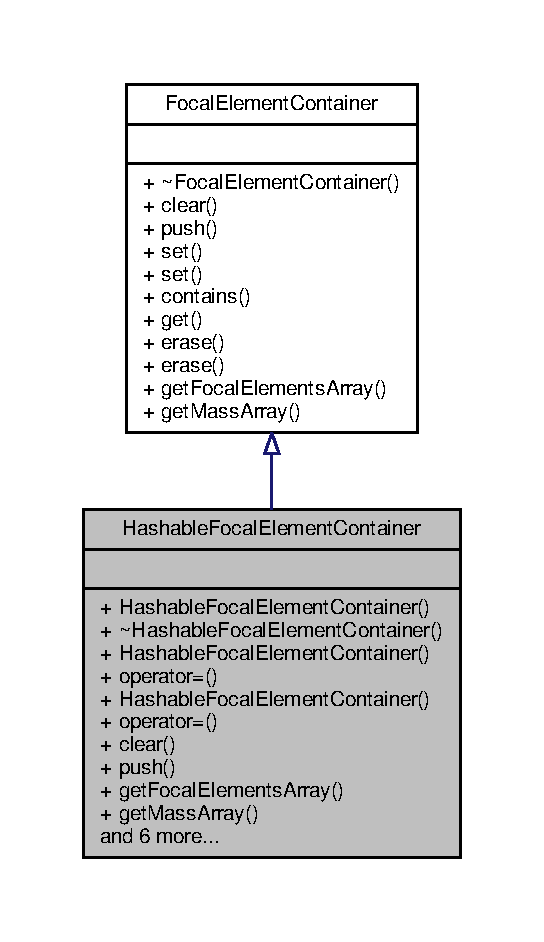
\includegraphics[width=261pt]{classHashableFocalElementContainer__coll__graph}
\end{center}
\end{figure}
\subsection*{Public Member Functions}
\begin{DoxyCompactItemize}
\item 
\hyperlink{classHashableFocalElementContainer_a59ef0e4b071a31c9ec4d12b265966459}{Hashable\+Focal\+Element\+Container} ()=default
\item 
\hyperlink{classHashableFocalElementContainer_a105af5bcdf825c1ac55b2d36abe691eb}{$\sim$\+Hashable\+Focal\+Element\+Container} () override=default
\item 
\hyperlink{classHashableFocalElementContainer_a45b0628e9bd91e6f2bd0c574e7958579}{Hashable\+Focal\+Element\+Container} (const \hyperlink{classHashableFocalElementContainer}{Hashable\+Focal\+Element\+Container} \&other)=delete
\item 
\hyperlink{classHashableFocalElementContainer}{Hashable\+Focal\+Element\+Container} \& \hyperlink{classHashableFocalElementContainer_aa1e05287cf51b5480ba4ec7f8a63476d}{operator=} (const \hyperlink{classHashableFocalElementContainer}{Hashable\+Focal\+Element\+Container} \&other)=delete
\item 
\hyperlink{classHashableFocalElementContainer_acbb66df9fd4caec000da0d07957192dc}{Hashable\+Focal\+Element\+Container} (\hyperlink{classHashableFocalElementContainer}{Hashable\+Focal\+Element\+Container} \&\&other)=default
\item 
\hyperlink{classHashableFocalElementContainer}{Hashable\+Focal\+Element\+Container} \& \hyperlink{classHashableFocalElementContainer_ad66a0f24eb49efdc08450d0885c6de9e}{operator=} (\hyperlink{classHashableFocalElementContainer}{Hashable\+Focal\+Element\+Container} \&\&other)=default
\item 
void \hyperlink{classHashableFocalElementContainer_a352c7bc7f6b705bd1a5d5e5b9ec225fe}{clear} () override
\begin{DoxyCompactList}\small\item\em Clear the container. \end{DoxyCompactList}\item 
void \hyperlink{classHashableFocalElementContainer_a896a7b5c2719e63b1ad8a53a6d33c6c7}{push} (std\+::unique\+\_\+ptr$<$ \hyperlink{classFocalElement}{Focal\+Element} $>$ elem, double mass) override
\begin{DoxyCompactList}\small\item\em Add a new \hyperlink{classFocalElement}{Focal\+Element} to the container. \end{DoxyCompactList}\item 
const std\+::vector$<$ std\+::unique\+\_\+ptr$<$ \hyperlink{classFocalElement}{Focal\+Element} $>$ $>$ \& \hyperlink{classHashableFocalElementContainer_a11ab286119f448d1a480dd4336875b9f}{get\+Focal\+Elements\+Array} () override
\begin{DoxyCompactList}\small\item\em Get the array of \hyperlink{classFocalElement}{Focal\+Element} object. \end{DoxyCompactList}\item 
const std\+::vector$<$ double $>$ \& \hyperlink{classHashableFocalElementContainer_a8be85b980960704d31563d0ad64b8aad}{get\+Mass\+Array} () override
\begin{DoxyCompactList}\small\item\em Ge the array of masses. \end{DoxyCompactList}\item 
void \hyperlink{classHashableFocalElementContainer_a95613540899807e8094f39f75f92e088}{set} (\hyperlink{CMakeCache_8txt_a79a3d8790b2588b09777910863574e09}{int} index, double mass) override
\begin{DoxyCompactList}\small\item\em Set the mass value at a given position. \end{DoxyCompactList}\item 
void \hyperlink{classHashableFocalElementContainer_a16ac0c831312f31641aa716b19a3efed}{set} (const \hyperlink{classFocalElement}{Focal\+Element} \&fe, double mass) override
\begin{DoxyCompactList}\small\item\em Set the mass value of the given \hyperlink{classFocalElement}{Focal\+Element}. \end{DoxyCompactList}\item 
double \hyperlink{classHashableFocalElementContainer_a0b384b37bee91526a932756a65727be0}{get} (const \hyperlink{classFocalElement}{Focal\+Element} \&fe) override
\begin{DoxyCompactList}\small\item\em Get the mass value of the given \hyperlink{classFocalElement}{Focal\+Element}. \end{DoxyCompactList}\item 
void \hyperlink{classHashableFocalElementContainer_a06450d7d5174bdeecd2238570143e2b3}{erase} (\hyperlink{CMakeCache_8txt_a79a3d8790b2588b09777910863574e09}{int} index) override
\begin{DoxyCompactList}\small\item\em Erase the \hyperlink{classFocalElement}{Focal\+Element} at the given position. \end{DoxyCompactList}\item 
void \hyperlink{classHashableFocalElementContainer_a8d072157c5715b764e3158427157a242}{erase} (const \hyperlink{classFocalElement}{Focal\+Element} \&fe) override
\begin{DoxyCompactList}\small\item\em Erase the given \hyperlink{classFocalElement}{Focal\+Element}. \end{DoxyCompactList}\item 
bool \hyperlink{classHashableFocalElementContainer_a3c359b0257b7e03d1d0fe10d7bc35bd3}{contains} (const \hyperlink{classFocalElement}{Focal\+Element} \&fe) override
\begin{DoxyCompactList}\small\item\em Returns true if the given \hyperlink{classFocalElement}{Focal\+Element} is inside the container. \end{DoxyCompactList}\end{DoxyCompactItemize}


\subsection{Detailed Description}
A container for \hyperlink{classHashableFocalElement}{Hashable\+Focal\+Element} type objects. 

\subsection{Constructor \& Destructor Documentation}
\index{Hashable\+Focal\+Element\+Container@{Hashable\+Focal\+Element\+Container}!Hashable\+Focal\+Element\+Container@{Hashable\+Focal\+Element\+Container}}
\index{Hashable\+Focal\+Element\+Container@{Hashable\+Focal\+Element\+Container}!Hashable\+Focal\+Element\+Container@{Hashable\+Focal\+Element\+Container}}
\subsubsection[{\texorpdfstring{Hashable\+Focal\+Element\+Container()=default}{HashableFocalElementContainer()=default}}]{\setlength{\rightskip}{0pt plus 5cm}Hashable\+Focal\+Element\+Container\+::\+Hashable\+Focal\+Element\+Container (
\begin{DoxyParamCaption}
{}
\end{DoxyParamCaption}
)\hspace{0.3cm}{\ttfamily [default]}}\hypertarget{classHashableFocalElementContainer_a59ef0e4b071a31c9ec4d12b265966459}{}\label{classHashableFocalElementContainer_a59ef0e4b071a31c9ec4d12b265966459}
\index{Hashable\+Focal\+Element\+Container@{Hashable\+Focal\+Element\+Container}!````~Hashable\+Focal\+Element\+Container@{$\sim$\+Hashable\+Focal\+Element\+Container}}
\index{````~Hashable\+Focal\+Element\+Container@{$\sim$\+Hashable\+Focal\+Element\+Container}!Hashable\+Focal\+Element\+Container@{Hashable\+Focal\+Element\+Container}}
\subsubsection[{\texorpdfstring{$\sim$\+Hashable\+Focal\+Element\+Container() override=default}{~HashableFocalElementContainer() override=default}}]{\setlength{\rightskip}{0pt plus 5cm}Hashable\+Focal\+Element\+Container\+::$\sim$\+Hashable\+Focal\+Element\+Container (
\begin{DoxyParamCaption}
{}
\end{DoxyParamCaption}
)\hspace{0.3cm}{\ttfamily [override]}, {\ttfamily [default]}}\hypertarget{classHashableFocalElementContainer_a105af5bcdf825c1ac55b2d36abe691eb}{}\label{classHashableFocalElementContainer_a105af5bcdf825c1ac55b2d36abe691eb}
\index{Hashable\+Focal\+Element\+Container@{Hashable\+Focal\+Element\+Container}!Hashable\+Focal\+Element\+Container@{Hashable\+Focal\+Element\+Container}}
\index{Hashable\+Focal\+Element\+Container@{Hashable\+Focal\+Element\+Container}!Hashable\+Focal\+Element\+Container@{Hashable\+Focal\+Element\+Container}}
\subsubsection[{\texorpdfstring{Hashable\+Focal\+Element\+Container(const Hashable\+Focal\+Element\+Container \&other)=delete}{HashableFocalElementContainer(const HashableFocalElementContainer &other)=delete}}]{\setlength{\rightskip}{0pt plus 5cm}Hashable\+Focal\+Element\+Container\+::\+Hashable\+Focal\+Element\+Container (
\begin{DoxyParamCaption}
\item[{const {\bf Hashable\+Focal\+Element\+Container} \&}]{other}
\end{DoxyParamCaption}
)\hspace{0.3cm}{\ttfamily [delete]}}\hypertarget{classHashableFocalElementContainer_a45b0628e9bd91e6f2bd0c574e7958579}{}\label{classHashableFocalElementContainer_a45b0628e9bd91e6f2bd0c574e7958579}
\index{Hashable\+Focal\+Element\+Container@{Hashable\+Focal\+Element\+Container}!Hashable\+Focal\+Element\+Container@{Hashable\+Focal\+Element\+Container}}
\index{Hashable\+Focal\+Element\+Container@{Hashable\+Focal\+Element\+Container}!Hashable\+Focal\+Element\+Container@{Hashable\+Focal\+Element\+Container}}
\subsubsection[{\texorpdfstring{Hashable\+Focal\+Element\+Container(\+Hashable\+Focal\+Element\+Container \&\&other)=default}{HashableFocalElementContainer(HashableFocalElementContainer &&other)=default}}]{\setlength{\rightskip}{0pt plus 5cm}Hashable\+Focal\+Element\+Container\+::\+Hashable\+Focal\+Element\+Container (
\begin{DoxyParamCaption}
\item[{{\bf Hashable\+Focal\+Element\+Container} \&\&}]{other}
\end{DoxyParamCaption}
)\hspace{0.3cm}{\ttfamily [default]}}\hypertarget{classHashableFocalElementContainer_acbb66df9fd4caec000da0d07957192dc}{}\label{classHashableFocalElementContainer_acbb66df9fd4caec000da0d07957192dc}


\subsection{Member Function Documentation}
\index{Hashable\+Focal\+Element\+Container@{Hashable\+Focal\+Element\+Container}!clear@{clear}}
\index{clear@{clear}!Hashable\+Focal\+Element\+Container@{Hashable\+Focal\+Element\+Container}}
\subsubsection[{\texorpdfstring{clear() override}{clear() override}}]{\setlength{\rightskip}{0pt plus 5cm}void Hashable\+Focal\+Element\+Container\+::clear (
\begin{DoxyParamCaption}
{}
\end{DoxyParamCaption}
)\hspace{0.3cm}{\ttfamily [override]}, {\ttfamily [virtual]}}\hypertarget{classHashableFocalElementContainer_a352c7bc7f6b705bd1a5d5e5b9ec225fe}{}\label{classHashableFocalElementContainer_a352c7bc7f6b705bd1a5d5e5b9ec225fe}


Clear the container. 



Implements \hyperlink{classFocalElementContainer_a79977845eba147c3d29d8c500dbe593c}{Focal\+Element\+Container}.

\index{Hashable\+Focal\+Element\+Container@{Hashable\+Focal\+Element\+Container}!contains@{contains}}
\index{contains@{contains}!Hashable\+Focal\+Element\+Container@{Hashable\+Focal\+Element\+Container}}
\subsubsection[{\texorpdfstring{contains(const Focal\+Element \&fe) override}{contains(const FocalElement &fe) override}}]{\setlength{\rightskip}{0pt plus 5cm}bool Hashable\+Focal\+Element\+Container\+::contains (
\begin{DoxyParamCaption}
\item[{const {\bf Focal\+Element} \&}]{fe}
\end{DoxyParamCaption}
)\hspace{0.3cm}{\ttfamily [override]}, {\ttfamily [virtual]}}\hypertarget{classHashableFocalElementContainer_a3c359b0257b7e03d1d0fe10d7bc35bd3}{}\label{classHashableFocalElementContainer_a3c359b0257b7e03d1d0fe10d7bc35bd3}


Returns true if the given \hyperlink{classFocalElement}{Focal\+Element} is inside the container. 


\begin{DoxyParams}{Parameters}
{\em fe} & The target \hyperlink{classFocalElement}{Focal\+Element} \\
\hline
\end{DoxyParams}
\begin{DoxyReturn}{Returns}
true if the condition is met. 
\end{DoxyReturn}


Implements \hyperlink{classFocalElementContainer_ad42831667cd25d9749ead2693b9762c4}{Focal\+Element\+Container}.

\index{Hashable\+Focal\+Element\+Container@{Hashable\+Focal\+Element\+Container}!erase@{erase}}
\index{erase@{erase}!Hashable\+Focal\+Element\+Container@{Hashable\+Focal\+Element\+Container}}
\subsubsection[{\texorpdfstring{erase(int index) override}{erase(int index) override}}]{\setlength{\rightskip}{0pt plus 5cm}void Hashable\+Focal\+Element\+Container\+::erase (
\begin{DoxyParamCaption}
\item[{{\bf int}}]{index}
\end{DoxyParamCaption}
)\hspace{0.3cm}{\ttfamily [override]}, {\ttfamily [virtual]}}\hypertarget{classHashableFocalElementContainer_a06450d7d5174bdeecd2238570143e2b3}{}\label{classHashableFocalElementContainer_a06450d7d5174bdeecd2238570143e2b3}


Erase the \hyperlink{classFocalElement}{Focal\+Element} at the given position. 


\begin{DoxyParams}{Parameters}
{\em index} & The target position. \\
\hline
\end{DoxyParams}


Implements \hyperlink{classFocalElementContainer_aaf91ad85eeb5b218171a142d7c3e1116}{Focal\+Element\+Container}.

\index{Hashable\+Focal\+Element\+Container@{Hashable\+Focal\+Element\+Container}!erase@{erase}}
\index{erase@{erase}!Hashable\+Focal\+Element\+Container@{Hashable\+Focal\+Element\+Container}}
\subsubsection[{\texorpdfstring{erase(const Focal\+Element \&fe) override}{erase(const FocalElement &fe) override}}]{\setlength{\rightskip}{0pt plus 5cm}void Hashable\+Focal\+Element\+Container\+::erase (
\begin{DoxyParamCaption}
\item[{const {\bf Focal\+Element} \&}]{fe}
\end{DoxyParamCaption}
)\hspace{0.3cm}{\ttfamily [override]}, {\ttfamily [virtual]}}\hypertarget{classHashableFocalElementContainer_a8d072157c5715b764e3158427157a242}{}\label{classHashableFocalElementContainer_a8d072157c5715b764e3158427157a242}


Erase the given \hyperlink{classFocalElement}{Focal\+Element}. 


\begin{DoxyParams}{Parameters}
{\em fe} & The target \hyperlink{classFocalElement}{Focal\+Element}. \\
\hline
\end{DoxyParams}


Implements \hyperlink{classFocalElementContainer_af20780adab46a8d4e5b42c8b1934ea86}{Focal\+Element\+Container}.

\index{Hashable\+Focal\+Element\+Container@{Hashable\+Focal\+Element\+Container}!get@{get}}
\index{get@{get}!Hashable\+Focal\+Element\+Container@{Hashable\+Focal\+Element\+Container}}
\subsubsection[{\texorpdfstring{get(const Focal\+Element \&fe) override}{get(const FocalElement &fe) override}}]{\setlength{\rightskip}{0pt plus 5cm}double Hashable\+Focal\+Element\+Container\+::get (
\begin{DoxyParamCaption}
\item[{const {\bf Focal\+Element} \&}]{fe}
\end{DoxyParamCaption}
)\hspace{0.3cm}{\ttfamily [override]}, {\ttfamily [virtual]}}\hypertarget{classHashableFocalElementContainer_a0b384b37bee91526a932756a65727be0}{}\label{classHashableFocalElementContainer_a0b384b37bee91526a932756a65727be0}


Get the mass value of the given \hyperlink{classFocalElement}{Focal\+Element}. 


\begin{DoxyParams}{Parameters}
{\em fe} & The target \hyperlink{classFocalElement}{Focal\+Element} \\
\hline
\end{DoxyParams}
\begin{DoxyReturn}{Returns}
The associated mass value 
\end{DoxyReturn}


Implements \hyperlink{classFocalElementContainer_a5ffaa25475069d4868cec5a73ccf314f}{Focal\+Element\+Container}.

\index{Hashable\+Focal\+Element\+Container@{Hashable\+Focal\+Element\+Container}!get\+Focal\+Elements\+Array@{get\+Focal\+Elements\+Array}}
\index{get\+Focal\+Elements\+Array@{get\+Focal\+Elements\+Array}!Hashable\+Focal\+Element\+Container@{Hashable\+Focal\+Element\+Container}}
\subsubsection[{\texorpdfstring{get\+Focal\+Elements\+Array() override}{getFocalElementsArray() override}}]{\setlength{\rightskip}{0pt plus 5cm}const std\+::vector$<$ std\+::unique\+\_\+ptr$<$ {\bf Focal\+Element} $>$ $>$ \& Hashable\+Focal\+Element\+Container\+::get\+Focal\+Elements\+Array (
\begin{DoxyParamCaption}
{}
\end{DoxyParamCaption}
)\hspace{0.3cm}{\ttfamily [override]}, {\ttfamily [virtual]}}\hypertarget{classHashableFocalElementContainer_a11ab286119f448d1a480dd4336875b9f}{}\label{classHashableFocalElementContainer_a11ab286119f448d1a480dd4336875b9f}


Get the array of \hyperlink{classFocalElement}{Focal\+Element} object. 

\begin{DoxyReturn}{Returns}
Array of \hyperlink{classFocalElement}{Focal\+Element}. 
\end{DoxyReturn}


Implements \hyperlink{classFocalElementContainer_aa06ed4c0c21777cdc5256b576dc5e718}{Focal\+Element\+Container}.

\index{Hashable\+Focal\+Element\+Container@{Hashable\+Focal\+Element\+Container}!get\+Mass\+Array@{get\+Mass\+Array}}
\index{get\+Mass\+Array@{get\+Mass\+Array}!Hashable\+Focal\+Element\+Container@{Hashable\+Focal\+Element\+Container}}
\subsubsection[{\texorpdfstring{get\+Mass\+Array() override}{getMassArray() override}}]{\setlength{\rightskip}{0pt plus 5cm}const std\+::vector$<$ double $>$ \& Hashable\+Focal\+Element\+Container\+::get\+Mass\+Array (
\begin{DoxyParamCaption}
{}
\end{DoxyParamCaption}
)\hspace{0.3cm}{\ttfamily [override]}, {\ttfamily [virtual]}}\hypertarget{classHashableFocalElementContainer_a8be85b980960704d31563d0ad64b8aad}{}\label{classHashableFocalElementContainer_a8be85b980960704d31563d0ad64b8aad}


Ge the array of masses. 

\begin{DoxyReturn}{Returns}
Array of masses. 
\end{DoxyReturn}


Implements \hyperlink{classFocalElementContainer_a9197229964bfdf8765f81bf7b85c669d}{Focal\+Element\+Container}.

\index{Hashable\+Focal\+Element\+Container@{Hashable\+Focal\+Element\+Container}!operator=@{operator=}}
\index{operator=@{operator=}!Hashable\+Focal\+Element\+Container@{Hashable\+Focal\+Element\+Container}}
\subsubsection[{\texorpdfstring{operator=(const Hashable\+Focal\+Element\+Container \&other)=delete}{operator=(const HashableFocalElementContainer &other)=delete}}]{\setlength{\rightskip}{0pt plus 5cm}{\bf Hashable\+Focal\+Element\+Container}\& Hashable\+Focal\+Element\+Container\+::operator= (
\begin{DoxyParamCaption}
\item[{const {\bf Hashable\+Focal\+Element\+Container} \&}]{other}
\end{DoxyParamCaption}
)\hspace{0.3cm}{\ttfamily [delete]}}\hypertarget{classHashableFocalElementContainer_aa1e05287cf51b5480ba4ec7f8a63476d}{}\label{classHashableFocalElementContainer_aa1e05287cf51b5480ba4ec7f8a63476d}
\index{Hashable\+Focal\+Element\+Container@{Hashable\+Focal\+Element\+Container}!operator=@{operator=}}
\index{operator=@{operator=}!Hashable\+Focal\+Element\+Container@{Hashable\+Focal\+Element\+Container}}
\subsubsection[{\texorpdfstring{operator=(\+Hashable\+Focal\+Element\+Container \&\&other)=default}{operator=(HashableFocalElementContainer &&other)=default}}]{\setlength{\rightskip}{0pt plus 5cm}{\bf Hashable\+Focal\+Element\+Container}\& Hashable\+Focal\+Element\+Container\+::operator= (
\begin{DoxyParamCaption}
\item[{{\bf Hashable\+Focal\+Element\+Container} \&\&}]{other}
\end{DoxyParamCaption}
)\hspace{0.3cm}{\ttfamily [default]}}\hypertarget{classHashableFocalElementContainer_ad66a0f24eb49efdc08450d0885c6de9e}{}\label{classHashableFocalElementContainer_ad66a0f24eb49efdc08450d0885c6de9e}
\index{Hashable\+Focal\+Element\+Container@{Hashable\+Focal\+Element\+Container}!push@{push}}
\index{push@{push}!Hashable\+Focal\+Element\+Container@{Hashable\+Focal\+Element\+Container}}
\subsubsection[{\texorpdfstring{push(std\+::unique\+\_\+ptr$<$ Focal\+Element $>$ elem, double mass) override}{push(std::unique_ptr< FocalElement > elem, double mass) override}}]{\setlength{\rightskip}{0pt plus 5cm}void Hashable\+Focal\+Element\+Container\+::push (
\begin{DoxyParamCaption}
\item[{std\+::unique\+\_\+ptr$<$ {\bf Focal\+Element} $>$}]{elem, }
\item[{double}]{mass}
\end{DoxyParamCaption}
)\hspace{0.3cm}{\ttfamily [override]}, {\ttfamily [virtual]}}\hypertarget{classHashableFocalElementContainer_a896a7b5c2719e63b1ad8a53a6d33c6c7}{}\label{classHashableFocalElementContainer_a896a7b5c2719e63b1ad8a53a6d33c6c7}


Add a new \hyperlink{classFocalElement}{Focal\+Element} to the container. 


\begin{DoxyParams}{Parameters}
{\em elem} & The \hyperlink{classFocalElement}{Focal\+Element} to be added. \\
\hline
{\em mass} & The mass value. \\
\hline
\end{DoxyParams}


Implements \hyperlink{classFocalElementContainer_a951895e83f8ef4ba79fa1c45d2d3c1ac}{Focal\+Element\+Container}.

\index{Hashable\+Focal\+Element\+Container@{Hashable\+Focal\+Element\+Container}!set@{set}}
\index{set@{set}!Hashable\+Focal\+Element\+Container@{Hashable\+Focal\+Element\+Container}}
\subsubsection[{\texorpdfstring{set(int index, double mass) override}{set(int index, double mass) override}}]{\setlength{\rightskip}{0pt plus 5cm}void Hashable\+Focal\+Element\+Container\+::set (
\begin{DoxyParamCaption}
\item[{{\bf int}}]{index, }
\item[{double}]{mass}
\end{DoxyParamCaption}
)\hspace{0.3cm}{\ttfamily [override]}, {\ttfamily [virtual]}}\hypertarget{classHashableFocalElementContainer_a95613540899807e8094f39f75f92e088}{}\label{classHashableFocalElementContainer_a95613540899807e8094f39f75f92e088}


Set the mass value at a given position. 


\begin{DoxyParams}{Parameters}
{\em index} & The target position. \\
\hline
{\em mass} & The new mass value. \\
\hline
\end{DoxyParams}


Implements \hyperlink{classFocalElementContainer_a37edfcf750dfc72a7f3a92a2ab6bd62e}{Focal\+Element\+Container}.

\index{Hashable\+Focal\+Element\+Container@{Hashable\+Focal\+Element\+Container}!set@{set}}
\index{set@{set}!Hashable\+Focal\+Element\+Container@{Hashable\+Focal\+Element\+Container}}
\subsubsection[{\texorpdfstring{set(const Focal\+Element \&fe, double mass) override}{set(const FocalElement &fe, double mass) override}}]{\setlength{\rightskip}{0pt plus 5cm}void Hashable\+Focal\+Element\+Container\+::set (
\begin{DoxyParamCaption}
\item[{const {\bf Focal\+Element} \&}]{fe, }
\item[{double}]{mass}
\end{DoxyParamCaption}
)\hspace{0.3cm}{\ttfamily [override]}, {\ttfamily [virtual]}}\hypertarget{classHashableFocalElementContainer_a16ac0c831312f31641aa716b19a3efed}{}\label{classHashableFocalElementContainer_a16ac0c831312f31641aa716b19a3efed}


Set the mass value of the given \hyperlink{classFocalElement}{Focal\+Element}. 


\begin{DoxyParams}{Parameters}
{\em fe} & The target \hyperlink{classFocalElement}{Focal\+Element}. \\
\hline
{\em mass} & The new mass value. \\
\hline
\end{DoxyParams}


Implements \hyperlink{classFocalElementContainer_a444a088fc937650226f2ecdd1db59510}{Focal\+Element\+Container}.



The documentation for this class was generated from the following files\+:\begin{DoxyCompactItemize}
\item 
containers/\hyperlink{HashableFocalElementContainer_8h}{Hashable\+Focal\+Element\+Container.\+h}\item 
containers/\hyperlink{HashableFocalElementContainer_8cpp}{Hashable\+Focal\+Element\+Container.\+cpp}\end{DoxyCompactItemize}

\hypertarget{classIllegalArgumentError}{}\section{Illegal\+Argument\+Error Class Reference}
\label{classIllegalArgumentError}\index{Illegal\+Argument\+Error@{Illegal\+Argument\+Error}}


Error in the parameter of a method.  




{\ttfamily \#include $<$Illegal\+Argument\+Error.\+h$>$}



Inheritance diagram for Illegal\+Argument\+Error\+:\nopagebreak
\begin{figure}[H]
\begin{center}
\leavevmode
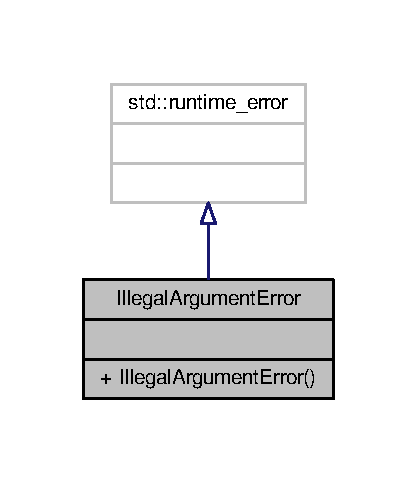
\includegraphics[width=200pt]{classIllegalArgumentError__inherit__graph}
\end{center}
\end{figure}


Collaboration diagram for Illegal\+Argument\+Error\+:\nopagebreak
\begin{figure}[H]
\begin{center}
\leavevmode
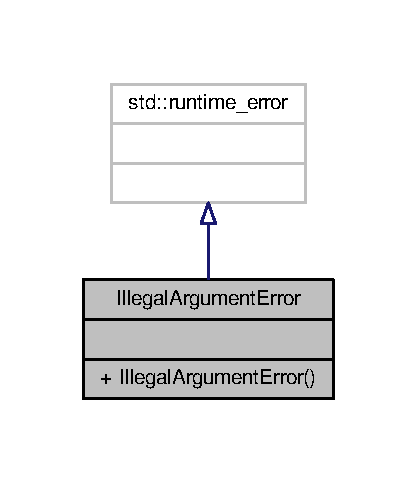
\includegraphics[width=200pt]{classIllegalArgumentError__coll__graph}
\end{center}
\end{figure}
\subsection*{Public Member Functions}
\begin{DoxyCompactItemize}
\item 
\hyperlink{classIllegalArgumentError_aec2c76d99f790765a78e3d4fa109055a}{Illegal\+Argument\+Error} (const char $\ast$msg)
\end{DoxyCompactItemize}


\subsection{Detailed Description}
Error in the parameter of a method. 

\subsection{Constructor \& Destructor Documentation}
\hypertarget{classIllegalArgumentError_aec2c76d99f790765a78e3d4fa109055a}{}\index{Illegal\+Argument\+Error@{Illegal\+Argument\+Error}!Illegal\+Argument\+Error@{Illegal\+Argument\+Error}}
\index{Illegal\+Argument\+Error@{Illegal\+Argument\+Error}!Illegal\+Argument\+Error@{Illegal\+Argument\+Error}}
\subsubsection[{Illegal\+Argument\+Error}]{\setlength{\rightskip}{0pt plus 5cm}Illegal\+Argument\+Error\+::\+Illegal\+Argument\+Error (
\begin{DoxyParamCaption}
\item[{const char $\ast$}]{msg}
\end{DoxyParamCaption}
)\hspace{0.3cm}{\ttfamily [inline]}, {\ttfamily [explicit]}}\label{classIllegalArgumentError_aec2c76d99f790765a78e3d4fa109055a}


The documentation for this class was generated from the following file\+:\begin{DoxyCompactItemize}
\item 
errors/\hyperlink{IllegalArgumentError_8h}{Illegal\+Argument\+Error.\+h}\end{DoxyCompactItemize}

\hypertarget{classIncompatibleTypeError}{}\section{Incompatible\+Type\+Error Class Reference}
\label{classIncompatibleTypeError}\index{Incompatible\+Type\+Error@{Incompatible\+Type\+Error}}


Error in the type of an object.  




{\ttfamily \#include $<$Incompatible\+Type\+Error.\+h$>$}



Inheritance diagram for Incompatible\+Type\+Error\+:\nopagebreak
\begin{figure}[H]
\begin{center}
\leavevmode
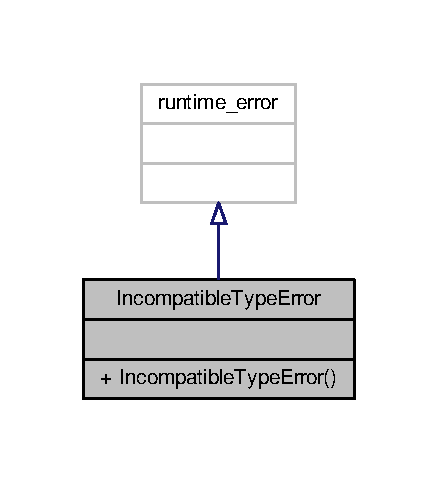
\includegraphics[width=210pt]{classIncompatibleTypeError__inherit__graph}
\end{center}
\end{figure}


Collaboration diagram for Incompatible\+Type\+Error\+:\nopagebreak
\begin{figure}[H]
\begin{center}
\leavevmode
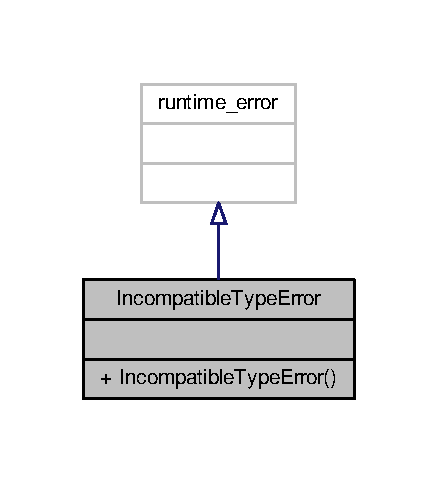
\includegraphics[width=210pt]{classIncompatibleTypeError__coll__graph}
\end{center}
\end{figure}
\subsection*{Public Member Functions}
\begin{DoxyCompactItemize}
\item 
\hyperlink{classIncompatibleTypeError_ab0d9dcc1463ee375b7c0d34d1e5e99d5}{Incompatible\+Type\+Error} (const \hyperlink{CMakeCache_8txt_afe71f11dacb15682cdc012f7208e6e09}{char} $\ast$msg)
\end{DoxyCompactItemize}


\subsection{Detailed Description}
Error in the type of an object. 

\subsection{Constructor \& Destructor Documentation}
\index{Incompatible\+Type\+Error@{Incompatible\+Type\+Error}!Incompatible\+Type\+Error@{Incompatible\+Type\+Error}}
\index{Incompatible\+Type\+Error@{Incompatible\+Type\+Error}!Incompatible\+Type\+Error@{Incompatible\+Type\+Error}}
\subsubsection[{\texorpdfstring{Incompatible\+Type\+Error(const char $\ast$msg)}{IncompatibleTypeError(const char *msg)}}]{\setlength{\rightskip}{0pt plus 5cm}Incompatible\+Type\+Error\+::\+Incompatible\+Type\+Error (
\begin{DoxyParamCaption}
\item[{const {\bf char} $\ast$}]{msg}
\end{DoxyParamCaption}
)\hspace{0.3cm}{\ttfamily [inline]}, {\ttfamily [explicit]}}\hypertarget{classIncompatibleTypeError_ab0d9dcc1463ee375b7c0d34d1e5e99d5}{}\label{classIncompatibleTypeError_ab0d9dcc1463ee375b7c0d34d1e5e99d5}


The documentation for this class was generated from the following file\+:\begin{DoxyCompactItemize}
\item 
errors/\hyperlink{IncompatibleTypeError_8h}{Incompatible\+Type\+Error.\+h}\end{DoxyCompactItemize}

\hypertarget{classInvalidBBAError}{}\section{Invalid\+B\+B\+A\+Error Class Reference}
\label{classInvalidBBAError}\index{Invalid\+B\+B\+A\+Error@{Invalid\+B\+B\+A\+Error}}


Error in the validity of the B\+B\+A of the \hyperlink{classEvidence}{Evidence} object in use.  




{\ttfamily \#include $<$Invalid\+B\+B\+A\+Error.\+h$>$}



Inheritance diagram for Invalid\+B\+B\+A\+Error\+:\nopagebreak
\begin{figure}[H]
\begin{center}
\leavevmode
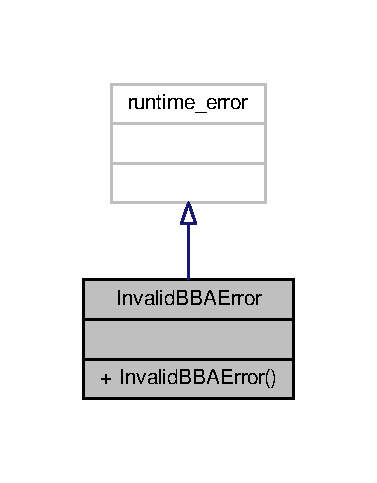
\includegraphics[width=181pt]{classInvalidBBAError__inherit__graph}
\end{center}
\end{figure}


Collaboration diagram for Invalid\+B\+B\+A\+Error\+:\nopagebreak
\begin{figure}[H]
\begin{center}
\leavevmode
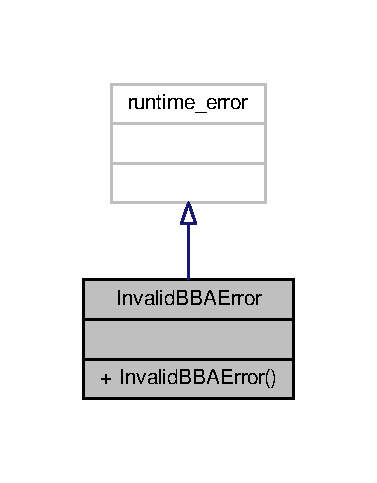
\includegraphics[width=181pt]{classInvalidBBAError__coll__graph}
\end{center}
\end{figure}
\subsection*{Public Member Functions}
\begin{DoxyCompactItemize}
\item 
\hyperlink{classInvalidBBAError_a9c15acd507289023bad4e4079a2c53c6}{Invalid\+B\+B\+A\+Error} (const char $\ast$msg)
\end{DoxyCompactItemize}


\subsection{Detailed Description}
Error in the validity of the B\+B\+A of the \hyperlink{classEvidence}{Evidence} object in use. 

\subsection{Constructor \& Destructor Documentation}
\hypertarget{classInvalidBBAError_a9c15acd507289023bad4e4079a2c53c6}{}\index{Invalid\+B\+B\+A\+Error@{Invalid\+B\+B\+A\+Error}!Invalid\+B\+B\+A\+Error@{Invalid\+B\+B\+A\+Error}}
\index{Invalid\+B\+B\+A\+Error@{Invalid\+B\+B\+A\+Error}!Invalid\+B\+B\+A\+Error@{Invalid\+B\+B\+A\+Error}}
\subsubsection[{Invalid\+B\+B\+A\+Error}]{\setlength{\rightskip}{0pt plus 5cm}Invalid\+B\+B\+A\+Error\+::\+Invalid\+B\+B\+A\+Error (
\begin{DoxyParamCaption}
\item[{const char $\ast$}]{msg}
\end{DoxyParamCaption}
)\hspace{0.3cm}{\ttfamily [inline]}, {\ttfamily [explicit]}}\label{classInvalidBBAError_a9c15acd507289023bad4e4079a2c53c6}


The documentation for this class was generated from the following file\+:\begin{DoxyCompactItemize}
\item 
errors/\hyperlink{InvalidBBAError_8h}{Invalid\+B\+B\+A\+Error.\+h}\end{DoxyCompactItemize}

\hypertarget{classGeometry_1_1Point2D}{}\section{Geometry\+:\+:Point2D Class Reference}
\label{classGeometry_1_1Point2D}\index{Geometry\+::\+Point2D@{Geometry\+::\+Point2D}}


2D point in integer coordinates.  




{\ttfamily \#include $<$Point2\+D.\+h$>$}



Collaboration diagram for Geometry\+:\+:Point2D\+:\nopagebreak
\begin{figure}[H]
\begin{center}
\leavevmode
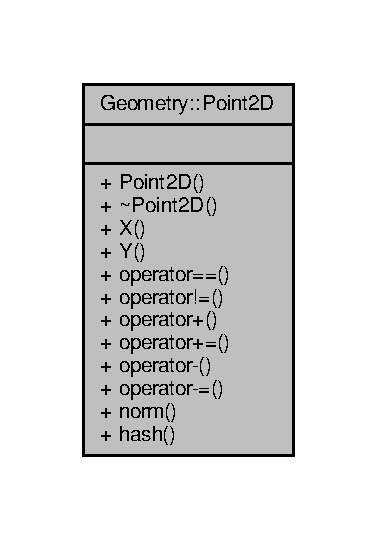
\includegraphics[width=181pt]{classGeometry_1_1Point2D__coll__graph}
\end{center}
\end{figure}
\subsection*{Public Member Functions}
\begin{DoxyCompactItemize}
\item 
\hyperlink{classGeometry_1_1Point2D_a873dc5d6e2f707d70b74e88265a595f6}{Point2D} (long x=0, long y=0)
\begin{DoxyCompactList}\small\item\em Construcor. \end{DoxyCompactList}\item 
virtual \hyperlink{classGeometry_1_1Point2D_a2347379e70ce2907fc497557217e10a3}{$\sim$\+Point2D} ()=default
\item 
long \hyperlink{classGeometry_1_1Point2D_adba56a7597877f2857f019b619c1b31c}{X} () const 
\begin{DoxyCompactList}\small\item\em Get x. \end{DoxyCompactList}\item 
long \hyperlink{classGeometry_1_1Point2D_a766b1824c060c5e625903e6910842f46}{Y} () const 
\begin{DoxyCompactList}\small\item\em Get y. \end{DoxyCompactList}\item 
bool \hyperlink{classGeometry_1_1Point2D_a7ce87ad250d9a716df2d293f8af2accf}{operator==} (const \hyperlink{classGeometry_1_1Point2D}{Point2D} \&rhs) const 
\item 
bool \hyperlink{classGeometry_1_1Point2D_ad97232d7ab2ef71fd78c80796b1654b8}{operator!=} (const \hyperlink{classGeometry_1_1Point2D}{Point2D} \&rhs) const 
\item 
\hyperlink{classGeometry_1_1Point2D}{Point2D} \hyperlink{classGeometry_1_1Point2D_a6c759799b1a736881db4bfe7cbed3ece}{operator+} (const \hyperlink{classGeometry_1_1Point2D}{Point2D} \&rhs) const 
\item 
\hyperlink{classGeometry_1_1Point2D}{Point2D} \& \hyperlink{classGeometry_1_1Point2D_afae0ca03e239fbfbbca63ab76ffdc048}{operator+=} (const \hyperlink{classGeometry_1_1Point2D}{Point2D} \&rhs)
\item 
\hyperlink{classGeometry_1_1Point2D}{Point2D} \hyperlink{classGeometry_1_1Point2D_afb1f91842fd1d67fc404570512ccb03f}{operator-\/} (const \hyperlink{classGeometry_1_1Point2D}{Point2D} \&rhs) const 
\item 
\hyperlink{classGeometry_1_1Point2D}{Point2D} \& \hyperlink{classGeometry_1_1Point2D_aa1993e7157ec63caf7ec10217daafdaf}{operator-\/=} (const \hyperlink{classGeometry_1_1Point2D}{Point2D} \&rhs)
\item 
double \hyperlink{classGeometry_1_1Point2D_a27ecff835c81977e9c2dfcabe34a0e29}{norm} () const 
\item 
size\+\_\+t \hyperlink{classGeometry_1_1Point2D_a45a03b466fadbd77c00480017278519b}{hash} () const 
\end{DoxyCompactItemize}
\subsection*{Friends}
\begin{DoxyCompactItemize}
\item 
std\+::ostream \& \hyperlink{classGeometry_1_1Point2D_a2ec03e8e9f734d37ee69c16cb02d69de}{operator$<$$<$} (std\+::ostream \&os, const \hyperlink{classGeometry_1_1Point2D}{Point2D} \&d)
\end{DoxyCompactItemize}


\subsection{Detailed Description}
2D point in integer coordinates. 

\subsection{Constructor \& Destructor Documentation}
\index{Geometry\+::\+Point2D@{Geometry\+::\+Point2D}!Point2D@{Point2D}}
\index{Point2D@{Point2D}!Geometry\+::\+Point2D@{Geometry\+::\+Point2D}}
\subsubsection[{\texorpdfstring{Point2\+D(long x=0, long y=0)}{Point2D(long x=0, long y=0)}}]{\setlength{\rightskip}{0pt plus 5cm}Geometry\+::\+Point2\+D\+::\+Point2D (
\begin{DoxyParamCaption}
\item[{long}]{x = {\ttfamily 0}, }
\item[{long}]{y = {\ttfamily 0}}
\end{DoxyParamCaption}
)\hspace{0.3cm}{\ttfamily [inline]}, {\ttfamily [explicit]}}\hypertarget{classGeometry_1_1Point2D_a873dc5d6e2f707d70b74e88265a595f6}{}\label{classGeometry_1_1Point2D_a873dc5d6e2f707d70b74e88265a595f6}


Construcor. 


\begin{DoxyParams}{Parameters}
{\em x} & \\
\hline
{\em y} & \\
\hline
\end{DoxyParams}
\index{Geometry\+::\+Point2D@{Geometry\+::\+Point2D}!````~Point2D@{$\sim$\+Point2D}}
\index{````~Point2D@{$\sim$\+Point2D}!Geometry\+::\+Point2D@{Geometry\+::\+Point2D}}
\subsubsection[{\texorpdfstring{$\sim$\+Point2\+D()=default}{~Point2D()=default}}]{\setlength{\rightskip}{0pt plus 5cm}virtual Geometry\+::\+Point2\+D\+::$\sim$\+Point2D (
\begin{DoxyParamCaption}
{}
\end{DoxyParamCaption}
)\hspace{0.3cm}{\ttfamily [virtual]}, {\ttfamily [default]}}\hypertarget{classGeometry_1_1Point2D_a2347379e70ce2907fc497557217e10a3}{}\label{classGeometry_1_1Point2D_a2347379e70ce2907fc497557217e10a3}


\subsection{Member Function Documentation}
\index{Geometry\+::\+Point2D@{Geometry\+::\+Point2D}!hash@{hash}}
\index{hash@{hash}!Geometry\+::\+Point2D@{Geometry\+::\+Point2D}}
\subsubsection[{\texorpdfstring{hash() const }{hash() const }}]{\setlength{\rightskip}{0pt plus 5cm}size\+\_\+t Geometry\+::\+Point2\+D\+::hash (
\begin{DoxyParamCaption}
{}
\end{DoxyParamCaption}
) const\hspace{0.3cm}{\ttfamily [inline]}}\hypertarget{classGeometry_1_1Point2D_a45a03b466fadbd77c00480017278519b}{}\label{classGeometry_1_1Point2D_a45a03b466fadbd77c00480017278519b}
\index{Geometry\+::\+Point2D@{Geometry\+::\+Point2D}!norm@{norm}}
\index{norm@{norm}!Geometry\+::\+Point2D@{Geometry\+::\+Point2D}}
\subsubsection[{\texorpdfstring{norm() const }{norm() const }}]{\setlength{\rightskip}{0pt plus 5cm}double Geometry\+::\+Point2\+D\+::norm (
\begin{DoxyParamCaption}
{}
\end{DoxyParamCaption}
) const\hspace{0.3cm}{\ttfamily [inline]}}\hypertarget{classGeometry_1_1Point2D_a27ecff835c81977e9c2dfcabe34a0e29}{}\label{classGeometry_1_1Point2D_a27ecff835c81977e9c2dfcabe34a0e29}
\index{Geometry\+::\+Point2D@{Geometry\+::\+Point2D}!operator"!=@{operator"!=}}
\index{operator"!=@{operator"!=}!Geometry\+::\+Point2D@{Geometry\+::\+Point2D}}
\subsubsection[{\texorpdfstring{operator"!=(const Point2\+D \&rhs) const }{operator!=(const Point2D &rhs) const }}]{\setlength{\rightskip}{0pt plus 5cm}bool Geometry\+::\+Point2\+D\+::operator!= (
\begin{DoxyParamCaption}
\item[{const {\bf Point2D} \&}]{rhs}
\end{DoxyParamCaption}
) const\hspace{0.3cm}{\ttfamily [inline]}}\hypertarget{classGeometry_1_1Point2D_ad97232d7ab2ef71fd78c80796b1654b8}{}\label{classGeometry_1_1Point2D_ad97232d7ab2ef71fd78c80796b1654b8}
\index{Geometry\+::\+Point2D@{Geometry\+::\+Point2D}!operator+@{operator+}}
\index{operator+@{operator+}!Geometry\+::\+Point2D@{Geometry\+::\+Point2D}}
\subsubsection[{\texorpdfstring{operator+(const Point2\+D \&rhs) const }{operator+(const Point2D &rhs) const }}]{\setlength{\rightskip}{0pt plus 5cm}{\bf Point2D} Geometry\+::\+Point2\+D\+::operator+ (
\begin{DoxyParamCaption}
\item[{const {\bf Point2D} \&}]{rhs}
\end{DoxyParamCaption}
) const\hspace{0.3cm}{\ttfamily [inline]}}\hypertarget{classGeometry_1_1Point2D_a6c759799b1a736881db4bfe7cbed3ece}{}\label{classGeometry_1_1Point2D_a6c759799b1a736881db4bfe7cbed3ece}
\index{Geometry\+::\+Point2D@{Geometry\+::\+Point2D}!operator+=@{operator+=}}
\index{operator+=@{operator+=}!Geometry\+::\+Point2D@{Geometry\+::\+Point2D}}
\subsubsection[{\texorpdfstring{operator+=(const Point2\+D \&rhs)}{operator+=(const Point2D &rhs)}}]{\setlength{\rightskip}{0pt plus 5cm}{\bf Point2D}\& Geometry\+::\+Point2\+D\+::operator+= (
\begin{DoxyParamCaption}
\item[{const {\bf Point2D} \&}]{rhs}
\end{DoxyParamCaption}
)\hspace{0.3cm}{\ttfamily [inline]}}\hypertarget{classGeometry_1_1Point2D_afae0ca03e239fbfbbca63ab76ffdc048}{}\label{classGeometry_1_1Point2D_afae0ca03e239fbfbbca63ab76ffdc048}
\index{Geometry\+::\+Point2D@{Geometry\+::\+Point2D}!operator-\/@{operator-\/}}
\index{operator-\/@{operator-\/}!Geometry\+::\+Point2D@{Geometry\+::\+Point2D}}
\subsubsection[{\texorpdfstring{operator-\/(const Point2\+D \&rhs) const }{operator-(const Point2D &rhs) const }}]{\setlength{\rightskip}{0pt plus 5cm}{\bf Point2D} Geometry\+::\+Point2\+D\+::operator-\/ (
\begin{DoxyParamCaption}
\item[{const {\bf Point2D} \&}]{rhs}
\end{DoxyParamCaption}
) const\hspace{0.3cm}{\ttfamily [inline]}}\hypertarget{classGeometry_1_1Point2D_afb1f91842fd1d67fc404570512ccb03f}{}\label{classGeometry_1_1Point2D_afb1f91842fd1d67fc404570512ccb03f}
\index{Geometry\+::\+Point2D@{Geometry\+::\+Point2D}!operator-\/=@{operator-\/=}}
\index{operator-\/=@{operator-\/=}!Geometry\+::\+Point2D@{Geometry\+::\+Point2D}}
\subsubsection[{\texorpdfstring{operator-\/=(const Point2\+D \&rhs)}{operator-=(const Point2D &rhs)}}]{\setlength{\rightskip}{0pt plus 5cm}{\bf Point2D}\& Geometry\+::\+Point2\+D\+::operator-\/= (
\begin{DoxyParamCaption}
\item[{const {\bf Point2D} \&}]{rhs}
\end{DoxyParamCaption}
)\hspace{0.3cm}{\ttfamily [inline]}}\hypertarget{classGeometry_1_1Point2D_aa1993e7157ec63caf7ec10217daafdaf}{}\label{classGeometry_1_1Point2D_aa1993e7157ec63caf7ec10217daafdaf}
\index{Geometry\+::\+Point2D@{Geometry\+::\+Point2D}!operator==@{operator==}}
\index{operator==@{operator==}!Geometry\+::\+Point2D@{Geometry\+::\+Point2D}}
\subsubsection[{\texorpdfstring{operator==(const Point2\+D \&rhs) const }{operator==(const Point2D &rhs) const }}]{\setlength{\rightskip}{0pt plus 5cm}bool Geometry\+::\+Point2\+D\+::operator== (
\begin{DoxyParamCaption}
\item[{const {\bf Point2D} \&}]{rhs}
\end{DoxyParamCaption}
) const\hspace{0.3cm}{\ttfamily [inline]}}\hypertarget{classGeometry_1_1Point2D_a7ce87ad250d9a716df2d293f8af2accf}{}\label{classGeometry_1_1Point2D_a7ce87ad250d9a716df2d293f8af2accf}
\index{Geometry\+::\+Point2D@{Geometry\+::\+Point2D}!X@{X}}
\index{X@{X}!Geometry\+::\+Point2D@{Geometry\+::\+Point2D}}
\subsubsection[{\texorpdfstring{X() const }{X() const }}]{\setlength{\rightskip}{0pt plus 5cm}long Geometry\+::\+Point2\+D\+::X (
\begin{DoxyParamCaption}
{}
\end{DoxyParamCaption}
) const\hspace{0.3cm}{\ttfamily [inline]}}\hypertarget{classGeometry_1_1Point2D_adba56a7597877f2857f019b619c1b31c}{}\label{classGeometry_1_1Point2D_adba56a7597877f2857f019b619c1b31c}


Get x. 

\begin{DoxyReturn}{Returns}
x. 
\end{DoxyReturn}
\index{Geometry\+::\+Point2D@{Geometry\+::\+Point2D}!Y@{Y}}
\index{Y@{Y}!Geometry\+::\+Point2D@{Geometry\+::\+Point2D}}
\subsubsection[{\texorpdfstring{Y() const }{Y() const }}]{\setlength{\rightskip}{0pt plus 5cm}long Geometry\+::\+Point2\+D\+::Y (
\begin{DoxyParamCaption}
{}
\end{DoxyParamCaption}
) const\hspace{0.3cm}{\ttfamily [inline]}}\hypertarget{classGeometry_1_1Point2D_a766b1824c060c5e625903e6910842f46}{}\label{classGeometry_1_1Point2D_a766b1824c060c5e625903e6910842f46}


Get y. 

\begin{DoxyReturn}{Returns}
y. 
\end{DoxyReturn}


\subsection{Friends And Related Function Documentation}
\index{Geometry\+::\+Point2D@{Geometry\+::\+Point2D}!operator$<$$<$@{operator$<$$<$}}
\index{operator$<$$<$@{operator$<$$<$}!Geometry\+::\+Point2D@{Geometry\+::\+Point2D}}
\subsubsection[{\texorpdfstring{operator$<$$<$}{operator<<}}]{\setlength{\rightskip}{0pt plus 5cm}std\+::ostream\& operator$<$$<$ (
\begin{DoxyParamCaption}
\item[{std\+::ostream \&}]{os, }
\item[{const {\bf Point2D} \&}]{d}
\end{DoxyParamCaption}
)\hspace{0.3cm}{\ttfamily [friend]}}\hypertarget{classGeometry_1_1Point2D_a2ec03e8e9f734d37ee69c16cb02d69de}{}\label{classGeometry_1_1Point2D_a2ec03e8e9f734d37ee69c16cb02d69de}


The documentation for this class was generated from the following file\+:\begin{DoxyCompactItemize}
\item 
geometry/\hyperlink{Point2D_8h}{Point2\+D.\+h}\end{DoxyCompactItemize}

\hypertarget{classGeometry_1_1Rectangle}{}\section{Geometry\+:\+:Rectangle Class Reference}
\label{classGeometry_1_1Rectangle}\index{Geometry\+::\+Rectangle@{Geometry\+::\+Rectangle}}


\hyperlink{classGeometry_1_1Rectangle}{Rectangle} parallel to the plane axis.  




{\ttfamily \#include $<$Rectangle.\+h$>$}



Inheritance diagram for Geometry\+:\+:Rectangle\+:\nopagebreak
\begin{figure}[H]
\begin{center}
\leavevmode
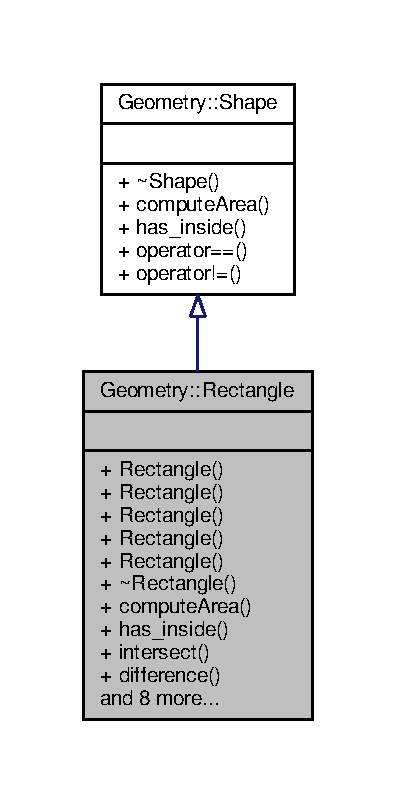
\includegraphics[width=190pt]{classGeometry_1_1Rectangle__inherit__graph}
\end{center}
\end{figure}


Collaboration diagram for Geometry\+:\+:Rectangle\+:\nopagebreak
\begin{figure}[H]
\begin{center}
\leavevmode
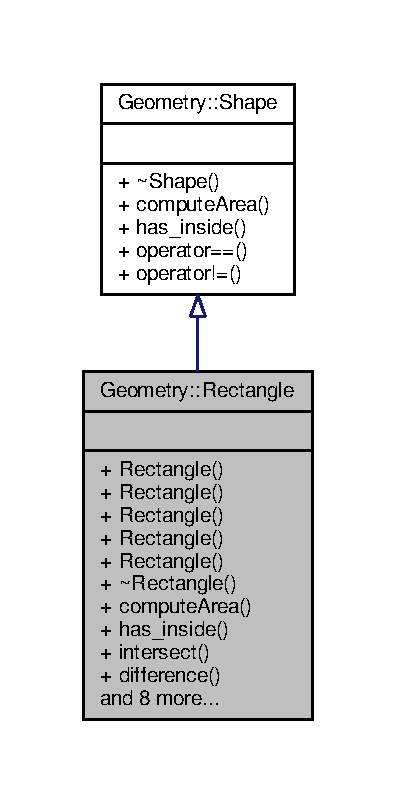
\includegraphics[width=190pt]{classGeometry_1_1Rectangle__coll__graph}
\end{center}
\end{figure}
\subsection*{Public Member Functions}
\begin{DoxyCompactItemize}
\item 
\hyperlink{classGeometry_1_1Rectangle_a3a73665b3e36e9d73968ca77eece4552}{Rectangle} ()
\item 
\hyperlink{classGeometry_1_1Rectangle_a6e9d73d75bafe76243b6939f0630897c}{Rectangle} (long xmin, long xmax, long ymin, long ymax)
\begin{DoxyCompactList}\small\item\em Constructor. \end{DoxyCompactList}\item 
\hyperlink{classGeometry_1_1Rectangle_af43cb3bd05884b9edd3cadfacbf379f7}{Rectangle} (std\+::vector$<$ \hyperlink{classGeometry_1_1Point2D}{Point2D} $>$ \&vertices)
\begin{DoxyCompactList}\small\item\em Constructor. \end{DoxyCompactList}\item 
\hyperlink{classGeometry_1_1Rectangle_a03200e2f3bb2e4fca3b2f76d768e5c95}{Rectangle} (\hyperlink{classGeometry_1_1Point2D}{Point2D} p1, \hyperlink{classGeometry_1_1Point2D}{Point2D} p2)
\begin{DoxyCompactList}\small\item\em Constructor. \end{DoxyCompactList}\item 
\hyperlink{classGeometry_1_1Rectangle_ae609ed3d87f6dc59d5a0aae1c17709aa}{Rectangle} (\hyperlink{classGeometry_1_1Point2D}{Point2D} p\+\_\+up\+\_\+left, long width, long height)
\begin{DoxyCompactList}\small\item\em Constructor. \end{DoxyCompactList}\item 
\hyperlink{classGeometry_1_1Rectangle_a29f446cb310ac71f9826ee9c8226191b}{$\sim$\+Rectangle} () override=default
\item 
double \hyperlink{classGeometry_1_1Rectangle_adcae3b63e18582f1d4983dfa80029fb7}{compute\+Area} () const override
\begin{DoxyCompactList}\small\item\em Get the area of the shape. \end{DoxyCompactList}\item 
bool \hyperlink{classGeometry_1_1Rectangle_ab186008b8f7c4b99fec564021c40e3eb}{has\+\_\+inside} (\hyperlink{classGeometry_1_1Point2D}{Point2D} p) const override
\begin{DoxyCompactList}\small\item\em Check if the point is inside the current shape. \end{DoxyCompactList}\item 
\hyperlink{classGeometry_1_1Rectangle}{Rectangle} \hyperlink{classGeometry_1_1Rectangle_afd899e69807bf618719805dff42f574d}{intersect} (const \hyperlink{classGeometry_1_1Rectangle}{Rectangle} \&other) const 
\begin{DoxyCompactList}\small\item\em Intersect a \hyperlink{classGeometry_1_1Rectangle}{Rectangle} with another one. \end{DoxyCompactList}\item 
std\+::vector$<$ \hyperlink{classGeometry_1_1Rectangle}{Rectangle} $>$ \hyperlink{classGeometry_1_1Rectangle_ac803730dcde1c4e059abd1dc962b6314}{difference} (const \hyperlink{classGeometry_1_1Rectangle}{Rectangle} \&other) const 
\begin{DoxyCompactList}\small\item\em Apply difference operator with another \hyperlink{classGeometry_1_1Rectangle}{Rectangle}. \end{DoxyCompactList}\item 
long \hyperlink{classGeometry_1_1Rectangle_a8deb4fa571eaa05911456c14e2fa25ab}{get\+Xmin} () const 
\begin{DoxyCompactList}\small\item\em Get xmin. \end{DoxyCompactList}\item 
long \hyperlink{classGeometry_1_1Rectangle_ab034b771c6a3d7c482daac66a0d97ad8}{get\+Xmax} () const 
\begin{DoxyCompactList}\small\item\em Get xmax. \end{DoxyCompactList}\item 
long \hyperlink{classGeometry_1_1Rectangle_a4fd564dbf894c57e3b04c5f1d9f139cd}{get\+Ymin} () const 
\begin{DoxyCompactList}\small\item\em Get ymin. \end{DoxyCompactList}\item 
long \hyperlink{classGeometry_1_1Rectangle_aebea5b9d1990639bac462fa00714d4a1}{get\+Ymax} () const 
\begin{DoxyCompactList}\small\item\em Get ymax. \end{DoxyCompactList}\item 
void \hyperlink{classGeometry_1_1Rectangle_a9429d96831fcf302b35306187a1a5c87}{set\+Xmin} (long xmin)
\begin{DoxyCompactList}\small\item\em Set xmin. \end{DoxyCompactList}\item 
void \hyperlink{classGeometry_1_1Rectangle_af4a0d6ea20241c23ace59d198fd5de3c}{set\+Xmax} (long xmax)
\begin{DoxyCompactList}\small\item\em Set xmax. \end{DoxyCompactList}\item 
void \hyperlink{classGeometry_1_1Rectangle_a9cd50d8752fbf874d9979cf7189963f4}{set\+Ymin} (long ymin)
\begin{DoxyCompactList}\small\item\em Set ymin. \end{DoxyCompactList}\item 
void \hyperlink{classGeometry_1_1Rectangle_abc92fe5c878653505e409686aeb614f8}{set\+Ymax} (long ymax)
\begin{DoxyCompactList}\small\item\em Set ymax. \end{DoxyCompactList}\end{DoxyCompactItemize}
\subsection*{Friends}
\begin{DoxyCompactItemize}
\item 
std\+::ostream \& \hyperlink{classGeometry_1_1Rectangle_a6928c586de0f57714ed6e389186c94c2}{operator$<$$<$} (std\+::ostream \&os, const \hyperlink{classGeometry_1_1Rectangle}{Rectangle} \&rectangle)
\end{DoxyCompactItemize}


\subsection{Detailed Description}
\hyperlink{classGeometry_1_1Rectangle}{Rectangle} parallel to the plane axis. 

\subsection{Constructor \& Destructor Documentation}
\index{Geometry\+::\+Rectangle@{Geometry\+::\+Rectangle}!Rectangle@{Rectangle}}
\index{Rectangle@{Rectangle}!Geometry\+::\+Rectangle@{Geometry\+::\+Rectangle}}
\subsubsection[{\texorpdfstring{Rectangle()}{Rectangle()}}]{\setlength{\rightskip}{0pt plus 5cm}Geometry\+::\+Rectangle\+::\+Rectangle (
\begin{DoxyParamCaption}
{}
\end{DoxyParamCaption}
)\hspace{0.3cm}{\ttfamily [inline]}}\hypertarget{classGeometry_1_1Rectangle_a3a73665b3e36e9d73968ca77eece4552}{}\label{classGeometry_1_1Rectangle_a3a73665b3e36e9d73968ca77eece4552}
\index{Geometry\+::\+Rectangle@{Geometry\+::\+Rectangle}!Rectangle@{Rectangle}}
\index{Rectangle@{Rectangle}!Geometry\+::\+Rectangle@{Geometry\+::\+Rectangle}}
\subsubsection[{\texorpdfstring{Rectangle(long xmin, long xmax, long ymin, long ymax)}{Rectangle(long xmin, long xmax, long ymin, long ymax)}}]{\setlength{\rightskip}{0pt plus 5cm}Geometry\+::\+Rectangle\+::\+Rectangle (
\begin{DoxyParamCaption}
\item[{long}]{xmin, }
\item[{long}]{xmax, }
\item[{long}]{ymin, }
\item[{long}]{ymax}
\end{DoxyParamCaption}
)\hspace{0.3cm}{\ttfamily [inline]}}\hypertarget{classGeometry_1_1Rectangle_a6e9d73d75bafe76243b6939f0630897c}{}\label{classGeometry_1_1Rectangle_a6e9d73d75bafe76243b6939f0630897c}


Constructor. 


\begin{DoxyParams}{Parameters}
{\em xmin} & \\
\hline
{\em xmax} & \\
\hline
{\em ymin} & \\
\hline
{\em ymax} & \\
\hline
\end{DoxyParams}
\index{Geometry\+::\+Rectangle@{Geometry\+::\+Rectangle}!Rectangle@{Rectangle}}
\index{Rectangle@{Rectangle}!Geometry\+::\+Rectangle@{Geometry\+::\+Rectangle}}
\subsubsection[{\texorpdfstring{Rectangle(std\+::vector$<$ Point2\+D $>$ \&vertices)}{Rectangle(std::vector< Point2D > &vertices)}}]{\setlength{\rightskip}{0pt plus 5cm}Geometry\+::\+Rectangle\+::\+Rectangle (
\begin{DoxyParamCaption}
\item[{std\+::vector$<$ {\bf Point2D} $>$ \&}]{vertices}
\end{DoxyParamCaption}
)\hspace{0.3cm}{\ttfamily [explicit]}}\hypertarget{classGeometry_1_1Rectangle_af43cb3bd05884b9edd3cadfacbf379f7}{}\label{classGeometry_1_1Rectangle_af43cb3bd05884b9edd3cadfacbf379f7}


Constructor. 


\begin{DoxyParams}{Parameters}
{\em vertices} & Array of vertices. \\
\hline
\end{DoxyParams}
\index{Geometry\+::\+Rectangle@{Geometry\+::\+Rectangle}!Rectangle@{Rectangle}}
\index{Rectangle@{Rectangle}!Geometry\+::\+Rectangle@{Geometry\+::\+Rectangle}}
\subsubsection[{\texorpdfstring{Rectangle(\+Point2\+D p1, Point2\+D p2)}{Rectangle(Point2D p1, Point2D p2)}}]{\setlength{\rightskip}{0pt plus 5cm}Geometry\+::\+Rectangle\+::\+Rectangle (
\begin{DoxyParamCaption}
\item[{{\bf Point2D}}]{p1, }
\item[{{\bf Point2D}}]{p2}
\end{DoxyParamCaption}
)}\hypertarget{classGeometry_1_1Rectangle_a03200e2f3bb2e4fca3b2f76d768e5c95}{}\label{classGeometry_1_1Rectangle_a03200e2f3bb2e4fca3b2f76d768e5c95}


Constructor. 


\begin{DoxyParams}{Parameters}
{\em p1} & top-\/left corner \\
\hline
{\em p2} & bottom-\/right corner \\
\hline
\end{DoxyParams}
\index{Geometry\+::\+Rectangle@{Geometry\+::\+Rectangle}!Rectangle@{Rectangle}}
\index{Rectangle@{Rectangle}!Geometry\+::\+Rectangle@{Geometry\+::\+Rectangle}}
\subsubsection[{\texorpdfstring{Rectangle(\+Point2\+D p\+\_\+up\+\_\+left, long width, long height)}{Rectangle(Point2D p_up_left, long width, long height)}}]{\setlength{\rightskip}{0pt plus 5cm}Geometry\+::\+Rectangle\+::\+Rectangle (
\begin{DoxyParamCaption}
\item[{{\bf Point2D}}]{p\+\_\+up\+\_\+left, }
\item[{long}]{width, }
\item[{long}]{height}
\end{DoxyParamCaption}
)}\hypertarget{classGeometry_1_1Rectangle_ae609ed3d87f6dc59d5a0aae1c17709aa}{}\label{classGeometry_1_1Rectangle_ae609ed3d87f6dc59d5a0aae1c17709aa}


Constructor. 


\begin{DoxyParams}{Parameters}
{\em p\+\_\+up\+\_\+left} & to-\/left corner \\
\hline
{\em width} & \\
\hline
{\em height} & \\
\hline
\end{DoxyParams}
\index{Geometry\+::\+Rectangle@{Geometry\+::\+Rectangle}!````~Rectangle@{$\sim$\+Rectangle}}
\index{````~Rectangle@{$\sim$\+Rectangle}!Geometry\+::\+Rectangle@{Geometry\+::\+Rectangle}}
\subsubsection[{\texorpdfstring{$\sim$\+Rectangle() override=default}{~Rectangle() override=default}}]{\setlength{\rightskip}{0pt plus 5cm}Geometry\+::\+Rectangle\+::$\sim$\+Rectangle (
\begin{DoxyParamCaption}
{}
\end{DoxyParamCaption}
)\hspace{0.3cm}{\ttfamily [override]}, {\ttfamily [default]}}\hypertarget{classGeometry_1_1Rectangle_a29f446cb310ac71f9826ee9c8226191b}{}\label{classGeometry_1_1Rectangle_a29f446cb310ac71f9826ee9c8226191b}


\subsection{Member Function Documentation}
\index{Geometry\+::\+Rectangle@{Geometry\+::\+Rectangle}!compute\+Area@{compute\+Area}}
\index{compute\+Area@{compute\+Area}!Geometry\+::\+Rectangle@{Geometry\+::\+Rectangle}}
\subsubsection[{\texorpdfstring{compute\+Area() const override}{computeArea() const override}}]{\setlength{\rightskip}{0pt plus 5cm}double Geometry\+::\+Rectangle\+::compute\+Area (
\begin{DoxyParamCaption}
{}
\end{DoxyParamCaption}
) const\hspace{0.3cm}{\ttfamily [override]}, {\ttfamily [virtual]}}\hypertarget{classGeometry_1_1Rectangle_adcae3b63e18582f1d4983dfa80029fb7}{}\label{classGeometry_1_1Rectangle_adcae3b63e18582f1d4983dfa80029fb7}


Get the area of the shape. 

\begin{DoxyReturn}{Returns}
Area. 
\end{DoxyReturn}


Implements \hyperlink{classGeometry_1_1Shape_ad0fb97e79dc8c171482bc14726ad8ce7}{Geometry\+::\+Shape}.

\index{Geometry\+::\+Rectangle@{Geometry\+::\+Rectangle}!difference@{difference}}
\index{difference@{difference}!Geometry\+::\+Rectangle@{Geometry\+::\+Rectangle}}
\subsubsection[{\texorpdfstring{difference(const Rectangle \&other) const }{difference(const Rectangle &other) const }}]{\setlength{\rightskip}{0pt plus 5cm}std\+::vector$<$ {\bf Rectangle} $>$ Geometry\+::\+Rectangle\+::difference (
\begin{DoxyParamCaption}
\item[{const {\bf Rectangle} \&}]{other}
\end{DoxyParamCaption}
) const}\hypertarget{classGeometry_1_1Rectangle_ac803730dcde1c4e059abd1dc962b6314}{}\label{classGeometry_1_1Rectangle_ac803730dcde1c4e059abd1dc962b6314}


Apply difference operator with another \hyperlink{classGeometry_1_1Rectangle}{Rectangle}. 


\begin{DoxyParams}{Parameters}
{\em other} & The other \hyperlink{classGeometry_1_1Rectangle}{Rectangle} \\
\hline
\end{DoxyParams}
\begin{DoxyReturn}{Returns}
Array of Rectangles of size from 0 to 4. 
\end{DoxyReturn}
\index{Geometry\+::\+Rectangle@{Geometry\+::\+Rectangle}!get\+Xmax@{get\+Xmax}}
\index{get\+Xmax@{get\+Xmax}!Geometry\+::\+Rectangle@{Geometry\+::\+Rectangle}}
\subsubsection[{\texorpdfstring{get\+Xmax() const }{getXmax() const }}]{\setlength{\rightskip}{0pt plus 5cm}long Geometry\+::\+Rectangle\+::get\+Xmax (
\begin{DoxyParamCaption}
{}
\end{DoxyParamCaption}
) const}\hypertarget{classGeometry_1_1Rectangle_ab034b771c6a3d7c482daac66a0d97ad8}{}\label{classGeometry_1_1Rectangle_ab034b771c6a3d7c482daac66a0d97ad8}


Get xmax. 

\begin{DoxyReturn}{Returns}
xmax 
\end{DoxyReturn}
\index{Geometry\+::\+Rectangle@{Geometry\+::\+Rectangle}!get\+Xmin@{get\+Xmin}}
\index{get\+Xmin@{get\+Xmin}!Geometry\+::\+Rectangle@{Geometry\+::\+Rectangle}}
\subsubsection[{\texorpdfstring{get\+Xmin() const }{getXmin() const }}]{\setlength{\rightskip}{0pt plus 5cm}long Geometry\+::\+Rectangle\+::get\+Xmin (
\begin{DoxyParamCaption}
{}
\end{DoxyParamCaption}
) const}\hypertarget{classGeometry_1_1Rectangle_a8deb4fa571eaa05911456c14e2fa25ab}{}\label{classGeometry_1_1Rectangle_a8deb4fa571eaa05911456c14e2fa25ab}


Get xmin. 

\begin{DoxyReturn}{Returns}
xmin 
\end{DoxyReturn}
\index{Geometry\+::\+Rectangle@{Geometry\+::\+Rectangle}!get\+Ymax@{get\+Ymax}}
\index{get\+Ymax@{get\+Ymax}!Geometry\+::\+Rectangle@{Geometry\+::\+Rectangle}}
\subsubsection[{\texorpdfstring{get\+Ymax() const }{getYmax() const }}]{\setlength{\rightskip}{0pt plus 5cm}long Geometry\+::\+Rectangle\+::get\+Ymax (
\begin{DoxyParamCaption}
{}
\end{DoxyParamCaption}
) const}\hypertarget{classGeometry_1_1Rectangle_aebea5b9d1990639bac462fa00714d4a1}{}\label{classGeometry_1_1Rectangle_aebea5b9d1990639bac462fa00714d4a1}


Get ymax. 

\begin{DoxyReturn}{Returns}
ymax 
\end{DoxyReturn}
\index{Geometry\+::\+Rectangle@{Geometry\+::\+Rectangle}!get\+Ymin@{get\+Ymin}}
\index{get\+Ymin@{get\+Ymin}!Geometry\+::\+Rectangle@{Geometry\+::\+Rectangle}}
\subsubsection[{\texorpdfstring{get\+Ymin() const }{getYmin() const }}]{\setlength{\rightskip}{0pt plus 5cm}long Geometry\+::\+Rectangle\+::get\+Ymin (
\begin{DoxyParamCaption}
{}
\end{DoxyParamCaption}
) const}\hypertarget{classGeometry_1_1Rectangle_a4fd564dbf894c57e3b04c5f1d9f139cd}{}\label{classGeometry_1_1Rectangle_a4fd564dbf894c57e3b04c5f1d9f139cd}


Get ymin. 

\begin{DoxyReturn}{Returns}
ymin 
\end{DoxyReturn}
\index{Geometry\+::\+Rectangle@{Geometry\+::\+Rectangle}!has\+\_\+inside@{has\+\_\+inside}}
\index{has\+\_\+inside@{has\+\_\+inside}!Geometry\+::\+Rectangle@{Geometry\+::\+Rectangle}}
\subsubsection[{\texorpdfstring{has\+\_\+inside(\+Point2\+D p) const override}{has_inside(Point2D p) const override}}]{\setlength{\rightskip}{0pt plus 5cm}bool Geometry\+::\+Rectangle\+::has\+\_\+inside (
\begin{DoxyParamCaption}
\item[{{\bf Point2D}}]{p}
\end{DoxyParamCaption}
) const\hspace{0.3cm}{\ttfamily [override]}, {\ttfamily [virtual]}}\hypertarget{classGeometry_1_1Rectangle_ab186008b8f7c4b99fec564021c40e3eb}{}\label{classGeometry_1_1Rectangle_ab186008b8f7c4b99fec564021c40e3eb}


Check if the point is inside the current shape. 


\begin{DoxyParams}{Parameters}
{\em p} & Test point. \\
\hline
\end{DoxyParams}
\begin{DoxyReturn}{Returns}
True if p is inside the shape. 
\end{DoxyReturn}


Implements \hyperlink{classGeometry_1_1Shape_a2e1341ab60671a72a96bca2238cd38f0}{Geometry\+::\+Shape}.

\index{Geometry\+::\+Rectangle@{Geometry\+::\+Rectangle}!intersect@{intersect}}
\index{intersect@{intersect}!Geometry\+::\+Rectangle@{Geometry\+::\+Rectangle}}
\subsubsection[{\texorpdfstring{intersect(const Rectangle \&other) const }{intersect(const Rectangle &other) const }}]{\setlength{\rightskip}{0pt plus 5cm}{\bf Rectangle} Geometry\+::\+Rectangle\+::intersect (
\begin{DoxyParamCaption}
\item[{const {\bf Rectangle} \&}]{other}
\end{DoxyParamCaption}
) const}\hypertarget{classGeometry_1_1Rectangle_afd899e69807bf618719805dff42f574d}{}\label{classGeometry_1_1Rectangle_afd899e69807bf618719805dff42f574d}


Intersect a \hyperlink{classGeometry_1_1Rectangle}{Rectangle} with another one. 


\begin{DoxyParams}{Parameters}
{\em The} & other \hyperlink{classGeometry_1_1Rectangle}{Rectangle}. \\
\hline
\end{DoxyParams}
\begin{DoxyReturn}{Returns}
The resulting intersection \hyperlink{classGeometry_1_1Rectangle}{Rectangle}. 
\end{DoxyReturn}
\index{Geometry\+::\+Rectangle@{Geometry\+::\+Rectangle}!set\+Xmax@{set\+Xmax}}
\index{set\+Xmax@{set\+Xmax}!Geometry\+::\+Rectangle@{Geometry\+::\+Rectangle}}
\subsubsection[{\texorpdfstring{set\+Xmax(long xmax)}{setXmax(long xmax)}}]{\setlength{\rightskip}{0pt plus 5cm}void Geometry\+::\+Rectangle\+::set\+Xmax (
\begin{DoxyParamCaption}
\item[{long}]{xmax}
\end{DoxyParamCaption}
)}\hypertarget{classGeometry_1_1Rectangle_af4a0d6ea20241c23ace59d198fd5de3c}{}\label{classGeometry_1_1Rectangle_af4a0d6ea20241c23ace59d198fd5de3c}


Set xmax. 


\begin{DoxyParams}{Parameters}
{\em xmax} & \\
\hline
\end{DoxyParams}
\index{Geometry\+::\+Rectangle@{Geometry\+::\+Rectangle}!set\+Xmin@{set\+Xmin}}
\index{set\+Xmin@{set\+Xmin}!Geometry\+::\+Rectangle@{Geometry\+::\+Rectangle}}
\subsubsection[{\texorpdfstring{set\+Xmin(long xmin)}{setXmin(long xmin)}}]{\setlength{\rightskip}{0pt plus 5cm}void Geometry\+::\+Rectangle\+::set\+Xmin (
\begin{DoxyParamCaption}
\item[{long}]{xmin}
\end{DoxyParamCaption}
)}\hypertarget{classGeometry_1_1Rectangle_a9429d96831fcf302b35306187a1a5c87}{}\label{classGeometry_1_1Rectangle_a9429d96831fcf302b35306187a1a5c87}


Set xmin. 


\begin{DoxyParams}{Parameters}
{\em xmin} & \\
\hline
\end{DoxyParams}
\index{Geometry\+::\+Rectangle@{Geometry\+::\+Rectangle}!set\+Ymax@{set\+Ymax}}
\index{set\+Ymax@{set\+Ymax}!Geometry\+::\+Rectangle@{Geometry\+::\+Rectangle}}
\subsubsection[{\texorpdfstring{set\+Ymax(long ymax)}{setYmax(long ymax)}}]{\setlength{\rightskip}{0pt plus 5cm}void Geometry\+::\+Rectangle\+::set\+Ymax (
\begin{DoxyParamCaption}
\item[{long}]{ymax}
\end{DoxyParamCaption}
)}\hypertarget{classGeometry_1_1Rectangle_abc92fe5c878653505e409686aeb614f8}{}\label{classGeometry_1_1Rectangle_abc92fe5c878653505e409686aeb614f8}


Set ymax. 


\begin{DoxyParams}{Parameters}
{\em ymax} & \\
\hline
\end{DoxyParams}
\index{Geometry\+::\+Rectangle@{Geometry\+::\+Rectangle}!set\+Ymin@{set\+Ymin}}
\index{set\+Ymin@{set\+Ymin}!Geometry\+::\+Rectangle@{Geometry\+::\+Rectangle}}
\subsubsection[{\texorpdfstring{set\+Ymin(long ymin)}{setYmin(long ymin)}}]{\setlength{\rightskip}{0pt plus 5cm}void Geometry\+::\+Rectangle\+::set\+Ymin (
\begin{DoxyParamCaption}
\item[{long}]{ymin}
\end{DoxyParamCaption}
)}\hypertarget{classGeometry_1_1Rectangle_a9cd50d8752fbf874d9979cf7189963f4}{}\label{classGeometry_1_1Rectangle_a9cd50d8752fbf874d9979cf7189963f4}


Set ymin. 


\begin{DoxyParams}{Parameters}
{\em ymin} & \\
\hline
\end{DoxyParams}


\subsection{Friends And Related Function Documentation}
\index{Geometry\+::\+Rectangle@{Geometry\+::\+Rectangle}!operator$<$$<$@{operator$<$$<$}}
\index{operator$<$$<$@{operator$<$$<$}!Geometry\+::\+Rectangle@{Geometry\+::\+Rectangle}}
\subsubsection[{\texorpdfstring{operator$<$$<$}{operator<<}}]{\setlength{\rightskip}{0pt plus 5cm}std\+::ostream\& operator$<$$<$ (
\begin{DoxyParamCaption}
\item[{std\+::ostream \&}]{os, }
\item[{const {\bf Rectangle} \&}]{rectangle}
\end{DoxyParamCaption}
)\hspace{0.3cm}{\ttfamily [friend]}}\hypertarget{classGeometry_1_1Rectangle_a6928c586de0f57714ed6e389186c94c2}{}\label{classGeometry_1_1Rectangle_a6928c586de0f57714ed6e389186c94c2}


The documentation for this class was generated from the following files\+:\begin{DoxyCompactItemize}
\item 
geometry/\hyperlink{Rectangle_8h}{Rectangle.\+h}\item 
geometry/\hyperlink{Rectangle_8cpp}{Rectangle.\+cpp}\end{DoxyCompactItemize}

\hypertarget{classGeometry_1_1Shape}{}\section{Geometry\+:\+:Shape Class Reference}
\label{classGeometry_1_1Shape}\index{Geometry\+::\+Shape@{Geometry\+::\+Shape}}


Generic shape.  




{\ttfamily \#include $<$Shape.\+h$>$}



Inheritance diagram for Geometry\+:\+:Shape\+:\nopagebreak
\begin{figure}[H]
\begin{center}
\leavevmode
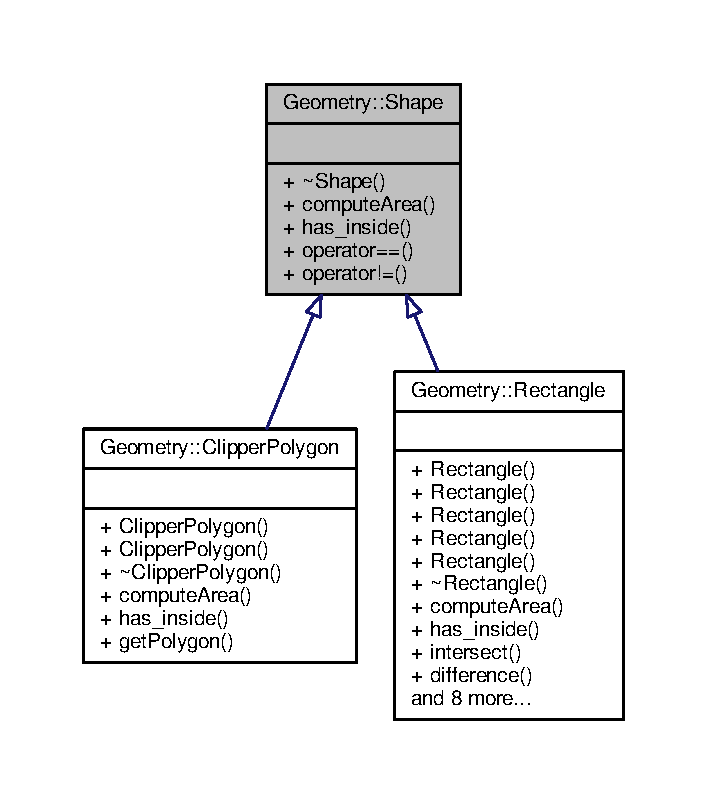
\includegraphics[width=340pt]{classGeometry_1_1Shape__inherit__graph}
\end{center}
\end{figure}


Collaboration diagram for Geometry\+:\+:Shape\+:\nopagebreak
\begin{figure}[H]
\begin{center}
\leavevmode
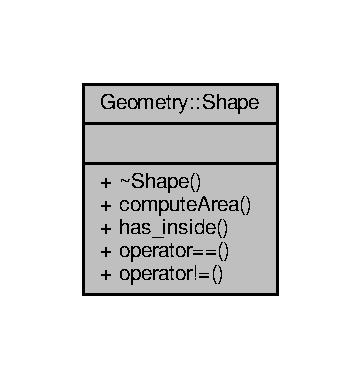
\includegraphics[width=173pt]{classGeometry_1_1Shape__coll__graph}
\end{center}
\end{figure}
\subsection*{Public Member Functions}
\begin{DoxyCompactItemize}
\item 
virtual \hyperlink{classGeometry_1_1Shape_a2f668d80c0a457a81a96de0253cfc67d}{$\sim$\+Shape} ()=default
\item 
virtual double \hyperlink{classGeometry_1_1Shape_ad0fb97e79dc8c171482bc14726ad8ce7}{compute\+Area} () const =0
\begin{DoxyCompactList}\small\item\em Get the area of the shape. \end{DoxyCompactList}\item 
virtual bool \hyperlink{classGeometry_1_1Shape_a2e1341ab60671a72a96bca2238cd38f0}{has\+\_\+inside} (\hyperlink{classGeometry_1_1Point2D}{Point2D} p) const =0
\begin{DoxyCompactList}\small\item\em Check if the point is inside the current shape. \end{DoxyCompactList}\item 
bool \hyperlink{classGeometry_1_1Shape_a9660f59db5df18d8ad95cd8d73edeb17}{operator==} (const \hyperlink{classGeometry_1_1Shape}{Shape} \&rhs) const 
\item 
bool \hyperlink{classGeometry_1_1Shape_aae9ac7a4269aeb197ec92a2d4230c178}{operator!=} (const \hyperlink{classGeometry_1_1Shape}{Shape} \&rhs) const 
\end{DoxyCompactItemize}


\subsection{Detailed Description}
Generic shape. 

\subsection{Constructor \& Destructor Documentation}
\index{Geometry\+::\+Shape@{Geometry\+::\+Shape}!````~Shape@{$\sim$\+Shape}}
\index{````~Shape@{$\sim$\+Shape}!Geometry\+::\+Shape@{Geometry\+::\+Shape}}
\subsubsection[{\texorpdfstring{$\sim$\+Shape()=default}{~Shape()=default}}]{\setlength{\rightskip}{0pt plus 5cm}virtual Geometry\+::\+Shape\+::$\sim$\+Shape (
\begin{DoxyParamCaption}
{}
\end{DoxyParamCaption}
)\hspace{0.3cm}{\ttfamily [virtual]}, {\ttfamily [default]}}\hypertarget{classGeometry_1_1Shape_a2f668d80c0a457a81a96de0253cfc67d}{}\label{classGeometry_1_1Shape_a2f668d80c0a457a81a96de0253cfc67d}


\subsection{Member Function Documentation}
\index{Geometry\+::\+Shape@{Geometry\+::\+Shape}!compute\+Area@{compute\+Area}}
\index{compute\+Area@{compute\+Area}!Geometry\+::\+Shape@{Geometry\+::\+Shape}}
\subsubsection[{\texorpdfstring{compute\+Area() const =0}{computeArea() const =0}}]{\setlength{\rightskip}{0pt plus 5cm}virtual double Geometry\+::\+Shape\+::compute\+Area (
\begin{DoxyParamCaption}
{}
\end{DoxyParamCaption}
) const\hspace{0.3cm}{\ttfamily [pure virtual]}}\hypertarget{classGeometry_1_1Shape_ad0fb97e79dc8c171482bc14726ad8ce7}{}\label{classGeometry_1_1Shape_ad0fb97e79dc8c171482bc14726ad8ce7}


Get the area of the shape. 

\begin{DoxyReturn}{Returns}
Area. 
\end{DoxyReturn}


Implemented in \hyperlink{classGeometry_1_1Rectangle_adcae3b63e18582f1d4983dfa80029fb7}{Geometry\+::\+Rectangle}, and \hyperlink{classGeometry_1_1ClipperPolygon_a452292446e85bf39afc64350180a289a}{Geometry\+::\+Clipper\+Polygon}.

\index{Geometry\+::\+Shape@{Geometry\+::\+Shape}!has\+\_\+inside@{has\+\_\+inside}}
\index{has\+\_\+inside@{has\+\_\+inside}!Geometry\+::\+Shape@{Geometry\+::\+Shape}}
\subsubsection[{\texorpdfstring{has\+\_\+inside(\+Point2\+D p) const =0}{has_inside(Point2D p) const =0}}]{\setlength{\rightskip}{0pt plus 5cm}virtual bool Geometry\+::\+Shape\+::has\+\_\+inside (
\begin{DoxyParamCaption}
\item[{{\bf Point2D}}]{p}
\end{DoxyParamCaption}
) const\hspace{0.3cm}{\ttfamily [pure virtual]}}\hypertarget{classGeometry_1_1Shape_a2e1341ab60671a72a96bca2238cd38f0}{}\label{classGeometry_1_1Shape_a2e1341ab60671a72a96bca2238cd38f0}


Check if the point is inside the current shape. 


\begin{DoxyParams}{Parameters}
{\em p} & Test point. \\
\hline
\end{DoxyParams}
\begin{DoxyReturn}{Returns}
True if p is inside the shape. 
\end{DoxyReturn}


Implemented in \hyperlink{classGeometry_1_1Rectangle_ab186008b8f7c4b99fec564021c40e3eb}{Geometry\+::\+Rectangle}, and \hyperlink{classGeometry_1_1ClipperPolygon_a8e863b1d54c4ccc8c9d84bcccbbb137f}{Geometry\+::\+Clipper\+Polygon}.

\index{Geometry\+::\+Shape@{Geometry\+::\+Shape}!operator"!=@{operator"!=}}
\index{operator"!=@{operator"!=}!Geometry\+::\+Shape@{Geometry\+::\+Shape}}
\subsubsection[{\texorpdfstring{operator"!=(const Shape \&rhs) const }{operator!=(const Shape &rhs) const }}]{\setlength{\rightskip}{0pt plus 5cm}bool Geometry\+::\+Shape\+::operator!= (
\begin{DoxyParamCaption}
\item[{const {\bf Shape} \&}]{rhs}
\end{DoxyParamCaption}
) const\hspace{0.3cm}{\ttfamily [inline]}}\hypertarget{classGeometry_1_1Shape_aae9ac7a4269aeb197ec92a2d4230c178}{}\label{classGeometry_1_1Shape_aae9ac7a4269aeb197ec92a2d4230c178}
\index{Geometry\+::\+Shape@{Geometry\+::\+Shape}!operator==@{operator==}}
\index{operator==@{operator==}!Geometry\+::\+Shape@{Geometry\+::\+Shape}}
\subsubsection[{\texorpdfstring{operator==(const Shape \&rhs) const }{operator==(const Shape &rhs) const }}]{\setlength{\rightskip}{0pt plus 5cm}bool Geometry\+::\+Shape\+::operator== (
\begin{DoxyParamCaption}
\item[{const {\bf Shape} \&}]{rhs}
\end{DoxyParamCaption}
) const\hspace{0.3cm}{\ttfamily [inline]}}\hypertarget{classGeometry_1_1Shape_a9660f59db5df18d8ad95cd8d73edeb17}{}\label{classGeometry_1_1Shape_a9660f59db5df18d8ad95cd8d73edeb17}


The documentation for this class was generated from the following file\+:\begin{DoxyCompactItemize}
\item 
geometry/\hyperlink{Shape_8h}{Shape.\+h}\end{DoxyCompactItemize}

\hypertarget{classUnidimensionalFocalElement}{}\section{Unidimensional\+Focal\+Element Class Reference}
\label{classUnidimensionalFocalElement}\index{Unidimensional\+Focal\+Element@{Unidimensional\+Focal\+Element}}


{\ttfamily \#include $<$Unidimensional\+Focal\+Element.\+h$>$}



Inheritance diagram for Unidimensional\+Focal\+Element\+:\nopagebreak
\begin{figure}[H]
\begin{center}
\leavevmode
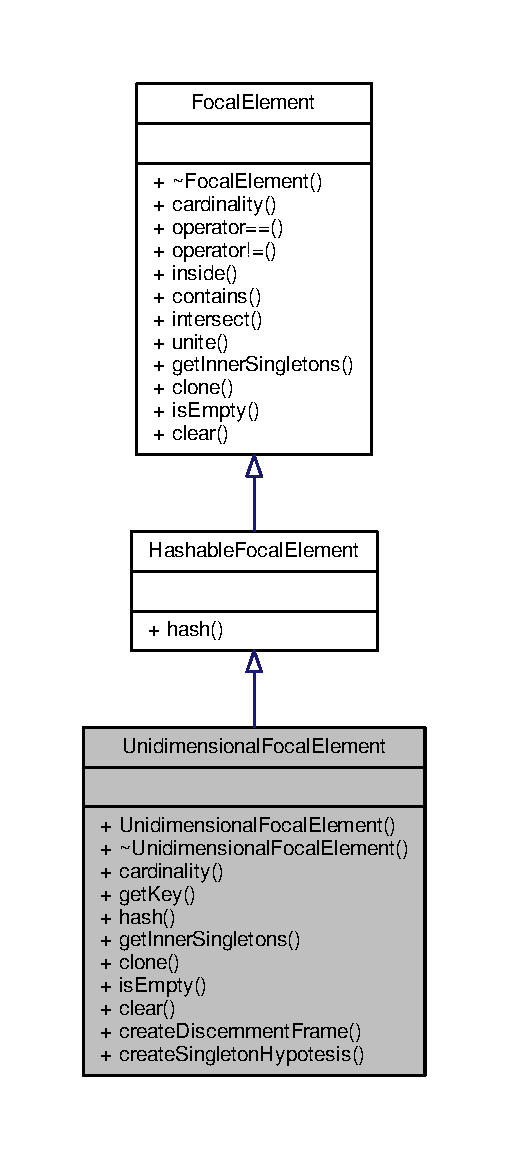
\includegraphics[height=550pt]{classUnidimensionalFocalElement__inherit__graph}
\end{center}
\end{figure}


Collaboration diagram for Unidimensional\+Focal\+Element\+:\nopagebreak
\begin{figure}[H]
\begin{center}
\leavevmode
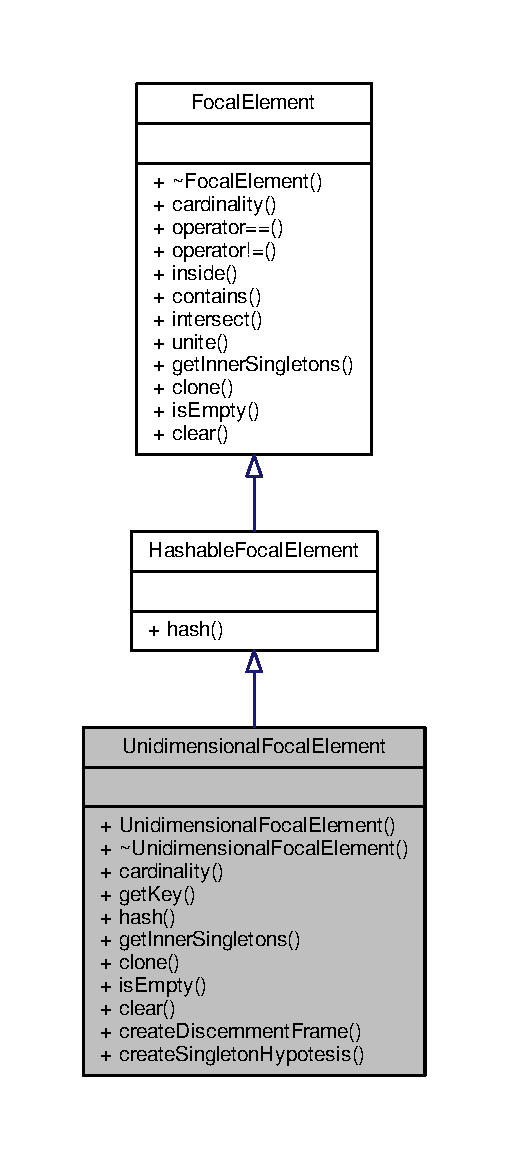
\includegraphics[height=550pt]{classUnidimensionalFocalElement__coll__graph}
\end{center}
\end{figure}
\subsection*{Public Member Functions}
\begin{DoxyCompactItemize}
\item 
\hyperlink{classUnidimensionalFocalElement_a634c688c14ef7a5a561dedf62e4cb0c3}{Unidimensional\+Focal\+Element} (unsigned long long I\+D)
\item 
\hyperlink{classUnidimensionalFocalElement_a0750b8a513e6ca16fdb94ff8012b78de}{$\sim$\+Unidimensional\+Focal\+Element} () override=default
\item 
double \hyperlink{classUnidimensionalFocalElement_a22e013e2875cf07f23b3fe8ab2e2431f}{cardinality} () const override
\item 
unsigned long long \hyperlink{classUnidimensionalFocalElement_a398bbc7cb6cabc000e549161323c3cf4}{get\+Key} () const 
\item 
size\+\_\+t \hyperlink{classUnidimensionalFocalElement_a073ce6e51cb7fff32b53e5f7b1d729c7}{hash} () const override
\item 
std\+::vector$<$ std\+::unique\+\_\+ptr$<$ \hyperlink{classFocalElement}{Focal\+Element} $>$ $>$ \hyperlink{classUnidimensionalFocalElement_ad37dc12733140cfd631d451ebfefcaf7}{get\+Inner\+Singletons} (int step\+\_\+size=1) const override
\item 
std\+::unique\+\_\+ptr$<$ \hyperlink{classFocalElement}{Focal\+Element} $>$ \hyperlink{classUnidimensionalFocalElement_aa06e27bc6c262783704883477d630d60}{clone} () const override
\item 
bool \hyperlink{classUnidimensionalFocalElement_a836c8a041ffba3e3e2ff7e584469a650}{is\+Empty} () const override
\item 
void \hyperlink{classUnidimensionalFocalElement_a1bd0c21e3e7e5a3ef78f4b47b98b6202}{clear} () override
\end{DoxyCompactItemize}
\subsection*{Static Public Member Functions}
\begin{DoxyCompactItemize}
\item 
static std\+::unique\+\_\+ptr$<$ \hyperlink{classUnidimensionalFocalElement}{Unidimensional\+Focal\+Element} $>$ \hyperlink{classUnidimensionalFocalElement_aba30678a3cd2534ea8becf0229fdb399}{create\+Discernment\+Frame} (unsigned char card)
\item 
static std\+::unique\+\_\+ptr$<$ \hyperlink{classUnidimensionalFocalElement}{Unidimensional\+Focal\+Element} $>$ \hyperlink{classUnidimensionalFocalElement_aa99e8f904b1cfdc880b41a36defe8aa5}{create\+Singleton\+Hypotesis} (size\+\_\+t hypotesis\+\_\+number)
\end{DoxyCompactItemize}


\subsection{Constructor \& Destructor Documentation}
\hypertarget{classUnidimensionalFocalElement_a634c688c14ef7a5a561dedf62e4cb0c3}{}\index{Unidimensional\+Focal\+Element@{Unidimensional\+Focal\+Element}!Unidimensional\+Focal\+Element@{Unidimensional\+Focal\+Element}}
\index{Unidimensional\+Focal\+Element@{Unidimensional\+Focal\+Element}!Unidimensional\+Focal\+Element@{Unidimensional\+Focal\+Element}}
\subsubsection[{Unidimensional\+Focal\+Element}]{\setlength{\rightskip}{0pt plus 5cm}Unidimensional\+Focal\+Element\+::\+Unidimensional\+Focal\+Element (
\begin{DoxyParamCaption}
\item[{unsigned long long}]{I\+D}
\end{DoxyParamCaption}
)\hspace{0.3cm}{\ttfamily [inline]}, {\ttfamily [explicit]}}\label{classUnidimensionalFocalElement_a634c688c14ef7a5a561dedf62e4cb0c3}
\hypertarget{classUnidimensionalFocalElement_a0750b8a513e6ca16fdb94ff8012b78de}{}\index{Unidimensional\+Focal\+Element@{Unidimensional\+Focal\+Element}!````~Unidimensional\+Focal\+Element@{$\sim$\+Unidimensional\+Focal\+Element}}
\index{````~Unidimensional\+Focal\+Element@{$\sim$\+Unidimensional\+Focal\+Element}!Unidimensional\+Focal\+Element@{Unidimensional\+Focal\+Element}}
\subsubsection[{$\sim$\+Unidimensional\+Focal\+Element}]{\setlength{\rightskip}{0pt plus 5cm}Unidimensional\+Focal\+Element\+::$\sim$\+Unidimensional\+Focal\+Element (
\begin{DoxyParamCaption}
{}
\end{DoxyParamCaption}
)\hspace{0.3cm}{\ttfamily [override]}, {\ttfamily [default]}}\label{classUnidimensionalFocalElement_a0750b8a513e6ca16fdb94ff8012b78de}


\subsection{Member Function Documentation}
\hypertarget{classUnidimensionalFocalElement_a22e013e2875cf07f23b3fe8ab2e2431f}{}\index{Unidimensional\+Focal\+Element@{Unidimensional\+Focal\+Element}!cardinality@{cardinality}}
\index{cardinality@{cardinality}!Unidimensional\+Focal\+Element@{Unidimensional\+Focal\+Element}}
\subsubsection[{cardinality}]{\setlength{\rightskip}{0pt plus 5cm}double Unidimensional\+Focal\+Element\+::cardinality (
\begin{DoxyParamCaption}
{}
\end{DoxyParamCaption}
) const\hspace{0.3cm}{\ttfamily [override]}, {\ttfamily [virtual]}}\label{classUnidimensionalFocalElement_a22e013e2875cf07f23b3fe8ab2e2431f}


Implements \hyperlink{classFocalElement_a4ab1bbd0875e6e7ce2d7fe152e6a1639}{Focal\+Element}.

\hypertarget{classUnidimensionalFocalElement_a1bd0c21e3e7e5a3ef78f4b47b98b6202}{}\index{Unidimensional\+Focal\+Element@{Unidimensional\+Focal\+Element}!clear@{clear}}
\index{clear@{clear}!Unidimensional\+Focal\+Element@{Unidimensional\+Focal\+Element}}
\subsubsection[{clear}]{\setlength{\rightskip}{0pt plus 5cm}void Unidimensional\+Focal\+Element\+::clear (
\begin{DoxyParamCaption}
{}
\end{DoxyParamCaption}
)\hspace{0.3cm}{\ttfamily [override]}, {\ttfamily [virtual]}}\label{classUnidimensionalFocalElement_a1bd0c21e3e7e5a3ef78f4b47b98b6202}


Implements \hyperlink{classFocalElement_a635cb4afffa2dc69cf9fc9ff94a6d90f}{Focal\+Element}.

\hypertarget{classUnidimensionalFocalElement_aa06e27bc6c262783704883477d630d60}{}\index{Unidimensional\+Focal\+Element@{Unidimensional\+Focal\+Element}!clone@{clone}}
\index{clone@{clone}!Unidimensional\+Focal\+Element@{Unidimensional\+Focal\+Element}}
\subsubsection[{clone}]{\setlength{\rightskip}{0pt plus 5cm}std\+::unique\+\_\+ptr$<$ {\bf Focal\+Element} $>$ Unidimensional\+Focal\+Element\+::clone (
\begin{DoxyParamCaption}
{}
\end{DoxyParamCaption}
) const\hspace{0.3cm}{\ttfamily [override]}, {\ttfamily [virtual]}}\label{classUnidimensionalFocalElement_aa06e27bc6c262783704883477d630d60}


Implements \hyperlink{classFocalElement_a21697fbbbcb144c18fa7b4ecae5e6145}{Focal\+Element}.

\hypertarget{classUnidimensionalFocalElement_aba30678a3cd2534ea8becf0229fdb399}{}\index{Unidimensional\+Focal\+Element@{Unidimensional\+Focal\+Element}!create\+Discernment\+Frame@{create\+Discernment\+Frame}}
\index{create\+Discernment\+Frame@{create\+Discernment\+Frame}!Unidimensional\+Focal\+Element@{Unidimensional\+Focal\+Element}}
\subsubsection[{create\+Discernment\+Frame}]{\setlength{\rightskip}{0pt plus 5cm}std\+::unique\+\_\+ptr$<$ {\bf Unidimensional\+Focal\+Element} $>$ Unidimensional\+Focal\+Element\+::create\+Discernment\+Frame (
\begin{DoxyParamCaption}
\item[{unsigned char}]{card}
\end{DoxyParamCaption}
)\hspace{0.3cm}{\ttfamily [static]}}\label{classUnidimensionalFocalElement_aba30678a3cd2534ea8becf0229fdb399}
\hypertarget{classUnidimensionalFocalElement_aa99e8f904b1cfdc880b41a36defe8aa5}{}\index{Unidimensional\+Focal\+Element@{Unidimensional\+Focal\+Element}!create\+Singleton\+Hypotesis@{create\+Singleton\+Hypotesis}}
\index{create\+Singleton\+Hypotesis@{create\+Singleton\+Hypotesis}!Unidimensional\+Focal\+Element@{Unidimensional\+Focal\+Element}}
\subsubsection[{create\+Singleton\+Hypotesis}]{\setlength{\rightskip}{0pt plus 5cm}std\+::unique\+\_\+ptr$<$ {\bf Unidimensional\+Focal\+Element} $>$ Unidimensional\+Focal\+Element\+::create\+Singleton\+Hypotesis (
\begin{DoxyParamCaption}
\item[{size\+\_\+t}]{hypotesis\+\_\+number}
\end{DoxyParamCaption}
)\hspace{0.3cm}{\ttfamily [static]}}\label{classUnidimensionalFocalElement_aa99e8f904b1cfdc880b41a36defe8aa5}
\hypertarget{classUnidimensionalFocalElement_ad37dc12733140cfd631d451ebfefcaf7}{}\index{Unidimensional\+Focal\+Element@{Unidimensional\+Focal\+Element}!get\+Inner\+Singletons@{get\+Inner\+Singletons}}
\index{get\+Inner\+Singletons@{get\+Inner\+Singletons}!Unidimensional\+Focal\+Element@{Unidimensional\+Focal\+Element}}
\subsubsection[{get\+Inner\+Singletons}]{\setlength{\rightskip}{0pt plus 5cm}std\+::vector$<$ std\+::unique\+\_\+ptr$<$ {\bf Focal\+Element} $>$ $>$ Unidimensional\+Focal\+Element\+::get\+Inner\+Singletons (
\begin{DoxyParamCaption}
\item[{int}]{step\+\_\+size = {\ttfamily 1}}
\end{DoxyParamCaption}
) const\hspace{0.3cm}{\ttfamily [override]}, {\ttfamily [virtual]}}\label{classUnidimensionalFocalElement_ad37dc12733140cfd631d451ebfefcaf7}


Implements \hyperlink{classFocalElement_ac615e960ea64a4bdc0f442135f6069e2}{Focal\+Element}.

\hypertarget{classUnidimensionalFocalElement_a398bbc7cb6cabc000e549161323c3cf4}{}\index{Unidimensional\+Focal\+Element@{Unidimensional\+Focal\+Element}!get\+Key@{get\+Key}}
\index{get\+Key@{get\+Key}!Unidimensional\+Focal\+Element@{Unidimensional\+Focal\+Element}}
\subsubsection[{get\+Key}]{\setlength{\rightskip}{0pt plus 5cm}unsigned long long Unidimensional\+Focal\+Element\+::get\+Key (
\begin{DoxyParamCaption}
{}
\end{DoxyParamCaption}
) const}\label{classUnidimensionalFocalElement_a398bbc7cb6cabc000e549161323c3cf4}
\hypertarget{classUnidimensionalFocalElement_a073ce6e51cb7fff32b53e5f7b1d729c7}{}\index{Unidimensional\+Focal\+Element@{Unidimensional\+Focal\+Element}!hash@{hash}}
\index{hash@{hash}!Unidimensional\+Focal\+Element@{Unidimensional\+Focal\+Element}}
\subsubsection[{hash}]{\setlength{\rightskip}{0pt plus 5cm}size\+\_\+t Unidimensional\+Focal\+Element\+::hash (
\begin{DoxyParamCaption}
{}
\end{DoxyParamCaption}
) const\hspace{0.3cm}{\ttfamily [override]}, {\ttfamily [virtual]}}\label{classUnidimensionalFocalElement_a073ce6e51cb7fff32b53e5f7b1d729c7}


Implements \hyperlink{classHashableFocalElement_a8b7bfbf1e107fa5a6cfc5033db196c63}{Hashable\+Focal\+Element}.

\hypertarget{classUnidimensionalFocalElement_a836c8a041ffba3e3e2ff7e584469a650}{}\index{Unidimensional\+Focal\+Element@{Unidimensional\+Focal\+Element}!is\+Empty@{is\+Empty}}
\index{is\+Empty@{is\+Empty}!Unidimensional\+Focal\+Element@{Unidimensional\+Focal\+Element}}
\subsubsection[{is\+Empty}]{\setlength{\rightskip}{0pt plus 5cm}bool Unidimensional\+Focal\+Element\+::is\+Empty (
\begin{DoxyParamCaption}
{}
\end{DoxyParamCaption}
) const\hspace{0.3cm}{\ttfamily [override]}, {\ttfamily [virtual]}}\label{classUnidimensionalFocalElement_a836c8a041ffba3e3e2ff7e584469a650}


Implements \hyperlink{classFocalElement_aed131a65fdfc885019f9bf8f1d454508}{Focal\+Element}.



The documentation for this class was generated from the following files\+:\begin{DoxyCompactItemize}
\item 
focal\+\_\+elements/\hyperlink{UnidimensionalFocalElement_8h}{Unidimensional\+Focal\+Element.\+h}\item 
focal\+\_\+elements/\hyperlink{UnidimensionalFocalElement_8cpp}{Unidimensional\+Focal\+Element.\+cpp}\end{DoxyCompactItemize}

\chapter{File Documentation}
\hypertarget{DefaultFocalElementContainerDispatcher_8cpp}{}\section{containers/\+Default\+Focal\+Element\+Container\+Dispatcher.cpp File Reference}
\label{DefaultFocalElementContainerDispatcher_8cpp}\index{containers/\+Default\+Focal\+Element\+Container\+Dispatcher.\+cpp@{containers/\+Default\+Focal\+Element\+Container\+Dispatcher.\+cpp}}
{\ttfamily \#include \char`\"{}../focal\+\_\+elements/\+Hashable\+Focal\+Element.\+h\char`\"{}}\\*
{\ttfamily \#include \char`\"{}Default\+Focal\+Element\+Container\+Dispatcher.\+h\char`\"{}}\\*
{\ttfamily \#include \char`\"{}Generic\+Focal\+Element\+Container.\+h\char`\"{}}\\*
{\ttfamily \#include \char`\"{}Hashable\+Focal\+Element\+Container.\+h\char`\"{}}\\*
Include dependency graph for Default\+Focal\+Element\+Container\+Dispatcher.\+cpp\+:\nopagebreak
\begin{figure}[H]
\begin{center}
\leavevmode
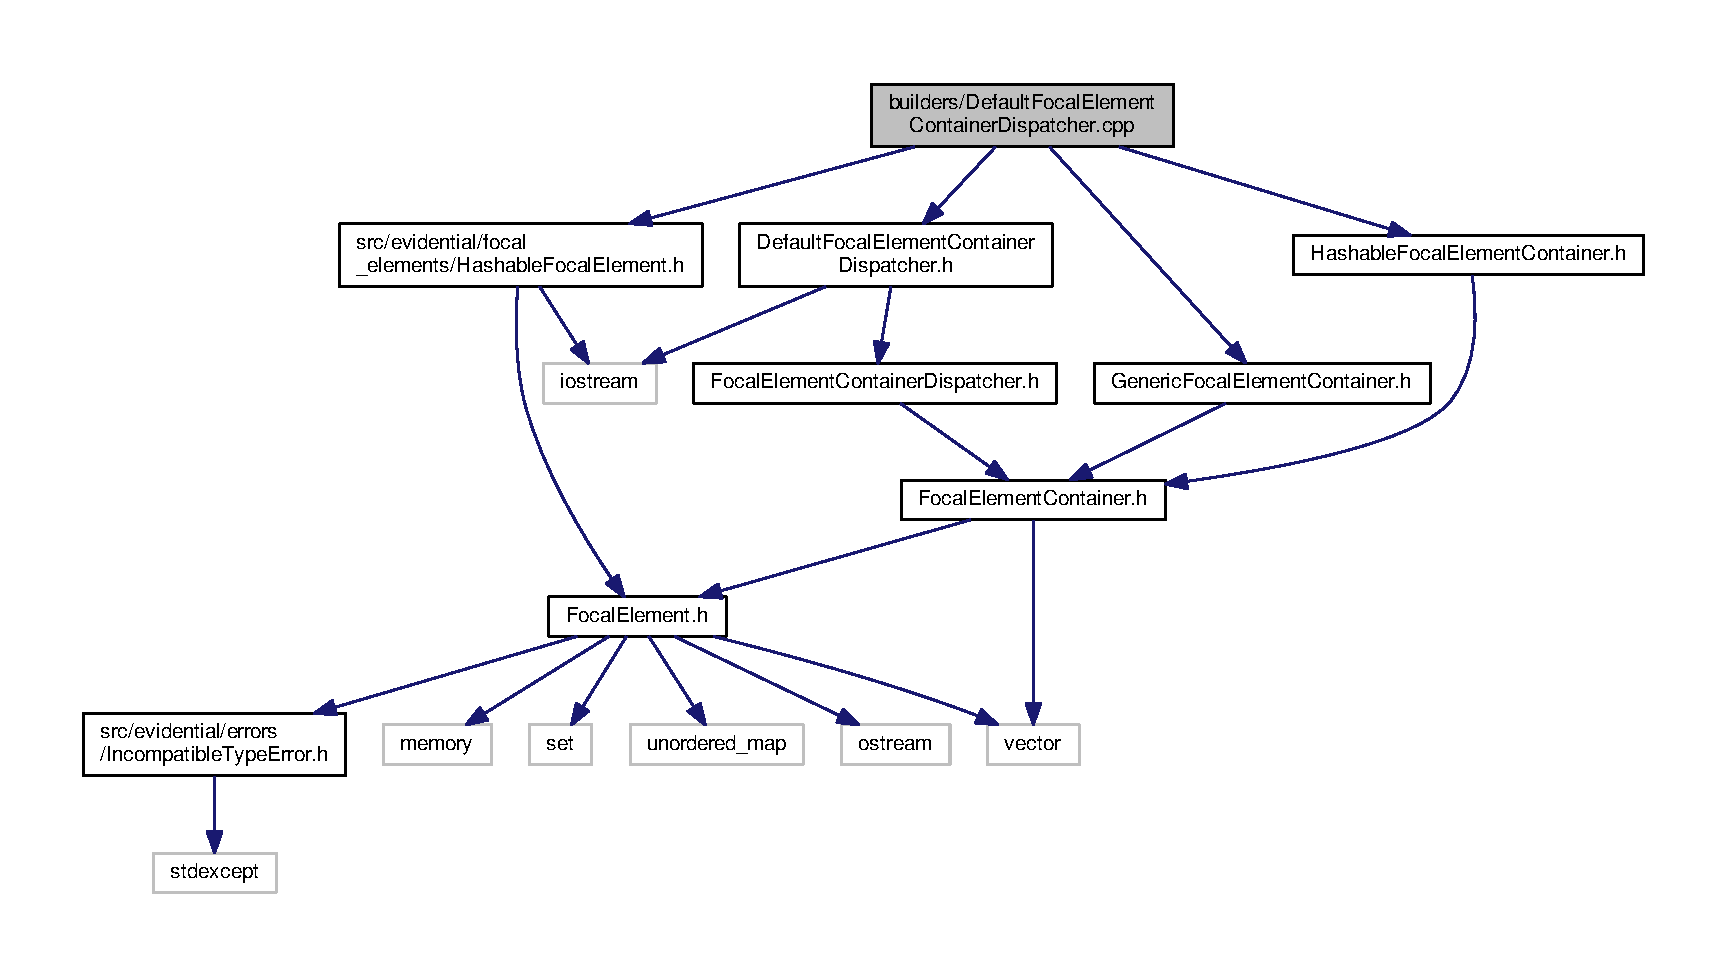
\includegraphics[width=350pt]{DefaultFocalElementContainerDispatcher_8cpp__incl}
\end{center}
\end{figure}

\hypertarget{DefaultFocalElementContainerDispatcher_8h}{}\section{containers/\+Default\+Focal\+Element\+Container\+Dispatcher.h File Reference}
\label{DefaultFocalElementContainerDispatcher_8h}\index{containers/\+Default\+Focal\+Element\+Container\+Dispatcher.\+h@{containers/\+Default\+Focal\+Element\+Container\+Dispatcher.\+h}}
{\ttfamily \#include $<$iostream$>$}\\*
{\ttfamily \#include \char`\"{}Focal\+Element\+Container\+Dispatcher.\+h\char`\"{}}\\*
Include dependency graph for Default\+Focal\+Element\+Container\+Dispatcher.\+h\+:\nopagebreak
\begin{figure}[H]
\begin{center}
\leavevmode
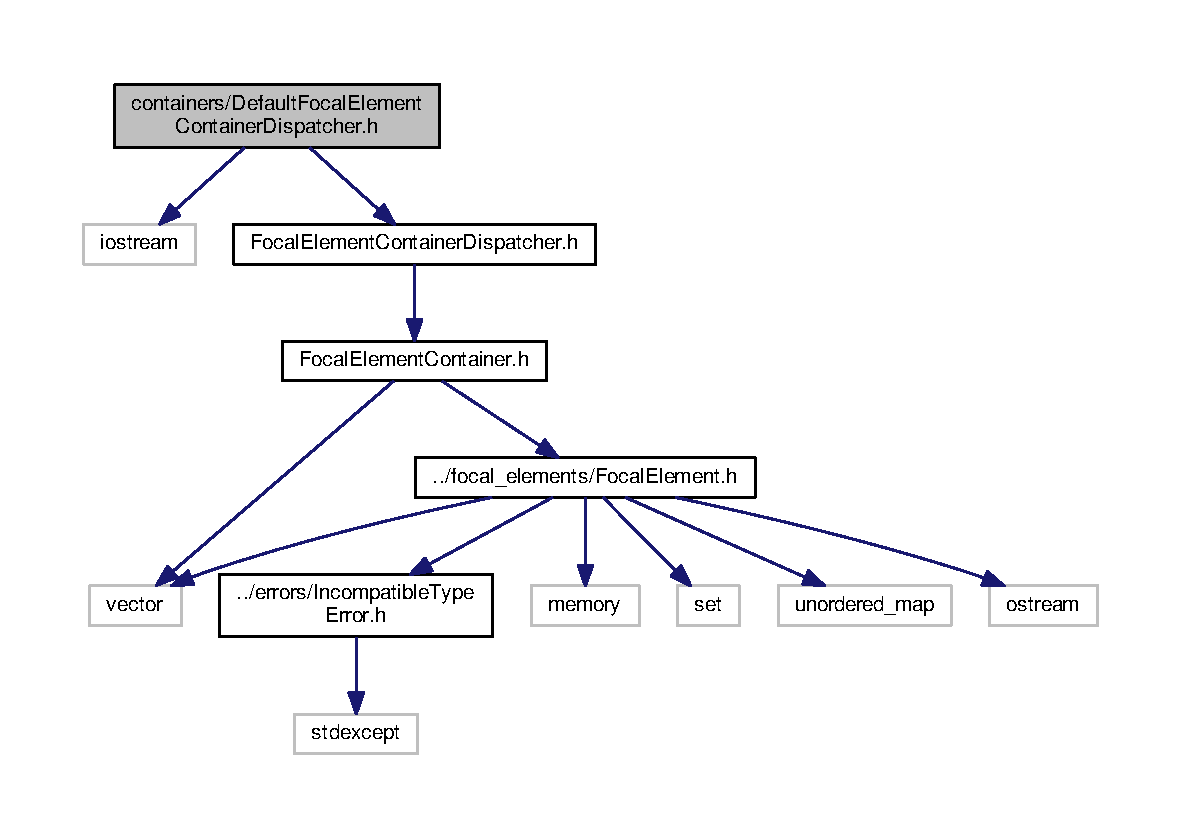
\includegraphics[width=350pt]{DefaultFocalElementContainerDispatcher_8h__incl}
\end{center}
\end{figure}
This graph shows which files directly or indirectly include this file\+:\nopagebreak
\begin{figure}[H]
\begin{center}
\leavevmode
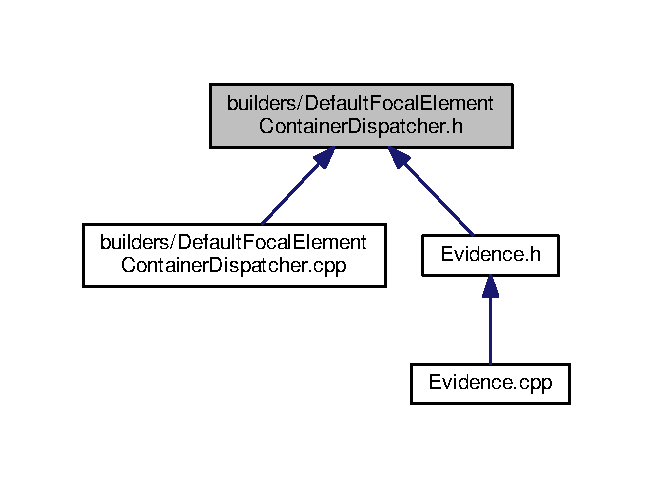
\includegraphics[width=350pt]{DefaultFocalElementContainerDispatcher_8h__dep__incl}
\end{center}
\end{figure}
\subsection*{Classes}
\begin{DoxyCompactItemize}
\item 
class \hyperlink{classDefaultFocalElementContainerDispatcher}{Default\+Focal\+Element\+Container\+Dispatcher}
\begin{DoxyCompactList}\small\item\em The default dispatcher for \hyperlink{classFocalElementContainer}{Focal\+Element\+Container}. \end{DoxyCompactList}\end{DoxyCompactItemize}

\hypertarget{FocalElementContainer_8h}{}\section{containers/\+Focal\+Element\+Container.h File Reference}
\label{FocalElementContainer_8h}\index{containers/\+Focal\+Element\+Container.\+h@{containers/\+Focal\+Element\+Container.\+h}}
{\ttfamily \#include $<$vector$>$}\\*
{\ttfamily \#include \char`\"{}../focal\+\_\+elements/\+Focal\+Element.\+h\char`\"{}}\\*
Include dependency graph for Focal\+Element\+Container.\+h\+:\nopagebreak
\begin{figure}[H]
\begin{center}
\leavevmode
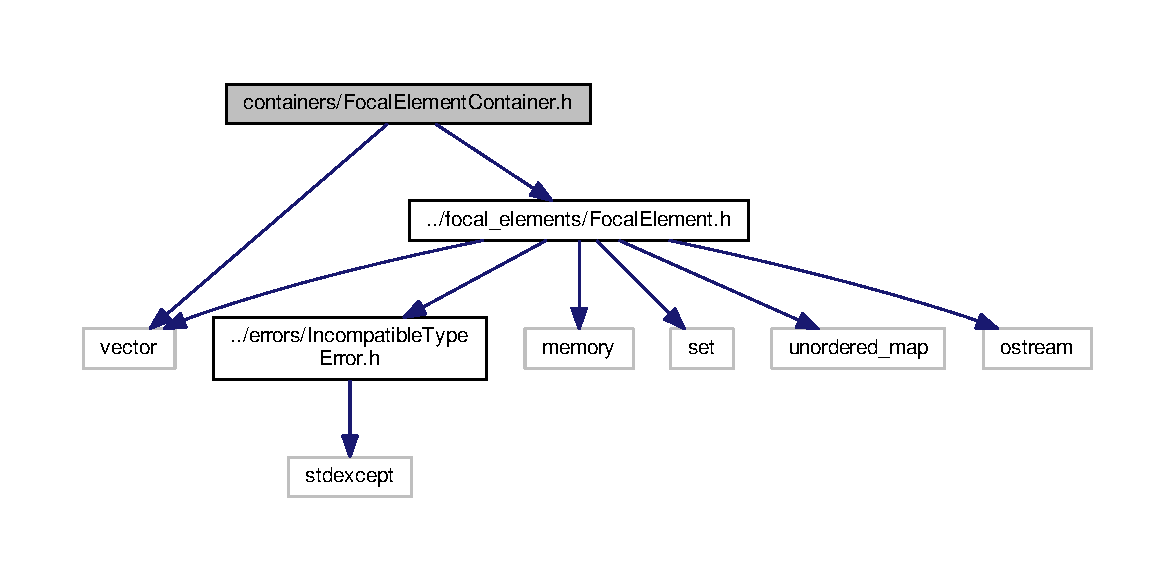
\includegraphics[width=350pt]{FocalElementContainer_8h__incl}
\end{center}
\end{figure}
This graph shows which files directly or indirectly include this file\+:
\nopagebreak
\begin{figure}[H]
\begin{center}
\leavevmode
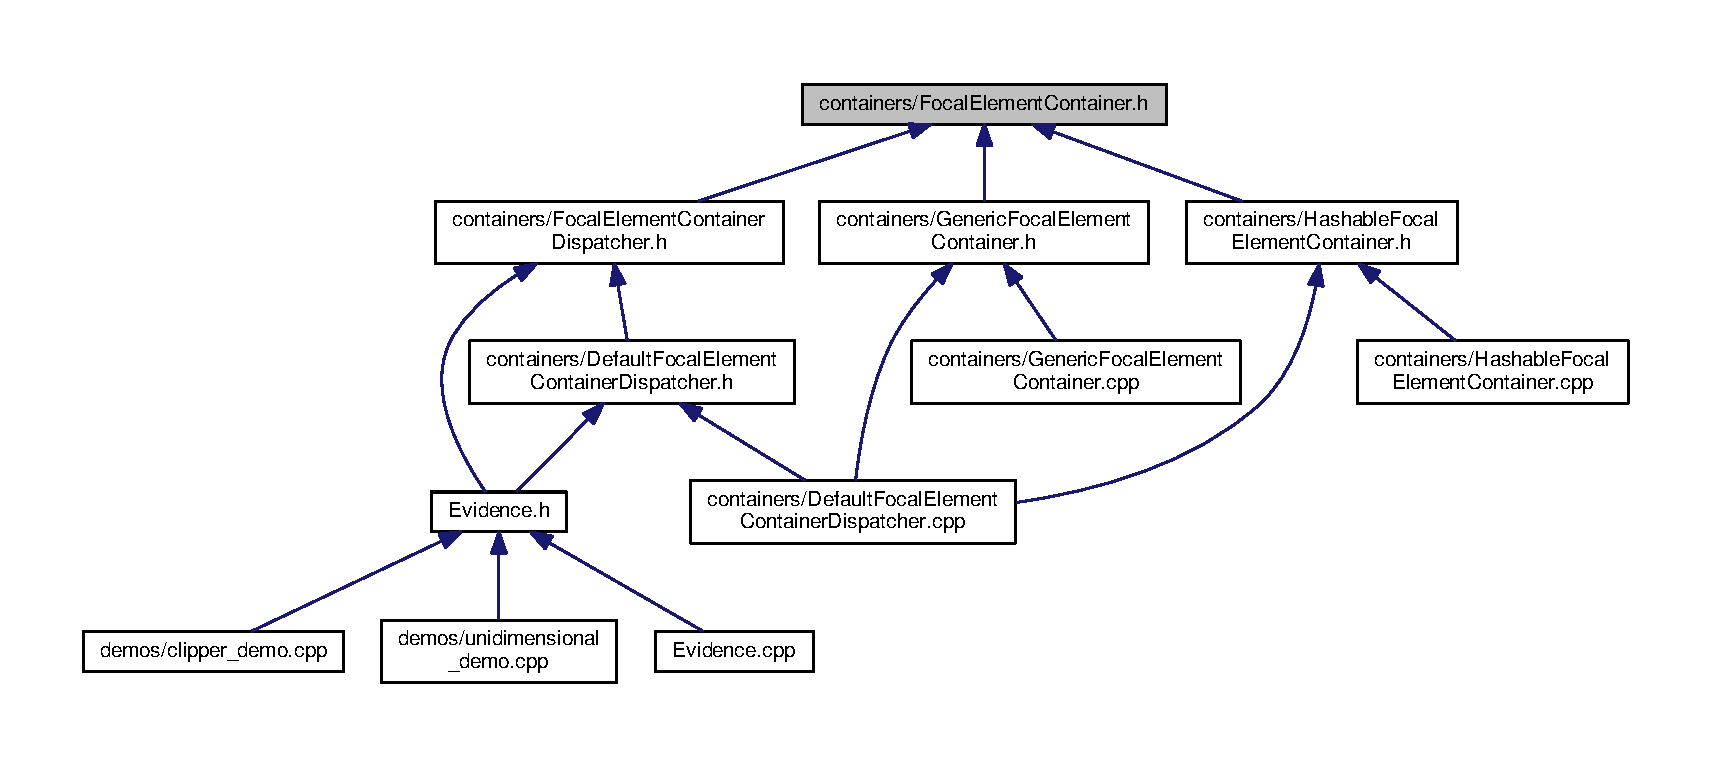
\includegraphics[width=350pt]{FocalElementContainer_8h__dep__incl}
\end{center}
\end{figure}
\subsection*{Classes}
\begin{DoxyCompactItemize}
\item 
class \hyperlink{classFocalElementContainer}{Focal\+Element\+Container}
\begin{DoxyCompactList}\small\item\em Container of \hyperlink{classFocalElement}{Focal\+Element} objects. \end{DoxyCompactList}\end{DoxyCompactItemize}

\hypertarget{FocalElementContainerDispatcher_8h}{}\section{containers/\+Focal\+Element\+Container\+Dispatcher.h File Reference}
\label{FocalElementContainerDispatcher_8h}\index{containers/\+Focal\+Element\+Container\+Dispatcher.\+h@{containers/\+Focal\+Element\+Container\+Dispatcher.\+h}}
{\ttfamily \#include \char`\"{}Focal\+Element\+Container.\+h\char`\"{}}\\*
Include dependency graph for Focal\+Element\+Container\+Dispatcher.\+h\+:\nopagebreak
\begin{figure}[H]
\begin{center}
\leavevmode
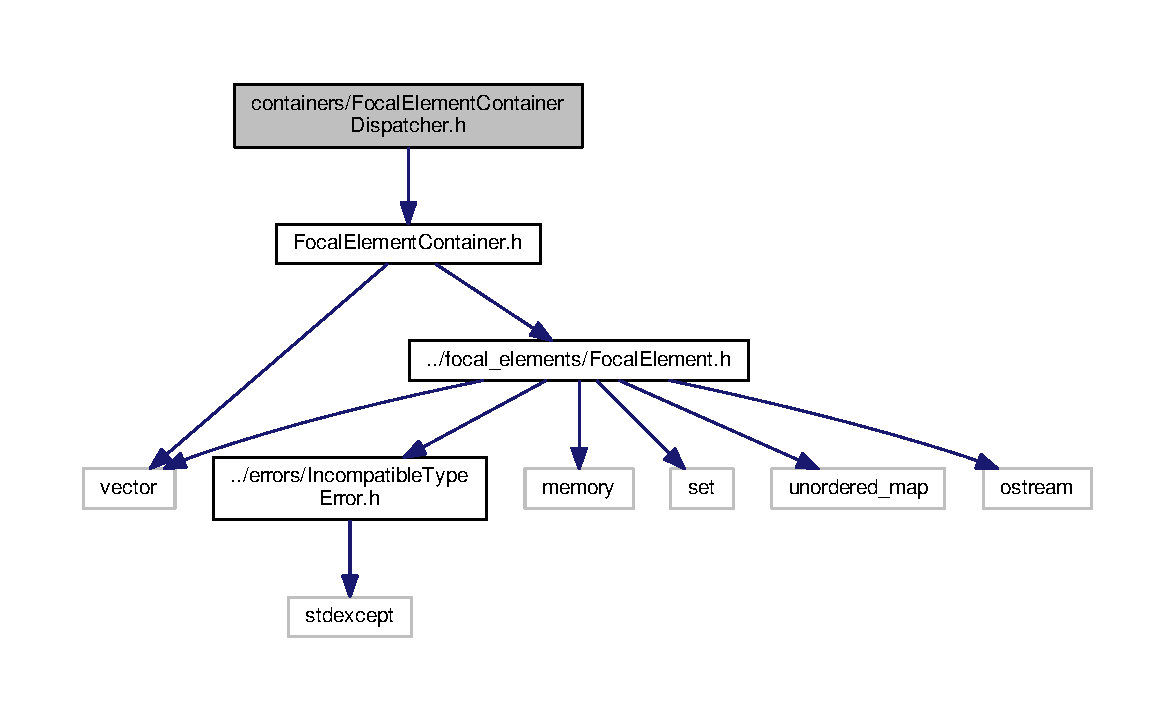
\includegraphics[width=350pt]{FocalElementContainerDispatcher_8h__incl}
\end{center}
\end{figure}
This graph shows which files directly or indirectly include this file\+:\nopagebreak
\begin{figure}[H]
\begin{center}
\leavevmode
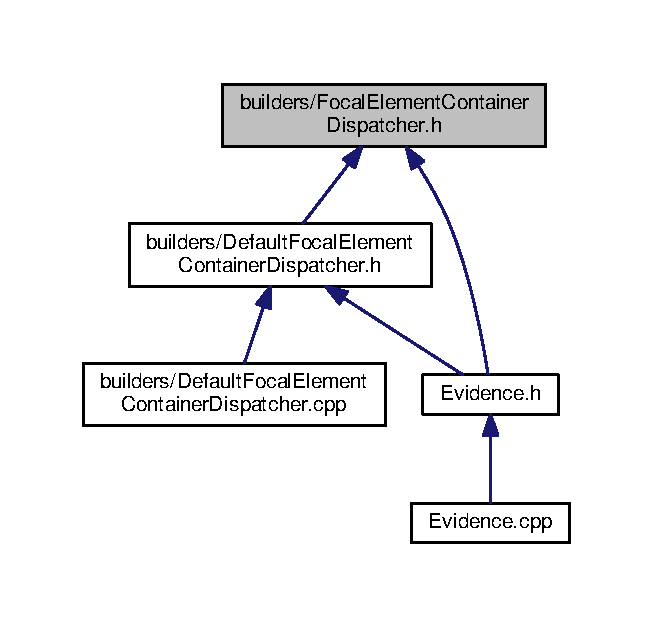
\includegraphics[width=350pt]{FocalElementContainerDispatcher_8h__dep__incl}
\end{center}
\end{figure}
\subsection*{Classes}
\begin{DoxyCompactItemize}
\item 
class \hyperlink{classFocalElementContainerDispatcher}{Focal\+Element\+Container\+Dispatcher}
\begin{DoxyCompactList}\small\item\em Dispatcher of the correct \hyperlink{classFocalElementContainer}{Focal\+Element\+Container}, given the \hyperlink{classFocalElement}{Focal\+Element} type. \end{DoxyCompactList}\end{DoxyCompactItemize}

\hypertarget{GenericFocalElementContainer_8cpp}{}\section{builders/\+Generic\+Focal\+Element\+Container.cpp File Reference}
\label{GenericFocalElementContainer_8cpp}\index{builders/\+Generic\+Focal\+Element\+Container.\+cpp@{builders/\+Generic\+Focal\+Element\+Container.\+cpp}}
{\ttfamily \#include $<$iostream$>$}\\*
{\ttfamily \#include $<$src/evidential/errors/\+Illegal\+Argument\+Error.\+h$>$}\\*
{\ttfamily \#include \char`\"{}Generic\+Focal\+Element\+Container.\+h\char`\"{}}\\*
Include dependency graph for Generic\+Focal\+Element\+Container.\+cpp\+:\nopagebreak
\begin{figure}[H]
\begin{center}
\leavevmode
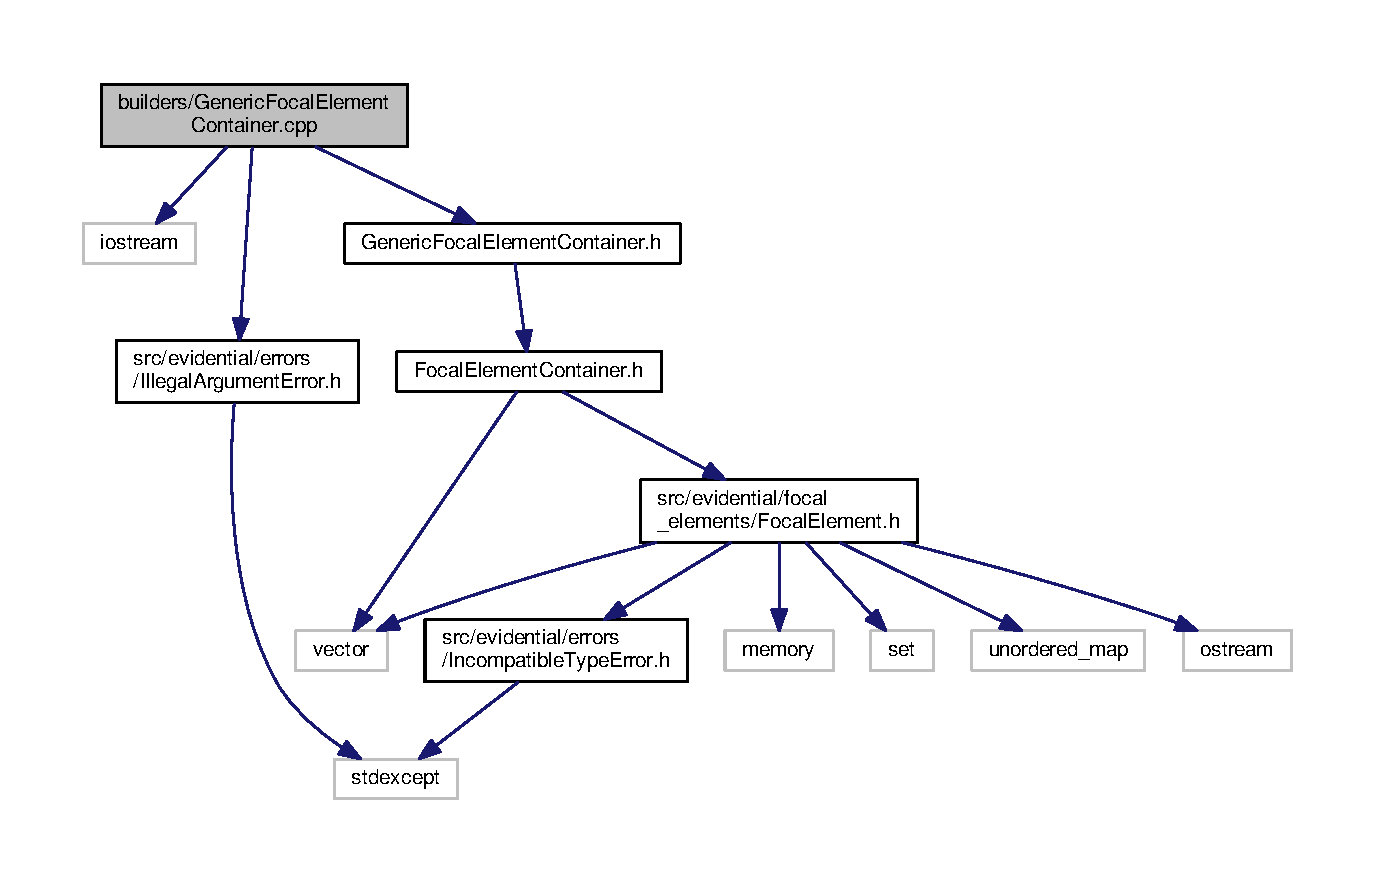
\includegraphics[width=350pt]{GenericFocalElementContainer_8cpp__incl}
\end{center}
\end{figure}

\hypertarget{GenericFocalElementContainer_8h}{}\section{containers/\+Generic\+Focal\+Element\+Container.h File Reference}
\label{GenericFocalElementContainer_8h}\index{containers/\+Generic\+Focal\+Element\+Container.\+h@{containers/\+Generic\+Focal\+Element\+Container.\+h}}
{\ttfamily \#include \char`\"{}Focal\+Element\+Container.\+h\char`\"{}}\\*
Include dependency graph for Generic\+Focal\+Element\+Container.\+h\+:\nopagebreak
\begin{figure}[H]
\begin{center}
\leavevmode
\includegraphics[width=350pt]{GenericFocalElementContainer_8h__incl}
\end{center}
\end{figure}
This graph shows which files directly or indirectly include this file\+:\nopagebreak
\begin{figure}[H]
\begin{center}
\leavevmode
\includegraphics[width=350pt]{GenericFocalElementContainer_8h__dep__incl}
\end{center}
\end{figure}
\subsection*{Classes}
\begin{DoxyCompactItemize}
\item 
class \hyperlink{classGenericFocalElementContainer}{Generic\+Focal\+Element\+Container}
\begin{DoxyCompactList}\small\item\em A container for any type of \hyperlink{classFocalElement}{Focal\+Element} object. \end{DoxyCompactList}\end{DoxyCompactItemize}

\hypertarget{HashableFocalElementContainer_8cpp}{}\section{builders/\+Hashable\+Focal\+Element\+Container.cpp File Reference}
\label{HashableFocalElementContainer_8cpp}\index{builders/\+Hashable\+Focal\+Element\+Container.\+cpp@{builders/\+Hashable\+Focal\+Element\+Container.\+cpp}}
{\ttfamily \#include $<$src/evidential/focal\+\_\+elements/\+Hashable\+Focal\+Element.\+h$>$}\\*
{\ttfamily \#include $<$src/evidential/errors/\+Illegal\+Argument\+Error.\+h$>$}\\*
{\ttfamily \#include \char`\"{}Hashable\+Focal\+Element\+Container.\+h\char`\"{}}\\*
Include dependency graph for Hashable\+Focal\+Element\+Container.\+cpp\+:\nopagebreak
\begin{figure}[H]
\begin{center}
\leavevmode
\includegraphics[width=350pt]{HashableFocalElementContainer_8cpp__incl}
\end{center}
\end{figure}

\hypertarget{HashableFocalElementContainer_8h}{}\section{containers/\+Hashable\+Focal\+Element\+Container.h File Reference}
\label{HashableFocalElementContainer_8h}\index{containers/\+Hashable\+Focal\+Element\+Container.\+h@{containers/\+Hashable\+Focal\+Element\+Container.\+h}}
{\ttfamily \#include \char`\"{}Focal\+Element\+Container.\+h\char`\"{}}\\*
Include dependency graph for Hashable\+Focal\+Element\+Container.\+h\+:\nopagebreak
\begin{figure}[H]
\begin{center}
\leavevmode
\includegraphics[width=350pt]{HashableFocalElementContainer_8h__incl}
\end{center}
\end{figure}
This graph shows which files directly or indirectly include this file\+:\nopagebreak
\begin{figure}[H]
\begin{center}
\leavevmode
\includegraphics[width=350pt]{HashableFocalElementContainer_8h__dep__incl}
\end{center}
\end{figure}
\subsection*{Classes}
\begin{DoxyCompactItemize}
\item 
class \hyperlink{classHashableFocalElementContainer}{Hashable\+Focal\+Element\+Container}
\begin{DoxyCompactList}\small\item\em A container for \hyperlink{classHashableFocalElement}{Hashable\+Focal\+Element} type objects. \end{DoxyCompactList}\end{DoxyCompactItemize}

\hypertarget{ConstructorArgumentsError_8h}{}\section{errors/\+Constructor\+Arguments\+Error.h File Reference}
\label{ConstructorArgumentsError_8h}\index{errors/\+Constructor\+Arguments\+Error.\+h@{errors/\+Constructor\+Arguments\+Error.\+h}}
{\ttfamily \#include $<$stdexcept$>$}\\*
Include dependency graph for Constructor\+Arguments\+Error.\+h\+:\nopagebreak
\begin{figure}[H]
\begin{center}
\leavevmode
\includegraphics[width=223pt]{ConstructorArgumentsError_8h__incl}
\end{center}
\end{figure}
This graph shows which files directly or indirectly include this file\+:\nopagebreak
\begin{figure}[H]
\begin{center}
\leavevmode
\includegraphics[width=350pt]{ConstructorArgumentsError_8h__dep__incl}
\end{center}
\end{figure}
\subsection*{Classes}
\begin{DoxyCompactItemize}
\item 
class \hyperlink{classConstructorArgumentsError}{Constructor\+Arguments\+Error}
\end{DoxyCompactItemize}

\hypertarget{IllegalArgumentError_8h}{}\section{errors/\+Illegal\+Argument\+Error.h File Reference}
\label{IllegalArgumentError_8h}\index{errors/\+Illegal\+Argument\+Error.\+h@{errors/\+Illegal\+Argument\+Error.\+h}}
{\ttfamily \#include $<$stdexcept$>$}\\*
Include dependency graph for Illegal\+Argument\+Error.\+h\+:\nopagebreak
\begin{figure}[H]
\begin{center}
\leavevmode
\includegraphics[width=221pt]{IllegalArgumentError_8h__incl}
\end{center}
\end{figure}
This graph shows which files directly or indirectly include this file\+:\nopagebreak
\begin{figure}[H]
\begin{center}
\leavevmode
\includegraphics[width=350pt]{IllegalArgumentError_8h__dep__incl}
\end{center}
\end{figure}
\subsection*{Classes}
\begin{DoxyCompactItemize}
\item 
class \hyperlink{classIllegalArgumentError}{Illegal\+Argument\+Error}
\begin{DoxyCompactList}\small\item\em Error in the parameter of a method. \end{DoxyCompactList}\end{DoxyCompactItemize}

\hypertarget{IncompatibleTypeError_8h}{}\section{errors/\+Incompatible\+Type\+Error.h File Reference}
\label{IncompatibleTypeError_8h}\index{errors/\+Incompatible\+Type\+Error.\+h@{errors/\+Incompatible\+Type\+Error.\+h}}
{\ttfamily \#include $<$stdexcept$>$}\\*
Include dependency graph for Incompatible\+Type\+Error.\+h\+:\nopagebreak
\begin{figure}[H]
\begin{center}
\leavevmode
\includegraphics[width=231pt]{IncompatibleTypeError_8h__incl}
\end{center}
\end{figure}
This graph shows which files directly or indirectly include this file\+:\nopagebreak
\begin{figure}[H]
\begin{center}
\leavevmode
\includegraphics[width=350pt]{IncompatibleTypeError_8h__dep__incl}
\end{center}
\end{figure}
\subsection*{Classes}
\begin{DoxyCompactItemize}
\item 
class \hyperlink{classIncompatibleTypeError}{Incompatible\+Type\+Error}
\begin{DoxyCompactList}\small\item\em Error in the type of an object. \end{DoxyCompactList}\end{DoxyCompactItemize}

\hypertarget{InvalidBBAError_8h}{}\section{errors/\+Invalid\+B\+B\+A\+Error.h File Reference}
\label{InvalidBBAError_8h}\index{errors/\+Invalid\+B\+B\+A\+Error.\+h@{errors/\+Invalid\+B\+B\+A\+Error.\+h}}
{\ttfamily \#include $<$stdexcept$>$}\\*
Include dependency graph for Invalid\+B\+B\+A\+Error.\+h\+:\nopagebreak
\begin{figure}[H]
\begin{center}
\leavevmode
\includegraphics[width=202pt]{InvalidBBAError_8h__incl}
\end{center}
\end{figure}
This graph shows which files directly or indirectly include this file\+:\nopagebreak
\begin{figure}[H]
\begin{center}
\leavevmode
\includegraphics[width=202pt]{InvalidBBAError_8h__dep__incl}
\end{center}
\end{figure}
\subsection*{Classes}
\begin{DoxyCompactItemize}
\item 
class \hyperlink{classInvalidBBAError}{Invalid\+B\+B\+A\+Error}
\begin{DoxyCompactList}\small\item\em Error in the validity of the B\+BA of the \hyperlink{classEvidence}{Evidence} object in use. \end{DoxyCompactList}\end{DoxyCompactItemize}

\hypertarget{Evidence_8cpp}{}\section{Evidence.\+cpp File Reference}
\label{Evidence_8cpp}\index{Evidence.\+cpp@{Evidence.\+cpp}}
{\ttfamily \#include $<$numeric$>$}\\*
{\ttfamily \#include $<$algorithm$>$}\\*
{\ttfamily \#include $<$unordered\+\_\+map$>$}\\*
{\ttfamily \#include $<$iostream$>$}\\*
{\ttfamily \#include $<$cfloat$>$}\\*
{\ttfamily \#include \char`\"{}focal\+\_\+elements/\+Composite\+Focal\+Element.\+h\char`\"{}}\\*
{\ttfamily \#include \char`\"{}errors/\+Invalid\+B\+B\+A\+Error.\+h\char`\"{}}\\*
{\ttfamily \#include \char`\"{}Evidence.\+h\char`\"{}}\\*
{\ttfamily \#include \char`\"{}errors/\+Illegal\+Argument\+Error.\+h\char`\"{}}\\*
Include dependency graph for Evidence.\+cpp\+:
\nopagebreak
\begin{figure}[H]
\begin{center}
\leavevmode
\includegraphics[width=350pt]{Evidence_8cpp__incl}
\end{center}
\end{figure}
\subsection*{Variables}
\begin{DoxyCompactItemize}
\item 
const double \hyperlink{Evidence_8cpp_afe01386a82fedc016455a43c20280a97}{E\+PS} = 1e-\/3
\end{DoxyCompactItemize}


\subsection{Variable Documentation}
\index{Evidence.\+cpp@{Evidence.\+cpp}!E\+PS@{E\+PS}}
\index{E\+PS@{E\+PS}!Evidence.\+cpp@{Evidence.\+cpp}}
\subsubsection[{\texorpdfstring{E\+PS}{EPS}}]{\setlength{\rightskip}{0pt plus 5cm}const double E\+PS = 1e-\/3}\hypertarget{Evidence_8cpp_afe01386a82fedc016455a43c20280a97}{}\label{Evidence_8cpp_afe01386a82fedc016455a43c20280a97}

\hypertarget{Evidence_8h}{}\section{Evidence.\+h File Reference}
\label{Evidence_8h}\index{Evidence.\+h@{Evidence.\+h}}
{\ttfamily \#include $<$vector$>$}\\*
{\ttfamily \#include $<$src/evidential/focal\+\_\+elements/\+Focal\+Element.\+h$>$}\\*
{\ttfamily \#include $<$boost/dynamic\+\_\+bitset.\+hpp$>$}\\*
{\ttfamily \#include $<$unordered\+\_\+map$>$}\\*
{\ttfamily \#include $<$src/evidential/builders/\+Focal\+Element\+Container\+Dispatcher.\+h$>$}\\*
{\ttfamily \#include $<$src/evidential/builders/\+Default\+Focal\+Element\+Container\+Dispatcher.\+h$>$}\\*
Include dependency graph for Evidence.\+h\+:\nopagebreak
\begin{figure}[H]
\begin{center}
\leavevmode
\includegraphics[width=350pt]{Evidence_8h__incl}
\end{center}
\end{figure}
This graph shows which files directly or indirectly include this file\+:\nopagebreak
\begin{figure}[H]
\begin{center}
\leavevmode
\includegraphics[width=156pt]{Evidence_8h__dep__incl}
\end{center}
\end{figure}
\subsection*{Classes}
\begin{DoxyCompactItemize}
\item 
class \hyperlink{classEvidence}{Evidence}
\end{DoxyCompactItemize}

\hypertarget{BoxSet2DFocalElement_8cpp}{}\section{focal\+\_\+elements/\+Box\+Set2\+D\+Focal\+Element.cpp File Reference}
\label{BoxSet2DFocalElement_8cpp}\index{focal\+\_\+elements/\+Box\+Set2\+D\+Focal\+Element.\+cpp@{focal\+\_\+elements/\+Box\+Set2\+D\+Focal\+Element.\+cpp}}
{\ttfamily \#include $<$iostream$>$}\\*
{\ttfamily \#include \char`\"{}Box\+Set2\+D\+Focal\+Element.\+h\char`\"{}}\\*
Include dependency graph for Box\+Set2\+D\+Focal\+Element.\+cpp\+:\nopagebreak
\begin{figure}[H]
\begin{center}
\leavevmode
\includegraphics[width=350pt]{BoxSet2DFocalElement_8cpp__incl}
\end{center}
\end{figure}

\hypertarget{BoxSet2DFocalElement_8h}{}\section{focal\+\_\+elements/\+Box\+Set2\+D\+Focal\+Element.h File Reference}
\label{BoxSet2DFocalElement_8h}\index{focal\+\_\+elements/\+Box\+Set2\+D\+Focal\+Element.\+h@{focal\+\_\+elements/\+Box\+Set2\+D\+Focal\+Element.\+h}}
{\ttfamily \#include $<$vector$>$}\\*
{\ttfamily \#include $<$src/evidential/geometry/\+Rectangle.\+h$>$}\\*
{\ttfamily \#include \char`\"{}Focal\+Element.\+h\char`\"{}}\\*
Include dependency graph for Box\+Set2\+D\+Focal\+Element.\+h\+:\nopagebreak
\begin{figure}[H]
\begin{center}
\leavevmode
\includegraphics[width=350pt]{BoxSet2DFocalElement_8h__incl}
\end{center}
\end{figure}
This graph shows which files directly or indirectly include this file\+:\nopagebreak
\begin{figure}[H]
\begin{center}
\leavevmode
\includegraphics[width=235pt]{BoxSet2DFocalElement_8h__dep__incl}
\end{center}
\end{figure}
\subsection*{Classes}
\begin{DoxyCompactItemize}
\item 
class \hyperlink{classBoxSet2DFocalElement}{Box\+Set2\+D\+Focal\+Element}
\begin{DoxyCompactList}\small\item\em 2\+D \hyperlink{classFocalElement}{Focal\+Element} expressed as a set of rectangles. \end{DoxyCompactList}\end{DoxyCompactItemize}

\hypertarget{Clipper2DFocalElement_8cpp}{}\section{focal\+\_\+elements/\+Clipper2\+D\+Focal\+Element.cpp File Reference}
\label{Clipper2DFocalElement_8cpp}\index{focal\+\_\+elements/\+Clipper2\+D\+Focal\+Element.\+cpp@{focal\+\_\+elements/\+Clipper2\+D\+Focal\+Element.\+cpp}}
{\ttfamily \#include $<$algorithm$>$}\\*
{\ttfamily \#include \char`\"{}Clipper2\+D\+Focal\+Element.\+h\char`\"{}}\\*
Include dependency graph for Clipper2\+D\+Focal\+Element.\+cpp\+:\nopagebreak
\begin{figure}[H]
\begin{center}
\leavevmode
\includegraphics[width=350pt]{Clipper2DFocalElement_8cpp__incl}
\end{center}
\end{figure}
\subsection*{Variables}
\begin{DoxyCompactItemize}
\item 
const float \hyperlink{Clipper2DFocalElement_8cpp_a8699e9cea9e8bd0b1b3a3bb7d6cf671c}{E\+PS} = 1e-\/4
\end{DoxyCompactItemize}


\subsection{Variable Documentation}
\index{Clipper2\+D\+Focal\+Element.\+cpp@{Clipper2\+D\+Focal\+Element.\+cpp}!E\+PS@{E\+PS}}
\index{E\+PS@{E\+PS}!Clipper2\+D\+Focal\+Element.\+cpp@{Clipper2\+D\+Focal\+Element.\+cpp}}
\subsubsection[{\texorpdfstring{E\+PS}{EPS}}]{\setlength{\rightskip}{0pt plus 5cm}const float E\+PS = 1e-\/4}\hypertarget{Clipper2DFocalElement_8cpp_a8699e9cea9e8bd0b1b3a3bb7d6cf671c}{}\label{Clipper2DFocalElement_8cpp_a8699e9cea9e8bd0b1b3a3bb7d6cf671c}

\hypertarget{Clipper2DFocalElement_8h}{}\section{focal\+\_\+elements/\+Clipper2\+D\+Focal\+Element.h File Reference}
\label{Clipper2DFocalElement_8h}\index{focal\+\_\+elements/\+Clipper2\+D\+Focal\+Element.\+h@{focal\+\_\+elements/\+Clipper2\+D\+Focal\+Element.\+h}}
{\ttfamily \#include \char`\"{}../geometry/\+Clipper\+Polygon.\+h\char`\"{}}\\*
{\ttfamily \#include \char`\"{}Hashable\+Focal\+Element.\+h\char`\"{}}\\*
Include dependency graph for Clipper2\+D\+Focal\+Element.\+h\+:
\nopagebreak
\begin{figure}[H]
\begin{center}
\leavevmode
\includegraphics[width=350pt]{Clipper2DFocalElement_8h__incl}
\end{center}
\end{figure}
This graph shows which files directly or indirectly include this file\+:\nopagebreak
\begin{figure}[H]
\begin{center}
\leavevmode
\includegraphics[width=350pt]{Clipper2DFocalElement_8h__dep__incl}
\end{center}
\end{figure}
\subsection*{Classes}
\begin{DoxyCompactItemize}
\item 
class \hyperlink{classClipper2DFocalElement}{Clipper2\+D\+Focal\+Element}
\begin{DoxyCompactList}\small\item\em 2D \hyperlink{classFocalElement}{Focal\+Element} using the \href{http://www.angusj.com/delphi/clipper.php}{\tt Clipper library} \end{DoxyCompactList}\end{DoxyCompactItemize}

\hypertarget{CompositeFocalElement_8cpp}{}\section{focal\+\_\+elements/\+Composite\+Focal\+Element.cpp File Reference}
\label{CompositeFocalElement_8cpp}\index{focal\+\_\+elements/\+Composite\+Focal\+Element.\+cpp@{focal\+\_\+elements/\+Composite\+Focal\+Element.\+cpp}}
{\ttfamily \#include \char`\"{}Composite\+Focal\+Element.\+h\char`\"{}}\\*
Include dependency graph for Composite\+Focal\+Element.\+cpp\+:\nopagebreak
\begin{figure}[H]
\begin{center}
\leavevmode
\includegraphics[width=350pt]{CompositeFocalElement_8cpp__incl}
\end{center}
\end{figure}

\hypertarget{CompositeFocalElement_8h}{}\section{focal\+\_\+elements/\+Composite\+Focal\+Element.h File Reference}
\label{CompositeFocalElement_8h}\index{focal\+\_\+elements/\+Composite\+Focal\+Element.\+h@{focal\+\_\+elements/\+Composite\+Focal\+Element.\+h}}
{\ttfamily \#include \char`\"{}../errors/\+Constructor\+Arguments\+Error.\+h\char`\"{}}\\*
{\ttfamily \#include \char`\"{}Focal\+Element.\+h\char`\"{}}\\*
Include dependency graph for Composite\+Focal\+Element.\+h\+:\nopagebreak
\begin{figure}[H]
\begin{center}
\leavevmode
\includegraphics[width=350pt]{CompositeFocalElement_8h__incl}
\end{center}
\end{figure}
This graph shows which files directly or indirectly include this file\+:\nopagebreak
\begin{figure}[H]
\begin{center}
\leavevmode
\includegraphics[width=308pt]{CompositeFocalElement_8h__dep__incl}
\end{center}
\end{figure}
\subsection*{Classes}
\begin{DoxyCompactItemize}
\item 
class \hyperlink{classCompositeFocalElement}{Composite\+Focal\+Element}
\begin{DoxyCompactList}\small\item\em \hyperlink{classFocalElement}{Focal\+Element} in a cross product space. \end{DoxyCompactList}\end{DoxyCompactItemize}

\hypertarget{EigenMat2DFocalElement_8cpp}{}\section{focal\+\_\+elements/\+Eigen\+Mat2\+D\+Focal\+Element.cpp File Reference}
\label{EigenMat2DFocalElement_8cpp}\index{focal\+\_\+elements/\+Eigen\+Mat2\+D\+Focal\+Element.\+cpp@{focal\+\_\+elements/\+Eigen\+Mat2\+D\+Focal\+Element.\+cpp}}
{\ttfamily \#include \char`\"{}../errors/\+Constructor\+Arguments\+Error.\+h\char`\"{}}\\*
{\ttfamily \#include $<$iostream$>$}\\*
{\ttfamily \#include \char`\"{}Eigen\+Mat2\+D\+Focal\+Element.\+h\char`\"{}}\\*
Include dependency graph for Eigen\+Mat2\+D\+Focal\+Element.\+cpp\+:\nopagebreak
\begin{figure}[H]
\begin{center}
\leavevmode
\includegraphics[width=350pt]{EigenMat2DFocalElement_8cpp__incl}
\end{center}
\end{figure}
\subsection*{Namespaces}
\begin{DoxyCompactItemize}
\item 
 \hyperlink{namespaceEigenFE}{Eigen\+FE}
\begin{DoxyCompactList}\small\item\em Eigen library focal elements\textquotesingle{} namespace. \end{DoxyCompactList}\end{DoxyCompactItemize}

\hypertarget{EigenMat2DFocalElement_8h}{}\section{focal\+\_\+elements/\+Eigen\+Mat2\+D\+Focal\+Element.h File Reference}
\label{EigenMat2DFocalElement_8h}\index{focal\+\_\+elements/\+Eigen\+Mat2\+D\+Focal\+Element.\+h@{focal\+\_\+elements/\+Eigen\+Mat2\+D\+Focal\+Element.\+h}}
{\ttfamily \#include $<$Eigen/\+Dense$>$}\\*
{\ttfamily \#include $<$src/evidential/geometry/\+Rectangle.\+h$>$}\\*
{\ttfamily \#include \char`\"{}Focal\+Element.\+h\char`\"{}}\\*
Include dependency graph for Eigen\+Mat2\+D\+Focal\+Element.\+h\+:\nopagebreak
\begin{figure}[H]
\begin{center}
\leavevmode
\includegraphics[width=350pt]{EigenMat2DFocalElement_8h__incl}
\end{center}
\end{figure}
This graph shows which files directly or indirectly include this file\+:\nopagebreak
\begin{figure}[H]
\begin{center}
\leavevmode
\includegraphics[width=212pt]{EigenMat2DFocalElement_8h__dep__incl}
\end{center}
\end{figure}
\subsection*{Classes}
\begin{DoxyCompactItemize}
\item 
class \hyperlink{classEigenFE_1_1EigenMat2DFocalElement}{Eigen\+F\+E\+::\+Eigen\+Mat2\+D\+Focal\+Element}
\end{DoxyCompactItemize}
\subsection*{Namespaces}
\begin{DoxyCompactItemize}
\item 
 \hyperlink{namespaceEigenFE}{Eigen\+F\+E}
\end{DoxyCompactItemize}
\subsection*{Typedefs}
\begin{DoxyCompactItemize}
\item 
typedef Eigen\+::\+Matrix$<$ bool, Eigen\+::\+Dynamic, Eigen\+::\+Dynamic $>$ \hyperlink{namespaceEigenFE_a478c1c0c93aef88b798e7c38a9c65d59}{Eigen\+F\+E\+::\+Matrix\+Xb}
\end{DoxyCompactItemize}

\hypertarget{FocalElement_8h}{}\section{focal\+\_\+elements/\+Focal\+Element.h File Reference}
\label{FocalElement_8h}\index{focal\+\_\+elements/\+Focal\+Element.\+h@{focal\+\_\+elements/\+Focal\+Element.\+h}}
{\ttfamily \#include \char`\"{}../errors/\+Incompatible\+Type\+Error.\+h\char`\"{}}\\*
{\ttfamily \#include $<$vector$>$}\\*
{\ttfamily \#include $<$memory$>$}\\*
{\ttfamily \#include $<$set$>$}\\*
{\ttfamily \#include $<$unordered\+\_\+map$>$}\\*
{\ttfamily \#include $<$ostream$>$}\\*
Include dependency graph for Focal\+Element.\+h\+:\nopagebreak
\begin{figure}[H]
\begin{center}
\leavevmode
\includegraphics[width=350pt]{FocalElement_8h__incl}
\end{center}
\end{figure}
This graph shows which files directly or indirectly include this file\+:\nopagebreak
\begin{figure}[H]
\begin{center}
\leavevmode
\includegraphics[width=350pt]{FocalElement_8h__dep__incl}
\end{center}
\end{figure}
\subsection*{Classes}
\begin{DoxyCompactItemize}
\item 
class \hyperlink{classFocalElement}{Focal\+Element}
\begin{DoxyCompactList}\small\item\em Interface for a focal element set. \end{DoxyCompactList}\end{DoxyCompactItemize}

\hypertarget{HashableFocalElement_8h}{}\section{focal\+\_\+elements/\+Hashable\+Focal\+Element.h File Reference}
\label{HashableFocalElement_8h}\index{focal\+\_\+elements/\+Hashable\+Focal\+Element.\+h@{focal\+\_\+elements/\+Hashable\+Focal\+Element.\+h}}
{\ttfamily \#include $<$iostream$>$}\\*
{\ttfamily \#include \char`\"{}Focal\+Element.\+h\char`\"{}}\\*
Include dependency graph for Hashable\+Focal\+Element.\+h\+:\nopagebreak
\begin{figure}[H]
\begin{center}
\leavevmode
\includegraphics[width=350pt]{HashableFocalElement_8h__incl}
\end{center}
\end{figure}
This graph shows which files directly or indirectly include this file\+:\nopagebreak
\begin{figure}[H]
\begin{center}
\leavevmode
\includegraphics[width=350pt]{HashableFocalElement_8h__dep__incl}
\end{center}
\end{figure}
\subsection*{Classes}
\begin{DoxyCompactItemize}
\item 
class \hyperlink{classHashableFocalElement}{Hashable\+Focal\+Element}
\begin{DoxyCompactList}\small\item\em \hyperlink{classFocalElement}{Focal\+Element} for which an hash function for fast retrieval can be defined. \end{DoxyCompactList}\item 
class \hyperlink{classstd_1_1hash_3_01HashableFocalElement_01_5_01_4}{std\+::hash$<$ Hashable\+Focal\+Element $\ast$ $>$}
\item 
class \hyperlink{classstd_1_1equal__to_3_01HashableFocalElement_01_5_01_4}{std\+::equal\+\_\+to$<$ Hashable\+Focal\+Element $\ast$ $>$}
\end{DoxyCompactItemize}
\subsection*{Namespaces}
\begin{DoxyCompactItemize}
\item 
 \hyperlink{namespacestd}{std}
\end{DoxyCompactItemize}

\hypertarget{UnidimensionalFocalElement_8cpp}{}\section{focal\+\_\+elements/\+Unidimensional\+Focal\+Element.cpp File Reference}
\label{UnidimensionalFocalElement_8cpp}\index{focal\+\_\+elements/\+Unidimensional\+Focal\+Element.\+cpp@{focal\+\_\+elements/\+Unidimensional\+Focal\+Element.\+cpp}}
{\ttfamily \#include $<$cxcore.\+h$>$}\\*
{\ttfamily \#include $<$bitset$>$}\\*
{\ttfamily \#include $<$iostream$>$}\\*
{\ttfamily \#include \char`\"{}Unidimensional\+Focal\+Element.\+h\char`\"{}}\\*
Include dependency graph for Unidimensional\+Focal\+Element.\+cpp\+:\nopagebreak
\begin{figure}[H]
\begin{center}
\leavevmode
\includegraphics[width=350pt]{UnidimensionalFocalElement_8cpp__incl}
\end{center}
\end{figure}

\hypertarget{UnidimensionalFocalElement_8h}{}\section{focal\+\_\+elements/\+Unidimensional\+Focal\+Element.h File Reference}
\label{UnidimensionalFocalElement_8h}\index{focal\+\_\+elements/\+Unidimensional\+Focal\+Element.\+h@{focal\+\_\+elements/\+Unidimensional\+Focal\+Element.\+h}}
{\ttfamily \#include $<$type\+\_\+traits$>$}\\*
{\ttfamily \#include $<$vector$>$}\\*
{\ttfamily \#include $<$set$>$}\\*
{\ttfamily \#include \char`\"{}Hashable\+Focal\+Element.\+h\char`\"{}}\\*
Include dependency graph for Unidimensional\+Focal\+Element.\+h\+:\nopagebreak
\begin{figure}[H]
\begin{center}
\leavevmode
\includegraphics[width=350pt]{UnidimensionalFocalElement_8h__incl}
\end{center}
\end{figure}
This graph shows which files directly or indirectly include this file\+:\nopagebreak
\begin{figure}[H]
\begin{center}
\leavevmode
\includegraphics[width=350pt]{UnidimensionalFocalElement_8h__dep__incl}
\end{center}
\end{figure}
\subsection*{Classes}
\begin{DoxyCompactItemize}
\item 
class \hyperlink{classUnidimensionalFocalElement}{Unidimensional\+Focal\+Element}
\begin{DoxyCompactList}\small\item\em 1D \hyperlink{classFocalElement}{Focal\+Element} using an integer ID as source of information. \end{DoxyCompactList}\end{DoxyCompactItemize}

\hypertarget{ClipperPolygon_8cpp}{}\section{geometry/\+Clipper\+Polygon.cpp File Reference}
\label{ClipperPolygon_8cpp}\index{geometry/\+Clipper\+Polygon.\+cpp@{geometry/\+Clipper\+Polygon.\+cpp}}
{\ttfamily \#include $<$cmath$>$}\\*
{\ttfamily \#include $<$src/evidential/errors/\+Constructor\+Arguments\+Error.\+h$>$}\\*
{\ttfamily \#include $<$utility$>$}\\*
{\ttfamily \#include \char`\"{}Clipper\+Polygon.\+h\char`\"{}}\\*
Include dependency graph for Clipper\+Polygon.\+cpp\+:\nopagebreak
\begin{figure}[H]
\begin{center}
\leavevmode
\includegraphics[width=350pt]{ClipperPolygon_8cpp__incl}
\end{center}
\end{figure}
\subsection*{Namespaces}
\begin{DoxyCompactItemize}
\item 
 \hyperlink{namespaceGeometry}{Geometry}
\end{DoxyCompactItemize}
\subsection*{Functions}
\begin{DoxyCompactItemize}
\item 
std\+::ostream \& \hyperlink{namespaceGeometry_a22a5a71e9b20685458a895f1ce751fab}{Geometry\+::operator$<$$<$} (std\+::ostream \&os, const Clipper\+Polygon \&polygon)
\end{DoxyCompactItemize}

\hypertarget{ClipperPolygon_8h}{}\section{geometry/\+Clipper\+Polygon.h File Reference}
\label{ClipperPolygon_8h}\index{geometry/\+Clipper\+Polygon.\+h@{geometry/\+Clipper\+Polygon.\+h}}
{\ttfamily \#include $<$stdexcept$>$}\\*
{\ttfamily \#include \char`\"{}Shape.\+h\char`\"{}}\\*
{\ttfamily \#include \char`\"{}../third\+\_\+party/clipper/cpp/clipper.\+hpp\char`\"{}}\\*
Include dependency graph for Clipper\+Polygon.\+h\+:\nopagebreak
\begin{figure}[H]
\begin{center}
\leavevmode
\includegraphics[width=341pt]{ClipperPolygon_8h__incl}
\end{center}
\end{figure}
This graph shows which files directly or indirectly include this file\+:\nopagebreak
\begin{figure}[H]
\begin{center}
\leavevmode
\includegraphics[width=350pt]{ClipperPolygon_8h__dep__incl}
\end{center}
\end{figure}
\subsection*{Classes}
\begin{DoxyCompactItemize}
\item 
class \hyperlink{classGeometry_1_1ClipperPolygon}{Geometry\+::\+Clipper\+Polygon}
\end{DoxyCompactItemize}
\subsection*{Namespaces}
\begin{DoxyCompactItemize}
\item 
 \hyperlink{namespaceGeometry}{Geometry}
\end{DoxyCompactItemize}

\hypertarget{Point2D_8h}{}\section{geometry/\+Point2D.h File Reference}
\label{Point2D_8h}\index{geometry/\+Point2\+D.\+h@{geometry/\+Point2\+D.\+h}}
{\ttfamily \#include $<$ostream$>$}\\*
{\ttfamily \#include $<$cmath$>$}\\*
Include dependency graph for Point2\+D.\+h\+:\nopagebreak
\begin{figure}[H]
\begin{center}
\leavevmode
\includegraphics[width=194pt]{Point2D_8h__incl}
\end{center}
\end{figure}
This graph shows which files directly or indirectly include this file\+:\nopagebreak
\begin{figure}[H]
\begin{center}
\leavevmode
\includegraphics[width=350pt]{Point2D_8h__dep__incl}
\end{center}
\end{figure}
\subsection*{Classes}
\begin{DoxyCompactItemize}
\item 
class \hyperlink{classGeometry_1_1Point2D}{Geometry\+::\+Point2D}
\begin{DoxyCompactList}\small\item\em 2D point in integer coordinates. \end{DoxyCompactList}\end{DoxyCompactItemize}
\subsection*{Namespaces}
\begin{DoxyCompactItemize}
\item 
 \hyperlink{namespaceGeometry}{Geometry}
\end{DoxyCompactItemize}

\hypertarget{Rectangle_8cpp}{}\section{geometry/\+Rectangle.cpp File Reference}
\label{Rectangle_8cpp}\index{geometry/\+Rectangle.\+cpp@{geometry/\+Rectangle.\+cpp}}
{\ttfamily \#include $<$cmath$>$}\\*
{\ttfamily \#include $<$stdexcept$>$}\\*
{\ttfamily \#include $<$src/evidential/errors/\+Constructor\+Arguments\+Error.\+h$>$}\\*
{\ttfamily \#include $<$cfloat$>$}\\*
{\ttfamily \#include \char`\"{}Rectangle.\+h\char`\"{}}\\*
Include dependency graph for Rectangle.\+cpp\+:\nopagebreak
\begin{figure}[H]
\begin{center}
\leavevmode
\includegraphics[width=350pt]{Rectangle_8cpp__incl}
\end{center}
\end{figure}
\subsection*{Namespaces}
\begin{DoxyCompactItemize}
\item 
 \hyperlink{namespaceGeometry}{Geometry}
\end{DoxyCompactItemize}
\subsection*{Functions}
\begin{DoxyCompactItemize}
\item 
bool \hyperlink{namespaceGeometry_a8694892694aaa62c463ea4fb268f0e5e}{Geometry\+::is\+Orthogonal} (const Point2\+D \&a, const Point2\+D \&b, const Point2\+D \&c)
\item 
bool \hyperlink{namespaceGeometry_ad19234394b8890f16dd489a33c6d62ca}{Geometry\+::is\+Rectangle} (std\+::vector$<$ Point2\+D $>$ \&vertices)
\item 
std\+::ostream \& \hyperlink{namespaceGeometry_a41187ad6b2f42115fea347fc93f7992f}{Geometry\+::operator$<$$<$} (std\+::ostream \&os, const Rectangle \&rectangle)
\end{DoxyCompactItemize}

\hypertarget{Rectangle_8h}{}\section{geometry/\+Rectangle.h File Reference}
\label{Rectangle_8h}\index{geometry/\+Rectangle.\+h@{geometry/\+Rectangle.\+h}}
{\ttfamily \#include $<$vector$>$}\\*
{\ttfamily \#include $<$ostream$>$}\\*
{\ttfamily \#include \char`\"{}Point2\+D.\+h\char`\"{}}\\*
{\ttfamily \#include \char`\"{}Shape.\+h\char`\"{}}\\*
Include dependency graph for Rectangle.\+h\+:\nopagebreak
\begin{figure}[H]
\begin{center}
\leavevmode
\includegraphics[width=350pt]{Rectangle_8h__incl}
\end{center}
\end{figure}
This graph shows which files directly or indirectly include this file\+:\nopagebreak
\begin{figure}[H]
\begin{center}
\leavevmode
\includegraphics[width=350pt]{Rectangle_8h__dep__incl}
\end{center}
\end{figure}
\subsection*{Classes}
\begin{DoxyCompactItemize}
\item 
class \hyperlink{classGeometry_1_1Rectangle}{Geometry\+::\+Rectangle}
\begin{DoxyCompactList}\small\item\em \hyperlink{classGeometry_1_1Rectangle}{Rectangle} parallel to the plane axis. \end{DoxyCompactList}\end{DoxyCompactItemize}
\subsection*{Namespaces}
\begin{DoxyCompactItemize}
\item 
 \hyperlink{namespaceGeometry}{Geometry}
\end{DoxyCompactItemize}

\hypertarget{Shape_8h}{}\section{geometry/\+Shape.h File Reference}
\label{Shape_8h}\index{geometry/\+Shape.\+h@{geometry/\+Shape.\+h}}
{\ttfamily \#include $<$utility$>$}\\*
{\ttfamily \#include $<$vector$>$}\\*
{\ttfamily \#include $<$typeinfo$>$}\\*
{\ttfamily \#include \char`\"{}Point2\+D.\+h\char`\"{}}\\*
Include dependency graph for Shape.\+h\+:\nopagebreak
\begin{figure}[H]
\begin{center}
\leavevmode
\includegraphics[width=330pt]{Shape_8h__incl}
\end{center}
\end{figure}
This graph shows which files directly or indirectly include this file\+:\nopagebreak
\begin{figure}[H]
\begin{center}
\leavevmode
\includegraphics[width=350pt]{Shape_8h__dep__incl}
\end{center}
\end{figure}
\subsection*{Classes}
\begin{DoxyCompactItemize}
\item 
class \hyperlink{classGeometry_1_1Shape}{Geometry\+::\+Shape}
\end{DoxyCompactItemize}
\subsection*{Namespaces}
\begin{DoxyCompactItemize}
\item 
 \hyperlink{namespaceGeometry}{Geometry}
\end{DoxyCompactItemize}

%--- End generated contents ---

% Index
\backmatter
\newpage
\phantomsection
\clearemptydoublepage
\addcontentsline{toc}{chapter}{Index}
\printindex

\end{document}
